\documentclass[compress]{beamer}
\mode<presentation>
\usetheme{Warsaw}
\usecolortheme{seagull}

%\useoutertheme[subsection=false]{smoothbars}
%\usepackage{stackengine}
%\setbeamertemplate{caption}{\raggedright\insertcaption\par}
\setbeamertemplate{caption}{\insertcaption} 
%\usepackage{caption}
%\usepackage{pgffor}

\usepackage{fancybox}
\usepackage{minibox}

%\usepackage{tcolorbox}
\usepackage{empheq}


%% ====================================== graphics

\usepackage{pgfplots}
\pgfplotsset{width=10cm,compat=1.9}
%\usepgfplotslibrary{external}
%\tikzexternalize
 \usepackage{pgfplotstable}

%\definecolor{markercolor}{RGB}{.49, 1, .63}
\definecolor{markercolor}{RGB}{124.9, 255, 160.65}

\pgfplotsset{
tick label style={font=\scriptsize},
label style={font=\scriptsize},
legend style={font=\scriptsize},
title style={font=\footnotesize}
}

%% ===========================================
\usepackage{stmaryrd}

\usepackage{amsmath,amsfonts,amsthm}

% for FD grid tikz
\usepackage{tikz,amssymb}
\usetikzlibrary{calc}
\newcommand\bound{10}

\usepackage{slopetri}

\useoutertheme{infolines}
\useinnertheme{rectangles}
\usepackage{hhline}
\setbeamercovered{dynamic}

\usepackage{soul}

\usepackage{array}
\usepackage{mathrsfs}
\usepackage[utf8]{inputenc}
\usepackage{listings}
\usepackage{mathtools}
\usepackage{bm}
\usepackage{cancel}


\usepackage{graphicx}
\usepackage{subfig}
\makeatletter
\let\@@magyar@captionfix\relax
\makeatother

\usepackage{color}

\usepackage{bibentry}
\nobibliography*

\theoremstyle{plain}

\renewcommand{\hat}{\widehat}
\renewcommand{\tilde}{\widetilde}

%% d in integrand
\newcommand*\diff[1]{\mathop{}\!{\mathrm{d}#1}}
\newcommand{\diag}[1]{{\rm diag}\LRp{#1}}
\newcommand{\td}[2]{\frac{{\rm d}#1}{{\rm d}{\rm #2}}}
\newcommand{\pd}[2]{\frac{\partial#1}{\partial#2}}
\newcommand{\nor}[1]{\left\| #1 \right\|}
\newcommand{\LRp}[1]{\left( #1 \right)}
\newcommand{\LRs}[1]{\left[ #1 \right]}
\newcommand{\LRa}[1]{\left\langle #1 \right\rangle}
\newcommand{\LRb}[1]{\left| #1 \right|}
\newcommand{\LRc}[1]{\left\{ #1 \right\}}
\newcommand{\LRceil}[1]{\left\lceil #1 \right\rceil}
\newcommand{\LRu}[1]{\left. #1 \right|}
\newcommand{\pdn}[3]{\frac{\partial^{#3}#1}{\partial#2^{#3}}}
\newcommand{\Grad} {\ensuremath{\nabla}}
\newcommand{\jump}[1] {\ensuremath{\llbracket#1\rrbracket}}
\newcommand{\avg}[1] {\ensuremath{\LRc{\!\{#1\}\!}}}

\graphicspath{{./figs/}}

\renewcommand{\note}[1]{\textcolor{red}{{#1}}}
%\renewcommand{\note}[1]{{\color{blue}{#1}}}


% removes nav symbols
\beamertemplatenavigationsymbolsempty
%\setbeamertemplate{caption}{\raggedright\insertcaption\par}

% defines newblock as null, giving compile issues otherwise
\let\newblock\relax 


\title[Entropy stable DG]{Entropy stable high order discontinuous Galerkin methods for nonlinear conservation laws}
\date[9/24/18]{Department of Mathematics, Rensselaer Polytechnic Institute\\October 22, 2018}
\author[J.\ Chan]{Jesse Chan}
\institute[Rice CAAM]{\inst{1}Department of Computational and Applied Mathematics}

\begin{document}
\makeatletter
\@addtoreset{subfigure}{framenumber}% subfigure counter resets every frame
\makeatother

\begin{frame}
\maketitle
\end{frame}

%% =================================================


\frame{
\frametitle{High order finite element methods for hyperbolic PDEs}
\setcounter{subfigure}{0}
\vspace{-1.5em}
\begin{overlayarea}{\textwidth}{.8\textheight}
\begin{columns}
\begin{column}{.5\textwidth}
\begin{itemize}
\item<1-> Focus: \note{high accuracy} computational mechanics on \note{complex geometries}.
\vspace{.5em}
\item<1-> Applications in fluid dynamics (waves, vorticular flows, turbulence, shocks).
\vspace{.5em}
\item<2-> High order approximations are more accurate per unknown.
\vspace{.5em}
\item<3-> High performance computing\\on many-core architectures (efficient explicit time-stepping).
\end{itemize}
\end{column}
\begin{column}{.05\textwidth}
%spacing
\end{column}
\begin{column}{.475\textwidth}
%\vspace{-2.5em}
\begin{figure}
\centering
\begin{overlayarea}{\textwidth}{.65\textheight}
\only<1>{
%\vspace{-1.5em}
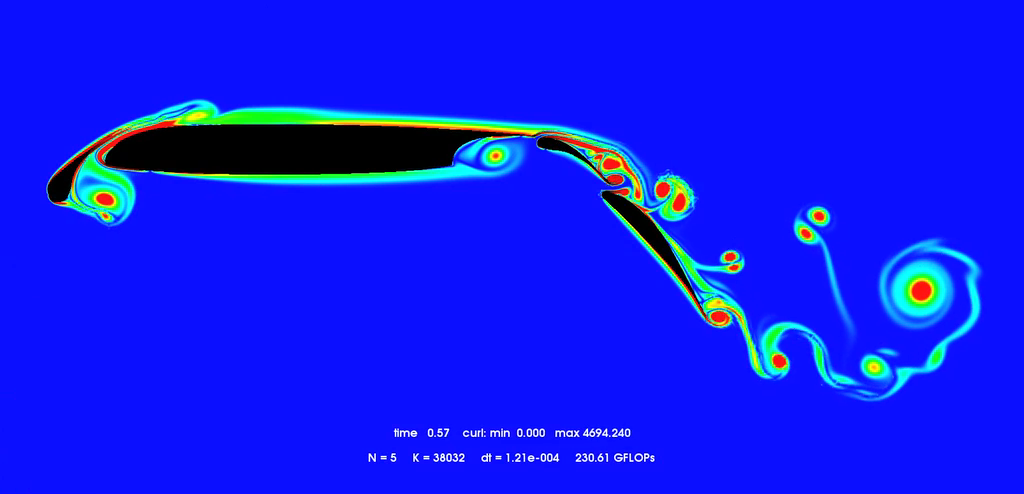
\includegraphics[width=.9\textwidth]{figs/wingflow.png}\\
\vspace{.25em}
\hspace{-.5em}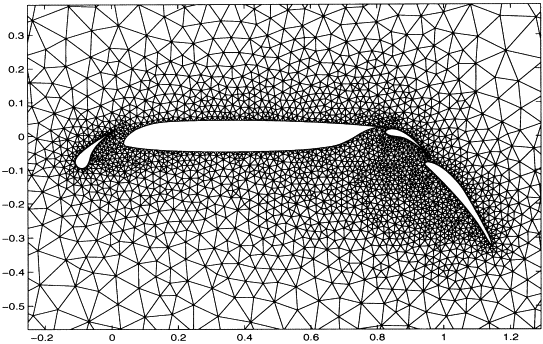
\includegraphics[width=.925\textwidth]{figs/fourfoil.png}
\caption*{\tiny Mesh from Slawig 2001.}
%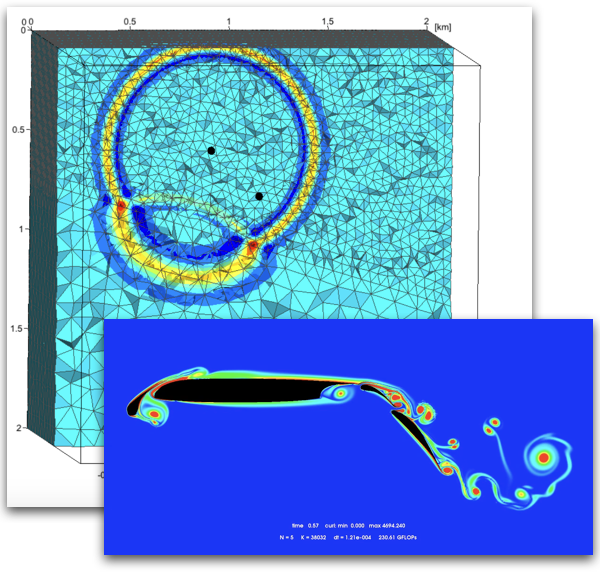
\includegraphics[width=\textwidth]{figs/vortexWave.png}
%%\hspace{-.25em}\hbox{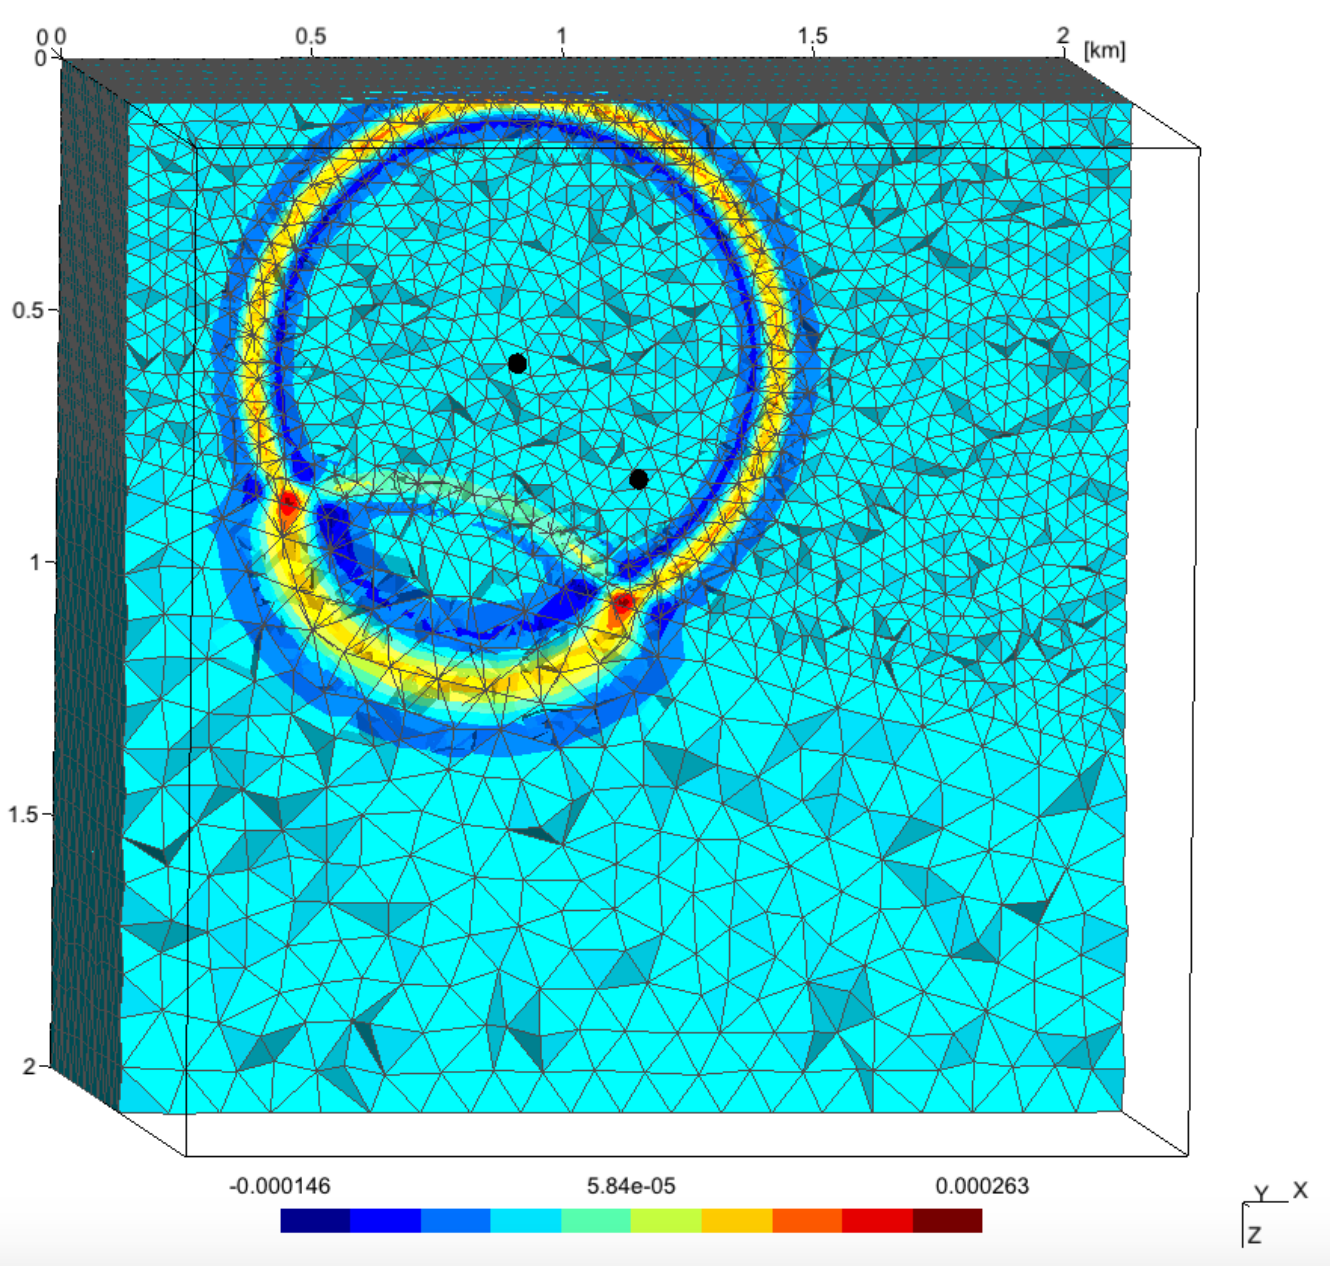
\includegraphics[width=.825\textwidth]{figs/wave.png}}\\
%%\vspace{-5.5em}
%%\hspace{10em}\hbox{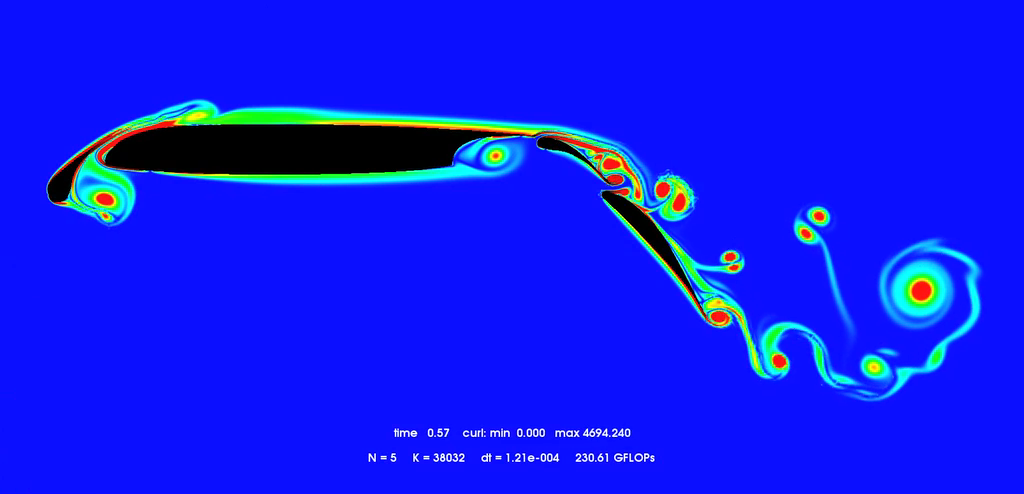
\includegraphics[width=.825\textwidth]{figs/wingflow.png}}
%\caption*{\tiny Figures courtesy of T.\ Warburton, A.\ Modave.}
}
\only<2>{
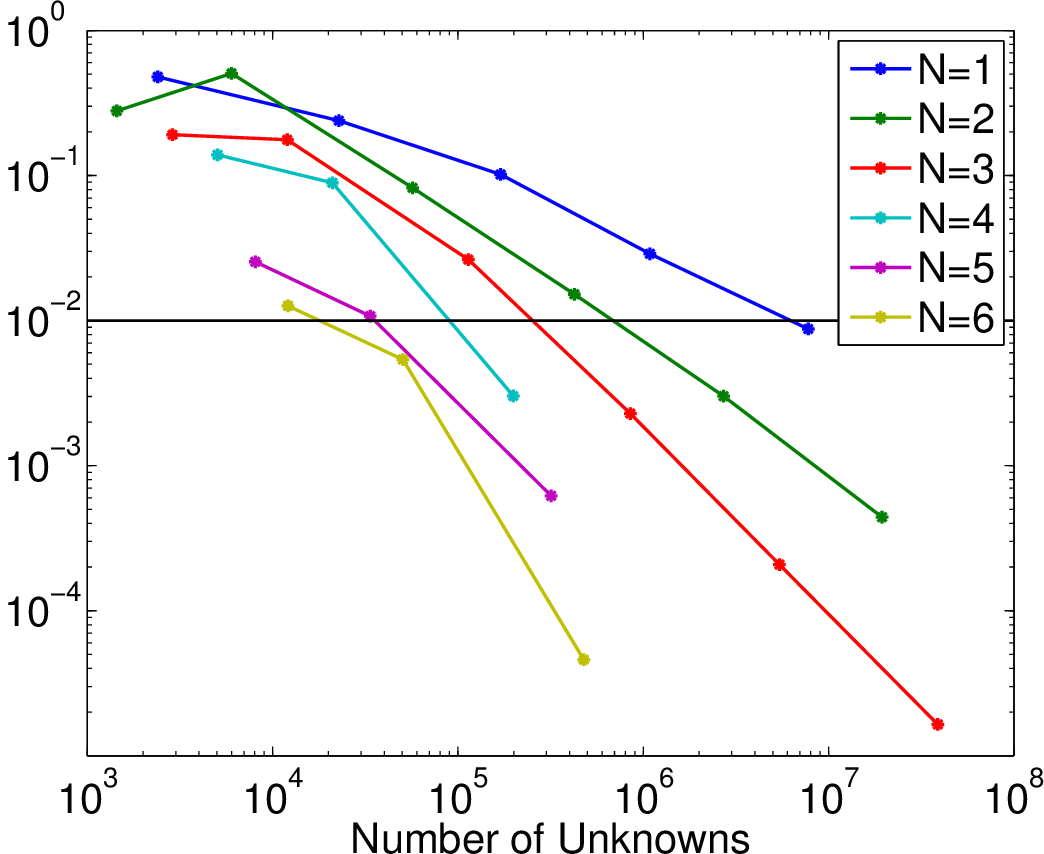
\includegraphics[width=.95\textwidth]{figs/error_v_dofs.png}
\caption*{\scriptsize For smooth solutions, high order methods deliver a lower error per degree of freedom.}
%\includegraphics[width=.95\textwidth]{figs/wave_N1.eps}
%\caption*{\textbf{Fine} linear approximation.}
}
%\only<3>{
%\includegraphics[width=.95\textwidth]{figs/wave_N2.eps}
%\caption*{\textbf{Coarse} quadratic approximation.}
%}
%\only<4>{
%\vspace{1em}
%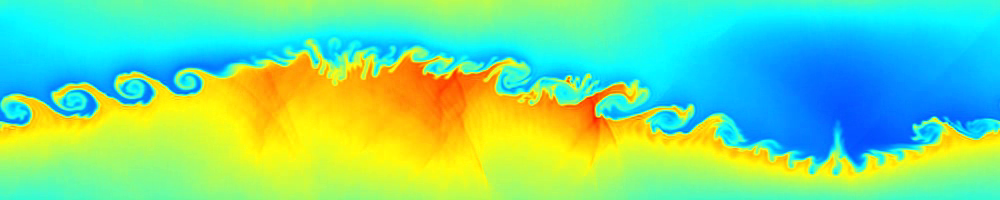
\includegraphics[width=.975\textwidth]{figs/turbulent1.png}\\
%\vspace{.5em}
%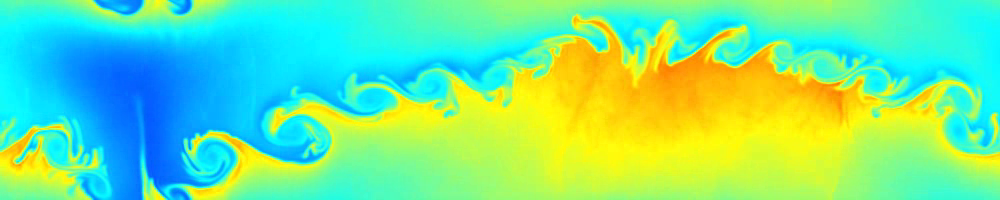
\includegraphics[width=.975\textwidth]{figs/turbulent2.png}
%\caption*{\tiny Figure from Per-Olof Persson.}
%}
\only<3->{
\vspace{1em}
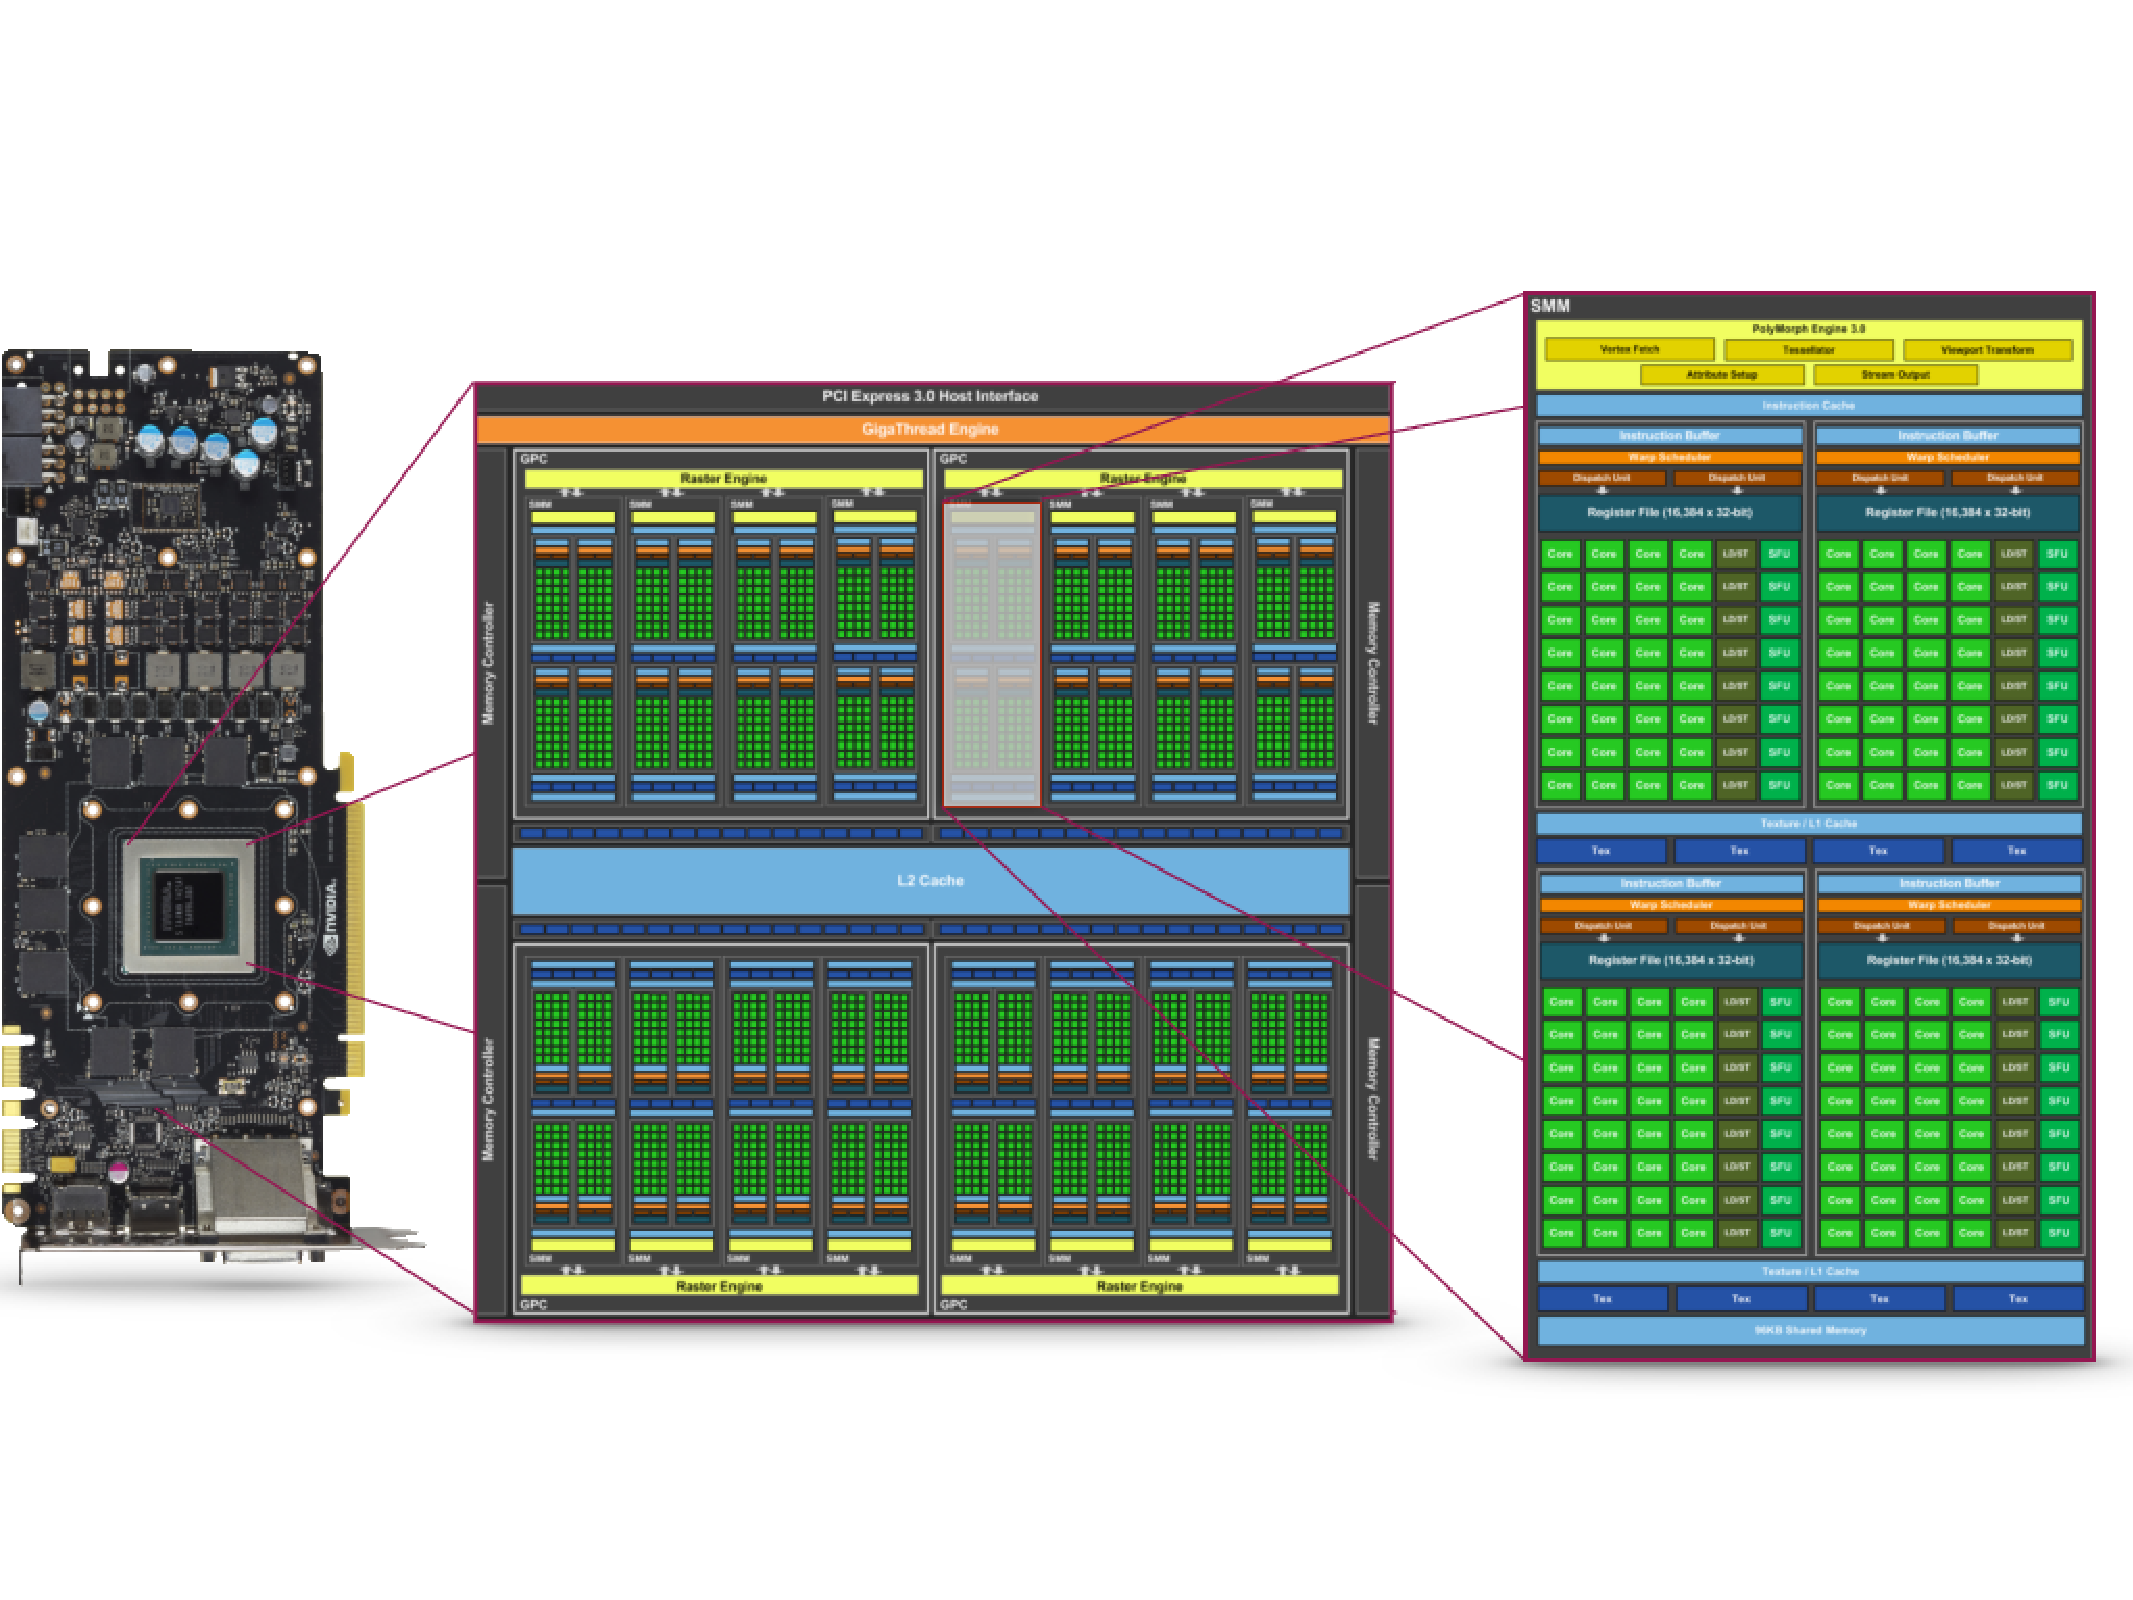
\includegraphics[width=.975\textwidth]{figs/gpu.pdf}
\caption*{\footnotesize Schematic of an NVIDIA graphics processing unit (GPU).}
}
%\caption*{Image courtesy of Axel Modave.}
\end{overlayarea}
\end{figure}
\end{column}
\end{columns}
%\vspace{1.5em}
%\uncover<7>{
%\begin{center}
%\ovalbox{Goal: address the \note{stability} of efficient high order methods.}
%\end{center}
%}
\end{overlayarea}
%\visible<1>{\let\thefootnote\relax\footnotetext[1]{\tiny Figures courtesy of T.\ Warburton, A.\ Modave.}}
%\visible<5>{\let\thefootnote\relax\footnotetext[5]{\tiny Figure courtesy of T.\ Warburton, Nvidia.}}
}

\frame{
\frametitle{Why FEM?  Theory on general unstructured meshes}

\begin{figure}
\centering
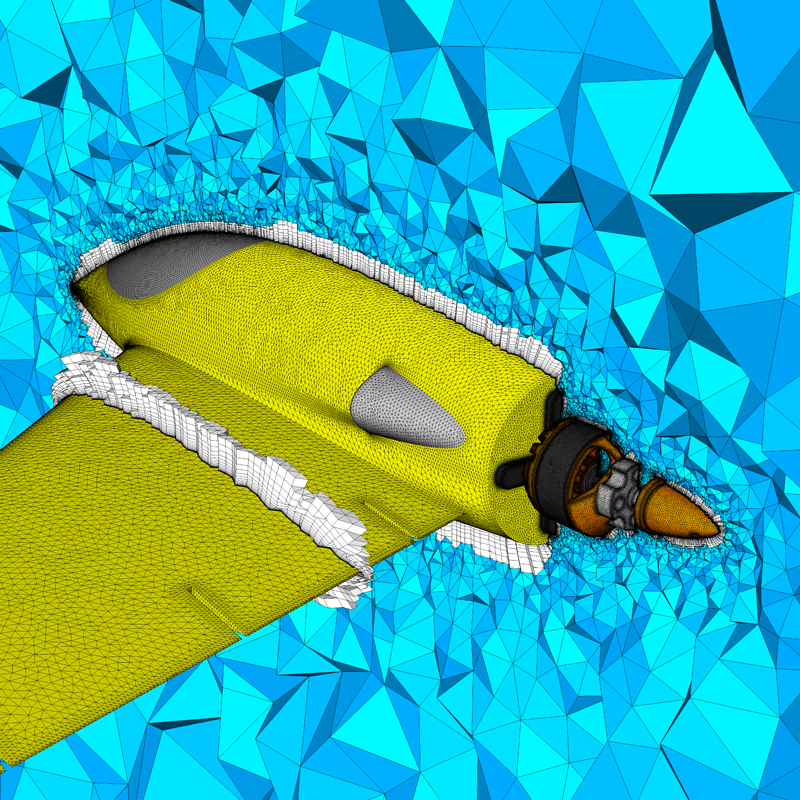
\includegraphics[width=.425\textwidth]{figs/unstructured_mesh1.png}
\hspace{.05em}
\raisebox{2em}{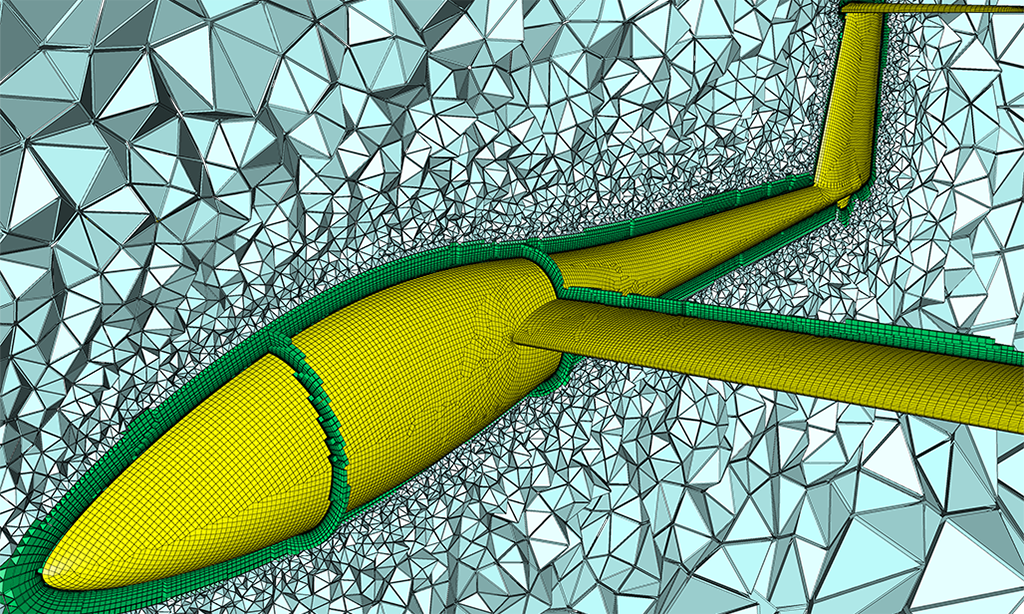
\includegraphics[width=.55\textwidth]{figs/unstructured_mesh2.png}}
\caption*{DG methods are compatible with unstructured meshes containing different types of elements (tetrahedra, hexahedra most common, but also prisms and pyramids).}
\end{figure}

\let\thefootnote\relax\footnotetext[1]{\tiny Figures courtesy of Pointwise Inc (https://www.pointwise.com).}
}


\frame{
\frametitle{Why high order?  Low numerical dissipation}

\begin{figure}
%\only<1>{
%\setcounter{subfigure}{0}
%\centering
%\subfloat[\textbf{Fine} linear approximation]{\includegraphics[width=.475\textwidth]{figs/wave_N1.eps}}
%\hspace{.5em}
%\subfloat[\textbf{Coarse} quadratic approximation]{\includegraphics[width=.475\textwidth]{figs/wave_N2.eps}}
%}
\only<1>{
\setcounter{subfigure}{0}
\centering
\vspace{-.25em}
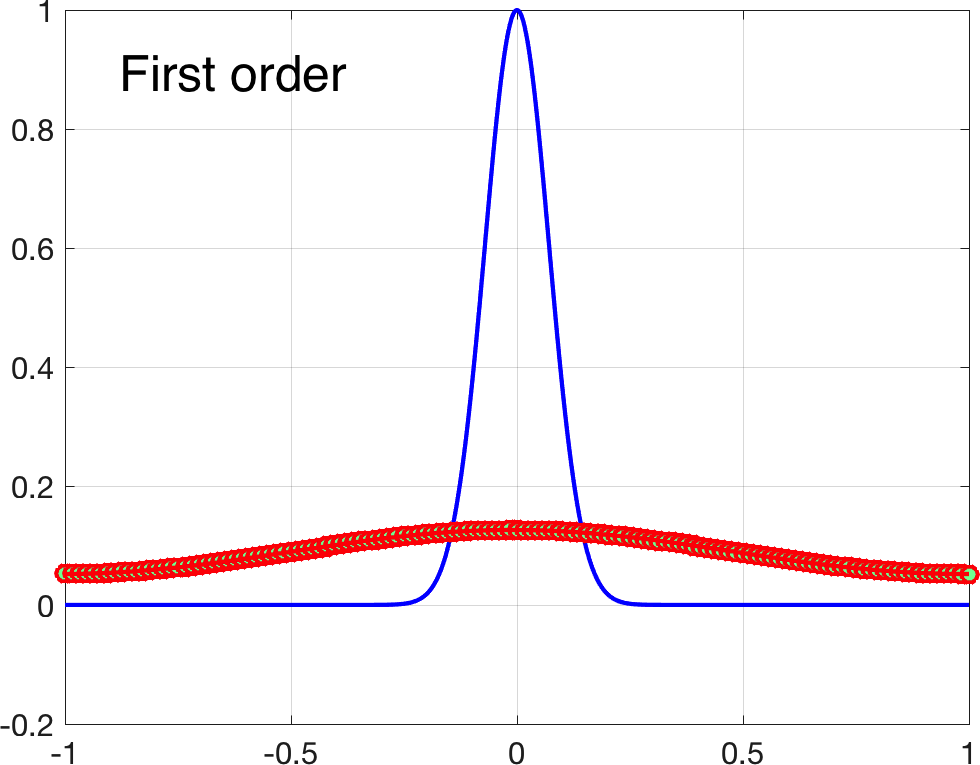
\includegraphics[width=.4\textwidth]{figs/advec1d_N0_diss.png}\hspace{2em}
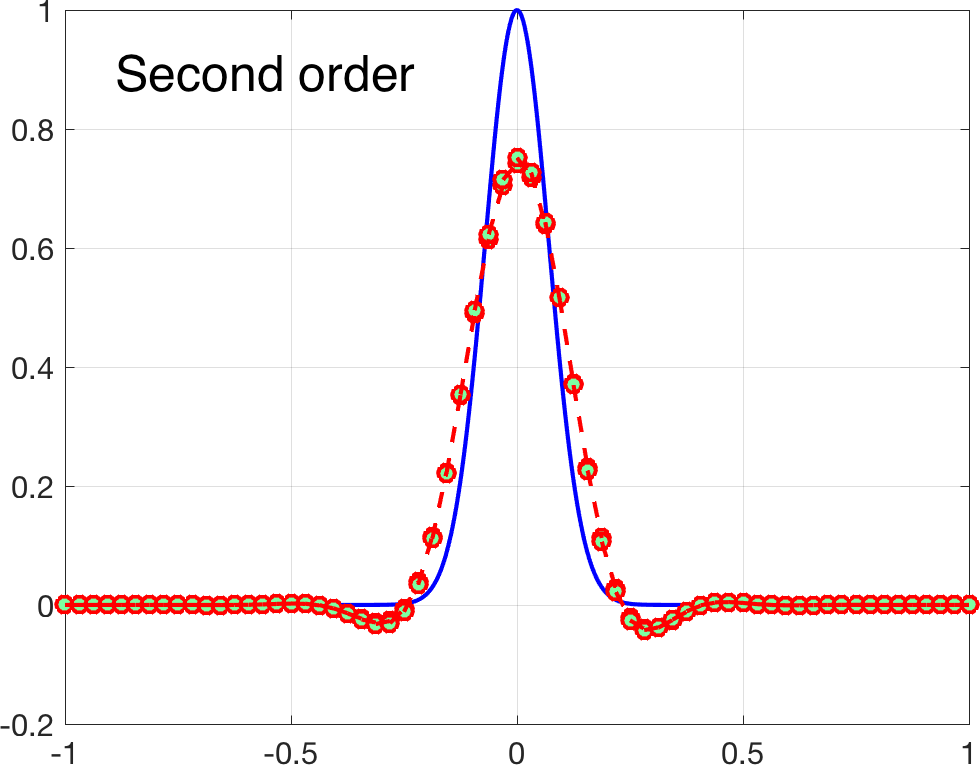
\includegraphics[width=.4\textwidth]{figs/advec1d_N1_diss.png}\\[.5em]
\hspace{.75em}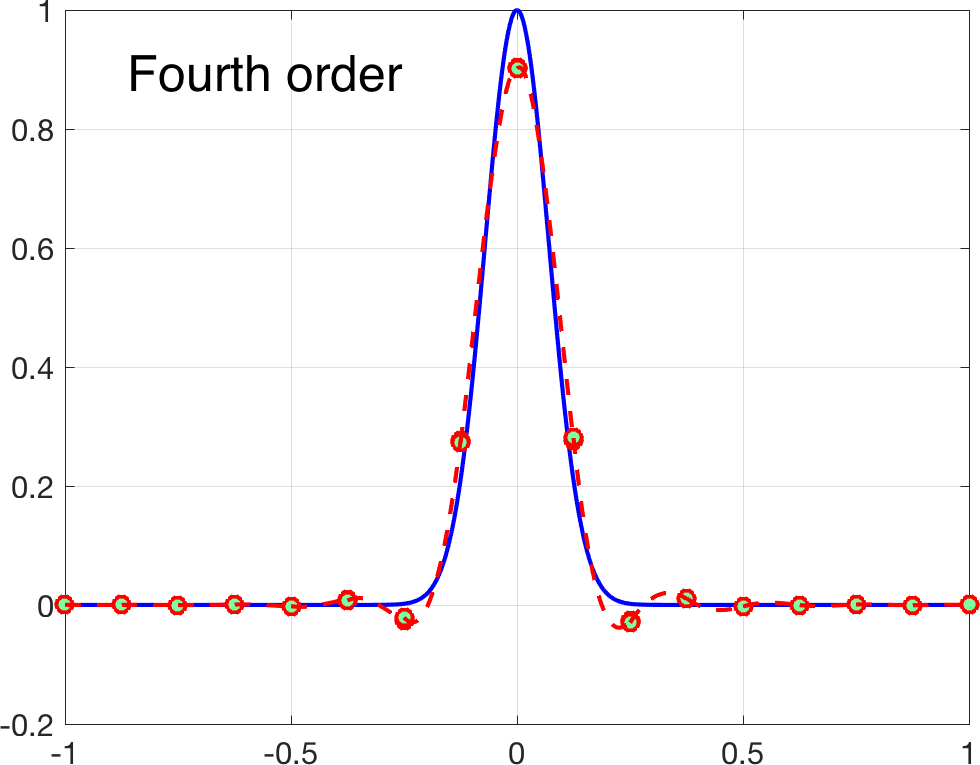
\includegraphics[width=.4\textwidth]{figs/advec1d_N3_diss.png}\hspace{2em}
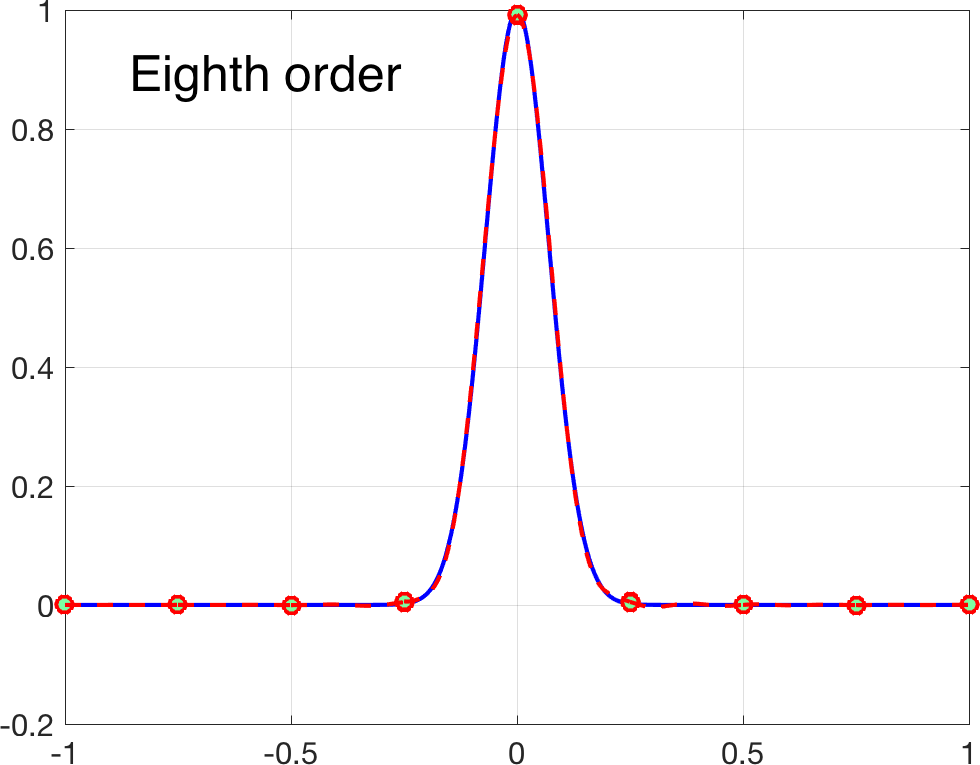
\includegraphics[width=.4\textwidth]{figs/advec1d_N7_diss.png}
}
\only<2>{
\centering
%\vspace{1em}
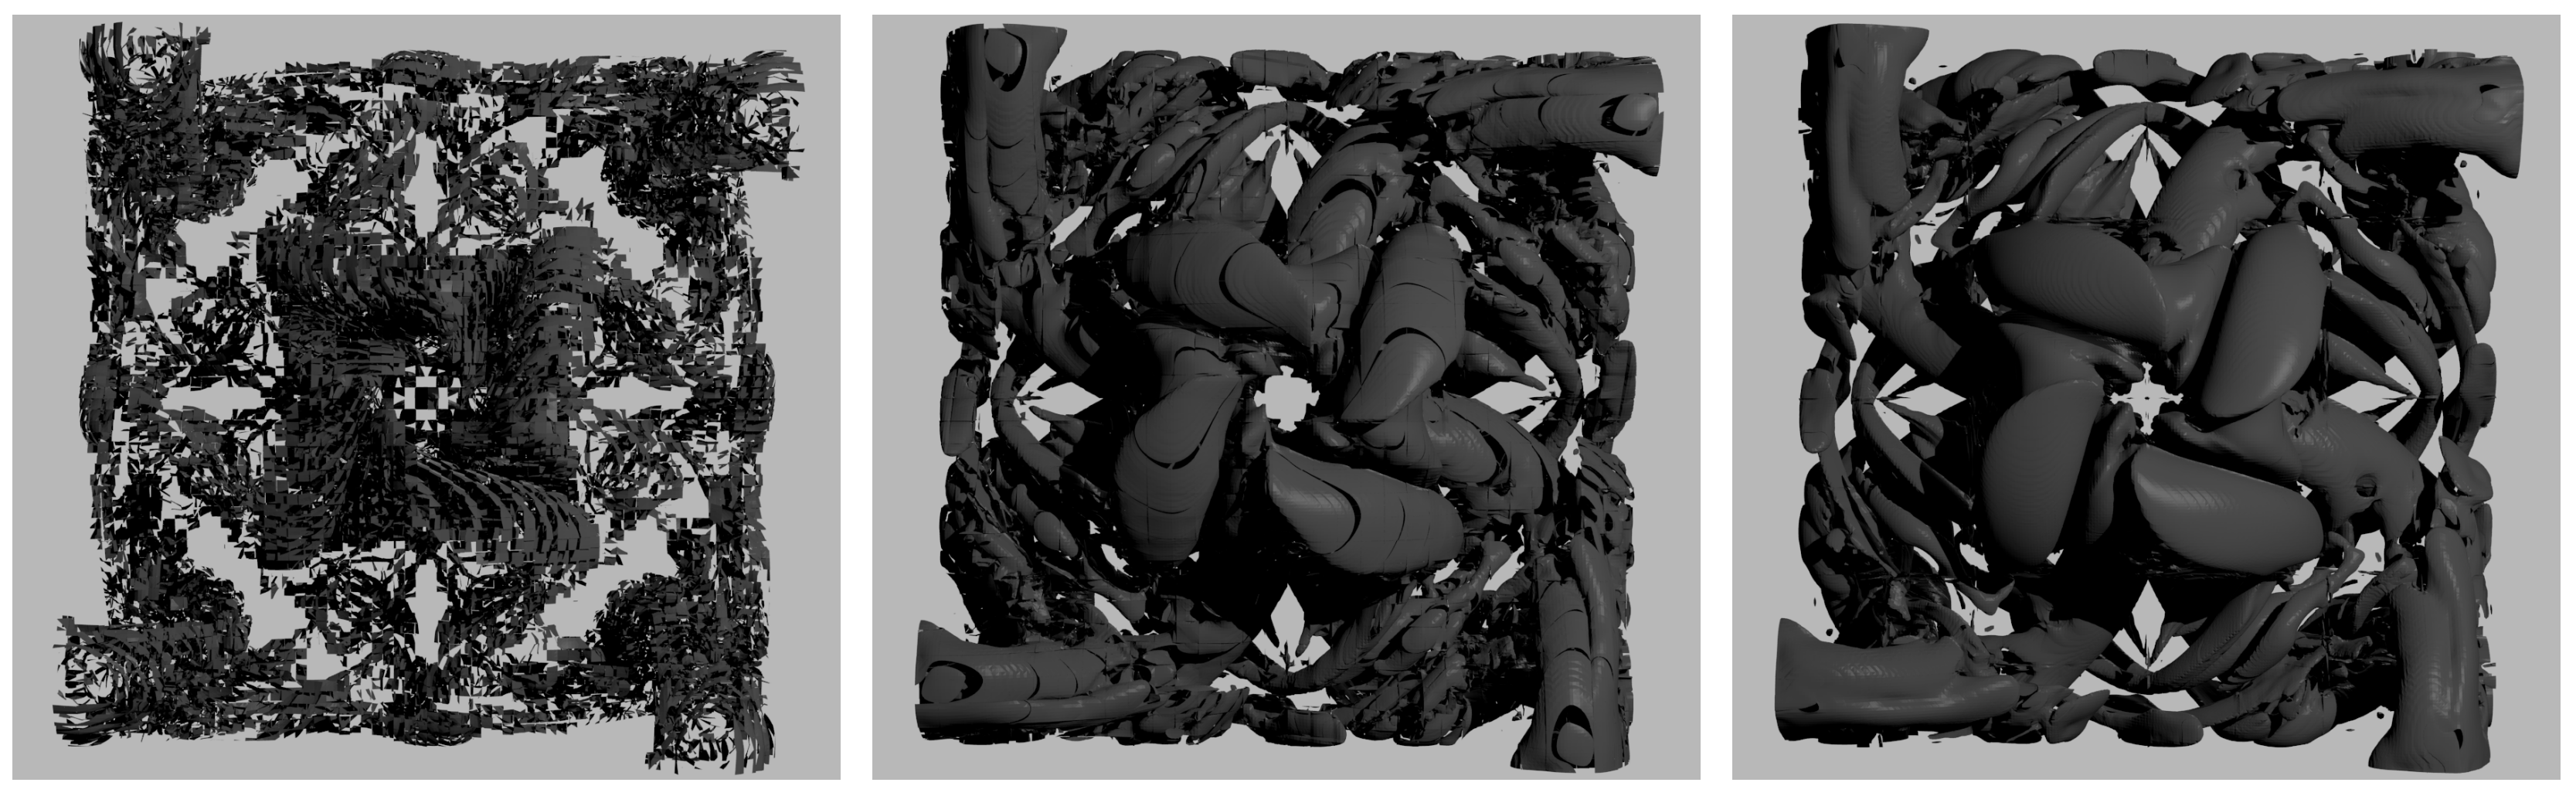
\includegraphics[width=.9\textwidth]{figs/beckgassner.png}\\
\vspace{.25em}
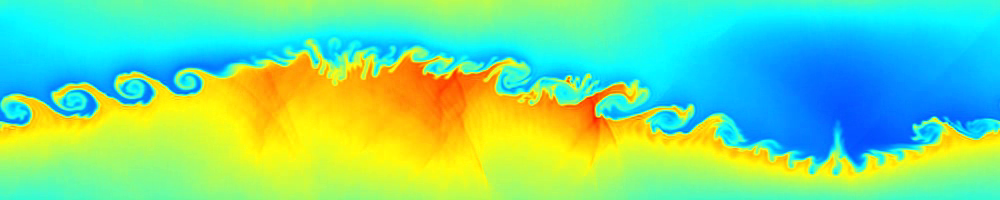
\includegraphics[width=.89\textwidth]{figs/turbulent1.png}%\\
%\vspace{.25em}
%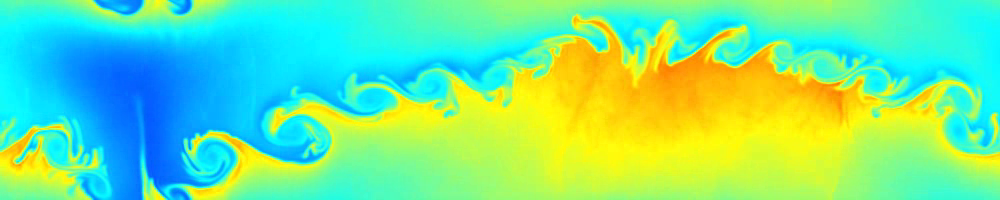
\includegraphics[width=.89\textwidth]{figs/turbulent2.png}
\caption*{\footnotesize 2nd, 4th, and 16th order Taylor-Green (top), 8th order Kelvin-Helmholtz (bottom).}  %Vorticular structures and acoustic waves are both sensitive to numerical dissipation.
}
\end{figure}

\only<2>{
\let\thefootnote\relax\footnotetext{\tiny Beck, Gassner (2012). \emph{Numerical Simulation of the Taylor-Green Vortex at Re=1600 with the Discontinuous Galerkin Spectral Element Method for well-resolved and underresolved scenarios}}
\let\thefootnote\relax\footnotetext{\tiny Peraire, Persson (2010). \emph{High-Order Discontinuous Galerkin Methods for CFD}}
}
}


%\frame{
%\frametitle{What is considered ``high order''?  Waves vs CFD}
%%\vspace{-.5em}
%\begin{columns}
%\begin{column}{.4\textwidth}
%\begin{figure}
%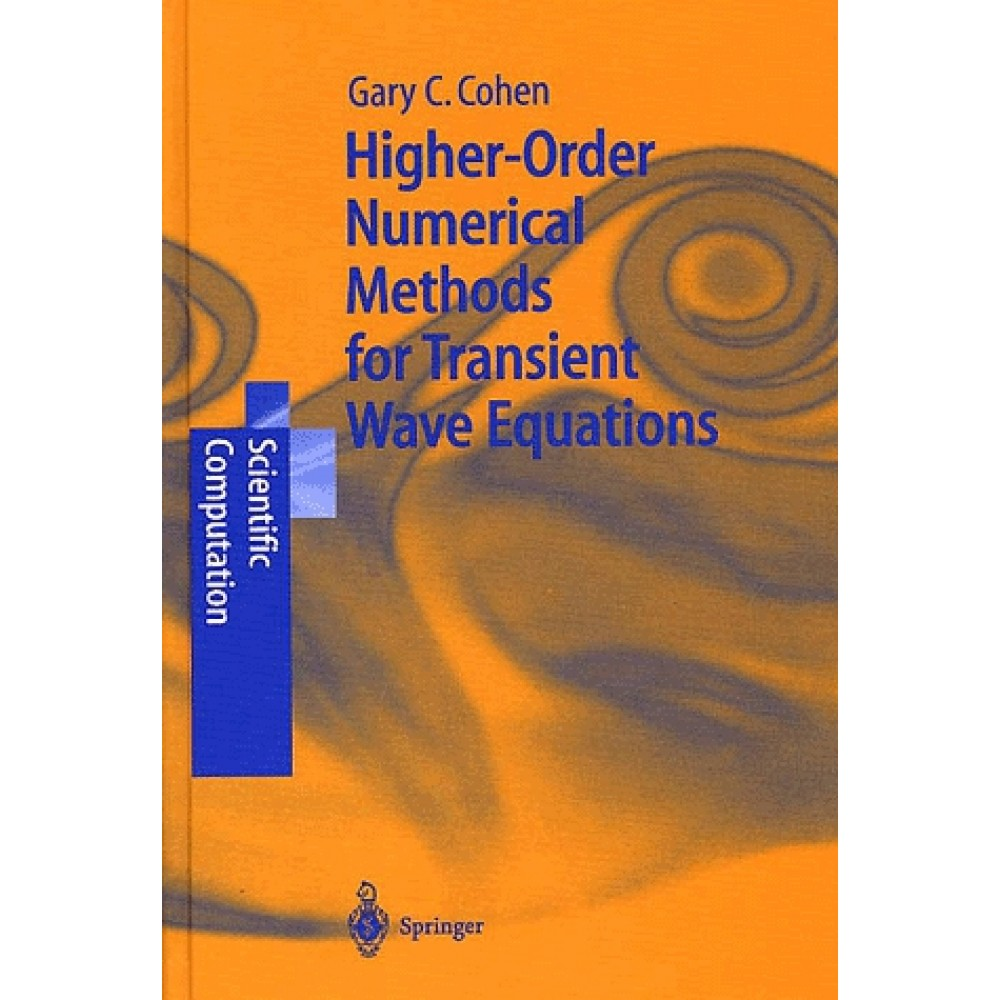
\includegraphics[width=.9\textwidth]{figs/cohenbook.jpg}
%\end{figure}
%\end{column}
%\begin{column}{.6\textwidth}
%\begin{itemize}
%%\item Spectral and $hp$ finite element methods in the 80s
%\item Stability for time-dependent waves, incompressible flow: well established, independent of degree of approx.\ $N$.  
%\vspace{.5em}
%\item High order for waves: $N = 8, 9, 10$ not uncommon (up to $N \approx 20$).  
%\vspace{.5em}
%\item High order for CFD: $N > 1$ (considered much less robust than low order!)
%\end{itemize}
%\end{column}
%\end{columns}
%
%\begin{center}
%\minibox[frame]{Goal: address robustness of efficient high order methods\\
%for time-dependent systems of nonlinear conservation laws.}
%\end{center}
%
%%\let\thefootnote\relax\footnotetext{\tiny Chan, Warburton (2017). \emph{GPU-accelerated Bernstein--Bezier DG methods for wave problems}}
%\let\thefootnote\relax\footnotetext{\tiny Wang, Fidkowski, Abgrall, Bassi, Caraeni, Cary, Deconinck, Hartmann, Hillewaert, Huynh, and Kroll (2013). \emph{High-order CFD methods: current status and perspective}.}
%%\let\thefootnote\relax\footnotetext{\tiny Chan, Demkowicz, and Moser (2014). \emph{A DPG method for steady viscous compressible flow}.}
%}

%% =================================================

%\section{High order time-domain DG methods}

%\frame[noframenumbering]{
%\frametitle{Talk outline}
%\tableofcontents
%}
%
%\frame[noframenumbering]{
%\frametitle{Talk outline}
%\tableofcontents[currentsection]
%}

%% =================================================

%\frame{
%\frametitle{Discretizing the PDE: choosing a numerical method}
%%Choose what you want --- for example, I would like:
%%% FD
%\begin{minipage}{\textwidth}
%\begin{minipage}{.5\textwidth}
%Finite difference methods:
%\begin{itemize}
%\item \textcolor{red}{(Block) structured meshes.}
%\item Stencil size grows with order\\of accuracy.
%\end{itemize}
%\end{minipage}
%\begin{minipage}{.5\textwidth}
%\begin{figure}
%\centering
%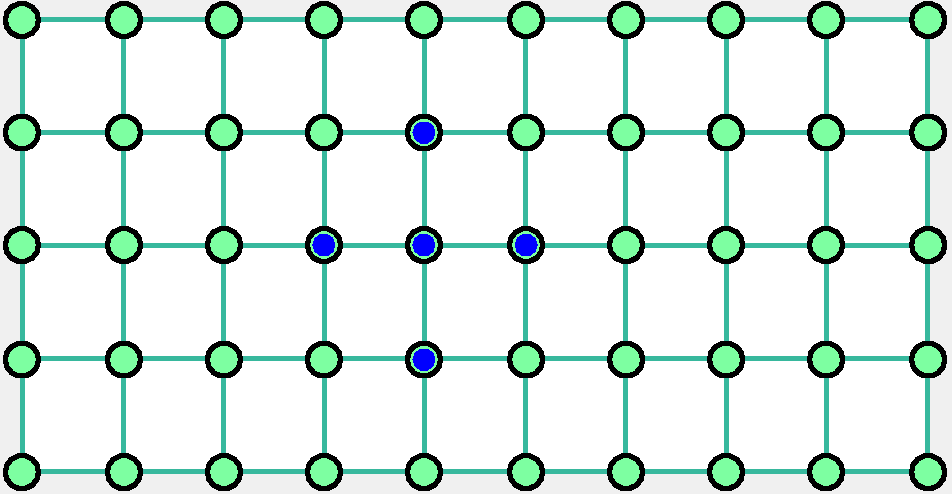
\includegraphics[width=.8\textwidth]{figs/finite_diff.pdf}
%\end{figure}
%\end{minipage}
%\end{minipage}
%
%\vspace{.5em}
%%% FV
%\begin{minipage}{\textwidth}
%\begin{minipage}{.5\textwidth}
%Finite volume methods:
%\begin{itemize}
%\item Complex geometries: unstructured meshes.
%\item \textcolor{red}{Typically low order accurate.}
%\end{itemize}
%
%\end{minipage}
%\begin{minipage}{.5\textwidth}
%\begin{figure}
%\centering
%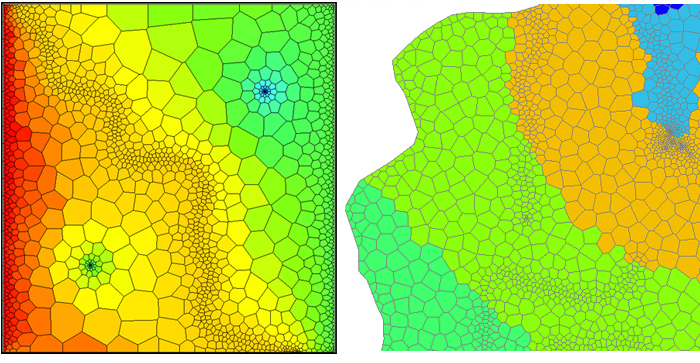
\includegraphics[width=.8\textwidth]{figs/finite_volume.png}
%\end{figure}
%\end{minipage}
%\end{minipage}
%
%\vspace{1em}
%Goals: 
%\begin{itemize}
%\item Flexibility: approximation of solution over complex geometries.
%\item Accuracy: high order methods (mesh size $h$, error $\propto h^{N+1}$). 
%\end{itemize}
%
%\let\thefootnote\relax\footnotetext{\tiny http://www.novametrixgm.com/graphics/blog/finite-volume-method.jpg}
%}
%

%\frame{
%\frametitle{Finite element methods}
%
%\vspace{-.75em}
%\begin{overlayarea}{\textwidth}{\textheight}
%%\vspace{-1em}
%%% FEM
%\begin{columns}
%\begin{column}{.65\textwidth}
%Finite element methods (FEM):
%\vspace{.5em}
%\begin{itemize}
%\item Unstructured meshes.
%\vspace{.5em}
%\item Continuous piecewise polynomial approximation.
%\end{itemize}
%\end{column}
%
%\begin{column}{.35\textwidth}
%\begin{figure}
%\centering
%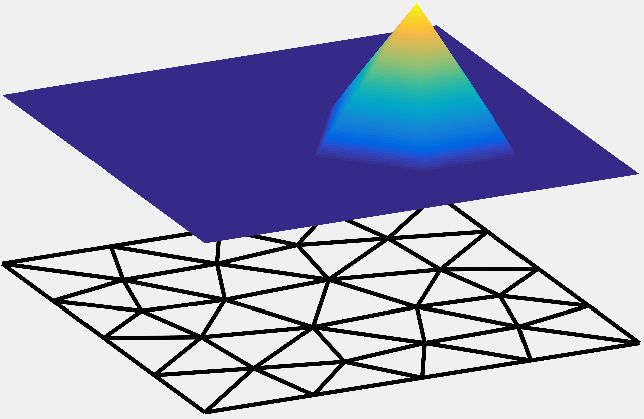
\includegraphics[width=\textwidth]{figs/cg.pdf}
%\end{figure}
%\end{column}
%\end{columns}
%
%\only<1>{
%\vspace{.5em}
%\begin{itemize}
%\item Continuous PDE (example: advection)
%\[
%\pd{u}{t}{} = \pd{u}{x}{}%\div \mathbf{F}(u).
%\]
%\item FEM weak form over domain $\Omega$
%\[
%\int_{\Omega}\pd{u}{t}{} \phi = \int_{\Omega}{\pd{u}{x}{}\phi}, \quad u,\phi \in V_h
%\]
%\end{itemize}
%}
%\only<2>{
%\vspace{-.5em}
%\begin{columns}
%\begin{column}{.65\textwidth}
%FEM yields system of ODEs with\\global mass matrix $\mathbf{M}_{\Omega}$, discretization matrix $\mathbf{A}$.
%\[
%\mathbf{M}_{\Omega}\td{\mathbf{u}}{t} = \mathbf{A}\mathbf{u}.%, \qquad \LRp{\mathbf{M}_{\Omega}}_{ij} = \int_{\Omega} \phi_j\phi_i.
%\]
%FEM mass matrix is \textcolor{red}{globally coupled.}
%\end{column}
%\begin{column}{.35\textwidth}
%\begin{figure}
%\centering
%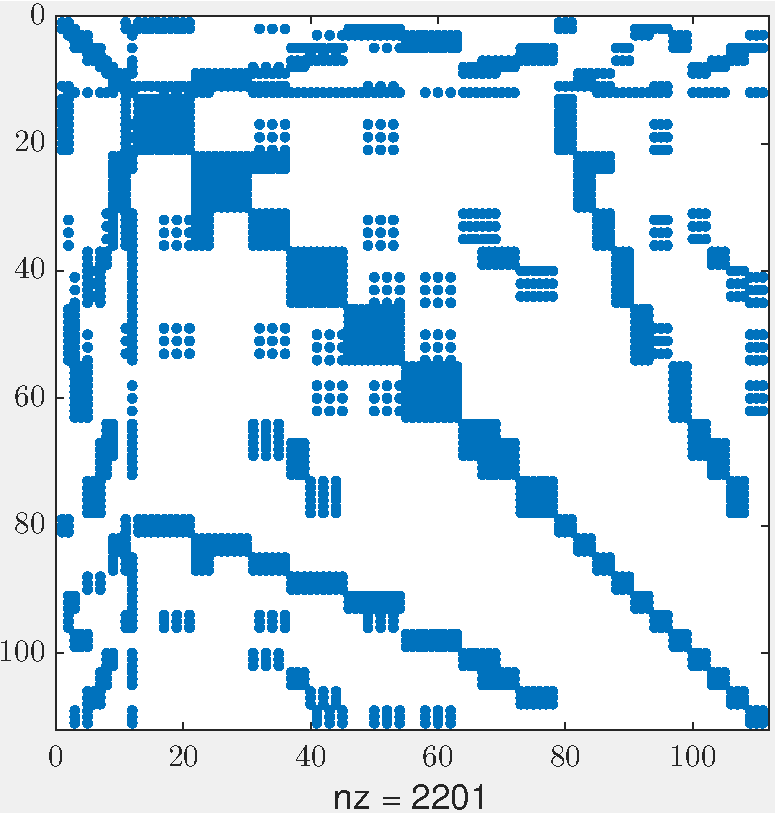
\includegraphics[width=\textwidth]{figs/MCG.pdf}
%%\caption*{\scriptsize Globally coupled FEM mass matrix.}
%\end{figure}
%\end{column}
%\end{columns}
%}
%\end{overlayarea}
%}

\section{Stability of high order DG: linear vs nonlinear PDEs} 


\frame[noframenumbering]{
\frametitle{Talk outline}
\tableofcontents
}

\frame[noframenumbering]{
\frametitle{Talk outline}
\tableofcontents[currentsection]
}



\frame{
\frametitle{Basics of discontinuous Galerkin methods}

\vspace{-.75em}
\begin{overlayarea}{\textwidth}{\textheight}
\begin{columns}
\begin{column}{.65\textwidth}
Discontinuous Galerkin (DG) methods: 
\vspace{.5em}
\begin{itemize}
\item High order accuracy, geometric flexibility.
\vspace{.5em}
\item Weak continuity across faces.
\end{itemize}
\end{column}

\begin{column}{.35\textwidth}
\vspace{-.5em}
\begin{figure}
\centering
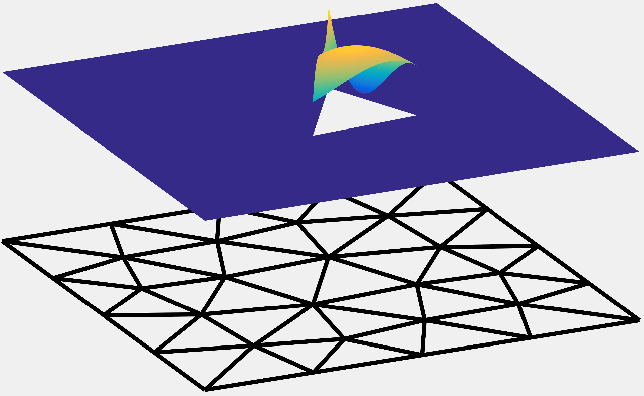
\includegraphics[width=\textwidth]{figs/dg.pdf}
\end{figure}
\end{column}
\end{columns}

\only<1>{
\vspace{.5em}
\begin{itemize}
\item Continuous PDE (example: advection)
\[
\pd{u}{t}{} + \pd{u}{x}{} = 0.%, \qquad f(u) = u.
\]
\item Local DG form with numerical flux $u^*$: find $u \in P^N\LRp{D^k}$ such that
\[
\int_{D_k}\LRp{\pd{u}{t}{} + \pd{u}{x}{}}\phi + \int_{\partial D_k}{{n}_x \LRp{u^*-u}\phi} = 0, \qquad \forall \phi \in P^N\LRp{D^k}.
\]
\end{itemize}
}
\only<2-3>{
\begin{columns}
\begin{column}{.65\textwidth}
Discretizing in space yields system of ODEs %with\\global mass matrix $\mathbf{M}_{\Omega}$, discretization matrix $\mathbf{A}$.
\[
\bm{M}_{\Omega}\td{\bm{u}}{t} = \bm{A}\bm{u}. %\qquad \LRp{\mathbf{M}_{\Omega}}_{ij} = \int_{\Omega} \phi_j\phi_i.
\]
DG mass matrix decouples across elements,\\inter-element coupling only through $\bm{A}$.

\uncover<3>{
\begin{center}
\ovalbox{Goal: ensure ODE system is \note{stable} in time.}
\end{center}
}
\end{column}
\begin{column}{.35\textwidth}
%\vspace{.5em}
\begin{figure}
\centering
\raisebox{.75em}{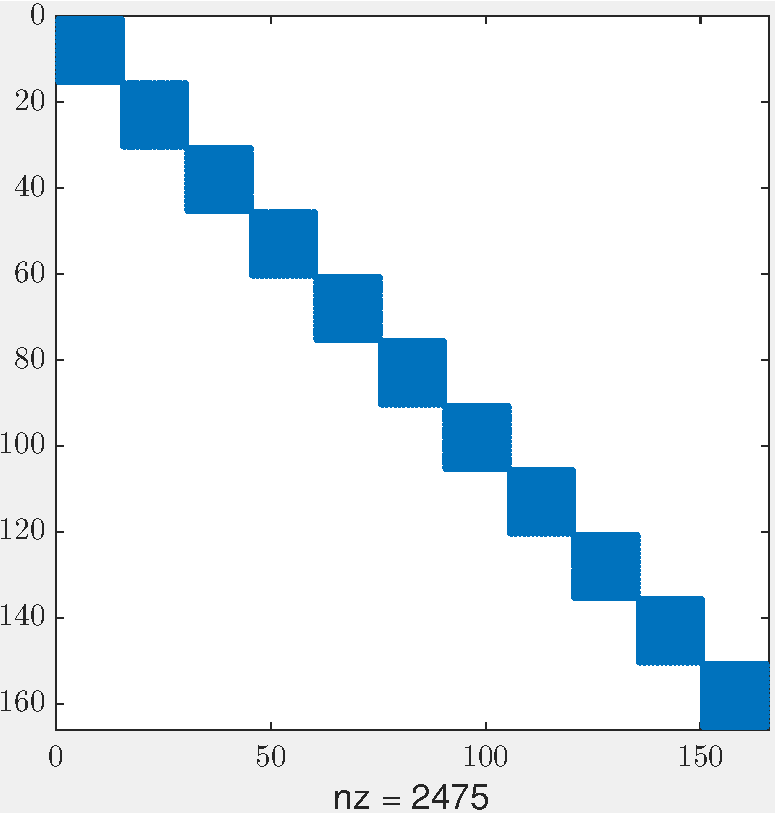
\includegraphics[width=\textwidth]{figs/MDG.pdf}}
%\vspace{-.33em}
%\caption*{\tiny Global mass matrix $\bm{M}_{\Omega}$.}
\end{figure}
\end{column}
\end{columns}
}
\end{overlayarea}
}

%\frame{
%\frametitle{High order nodal discontinuous Galerkin methods}
%\vspace{-.5em}
%\begin{figure}
%\centering
%\subfloat{\includegraphics[width=.24\textwidth]{figs/nodal1D.eps}}
%\subfloat{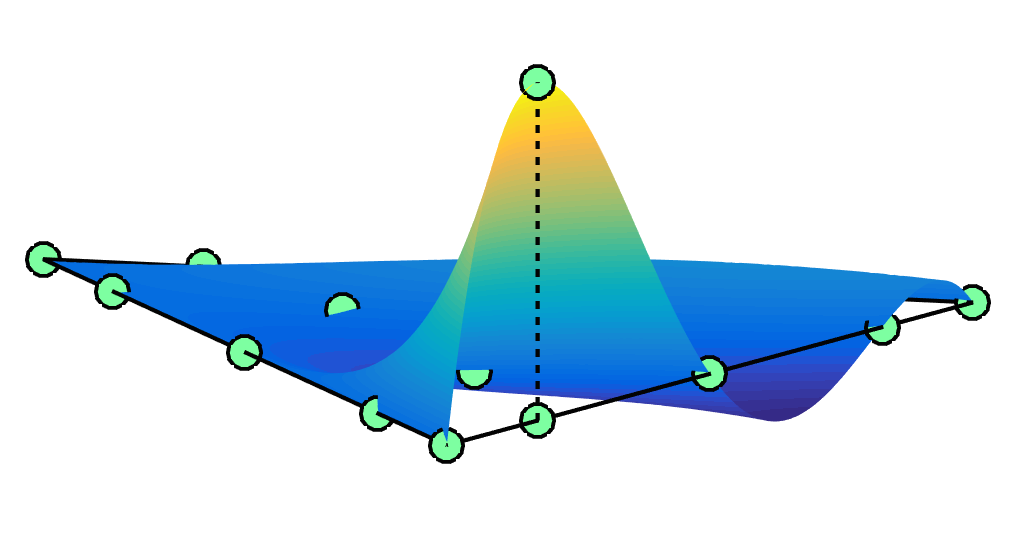
\includegraphics[width=.4\textwidth]{figs/nodal2D.png}}
%\hspace{.1em}
%\subfloat{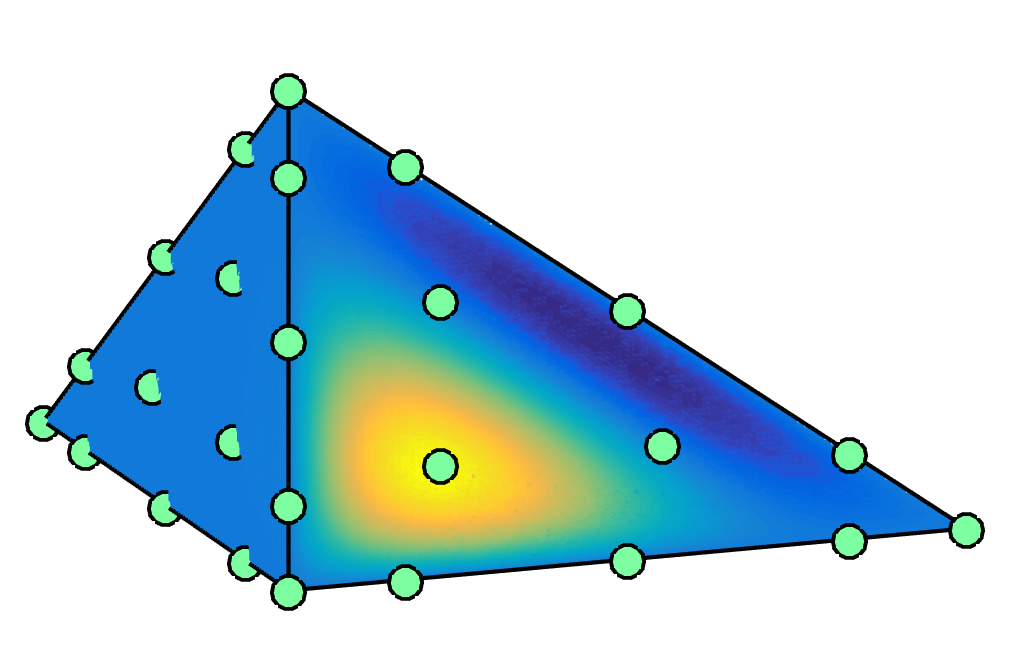
\includegraphics[width=.31\textwidth]{figs/nodal3D.png}}
%\caption*{Lagrange (nodal) bases on a line, triangle, tetrahedron.   }
%\end{figure}
%%\vspace{.5em}
%\begin{itemize}
%\item Nodal bases defined implicitly through an orthogonal basis.  
%\vspace{.5em}
%\item Point locations optimized for interpolation and numerical stability. 
%\vspace{.5em}
%\item Assume \textbf{affine} tetrahedra, coefficients \textbf{constant} on each element.
%%\item Derivative matrices w.r.t.\ reference coordinates $\bm{\widehat{x}} = (r,s,t)$ 
%%\[
%%\LRp{\mathbf{\widehat{D}}_r}_{ij} = \pd{\ell_j(\bm{\widehat{x}}_i)}{r}{}, \qquad \LRp{\mathbf{\widehat{D}}_s}_{ij} = \pd{\ell_j(\bm{\widehat{x}}_i)}{s}{}, \qquad \LRp{\mathbf{\widehat{D}}_t}_{ij} = \pd{\ell_j(\bm{\widehat{x}}_i)}{t}{}.
%%\]
%\end{itemize}
%}

%\frame{
%\frametitle{Implementation of explicit time-domain DG methods}
%%\vspace{-2em}
%\begin{columns}
%\begin{column}{.55\textwidth}
%Given initial condition $u(\mathbf{x},0)$:
%\vspace{.25em}
%\begin{itemize}
%\item<1-> Compute numerical flux on\\element faces (\textcolor{red}{non-local}).
%\vspace{.25em}
%\item<2-> Compute RHS of (\textcolor{blue}{local}) ODE.%: differentiation and lifting matrices.
%\vspace{.25em}
%\item<3-> Evolve  (\textcolor{blue}{local}) solution using \textcolor{red}{explicit} time integration (RK, AB, etc). 
%\end{itemize}
%\end{column}
%\begin{column}{.45\textwidth}
%\begin{figure}
%\centering
%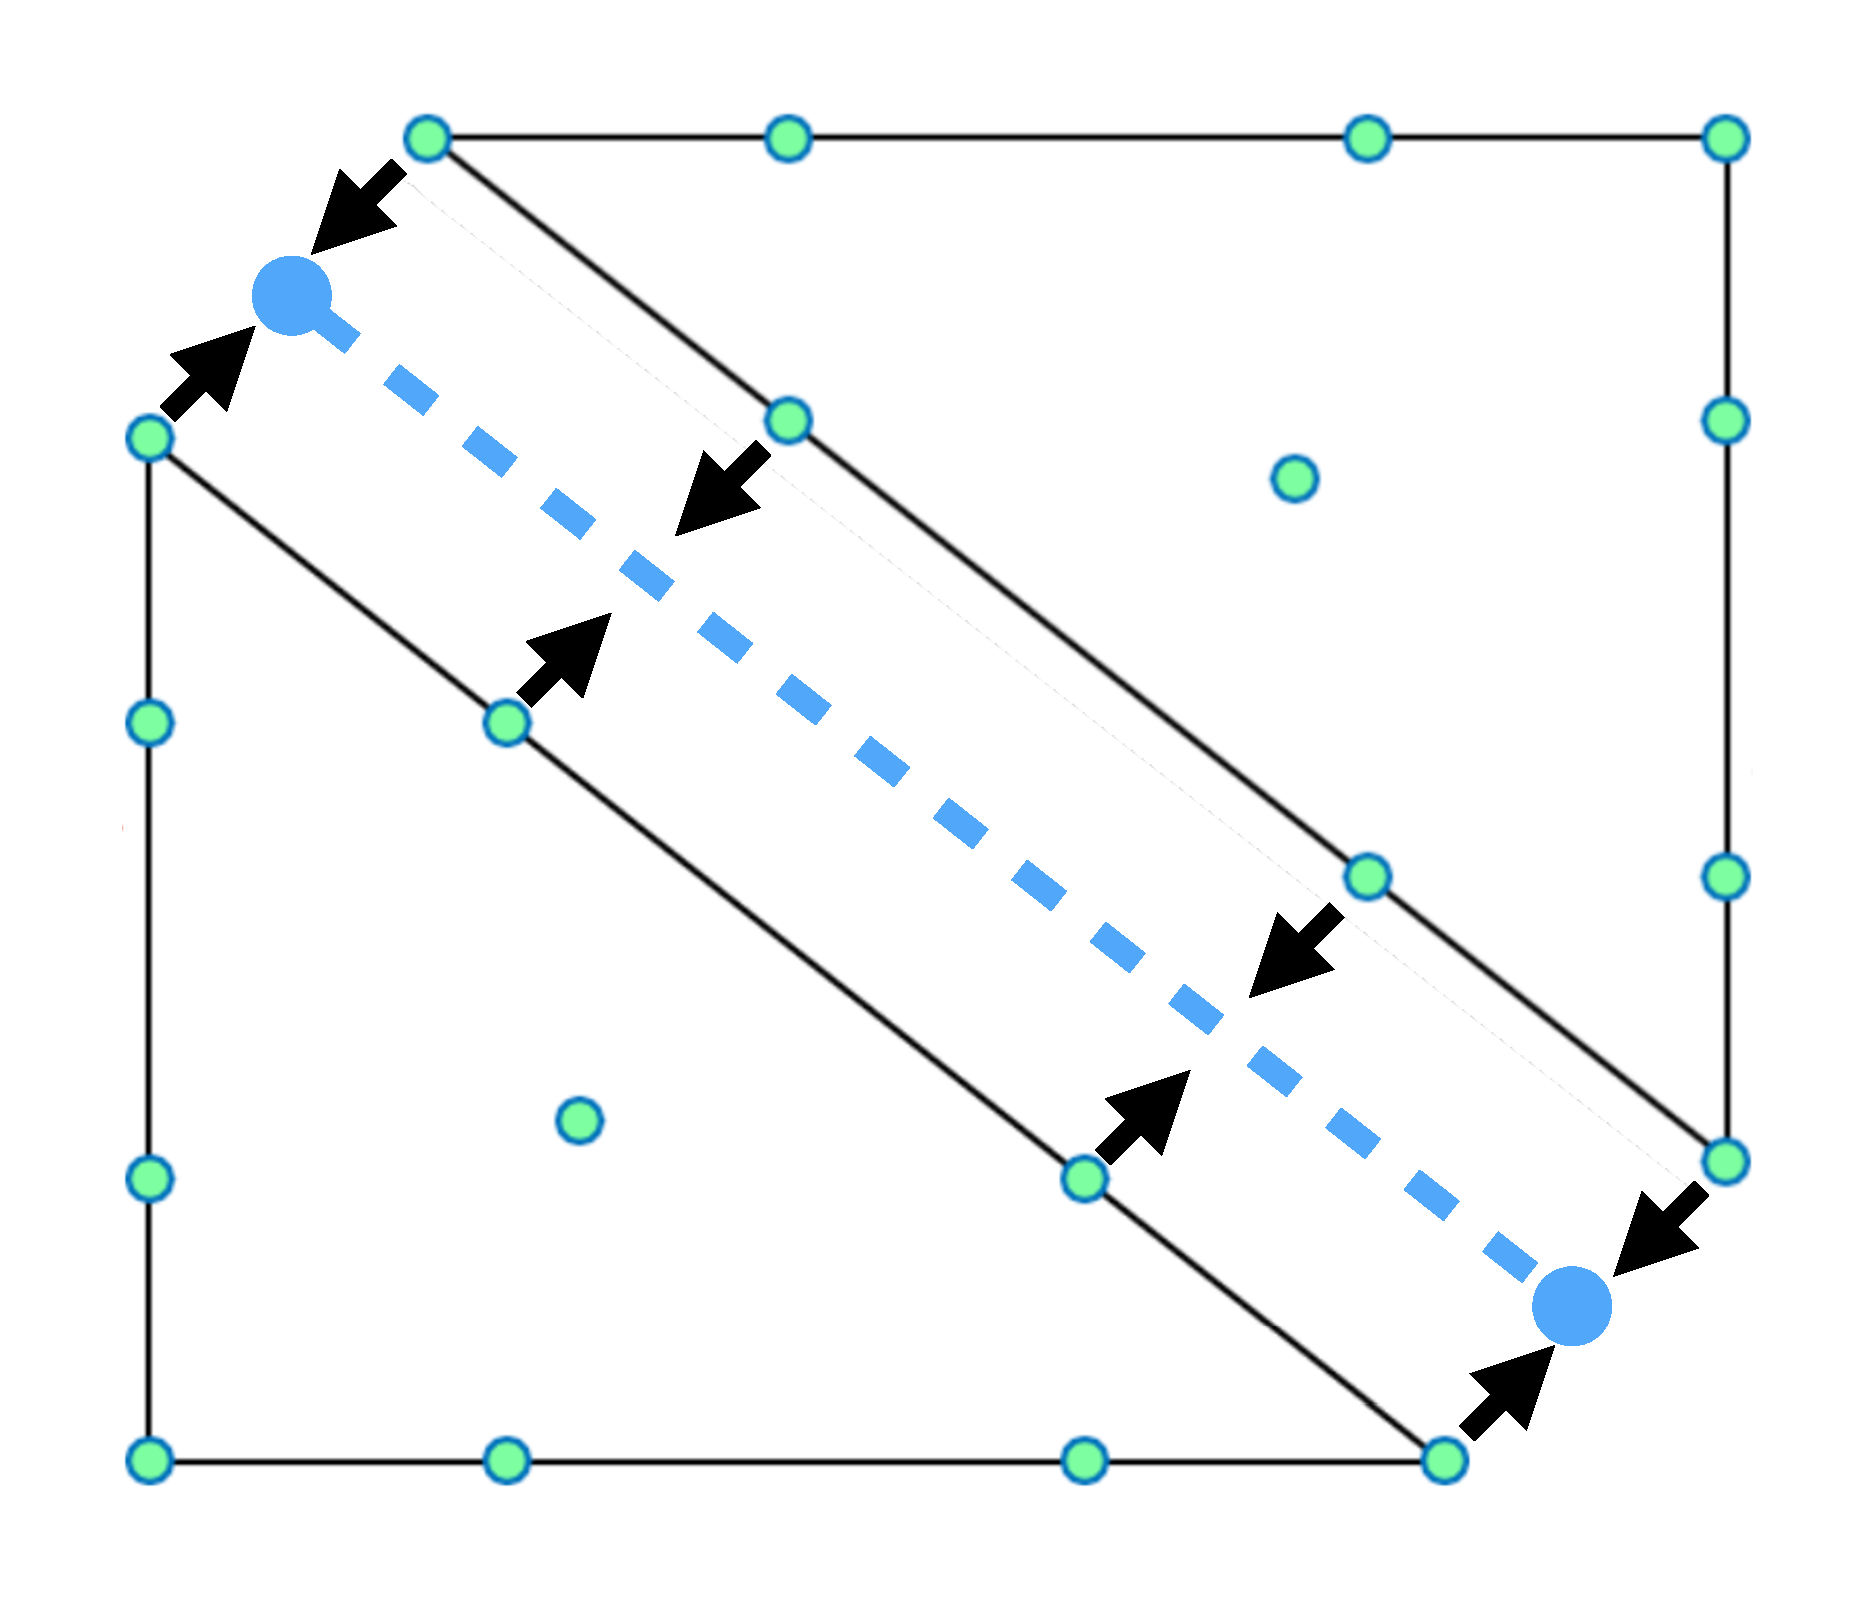
\includegraphics[width=.85\textwidth]{figs/nodal.pdf}
%\end{figure}
%\end{column}
%\end{columns}
%%\vspace{1em}
%\begin{overlayarea}{\textwidth}{.4\textheight}
%\only<1>{\[
%\td{\mathbf{u}}{t} = \mathbf{D}_x \mathbf{u} + \sum_{\text{ faces}}\mathbf{L}_f \LRp{\rm \textcolor{red}{flux}}, \qquad \mathbf{L}_f = \mathbf{{M}}^{-1}\mathbf{{M}}_f.
%\]
%}
%\only<2>{
%\[
%\td{\mathbf{u}}{t} = \underbrace{\mathbf{D}_x \mathbf{u}}_{\text{\textcolor{blue}{Volume}}} + \underbrace{\sum_{\text{ faces}}\mathbf{L}_f \LRp{\rm \textcolor{red}{flux}}}_{\text{\textcolor{blue}{Surface}}}, \qquad \mathbf{L}_f = \mathbf{{M}}^{-1}\mathbf{{M}}_f.
%\]
%}
%\only<3>{
%\[
%\underbrace{\td{\mathbf{u}}{t}}_{\text{\textcolor{blue}{Update}}} = \underbrace{\mathbf{D}_x \mathbf{u}}_{\text{\textcolor{blue}{Volume}}} + \underbrace{\sum_{\text{ faces}}\mathbf{L}_f \LRp{\rm \textcolor{red}{flux}}}_{\text{\textcolor{blue}{Surface}}}, \qquad \mathbf{L}_f = \mathbf{{M}}^{-1}\mathbf{{M}}_f.
%\]
%}
%\only<4>{
%\vspace{.5em}
%\begin{center}
%\textbf{Pros:} simple, scalable, and efficient matrix-free implementation. 
%\\
%\vspace{.5em}
%\textbf{Cons:} explicit time-stepping, high order methods prone to \textcolor{red}{instability}.\\
%Regularization (slope limiting, artificial viscosity) to avoid blow up!
%\\
%\vspace{1em}
%\ovalbox{Must ensure semi-discrete system is inherently \emph{energy stable}!}
%\end{center}
%}
%\end{overlayarea}
%}% frame


\frame{
\frametitle{DG is semi-discretely energy stable for linear advection}

\begin{itemize}
\item<1-> Linear periodic advection on $[-1,1]$
\[
\pd{u}{t} + \pd{u}{x} = 0, \qquad u(-1) = u(1), \qquad \Longrightarrow \pd{}{t}\nor{u}_{L^2([-1,1])}^2 = 0.  
\]
%\item<2-> Triangulate domain with elements $D^k$, 
%\vspace{.5em}
\item<2-> DG numerical ``penalty'' flux, where $\jump{u} = u^+ - u$ and $\tau \geq 0$.
\begin{align*}
%\sum_k 
\sum_{k} \int_{D^k} \LRp{\pd{u}{t} + \pd{u}{x}}v \diff{x} + 
\frac{1}{2}\int_{\partial D^k}\LRp{\jump{u}n_x + \tau\jump{u}}v \diff{x}=0.
%\sum_k\int_{D^k} \LRp{\pd{u}{t} + \pd{u}{x}}v + 
%\int_{\partial D^k} \frac{n_x-\tau\LRb{n_x}}{2} \jump{u}v  = 0, \qquad \forall v \in V_h.
\end{align*}
\item<3-> Energy estimate: take $v = u$, chain rule in time, \textcolor{red}{integrate by parts}.  
\begin{align*}
\sum_k \pd{}{t} \nor{u}_{D^k}^2  \leq -\sum_k \frac{\tau}{2}\int_{\partial D^k}\jump{u}^2 \diff{x}.
%\sum_k\int_{D^k} \LRp{\pd{u}{t} + \pd{u}{x}}v + 
%\int_{\partial D^k} \frac{n_x-\tau\LRb{n_x}}{2} \jump{u}v  = 0, \qquad \forall v \in V_h.
\end{align*}

\end{itemize}
%\vspace{-.5em}
}

\frame{
\frametitle{Energy conservative vs.\ energy stable DG methods}
%\begin{overlayarea}{\textwidth}{.475\textheight}
\begin{itemize}
\item Energy estimate implies that $\nor{u}$ is non-increasing for $\tau \geq 0$.
\vspace{.25em}
\item Energy conservative (non-dissipative) ``central'' flux when $\tau = 0$.
\vspace{.25em}
\item Energy stable (dissipative) ``Lax-Friedrichs'' flux when $\tau = 1$.
\end{itemize} 
\begin{figure}
\centering
\captionsetup[subfloat]{width=.5\textwidth, justification=centering}
\subfloat[Energy conservative ($\tau = 0$)]{
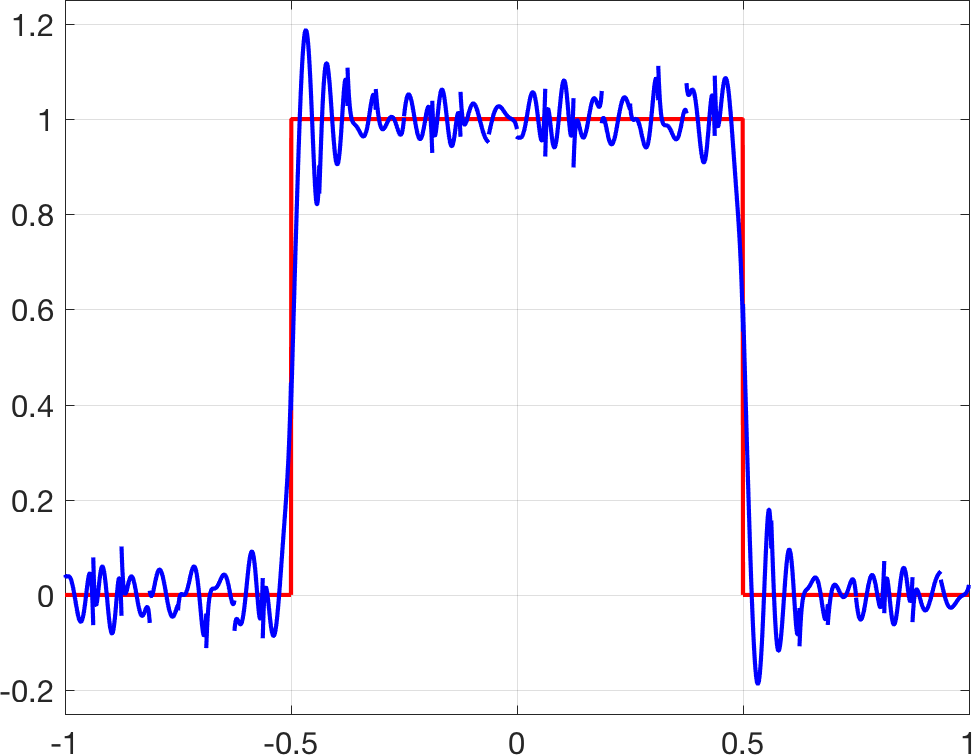
\includegraphics[width=.425\textwidth]{figs/advecCentral.png}}
\hspace{.5em}
\subfloat[Energy stable ($\tau = 1$)]{
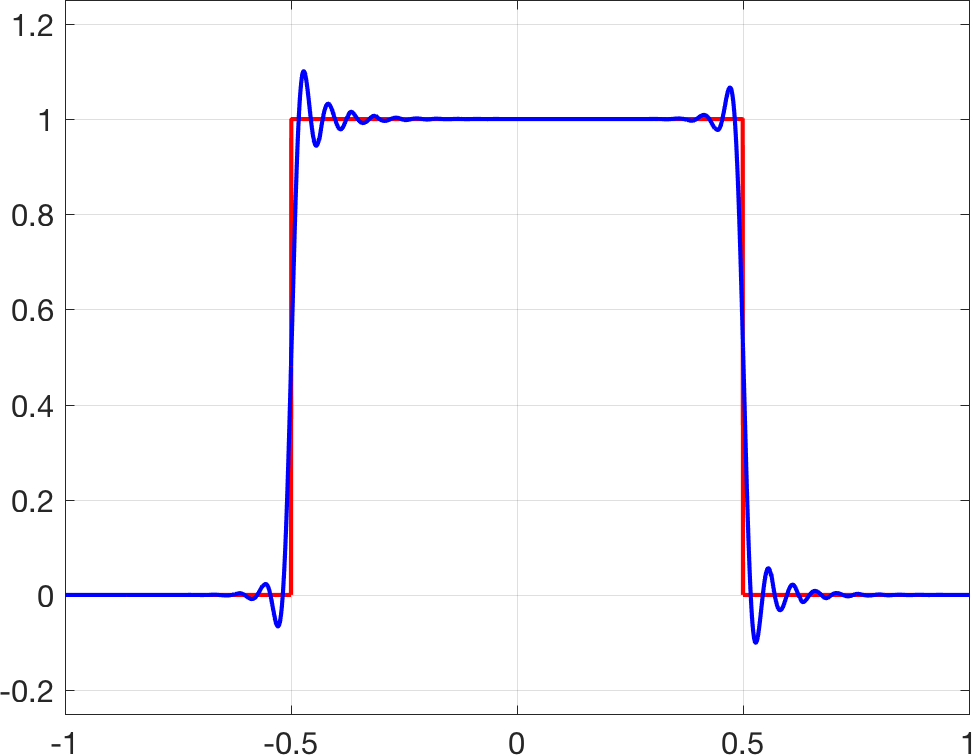
\includegraphics[width=.425\textwidth]{figs/advecUpwind.png}}
\end{figure}
%\end{overlayarea}
}

%% =================================================

%\frame{
%\frametitle{Global DG differentiation operators}
%
%\begin{overlayarea}{\textwidth}{.95\textheight}
%\begin{itemize}
%\item<1-> Let $V_h = \bigoplus_k P^N(D^k)$.  Define jump, average across shared face
%\[
%\jump{u} = u^+ - u, \qquad \avg{u} = \frac{u^+ + u}{2}, \qquad u^+ = u \text{ on boundary}.
%\]
%\only<1>{
%\vspace{-.5em}
%\begin{figure}
%%\centering
%\hspace{-3em}\hbox{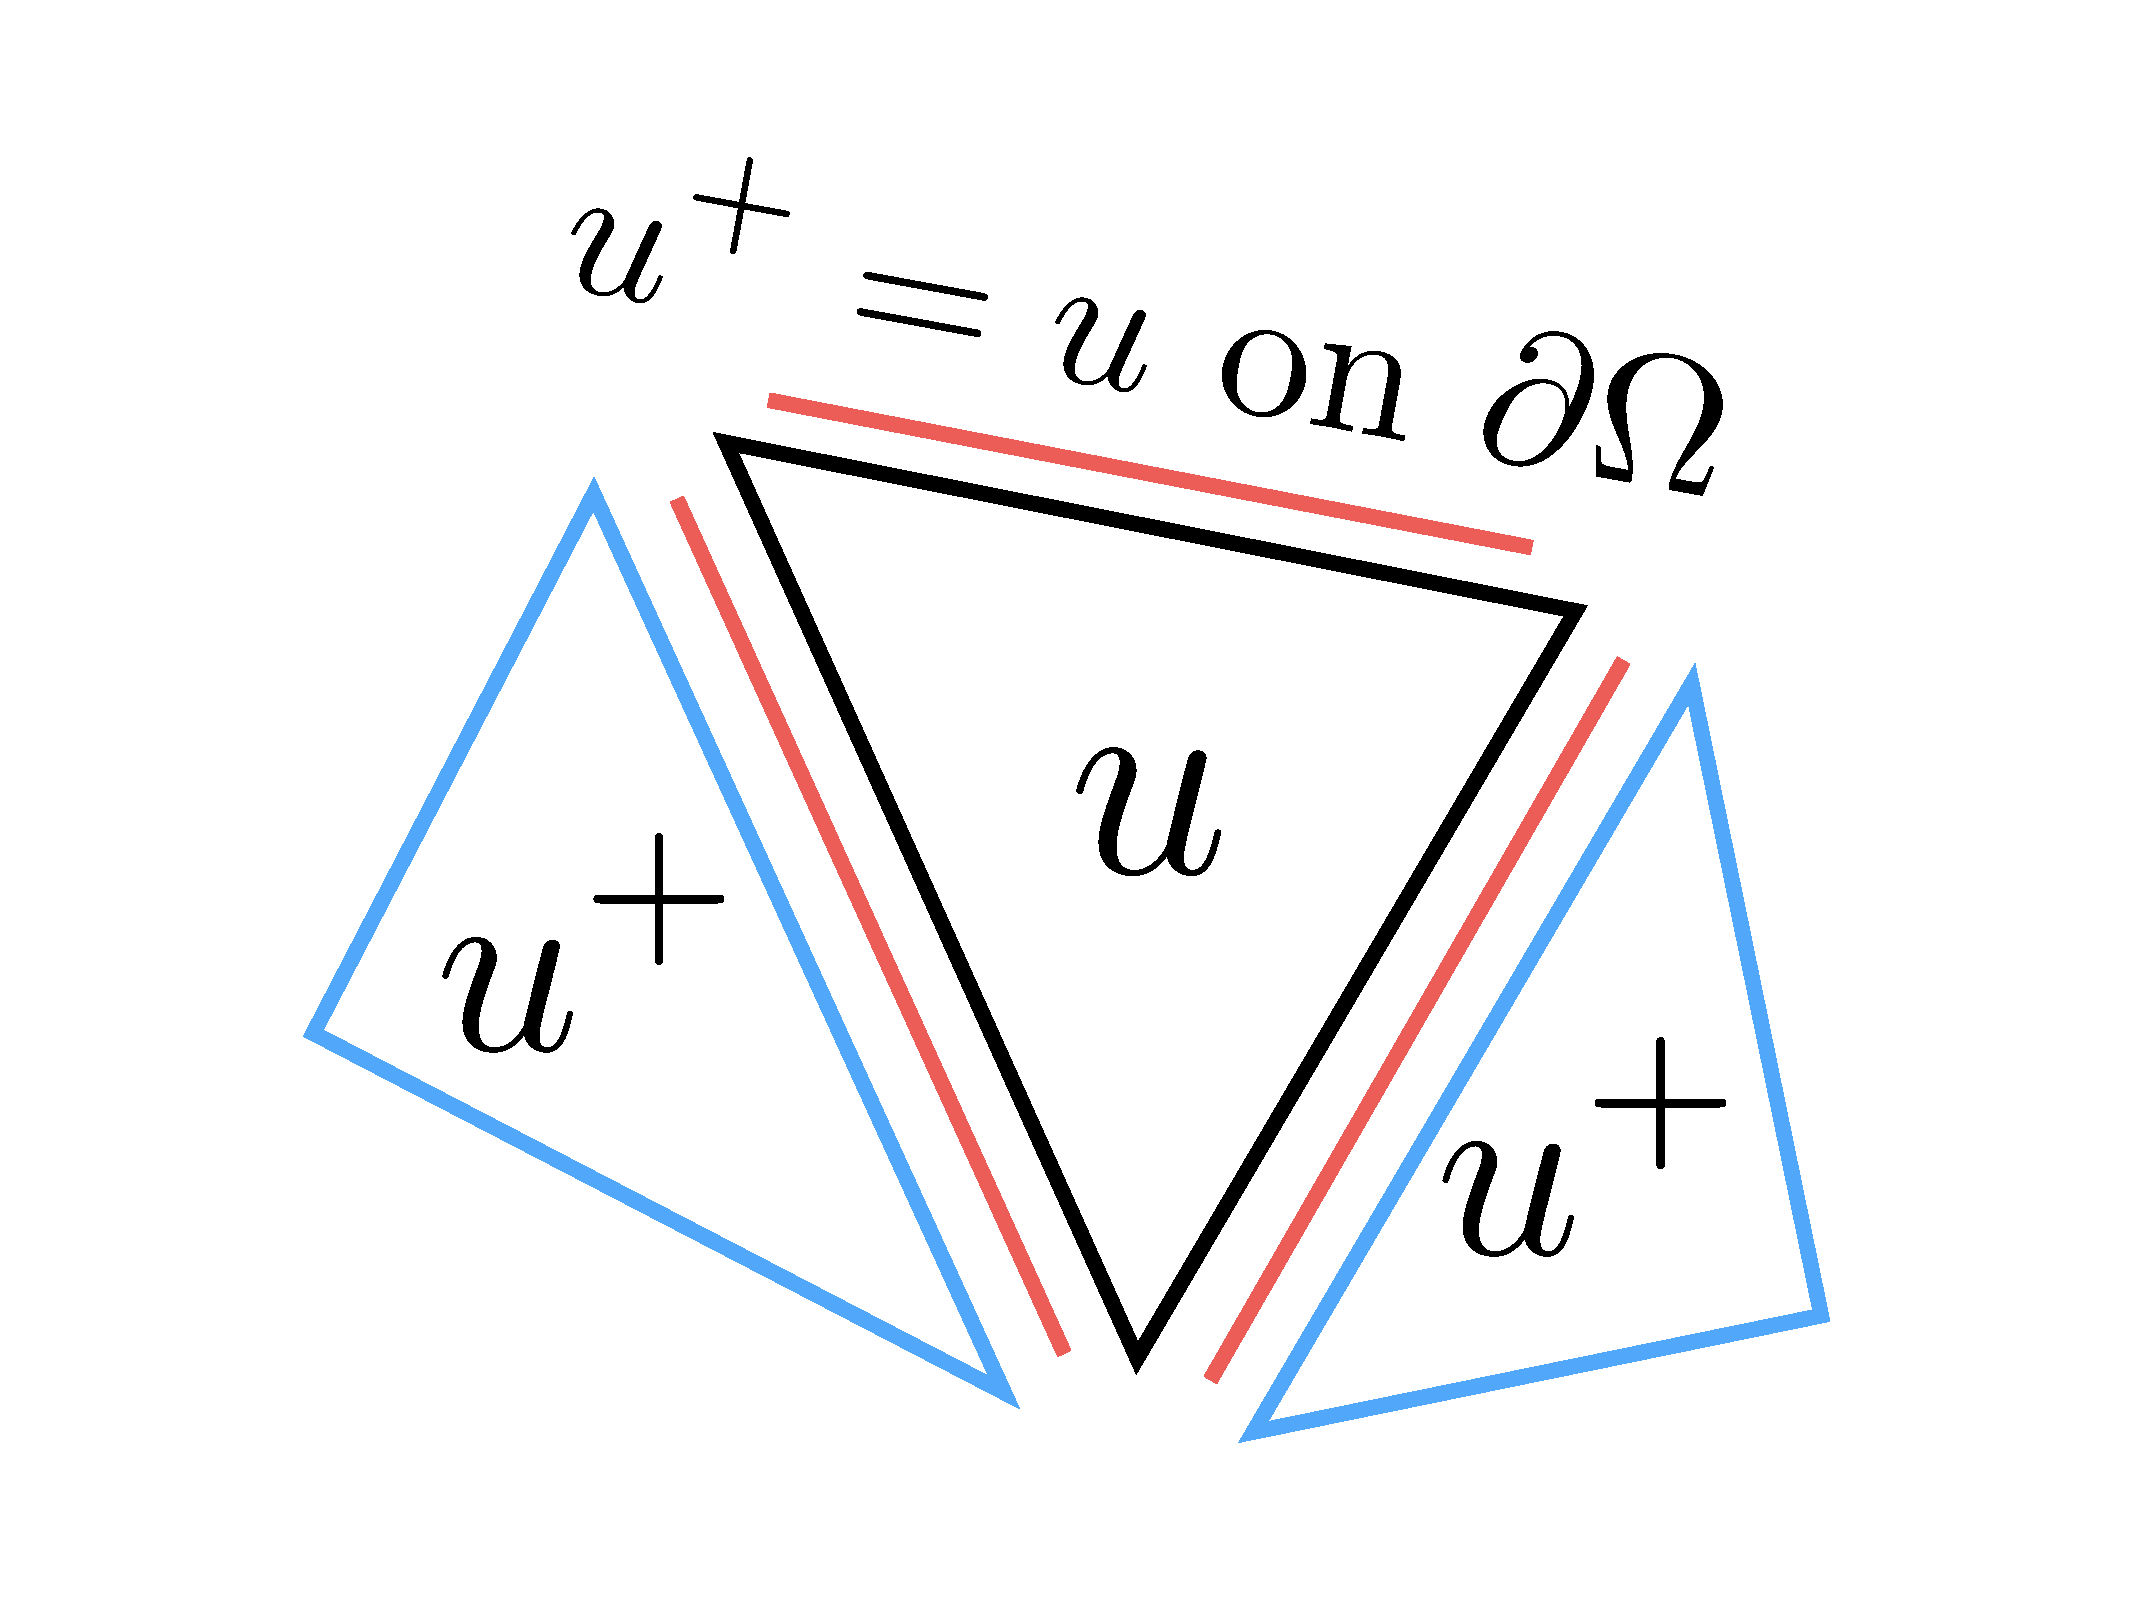
\includegraphics[width=.475\textwidth]{figs/jumpAvg.pdf}}
%\end{figure}
%}
%\only<2->{
%\item<2-> Affine meshes: define \note{global} DG derivative $D^x_h: V_h \rightarrow V_h$: $\forall v\in V_h$, 
%\begin{align*}
%\LRp{D^x_h u,v}_{\Omega} &= \sum_{k} \LRp{-u,\pd{v}{x}}_{D^k} + \LRa{\avg{u},vn_x}_{\partial D^k},\\ 
%&= \sum_{k} \LRp{\pd{u}{x},v}_{D^k} + \frac{1}{2}\LRa{\jump{u},vn_x}_{\partial D^k}.  
%\end{align*}
%\item<3-> Global integration by parts: {holds for quadrature (degree $\geq 2N-1$)}. 
%\[
%\LRp{D^x_h u,v}_{\Omega} = \LRa{ u,v n_x}_{\partial \Omega} - \LRp{u, D^x_hv}_{\Omega}, \qquad \forall u,v \in V_h.
%\]
%}
%\end{itemize}
%\end{overlayarea}
%}
%
%\frame{
%\frametitle{Global DG differentiation matrices}
%\begin{itemize}
%\item $D^x_h$ a matrix representation
%\item Let $\bm{U} = [\bm{u}_1,\ldots,\bm{u}_K]^T$.  Semi-discrete system: 
%\[
%\td{\bm{U}}{t} = \bm{D}^x_h \bm{U}
%\]
%\end{itemize}
%}
%
%\frame{
%\frametitle{DG energy estimates for linear advection }
%
%\begin{itemize}
%\item Advection formulation: positive semi-definite penalization $s_\tau(u,v)$
%\[
%\LRp{\pd{u}{t} + D^x_h u,v}_{\Omega} + \underbrace{\sum_{k} \LRa{-\tau\frac{\LRb{n_x}}{2} \jump{u},v}_{\partial D^k}}_{s_\tau(u,v) } = 0. %\text{, pos.\ semi-def.}
%\]
%\item Energy method: take $v = u$, integrate by parts.  
%\begin{align*}
%&\LRp{\pd{u}{t},u} + \frac{1}{2}\note{{\LRp{2D^x_h u,u}_{\Omega}}} + s_{\tau}(u,u) = 0.  \\
%&\note{\LRp{2D^x_h u,u}_{\Omega}} = {\LRp{D^x_h u,u}_{\Omega} + \LRa{u,un_x}_{\partial \Omega} - \LRp{u,D^x_h u}_{\Omega}},\\
%&\Longrightarrow \frac{1}{2}\pd{}{t}\nor{u}^2_{L^2\LRp{\Omega}} +  \frac{1}{2}\LRa{u,un_x}_{\partial \Omega} = -s_{\tau}(u,u) \leq 0.
%\end{align*}
%
%\end{itemize}
%}


%% =================================================


\frame{
\frametitle{Generalization to nonlinear problems: entropy stability}
\vspace{-.5em}
\begin{itemize}
\item Generalizes energy stability to \note{nonlinear} systems of conservation laws (Burgers', shallow water, compressible Euler, MHD).  
\[
\pd{\bm{u}}{t} + \pd{\bm{f}(\bm{u})}{x} = 0.  
\]
\item Continuous entropy inequality: given a convex \note{entropy} function $S(\bm{u})$ and ``entropy potential'' $\psi(\bm{u})$, 
\begin{align*}
&\int_{\Omega} \bm{v}^T\LRp{\pd{\bm{u}}{t} + \pd{\bm{f}(\bm{u})}{x}} = 0, \qquad \bm{v} = \pd{S}{\bm{u}} \\
&\Longrightarrow \int_{\Omega}\pd{S(\bm{u})}{t} + \LRu{\LRp{\bm{v}^T\bm{f}(\bm{u}) - \psi(\bm{u})}}_{-1}^1 \leq 0.
\end{align*}
\vspace{.01em}
\item Proof of entropy inequality relies on \note{chain rule}, integration by parts.  
\end{itemize}
}

%\frame{
%\frametitle{Example: compressible flow and mathematical entropy}
%
%\begin{itemize}
%\item Conservative variables: density, momentum, energy
%\[
%\bm{u} = (\rho, \bm{m}, E), \qquad \rho > 0, \qquad E > \frac{1}{2} {\LRb{\bm{m}}^2}/{\rho}.
%\]
%\item Physical entropy $s(\bm{u})$ always increasing; \note{mathematical entropy $S(\bm{u})$} always decreasing (analogous to energy).
%\[
%s(\bm{u}) = \log\LRp{\frac{(\gamma-1) \rho e}{\rho^\gamma}}, \qquad S(\bm{u}) = -\rho s(\bm{u}).
%\]
%\item Entropy variables $\bm{v}(\bm{u})$: invertible function of $\bm{u}$
%\[
%\bm{v}(\bm{u}) = \pd{S}{\bm{u}} = \frac{1}{\rho e} \LRp{\begin{array}{c}
%\rho e (\gamma + 1 - s(\bm{u})) - E \\
%m\\
%-\rho
%\end{array}}
%\]
%\end{itemize}
%}


\frame{
\frametitle{Why are discretizations of nonlinear PDEs unstable?}
\setcounter{subfigure}{0}
\vspace{-1em}
\begin{figure}
\begin{overprint}
\centering
\foreach \id in {1,2,3,4}{%
\only<\id>{
\captionsetup[subfloat]{width=.45\textwidth, justification=centering}
\subfloat[Exact solution]{%[$N = 7, K = 8$ (aligned mesh)]{
\makebox[.425\textwidth]{\includegraphics[width=.32\textwidth]{figs/burgersStable_\id.png}}}%
\hspace{1em}%
\subfloat[8th order DG]{ %[$N = 7, K = 9$ (non-aligned mesh)]{
\makebox[.425\textwidth]{\includegraphics[width=.32\textwidth]{figs/burgersUnstable_\id.png}}}
} % only
} % foreach 
\end{overprint}
\end{figure}
\vspace{-.5em}
\begin{itemize}
\item Burgers' equation: $f(u) = u^2/2$.  How to compute $\pd{}{x}f({u})$?  
\[
\pd{u}{t} + \frac{1}{2}\pd{u^2}{x} = 0, \qquad u \in P^N(D^k), \quad u^2 \not\in P^N(D^k).
\]
\item Differentiating $L^2$ projection $P_N$ + inexact quadrature: \note{no chain rule}.  
\[
\int_{D^k}\LRp{\pd{u}{t} + \frac{1}{2} \pd{}{x} P_N u^2}v \diff{x} = 0, \qquad \frac{1}{2}\pd{P_N u^2}{x} \neq P_N \LRp{u \pd{u}{x}}
\]
\end{itemize}
}

\frame{
\frametitle{Tradeoff between high order accuracy vs stability}

\begin{overlayarea}{\textwidth}{.85\textheight}
\begin{itemize}
\item<1-> \textcolor{red}{Asymptotic} stability for \textcolor{red}{smooth} solutions (not shocks or turbulence!)
\item<3-> Common fix: \note{stabilize by regularizing} (limiters, filters, art.\ viscosity).  
\end{itemize}
\begin{figure}
\centering
\only<1>{
\vspace{.5em}
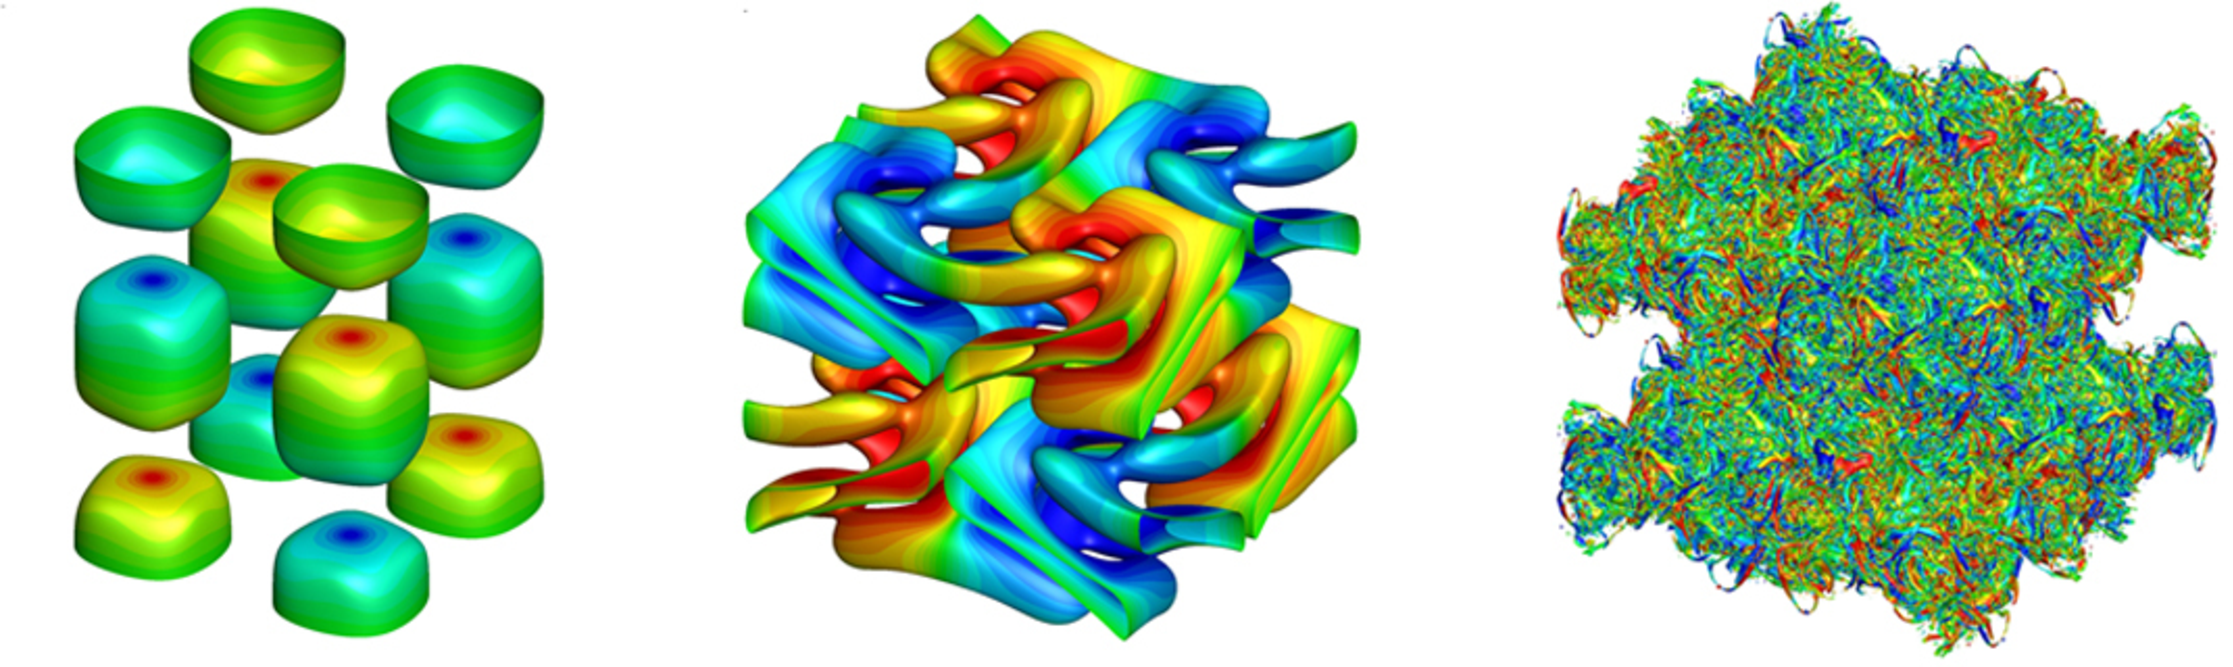
\includegraphics[width=1\textwidth]{figs/gassner_turb_01.pdf}
\caption*{Under-resolved solutions: turbulence (inviscid Taylor-Green vortex).}}
\only<2>{
\vspace{-.5em}
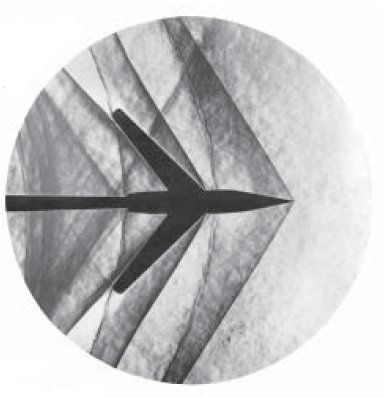
\includegraphics[width=.35\textwidth]{figs/shadowgraph.jpg}
\hspace{1em}
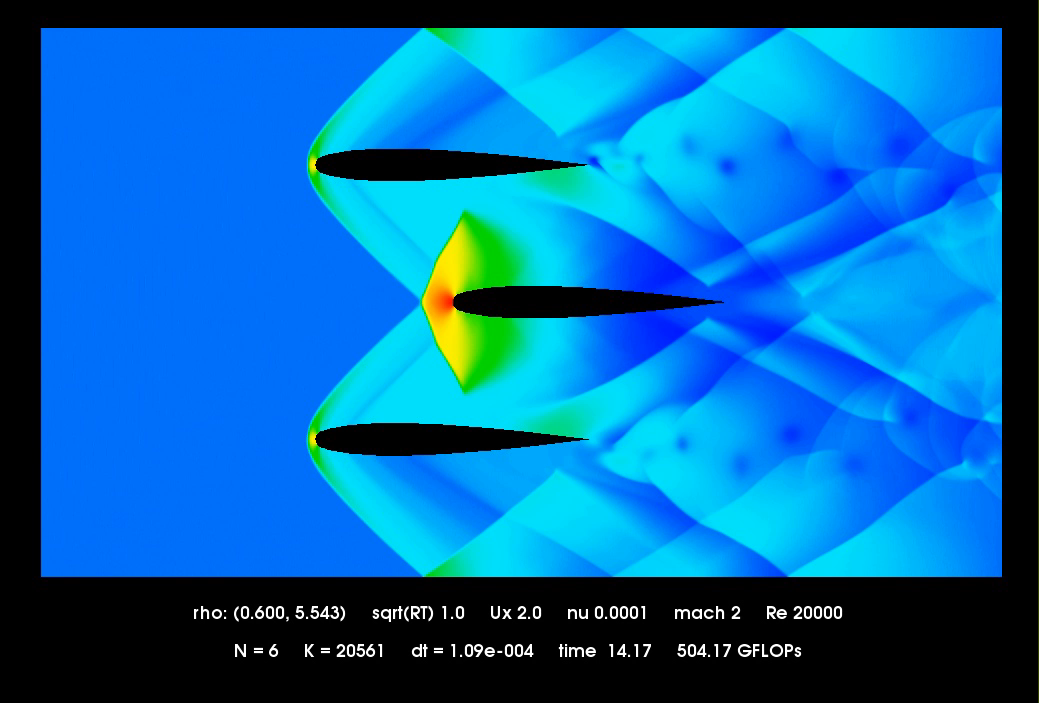
\includegraphics[width=.5\textwidth]{figs/trifoil.png}
\caption*{Under-resolved solutions: shock waves.}
}
\only<3>{
\vspace{1em}
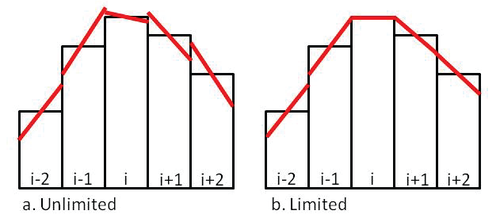
\includegraphics[width=.675\textwidth]{figs/slopeLimit.png}
\caption*{Slope limiting for a finite volume method.}
}
\only<4->{
\vspace{-1em}
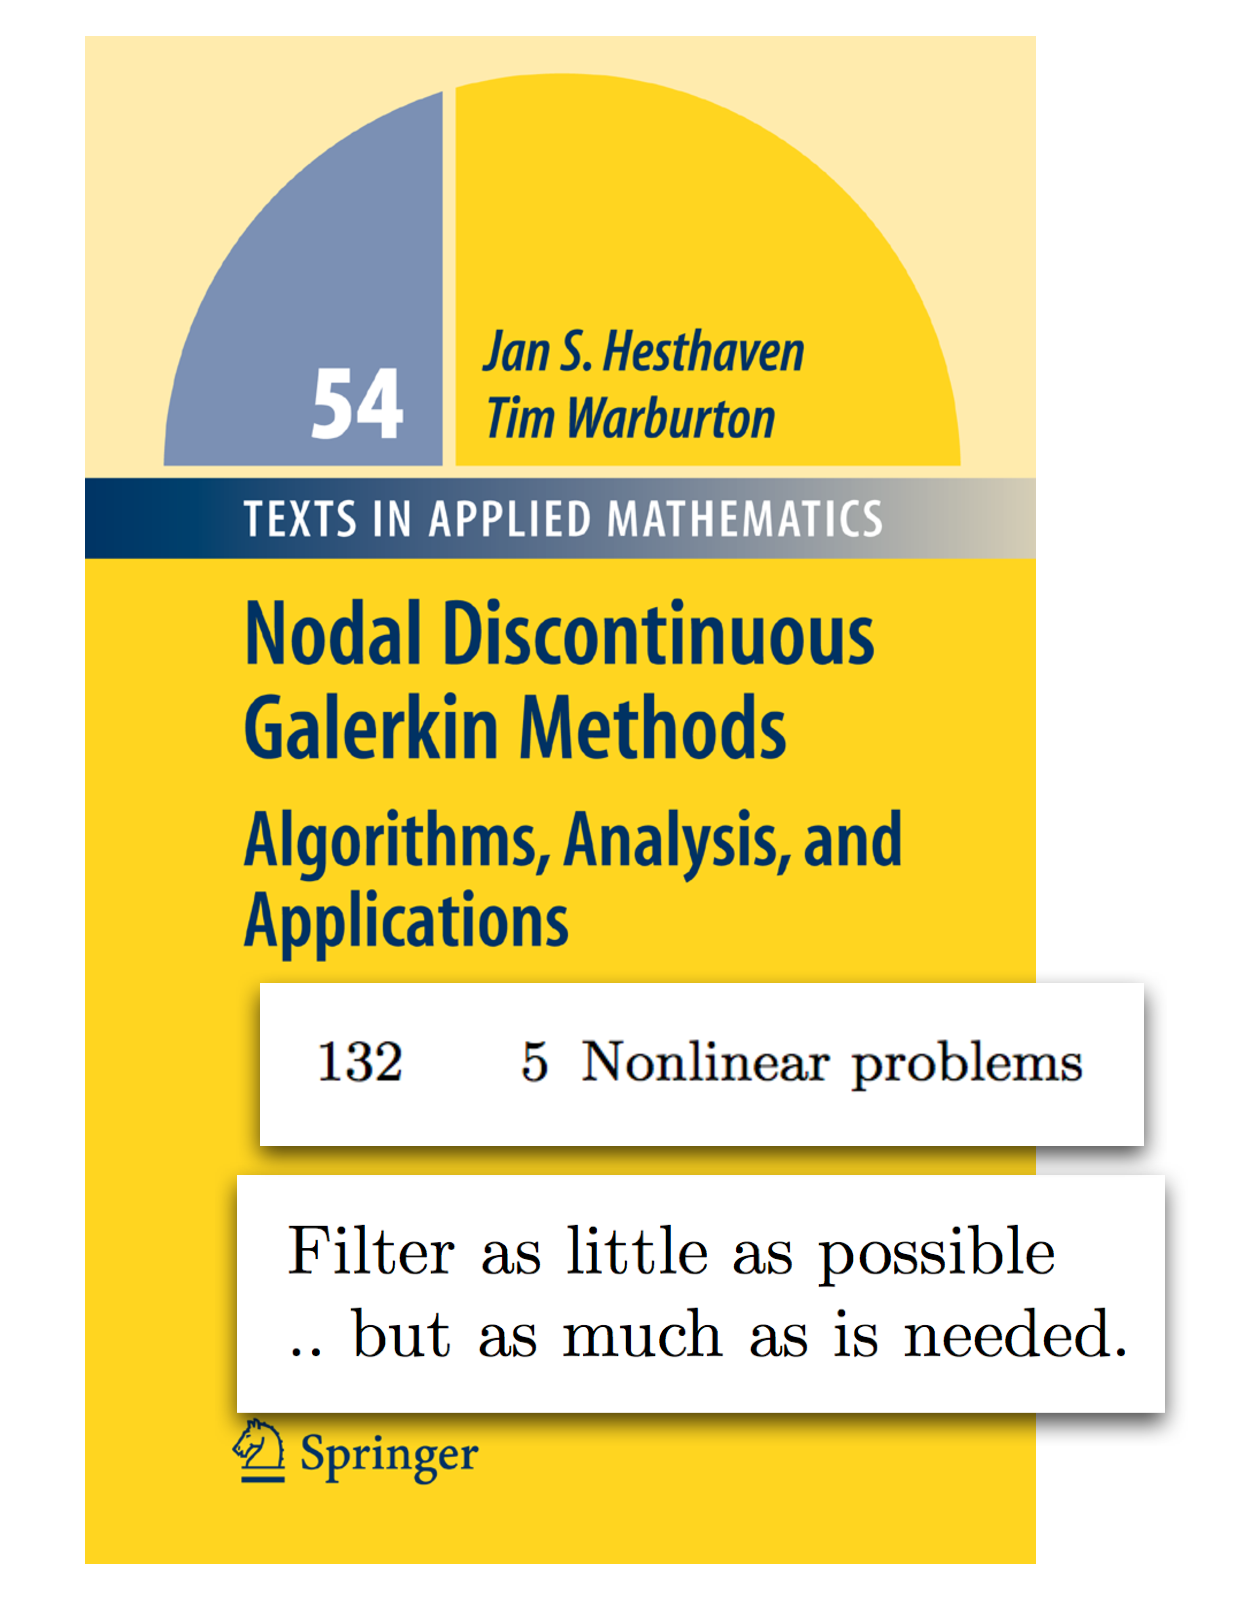
\includegraphics[width=.38\textwidth]{figs/ndgFilter.pdf}
\hspace{1em}
\visible<5>{\raisebox{2.5em}{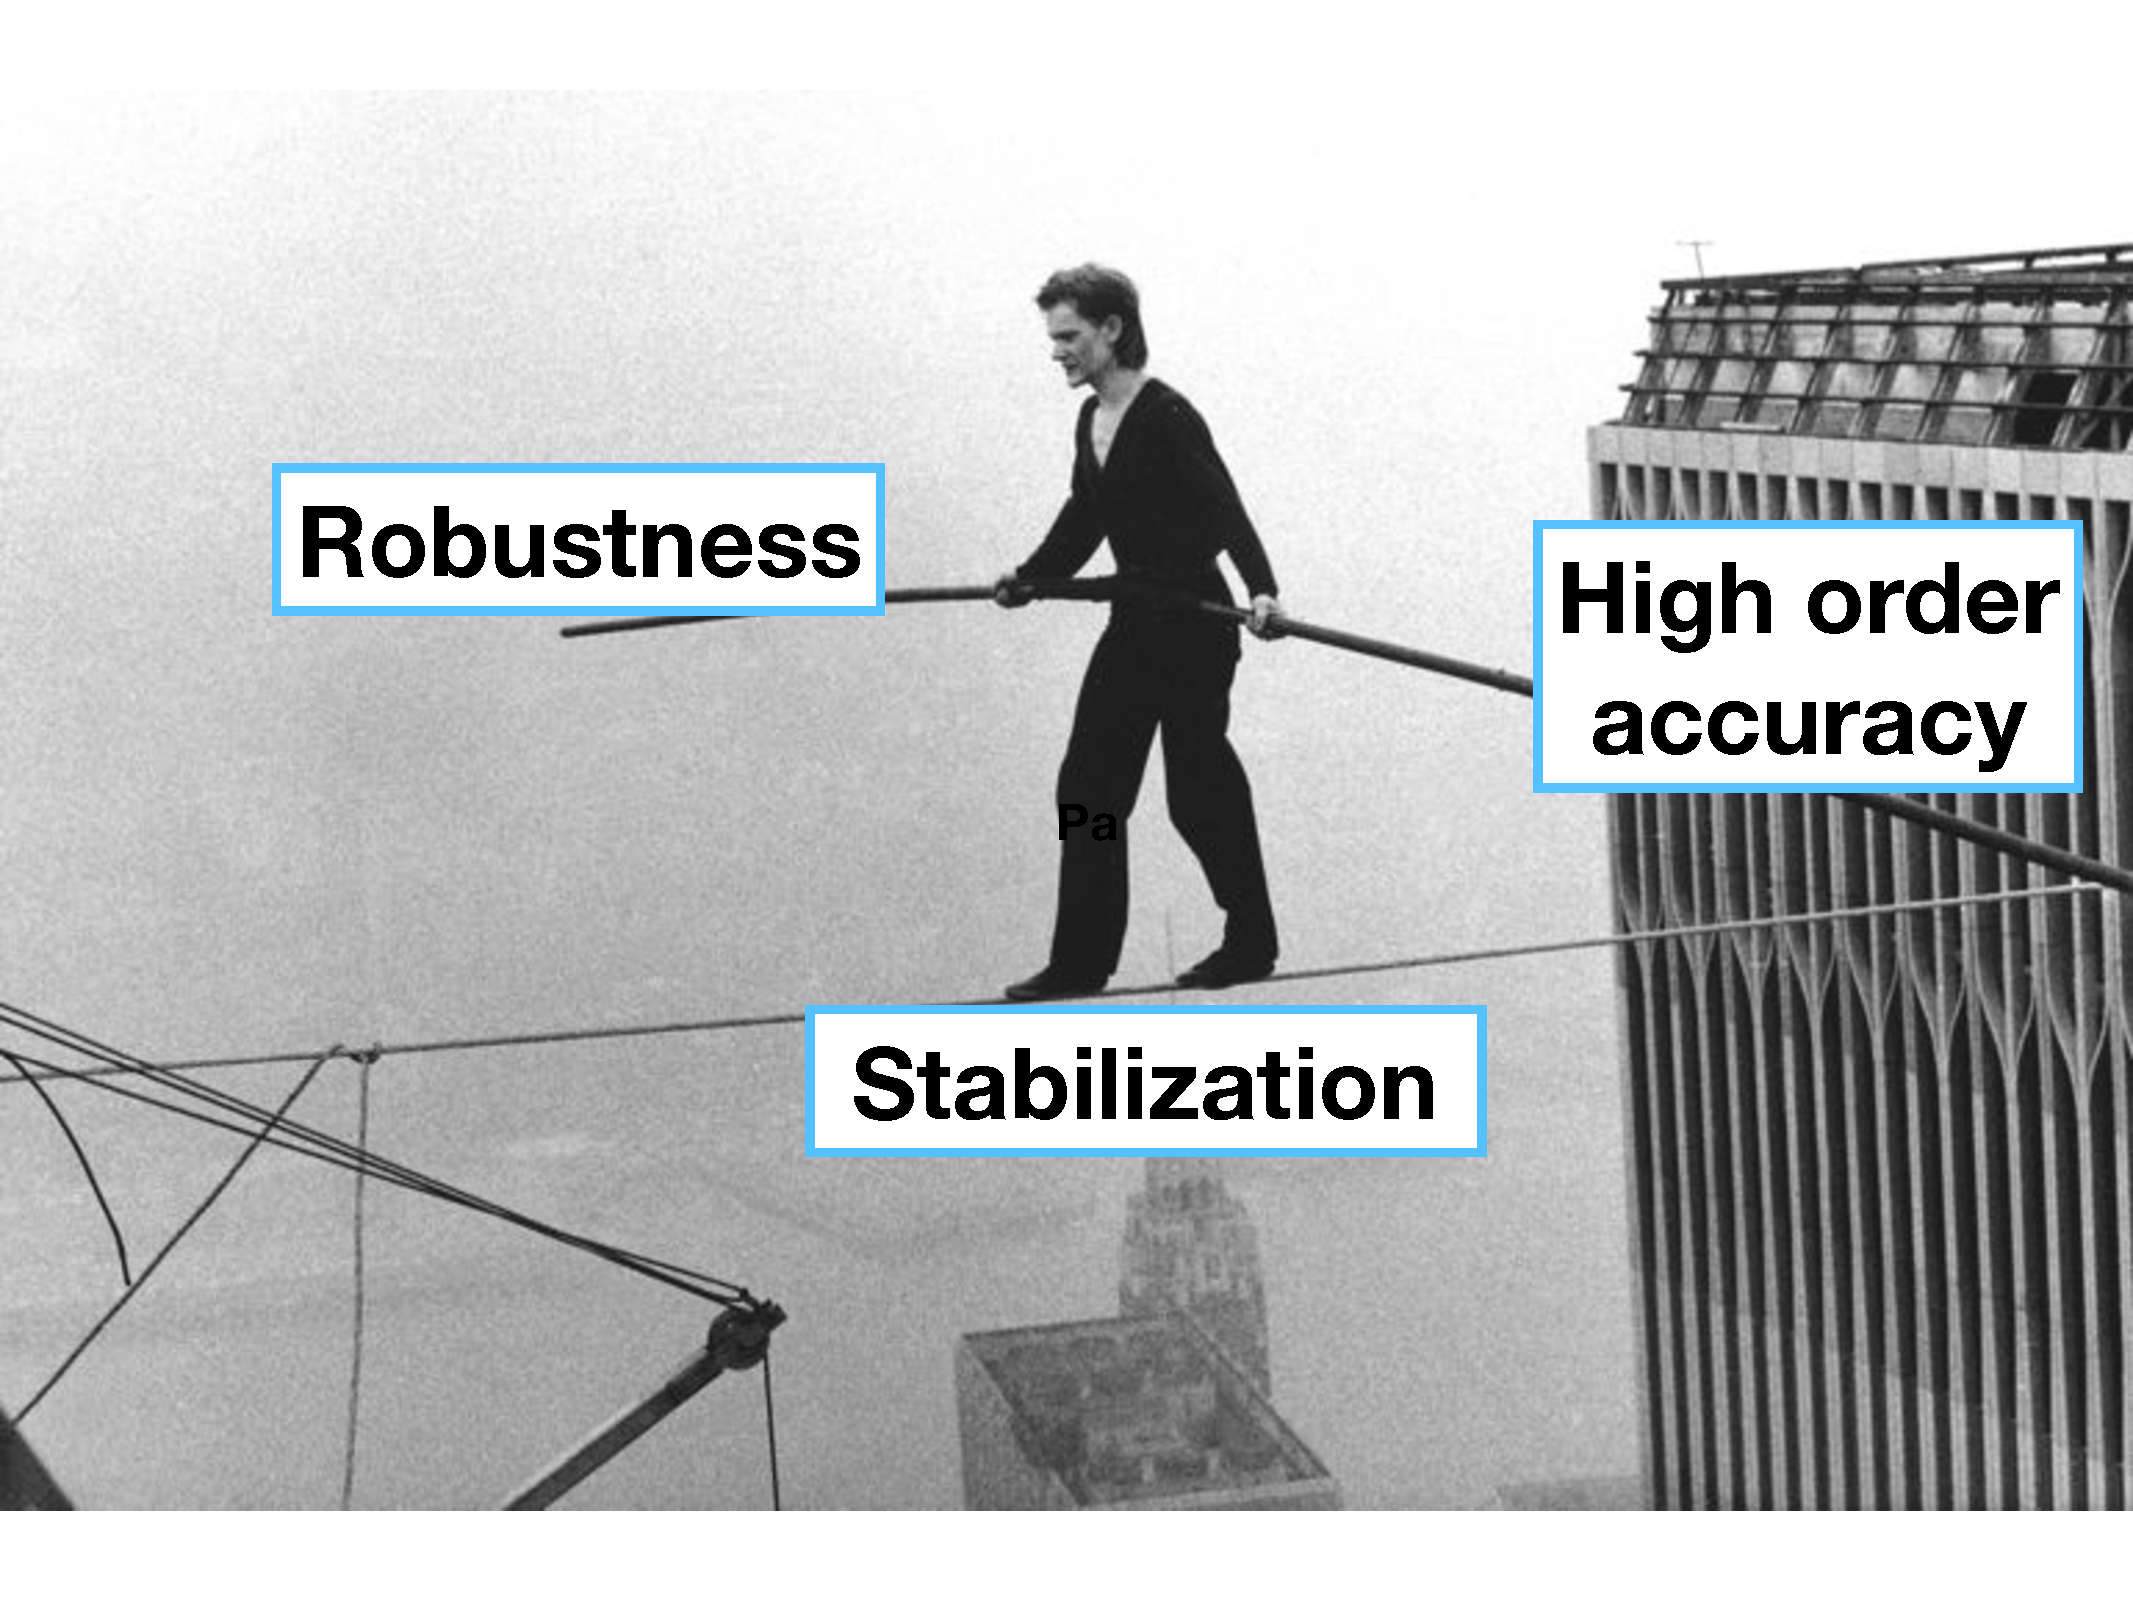
\includegraphics[width=.49\textwidth]{figs/balancing.pdf}}}
%\visible<5>{
\includegraphics[width=.475\textwidth]{figs/ductTape.png}}
}
\end{figure}
\end{overlayarea}
\let\thefootnote\relax\footnotetext{\tiny Figures courtesy of \href{http://www.gauss-centre.eu/gauss-centre/EN/Projects/CSE/2014/gassner_turbulence.html?nn=1345710}{Gregor Gassner}, T.\ Warburton, \href{http://cirpwiki.info/wiki/CMS-Flow_Numerical_Methods}{Coastal Inlets Research Program (CIRP)}, ``Man on Wire'' (2008).}
}

%% =================================================

%\section{Entropy stable formulations} 
%

\section{Summation-by-parts and high order DG}

\frame[noframenumbering]{
\frametitle{Talk outline}
\tableofcontents[currentsection]
}

\frame{
\frametitle{Nodal DG and summation-by-parts (SBP) in 1D}
\setcounter{subfigure}{0}

\vspace{-.75em}
\begin{figure}
\centering
%\begingroup
%\captionsetup[subfloat]{width=.475\textwidth}
%\subfloat[Higher order SBP matrix]{\raisebox{0em}{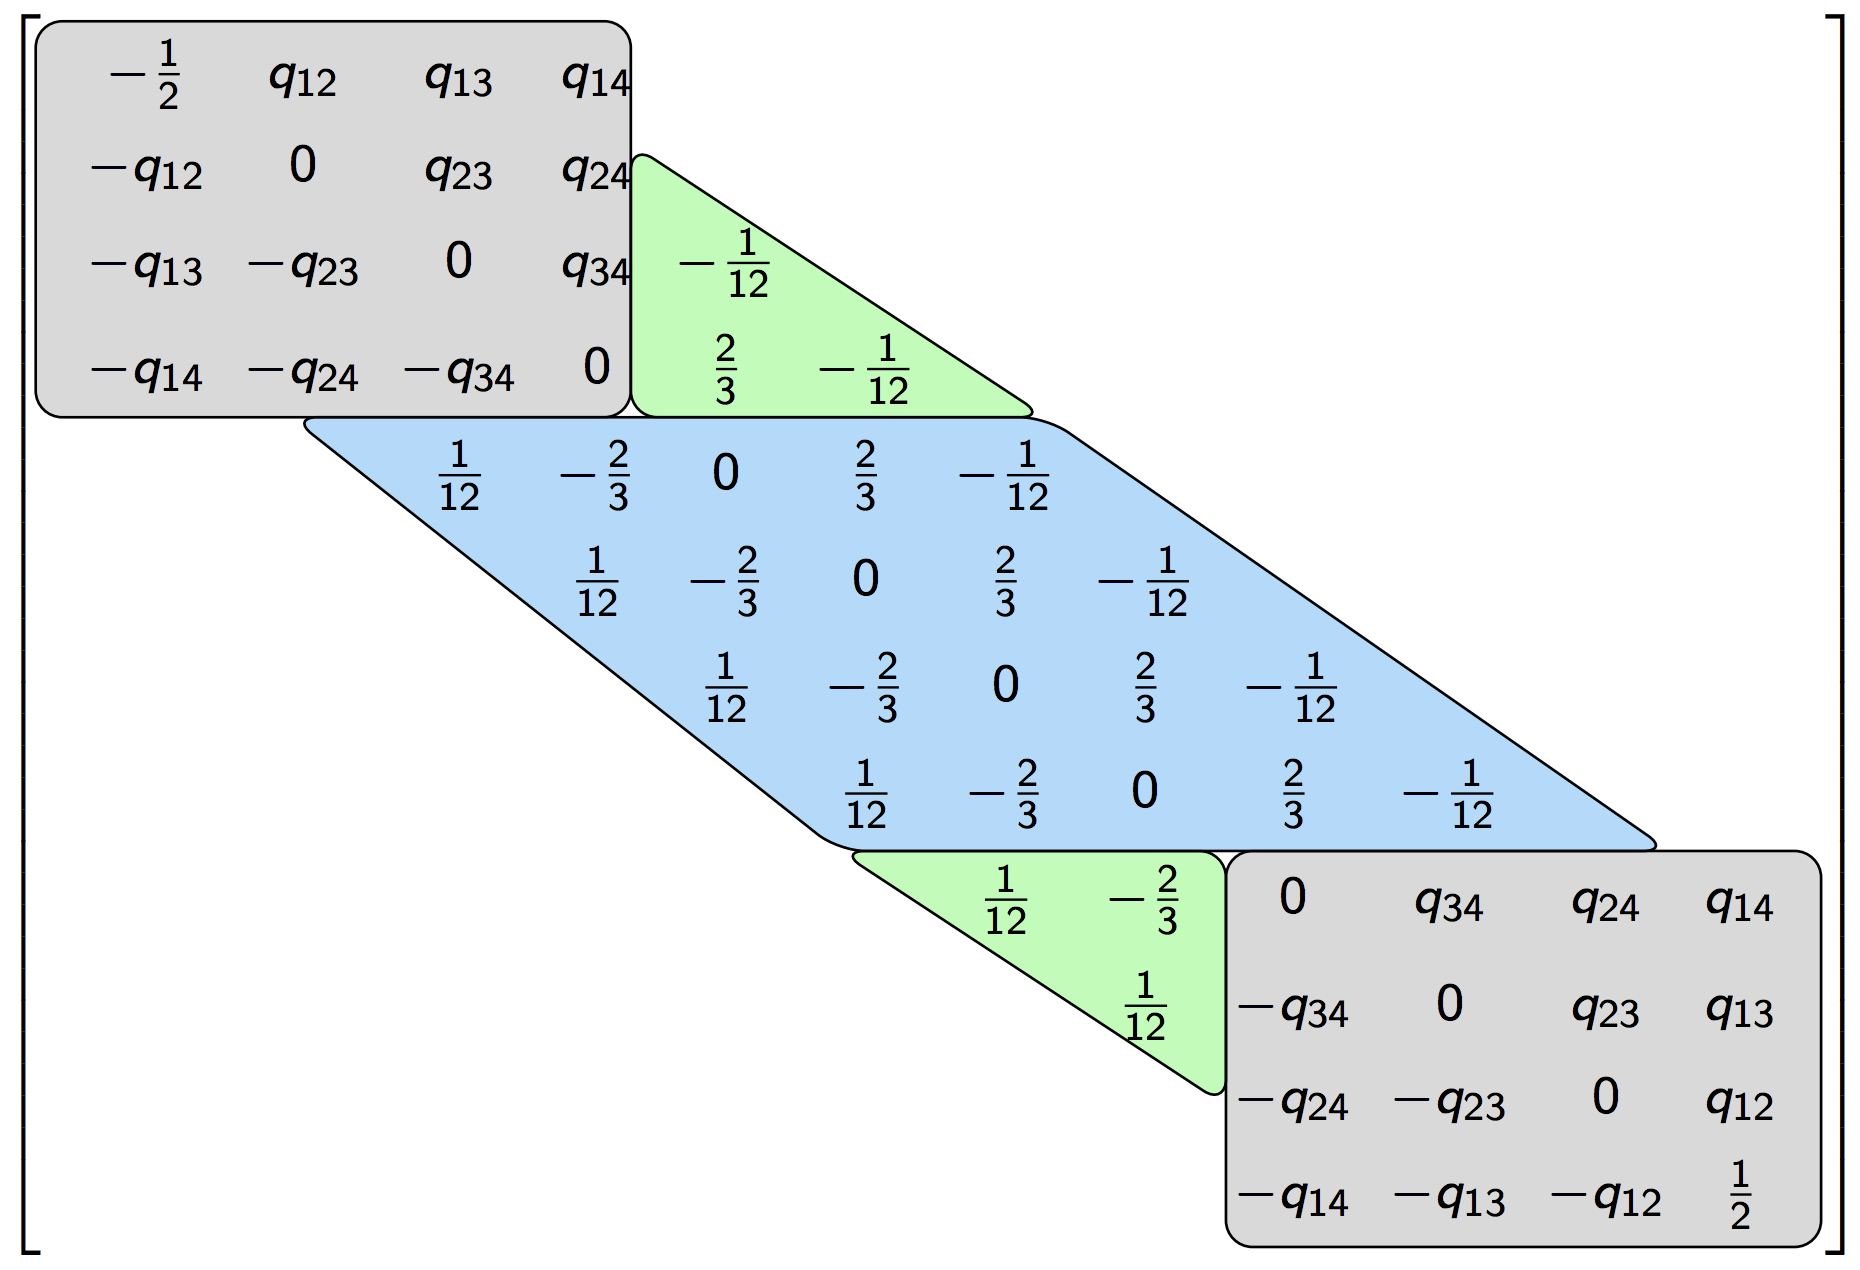
\includegraphics[width=.4\textwidth]{figs/sbp_dcdr.png}}}
%\hspace{1em}
%\subfloat[1D SBP ($N=7$, GLL nodes)]{
\subfloat{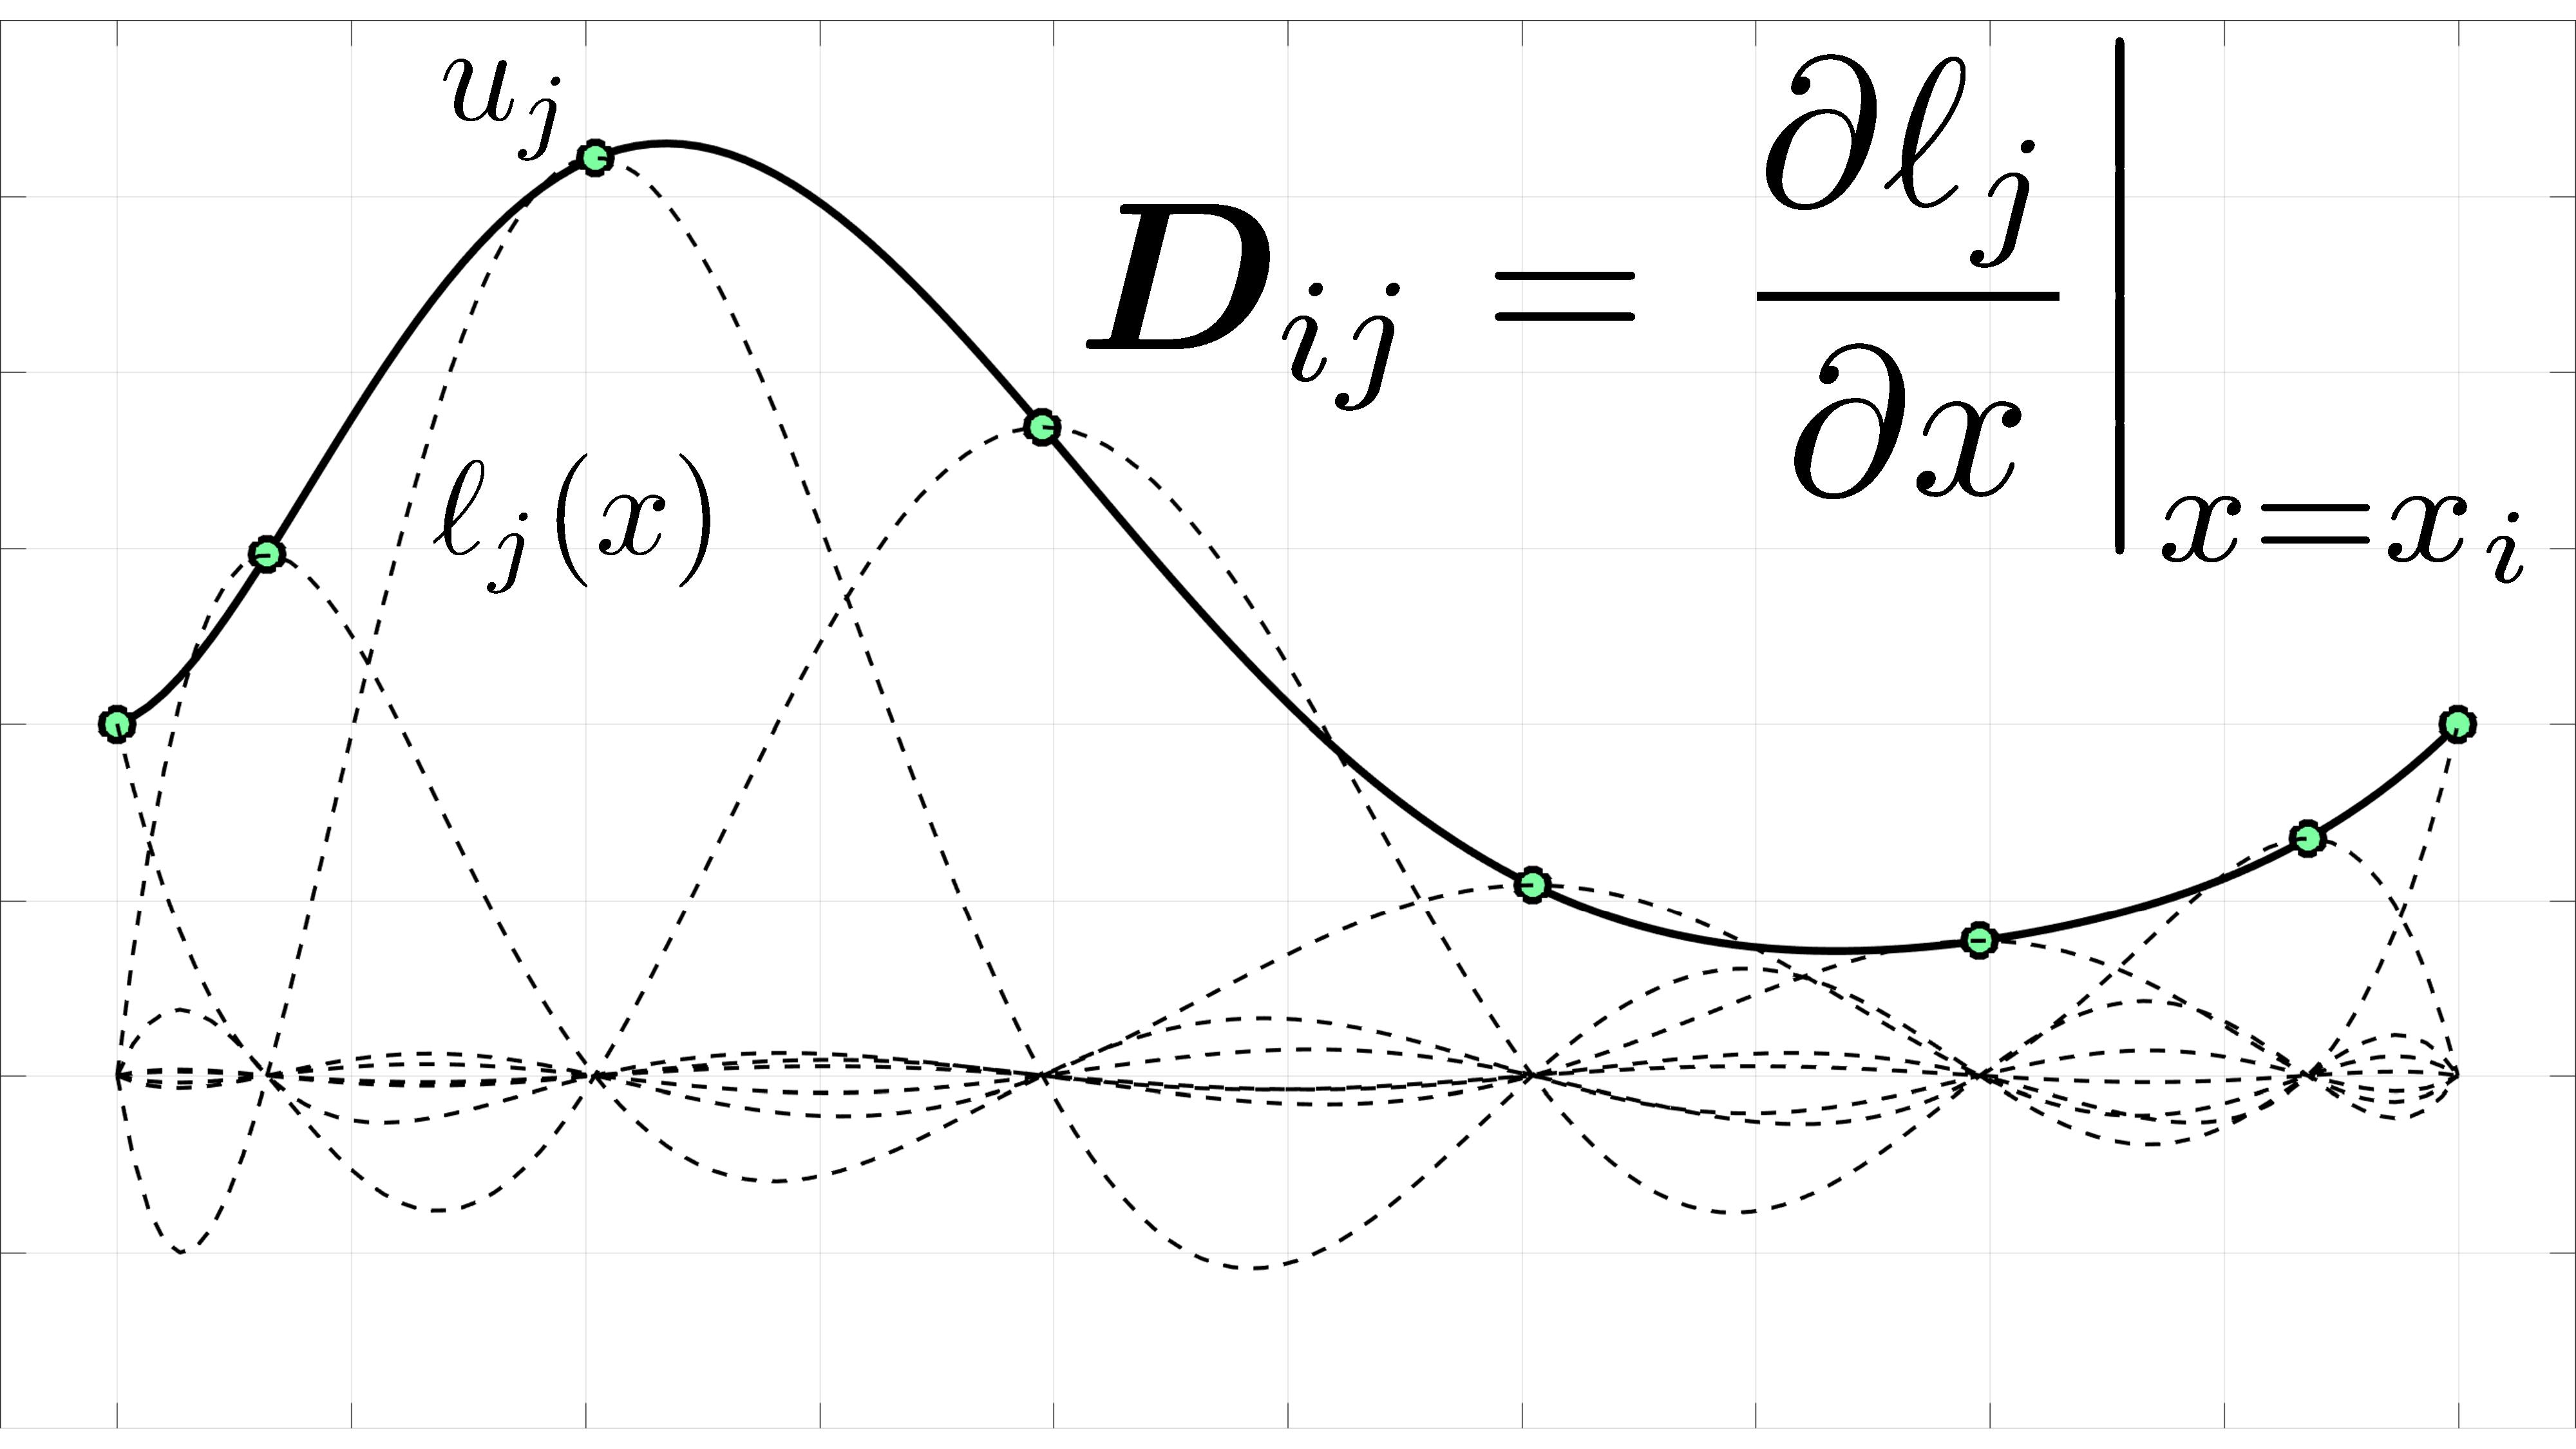
\includegraphics[width=.49\textwidth]{figs/gll1Dsbp.pdf}}
\hspace{1.5em}
\subfloat{\raisebox{1em}{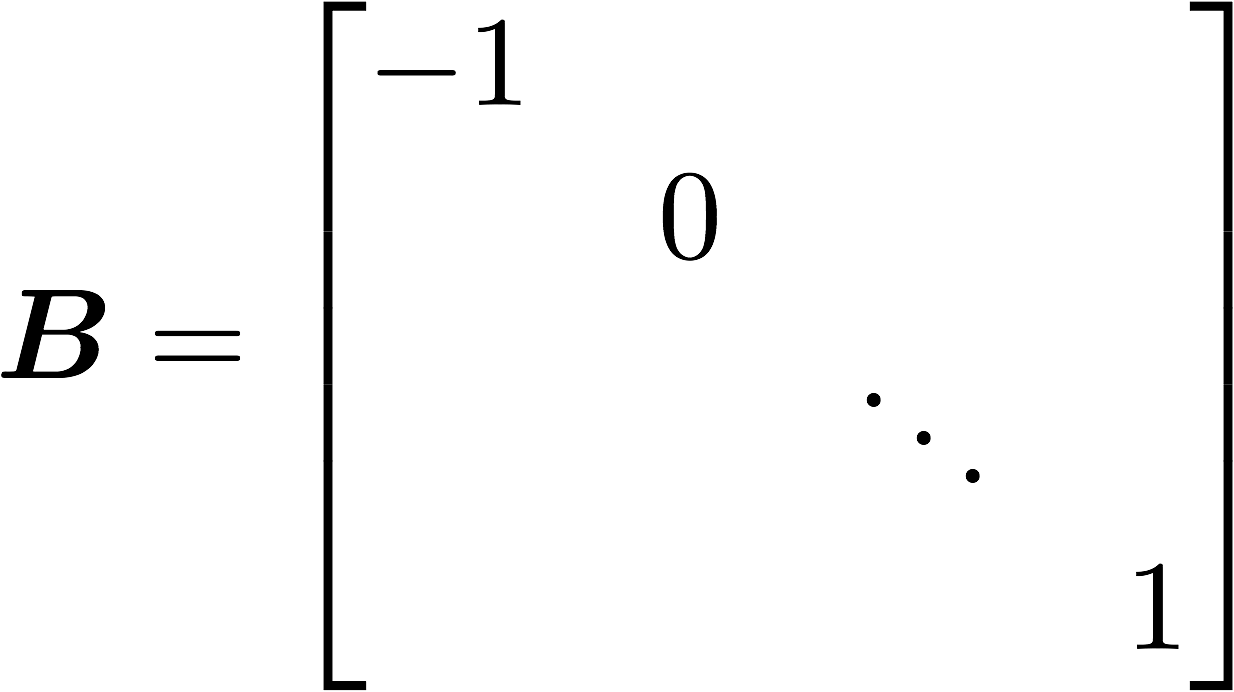
\includegraphics[width=.375\textwidth]{figs/B_SBP.png}}}
%}
%\subfloat[2D SBP ($N=7$, GLL nodes)]{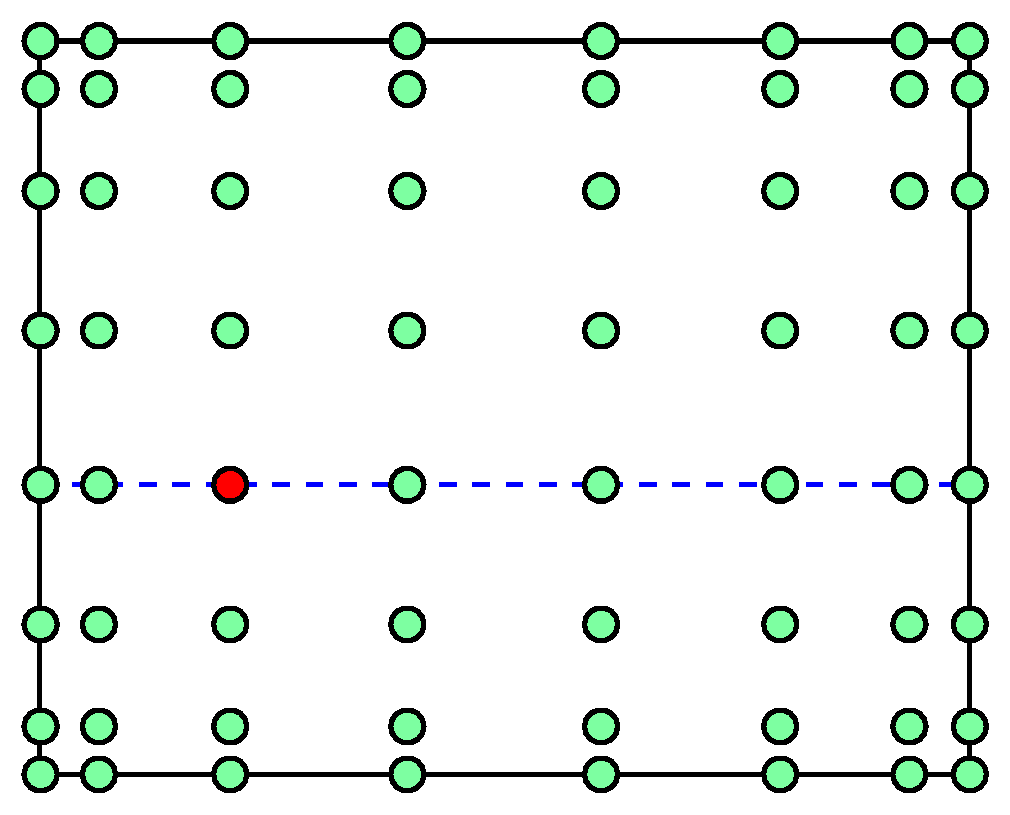
\includegraphics[width=.39\textwidth]{figs/SEM_stencil_1.pdf}}
%\subfloat[Diag-norm SBP nodes ($N=4$, 22 pts)]{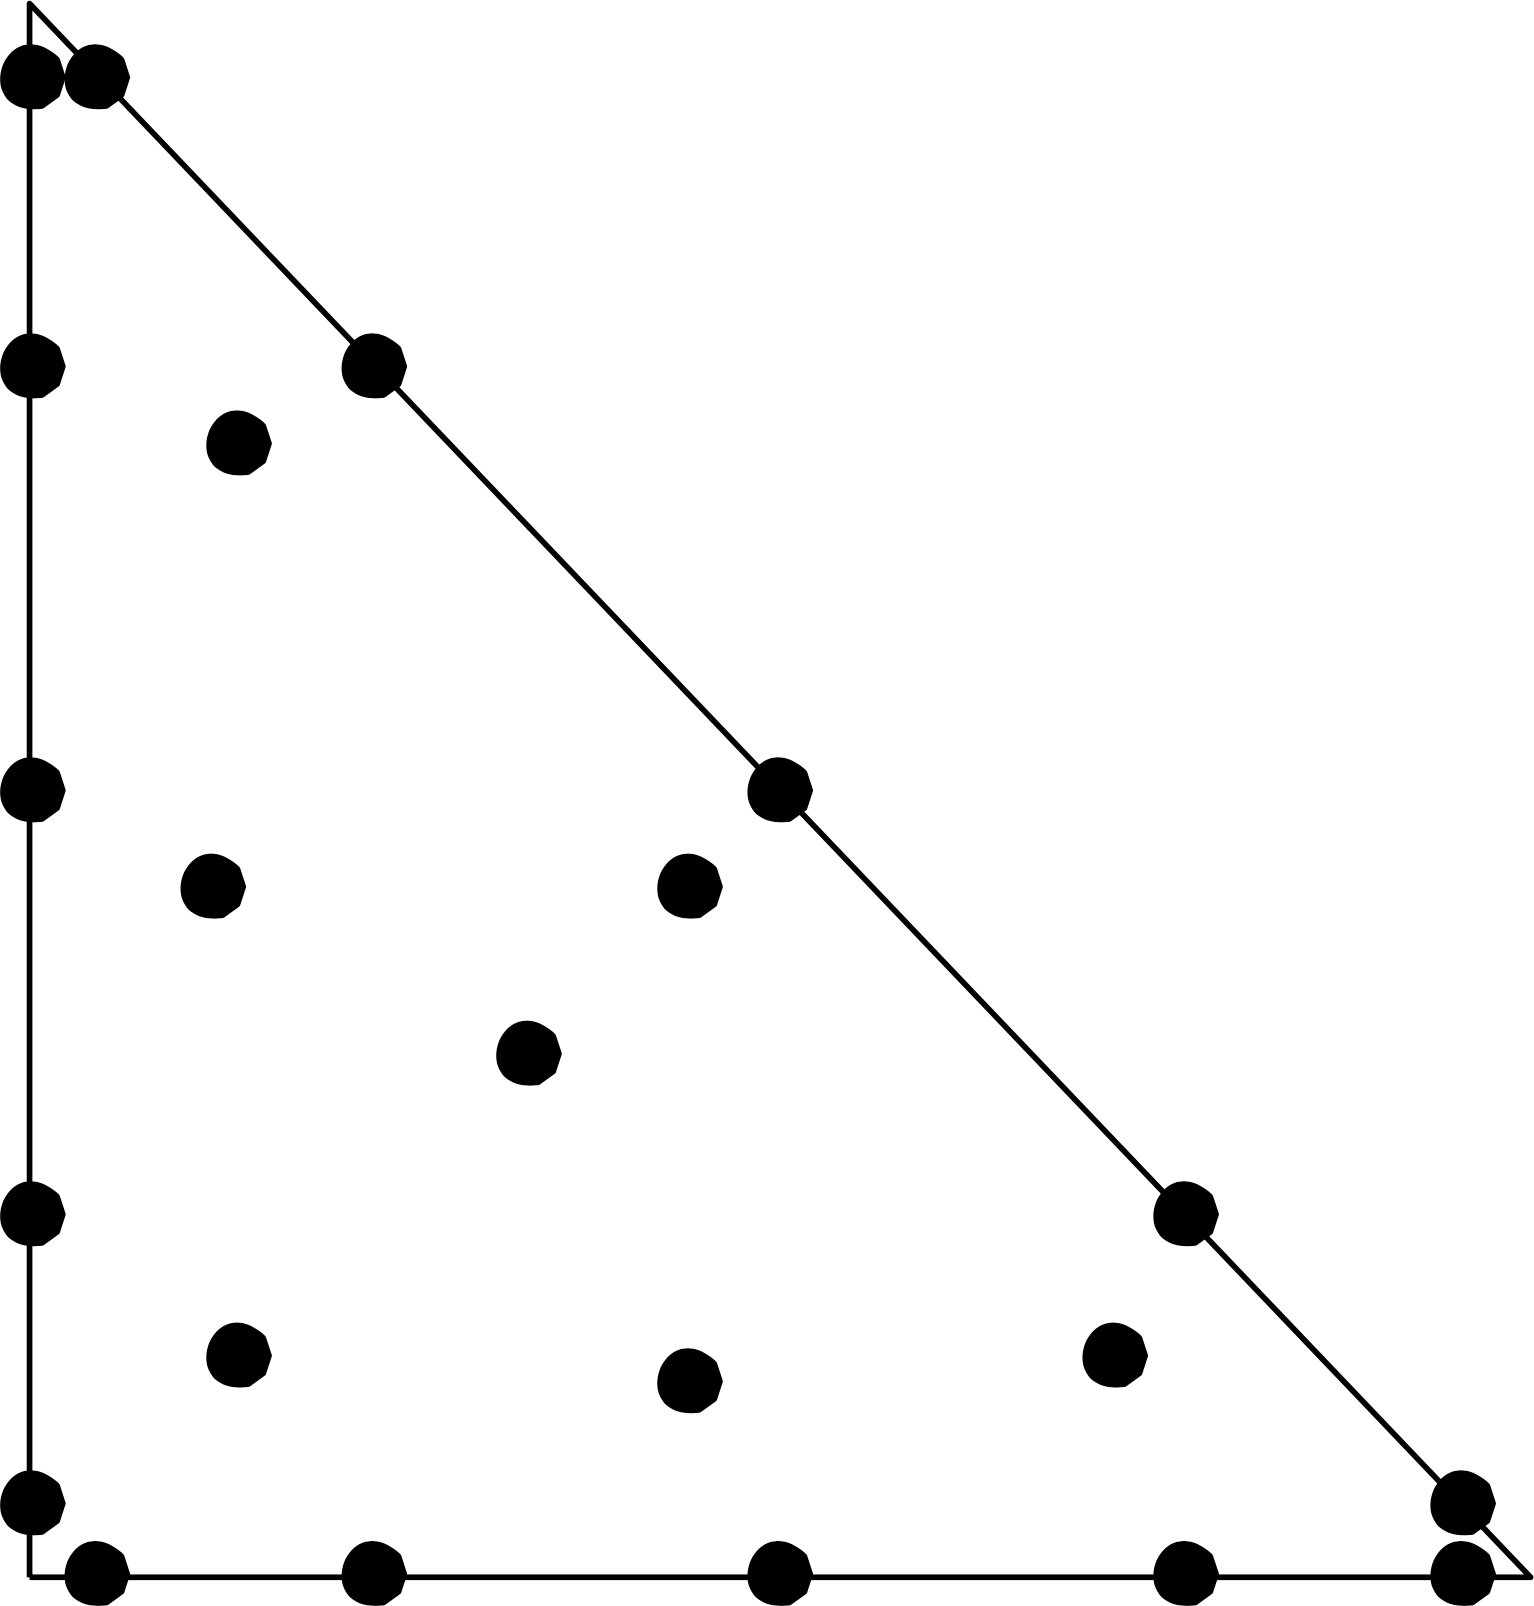
\includegraphics[height=.33\textheight]{figs/chenShuNodes.png}}
%\endgroup
%\caption{Dif.}
\end{figure}
\vspace{-.25em}
\begin{itemize}
%\item Solve for high order ``diagonal-norm'' SBP finite difference matrices.
%\vspace{.25em}
\item Gauss-Legendre-Lobatto (GLL) \note{quadrature} + \note{nodal basis}.
\vspace{.25em}
\item Mimic \note{integration by parts} algebraically using differentiation matrix $\bm{D}$, diagonal (lumped) mass matrix $\bm{M}$, and boundary matrix $\bm{B}$
\[
\bm{Q} = \bm{B} - \bm{Q}^T, \qquad \bm{Q} = \bm{M}\bm{D}, \qquad \bm{M} \text{ diagonal}.%, \qquad \bm{B} = \begin{bmatrix}
%-1 & &\\
%& \ddots &\\
%& & 1
%\end{bmatrix}
\]
%\item Nodal DG construction of diagonal-norm SBP matrices: Gauss-Legendre-Lobatto \note{quadrature} + \note{nodal basis} + \note{mass lumping}.  
%\item High order accuracy and provable \note{discrete stability}.
\end{itemize}

\let\thefootnote\relax\footnotetext{\tiny Gassner (2013). \textit{A skew-symmetric DG-SEM discretization and its relation to SBP-SAT finite difference methods.}}
%\let\thefootnote\relax\footnotetext{\tiny Figure courtesy of David C.\ Del Rey Fernandez.}
%\let\thefootnote\relax\footnotetext{\tiny Fisher and Carpenter (2013). \textit{High-order ES finite difference schemes for nonlinear conservation laws: Finite domains.} }
%\let\thefootnote\relax\footnotetext{\tiny Gassner, Winters, and Kopriva (2016). \textit{Split form nodal DG schemes with SBP property for the comp.\ Euler equations.}}
%\let\thefootnote\relax\footnotetext{\tiny Chen and Shu (2017). \textit{ES high order DG methods with suitable quadrature rules for hyperbolic conservation laws.}}
%\let\thefootnote\relax\footnotetext{\tiny Crean, Hicken, et al.\ (2018). \textit{Entropy-stable SBP discretization of the Euler equations on general curved elements.}}
}

%\frame{
%\frametitle{Summation-by-parts (SBP) finite differences}
%
%%\vspace{-1em}
%\begin{figure}
%\centering
%\begin{tikzpicture}
%\begin{scope}[font=\footnotesize, x=.3cm]
%  \foreach \mypt in {0,2,...,\bound}{
%    \draw(\mypt,0)circle[radius=2pt];
%    \draw(-\mypt,0)circle[radius=2pt];
%  }
%  \draw(-\bound,0)--(\bound,0) node[pos=0,left]{};
%  \node(start)[at={(-\bound,0)},label=below:{$u_1$}]{};
%  \node[at={(-\bound+2,0)},label=below:{$u_{2}$}]{};  
%  \node(end)[at={(\bound,0)},label=below:{$u_{N+1}$}]{};
%  \node[at={(\bound-2,0)},label=below:{$u_{N}$}]{};  
%  \node[at={(-2,0)},label=below:{$u_{i-1}$}]{};  
%  \node[at={(0,0)},label=below:{$u_i$}]{};    
%  \node[at={(2,0)},label=below:{$u_{i+1}$}]{};  
%  \node[at={(-5,0)},label=below:{$\ldots$}]{};      
%  \node[at={(5,0)},label=below:{$\ldots$}]{};        
%\only<1>{
%  \filldraw[color=red, fill=red!50, very thick](0,0)circle[radius=2pt];
%  }
%\only<2>{
%  \filldraw[color=red, fill=red!50, very thick](-\bound,0)circle[radius=2pt];
%  \filldraw[color=red, fill=red!50, very thick](\bound,0)circle[radius=2pt];  
%  }
%\end{scope}
%\end{tikzpicture}
%\caption*{Simplest SBP finite difference matrix: combine 2nd order finite difference formulas at interior points with 1st order finite differences at boundary points .}
%\end{figure}
%\vspace{-2em}
%\begin{overlayarea}{\textwidth}{.66\textheight}
%\begin{gather*}
%\only<1>{
%\LRu{\pd{u}{x}}_{x = x_i} \approx \frac{u_{i+1}-u_{i-1}}{2\Delta x} \qquad \text{(at interior points } x_i),\\[1em]
%\bm{D} = \frac{1}{2\Delta x}\begin{bmatrix}
%\note{?} & \note{?} & & \\
%-1 & 0 & 1 & \\
%  & -1 & 0 & \ddots \\
% &  & \ddots &\ddots 
%\end{bmatrix}, \qquad 
%\bm{M} = \Delta x \begin{bmatrix}
%\note{?} &&&\\
%& 1 &&\\
%& & 1 &\\
%& & & \ddots
%\end{bmatrix}.
%}
%\only<2>{
%\LRu{\pd{u}{x}}_{x = x_i} \approx \frac{u_{2}-u_{1}}{\Delta x}, \qquad \frac{u_{N+1}-u_{N}}{\Delta x} \qquad \text{(at boundary pts }  x_i)\\[1em]
%\bm{D} = \frac{1}{2\Delta x}\begin{bmatrix}
%-2 & 2 & & \\
%-1 & 0 & 1 & \\
%  & -1 & 0 & \ddots \\
% &  & \ddots &\ddots 
%\end{bmatrix}, \qquad 
%\bm{M} = \Delta x \begin{bmatrix}
%1/2 &&&\\
%& 1 &&\\
%& & 1 &\\
%& & & \ddots
%\end{bmatrix}.
%}
%\only<3->{
%\bm{M}\bm{D} = \frac{1}{2}\begin{bmatrix}
%-1 & 1 & & \\
%-1 & 0 & 1 & \\
%  & -1 & 0 & \ddots \\
% &  & \ddots &\ddots 
%\end{bmatrix}, \qquad \bm{M}\bm{D} + \bm{D}^T\bm{M} = \underbrace{\begin{bmatrix}
%-1 & & & \\
%& 0 & &\\
%& & \ddots &\\
%& & & 1
%\end{bmatrix}}_{\bm{B}}.
%}
%\end{gather*}
%\only<3->{\uncover<4>{
%\vspace{-1.5em}
%\begin{center}
%Mimic \note{integration by parts}: difference matrix $\bm{D}$, SPD ``norm'' matrix $\bm{M}$
%\[
%\bm{Q} = \bm{B} - \bm{Q}^T, \qquad \bm{Q} = \bm{M}\bm{D}, \qquad \bm{M} \text{ diagonal}.
%\]
%\end{center}
%}}
%\end{overlayarea}
%}

\frame{
\frametitle{Revisiting Burgers' equation: stable split formulations}

\begin{itemize}
\item Rewrite Burgers' equation in \note{split form}
\[
\pd{u}{t} + \frac{1}{3}\LRp{\pd{u^2}{x} + u\pd{u}{x}} = 0.
\]
\item SBP discretization of split formulation
\[
\td{\bm{u}}{t} + \frac{1}{3}\LRp{\bm{D}\LRp{\bm{u}^{2}} + \diag{\bm{u}}\bm{D}\bm{u}} + \bm{M}^{-1}\bm{B}\bm{f}^*= 0,  \qquad \bm{f}^* =  \begin{bmatrix}
\bm{f}_0^*\\
\vdots\\
\bm{f}_N^*
\end{bmatrix}.
\]
\item Semi-discrete stability: multiply by $\bm{u}^T\bm{M}$, note $\bm{Q} = \bm{M}\bm{D}$.  Use that diagonal matrices commute + SBP to eliminate volume terms
\end{itemize}
\vspace{-.5em}
\begin{overlayarea}{\textwidth}{.25\textheight}
\begin{align*}
\only<1>{
\bm{u}^T\bm{M}\td{\bm{u}}{t} + \frac{1}{3}\LRp{\bm{u}^T\bm{Q}\bm{u}^{2} + \bm{u}^T{\bm{M}\diag{\bm{u}}}\bm{D}\bm{u}} + \bm{u}^T\bm{B}\bm{f}^*  = 0.
}
\only<2>{
\bm{u}^T\bm{M}\td{\bm{u}}{t} + \frac{1}{3}\LRp{\bm{u}^T\bm{Q}\bm{u}^{2} + \bm{u}^T\note{\bm{M}\diag{\bm{u}}}\bm{D}\bm{u}} + \bm{u}^T\bm{B}\bm{f}^*  = 0.
}
\only<3>{
\bm{u}^T\bm{M}\td{\bm{u}}{t} + \frac{1}{3}\LRp{\bm{u}^T\bm{Q}\bm{u}^{2} + \bm{u}^T\note{\diag{\bm{u}}\bm{M}\bm{D}}\bm{u}} + \bm{u}^T\bm{B} \bm{f}^*  = 0.
}
\only<4>{
\bm{u}^T\bm{M}\td{\bm{u}}{t} + \frac{1}{3}\LRp{\bm{u}^T\note{\bm{Q}}\bm{u}^{2} + \LRp{\bm{u}^2}^T{\bm{Q}}\bm{u}} + \bm{u}^T\bm{B} \bm{f}^*  = 0.
}
\only<5>{
\bm{u}^T\bm{M}\td{\bm{u}}{t} + \frac{1}{3}\LRp{\bm{u}^T\note{\LRp{\bm{B}-\bm{Q}^T}}\bm{u}^{2} + \LRp{\bm{u}^2}^T{\bm{Q}}\bm{u}} +\bm{u}^T\bm{B}\bm{f}^*  = 0.
}
\only<6>{
\bm{u}^T\bm{M}\td{\bm{u}}{t} + \frac{1}{3}\LRp{\bm{u}^T\bm{B}\bm{u}^2 \note{-\bm{u}^T\bm{Q}^T\bm{u}^{2}+ \LRp{\bm{u}^2}^T\bm{Q}\bm{u}}} + \bm{u}^T\bm{B}\bm{f}^* = 0.
}
\only<7>{
\bm{u}^T\bm{M}\td{\bm{u}}{t} + \bm{u}^T\bm{B}\LRp{\frac{1}{3}\bm{u}^2} + \bm{u}^T\bm{B}\note{\bm{f}^*} = 0.
}
\only<8>{
\frac{1}{2}\td{}{t}\LRp{\bm{u}^T\bm{M}\bm{u}} = 0, \quad \text{ (for appropriate } \bm{f}^*).
}
\end{align*}
\end{overlayarea}
}


%\frame{
%\frametitle{Higher order SBP approximations}
%\setcounter{subfigure}{0}
%\vspace{-.75em}
%\begin{figure}
%\centering
%%\begingroup
%%\captionsetup[subfloat]{width=.475\textwidth}
%\subfloat[Higher order SBP matrix]{\raisebox{0em}{\includegraphics[width=.4\textwidth]{figs/sbp_dcdr.png}}}
%\hspace{1em}
%\subfloat[1D SBP ($N=7$, GLL nodes)]{\includegraphics[width=.49\textwidth]{figs/gll1Dsbp.pdf}}
%%\subfloat[2D SBP ($N=7$, GLL nodes)]{\includegraphics[width=.39\textwidth]{figs/SEM_stencil_1.pdf}}
%%\subfloat[Diag-norm SBP nodes ($N=4$, 22 pts)]{\includegraphics[height=.33\textheight]{figs/chenShuNodes.png}}
%%\endgroup
%%\caption{Dif.}
%\end{figure}
%%\vspace{-.75em}
%\begin{itemize}
%\item Solve for high order ``diagonal-norm'' SBP finite difference matrices.
%\vspace{.25em}
%\item Nodal DG construction of diagonal-norm SBP matrices: Gauss-Legendre-Lobatto \note{quadrature} + \note{nodal basis} + \note{mass lumping}.  
%%\vspace{.25em}
%%\item High order accuracy and provable \note{discrete stability}.
%\end{itemize}
%
%\let\thefootnote\relax\footnotetext{\tiny Figure courtesy of David C.\ Del Rey Fernandez.}
%\let\thefootnote\relax\footnotetext{\tiny Fisher and Carpenter (2013). \textit{High-order ES finite difference schemes for nonlinear conservation laws: Finite domains.} }
%\let\thefootnote\relax\footnotetext{\tiny Gassner, Winters, and Kopriva (2016). \textit{Split form nodal DG schemes with SBP property for the comp.\ Euler equations.}}
%%\let\thefootnote\relax\footnotetext{\tiny Chen and Shu (2017). \textit{ES high order DG methods with suitable quadrature rules for hyperbolic conservation laws.}}
%%\let\thefootnote\relax\footnotetext{\tiny Crean, Hicken, et al.\ (2018). \textit{Entropy-stable SBP discretization of the Euler equations on general curved elements.}}
%}


%\frame{
%\frametitle{Key idea: general entropy stable schemes}
%
%\begin{itemize}
%\item<1-> Traditional (unstable) scheme, ignoring boundary conditions: 
%\[
%\td{\bm{u}}{t} + \bm{D}\bm{f}(\bm{u}) = 0 \quad  \Longrightarrow \quad \td{\bm{u}_i}{t} + \sum_{j} \bm{D}_{ij} \bm{f}\LRp{\bm{u}_j} = 0.
%\]
%\item<2-> Flux differencing: $\bm{f}_S(\bm{u}_i,\bm{u}_j) = \frac{\bm{u}_i+\bm{u}_j}{2}$ recovers traditional scheme
%\[
%\td{\bm{u}_i}{t} + \sum_{j} \bm{D}_{ij} \note{2\bm{f}_S\LRp{\bm{u}_i,\bm{u}_j}} = 0 \quad \Longrightarrow \quad \td{\bm{u}}{t} + 2\LRp{\bm{D}\circ\bm{F}_S}\bm{1} = 0.
%\]
%\item<3-> Use ``entropy conservative'' finite volume numerical flux $\bm{f}_S(\bm{u}_L, \bm{u}_R)$.  
%\vspace{.75em}
%\item<4-> Semi-discrete entropy \note{equality} (add dissipation for entropy \note{inequality})
%\[
%\bm{1}^T\bm{M}\td{S(\bm{u})}{t} + \bm{1}^T\bm{B}
%\LRp{\bm{v}^T\bm{f}(\bm{u}) - \psi(\bm{u})} = 0.
%\]
%\end{itemize}
%}

%
%\begin{itemize}
%\item
%\begin{align*}
%&\LRp{\bm{I}_n\otimes \bm{M}}\pd{\bm{u}}{t} + \LRp{2\LRp{\bm{I}_n\otimes \bm{M}\bm{D}}\circ \bm{F}_S}\bm{1} = 0,& &\text{(Semi-discrete form)}&\\
%&\Longrightarrow \bm{1}^T\LRp{\bm{M}\pd{S}{t} + \bm{B}\LRp{\bm{v}^T\bm{f} - \bm{\psi}}} = 0,& &\text{(Entropy conservation)}&
%\end{align*}
%\item Relies on diagonal mass matrix
%\[
%\bm{M} = {\rm diag}(\bm{w}),
%\qquad
%\begin{array}{c}
%\bm{Q} = \bm{M}\bm{D}\\
%\\
%\bm{Q}  = \bm{B} - \bm{S}^T
%\end{array}, 
%\qquad 
%\bm{B} = \left(\begin{array}{cccc}-1\\&0&&\\ &&\ddots& \\ & & & 1\end{array}\right).
%\]
%\begin{overlayarea}{\textwidth}{.275\textheight}
%\only<1>{
%\[
%\underbrace{\bm{M}\pd{\bm{u}}{t} + \LRp{2\bm{Q}\circ \bm{F}_S}\bm{1} = 0}_{\text{Semi-discrete form}}
%\]
%}
%\only<2>{
%\[
%\note{\underbrace{\bm{v}^T}_{\text{Test w/entropy vars}}}\LRp{\bm{M}\pd{\bm{u}}{t} + \LRp{2\bm{S} \circ \bm{F}_S}\bm{1}} = 0.
%\]
%}
%\only<3>{
%\[
%\note{\underbrace{\bm{1}^T\bm{M}\pd{S}{t}}_{
%\substack{\bm{v}^T\bm{M}\pd{\bm{u}}{t} = \bm{1}^T\bm{M}\pd{Q}{\bm{u}}^T\pd{\bm{u}}{t}\\ 
%\text{Diag }\bm{M}}
%}} + \bm{v}^T\LRp{2\bm{Q}\circ \bm{F}_S}\bm{1} = 0.
%\]
%}
%\only<4>{
%\[
%\bm{1}^T\bm{M}\pd{S}{t} + \bm{v}^T \bigg(\note{\underbrace{\LRp{\bm{B} + \bm{Q} - \bm{Q}^T}}_{\text{SBP}}} \circ \bm{F}_S\bigg)\bm{1} = 0
%\]
%}
%\only<5>{
%\[
%\bm{1}^T\bm{M}\pd{S}{t} + \note{\bm{v}^T\LRp{\bm{B} \circ \bm{F}_S}\bm{1} + \bm{v}^T\LRp{\LRp{\bm{Q} - \bm{Q}^T}\circ \bm{F}_S}\bm{1}} = 0
%\]
%}
%\only<6>{
%\[
%\bm{1}^T\bm{M}\pd{S}{t} + \note{\underbrace{\bm{1}^T\bm{B}\bm{v}^T\bm{f}}_{
%\substack{\bm{v}^T \LRp{\bm{B} \circ \bm{F}_S}\bm{1}\\ \text{Consistent }\bm{F}_S, \text{ diag }\bm{B}}
%}} + \bm{v}^T\LRp{\LRp{\bm{S} - \bm{S}^T}\circ \bm{F}_S}\bm{1} = 0. %\qquad \text{(Diag $\bm{B}$, $\bm{F}_S(\bm{u},\bm{u}) = \bm{f}(\bm{u})$)}
%\]
%}
%\only<7>{
%\[
%\bm{1}^T\bm{M}\pd{\bm{S}}{t} + \bm{1}^T\bm{B}\LRp{\bm{v}^T\bm{f} - \bm{\psi}} = 0.
%\]
%%\begin{center}
%$\Longrightarrow$ Discrete statement of entropy conservation!
%%\end{center}
%}
%\end{overlayarea}
%\end{itemize}
%}



\frame{
\frametitle{Current entropy stable SBP discretizations}
\setcounter{subfigure}{0}
\vspace{-.75em}
\begin{figure}
\centering
\subfloat[GLL collocation]{\raisebox{.25em}{\includegraphics[width=.25\textwidth]{figs/SEM_stencil_1.pdf}}}
\hspace{.5em}
\visible<2->{\subfloat[Coupling for Gauss nodes]{\includegraphics[width=.4\textwidth]{figs/gsbp_coupling.pdf}}}
%\hspace{.25em}
\visible<3->{\subfloat[Nodes vs quadrature]{\includegraphics[width=.31\textwidth]{figs/triCubature.png}}}
\end{figure}
\vspace{-.25em}
\begin{itemize}
\item<1-> Current: build SBP matrices using quadrature with boundary nodes.
\vspace{.25em}
\item<2-> Gauss quadrature: more accurate but \note{expensive coupling conditions}.
\vspace{.25em}
\item<3-> Tetrahedra, wedges, pyramids?  Non-polynomials?  Over-integration?  
\end{itemize}


\visible<4>{
\begin{center}
\minibox[frame]{Goal: \note{entropy stable} high order DG with \note{compact coupling} using \\
arbitrary basis functions and general quadrature rules.}
\end{center}
}
%\let\thefootnote\relax\footnotetext{\tiny Fisher and Carpenter (2013). \textit{High-order ES finite difference schemes for nonlinear conservation laws: Finite domains.} }
%\let\thefootnote\relax\footnotetext{\tiny Gassner, Winters, and Kopriva (2016). \textit{Split form nodal DG schemes with SBP property for the comp.\ Euler equations.}}
%\let\thefootnote\relax\footnotetext{\tiny Carpenter et al.\ (2014). \textit{Entropy stable spectral collocation schemes for the NS equations: discontinuous interfaces.}}
\let\thefootnote\relax\footnotetext{\tiny Carpenter et al.\ (2014), Gassner, Winters, and Kopriva (2016), Hicken et al.\ (2016), Crean et al.\ (2018)}
}


\frame{
\frametitle{Polynomial bases and quadrature-based matrices }
\vspace{-.5em}
\begin{figure}
\centering
\includegraphics[width=.75\textwidth]{figs/polymap.pdf}
\end{figure}
\vspace{-.75em}
\begin{itemize}
\item Assume degree $2N$ volume, surface quadratures $(\bm{x}^q_i,\bm{w}^q_i)$, $(\bm{x}^f_i, \bm{w}^f_i)$, and basis $\phi_1,\ldots,\phi_{N_p}$.  Define interpolation matrices $\bm{V}_q, \bm{V}_f$
\[
\LRp{\bm{V}_q}_{ij} = \phi_j(\bm{x}^q_i), \qquad \LRp{\bm{V}_f}_{ij} = \phi_j(\bm{x}^f_i).
\]
\item Introduce quadrature-based $L^2$ \note{projection} and \note{lifting} matrices
\begin{gather*}
\bm{P}_q = \bm{M}^{-1}\bm{V}_q^T\bm{W}, 
\qquad \bm{L}_f = \bm{M}^{-1}\bm{V}_f^T\bm{W}_f,\\
\bm{W} = {\rm diag}\LRp{\bm{w}^q}, \qquad \bm{W}_f = {\rm diag}\LRp{\bm{w}^f}.
\end{gather*}
\end{itemize}
}


\frame{
\frametitle{Quadrature-based ``finite difference'' matrices}

\vspace{-.25em}
\begin{figure}
\centering
\includegraphics[width=.8\textwidth]{figs/Emap.png}
\end{figure}
\vspace{-.75em}
\begin{itemize}
\item Matrix $\bm{D}^i_q$: evaluates derivative of $L^2$ projection $P_N$ at $\bm{x}^q_i$.
\[
\bm{D}^i_q = \bm{V}_q\bm{D}^i\bm{P}_q, \qquad \bm{D}^i \quad \text{exactly differentiates polynomials.}
\]
\item Generalized summation-by-parts: let $\bm{Q}_i = \bm{W}\bm{D}^i_q$ and $\bm{E} = \bm{V}_f\bm{P}_q$
\begin{gather*}
\bm{Q}_i + {\bm{Q}_i}^T = \bm{E}^T{\bm{B}_i} \bm{E}, %\LRp{\bm{V}_f\bm{P}_q}^T{\bm{B}_i}\bm{V}_f\bm{P}_q, 
 \qquad \bm{B}_i = \bm{W}_f{\rm diag}\LRp{\bm{n}_i}\\[.5em]
\Longrightarrow \int_{\hat{D}} \pd{P_N u}{x_i}v + \int_{\hat{D}} u\pd{P_N v}{x_i} = \int_{\partial \hat{D}} \LRp{P_N u}\LRp{P_N v} \hat{n}_i.
\end{gather*}
%\let\thefootnote\relax\footnotetext{\tiny $P_N$ is the degree $N$ polynomial $L^2$ projection.}
%\item Equivalent to integration-by-parts + quadrature: for $u, v \in L^2\LRp{\hat{D}}$ 
%\[
%\int_{\hat{D}} \pd{P_N u}{x_i}v + \int_{\hat{D}} u\pd{P_N v}{x_i} = \int_{\partial \hat{D}} \LRp{P_N u}\LRp{P_N v} \hat{n}_i
%\]
\end{itemize}

}

\frame{
\frametitle{A ``decoupled'' block SBP operator}
\begin{itemize}
\item Quadrature may not contain boundary points: complicated \note{interface terms} for coupling between neighboring elements or imposing BCs. 
%\item Approx.\ derivatives also using \note{boundary traces} (compact coupling).
\vspace{.5em}
\item On $D^k$ with unit normal vector $\bm{n}$: approx.\ derivative w.r.t\ $x_i$.
\begin{align*}
\bm{Q}^i_N  &= \LRs{
\begin{array}{cc}
\bm{Q}_i - \frac{1}{2}\bm{E}^T\bm{B}_i\bm{E} &  \frac{1}{2}\bm{E}^T\bm{B}_i\\
-\frac{1}{2}\bm{B}_i\bm{E} & \frac{1}{2}\bm{B}_i
\end{array}},
\label{eq:DN}
\end{align*}
\item If $\bm{Q}_i$ satisfies a generalized SBP property, $\bm{D}^i_N$ satisfies the SBP property
\begin{gather*}
\bm{D}^i_N = \LRs{\begin{array}{cc}
\bm{W} & \\
& \bm{W}_f
\end{array}}^{-1}
\bm{Q}^i_N, \qquad \bm{B}^i_N = \LRs{\begin{array}{cc}
\bm{0} & \\
& \bm{B}_i
\end{array}},
\end{gather*}
\[
\boxed{\bm{Q}^i_N + \LRp{\bm{Q}^i_N}^T = \bm{B}^i_N} \sim \boxed{\int_{D^k} \pd{f}{x_i} g + f\pd{g}{x_i} = \int_{\partial D^k} fg\bm{n}_i}.
\]
\end{itemize}
}

\frame{
\frametitle{Decoupled SBP operators add boundary corrections}
\vspace{-.5em}
\begin{figure}
\centering
%\subfloat[No boundary correction]{
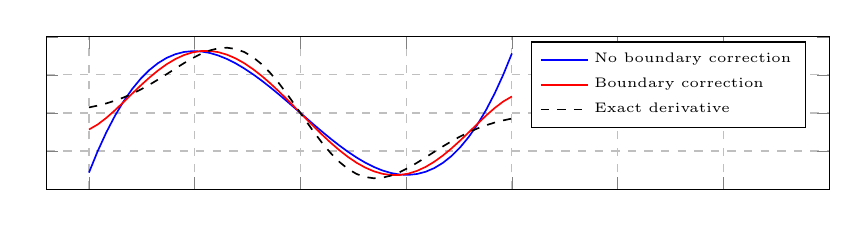
\begin{tikzpicture}
\begin{axis}[
    width=.95\textwidth,
    height=10em,
%    xlabel={$x$ coordinate},
%    ylabel={$L^2$ errors}, 
    xmin=-1.2, xmax=2.5,
    ymin=-2, ymax=2,
    legend pos=north east, legend cell align=left, legend style={font=\tiny},	
    xmajorgrids=true, ymajorgrids=true, grid style=dashed,
%    legend entries={GSBP, Decoupled, Exact}    
yticklabels={,,},
xticklabels={,,},
legend entries={No boundary correction, Boundary correction, Exact derivative}
]
\pgfplotsset{
%cycle list={{blue, only marks, mark=*}, {blue}, {red, only marks,mark=square*},{red},{black,dashed}}
cycle list={{blue},{red},{black,dashed}}
%cycle list={{blue},{black,dashed}}
}
%\addlegendimage{blue, mark=*}
%\addlegendimage{red, mark=square*}
%\addlegendimage{black, dashed}

%\addplot+[semithick, mark options={solid, fill=markercolor}]
%coordinates{(-0.93247,-0.677965)(-0.661209,1.35632)(-0.238619,1.07263)(0.238619,-1.07263)(0.661209,-1.35632)(0.93247,0.677965)};

\addplot+[semithick, mark options={solid, fill=markercolor}]
coordinates{(-1,-1.56577)(-0.959184,-1.00891)(-0.918367,-0.51366)(-0.877551,-0.0774098)(-0.836735,0.302464)(-0.795918,0.628585)(-0.755102,0.903575)(-0.714286,1.13006)(-0.673469,1.31065)(-0.632653,1.44798)(-0.591837,1.54466)(-0.55102,1.60333)(-0.510204,1.62659)(-0.469388,1.61708)(-0.428571,1.57742)(-0.387755,1.51022)(-0.346939,1.41812)(-0.306122,1.30372)(-0.265306,1.16966)(-0.22449,1.01856)(-0.183673,0.85303)(-0.142857,0.675704)(-0.102041,0.489201)(-0.0612245,0.296143)(-0.0204082,0.0991513)(0.0204082,-0.0991513)(0.0612245,-0.296143)(0.102041,-0.489201)(0.142857,-0.675704)(0.183673,-0.85303)(0.22449,-1.01856)(0.265306,-1.16966)(0.306122,-1.30372)(0.346939,-1.41812)(0.387755,-1.51022)(0.428571,-1.57742)(0.469388,-1.61708)(0.510204,-1.62659)(0.55102,-1.60333)(0.591837,-1.54466)(0.632653,-1.44798)(0.673469,-1.31065)(0.714286,-1.13006)(0.755102,-0.903575)(0.795918,-0.628585)(0.836735,-0.302464)(0.877551,0.0774098)(0.918367,0.51366)(0.959184,1.00891)(1,1.56577)};

%\addplot+[semithick, mark options={solid, fill=markercolor}]
%coordinates{(-0.93247,-0.194074)(-0.661209,1.16978)(-0.238619,1.20913)(0.238619,-1.20913)(0.661209,-1.16978)(0.93247,0.194074)};

\addplot+[semithick, mark options={solid, fill=markercolor}]
coordinates{(-1,-0.434491)(-0.959184,-0.303266)(-0.918367,-0.130624)(-0.877551,0.0698403)(-0.836735,0.286078)(-0.795918,0.507515)(-0.755102,0.724981)(-0.714286,0.930644)(-0.673469,1.11794)(-0.632653,1.28151)(-0.591837,1.41712)(-0.55102,1.5216)(-0.510204,1.59278)(-0.469388,1.62942)(-0.428571,1.63111)(-0.387755,1.59825)(-0.346939,1.53198)(-0.306122,1.43404)(-0.265306,1.30681)(-0.22449,1.15314)(-0.183673,0.976347)(-0.142857,0.78012)(-0.102041,0.568459)(-0.0612245,0.345602)(-0.0204082,0.115959)(0.0204082,-0.115959)(0.0612245,-0.345602)(0.102041,-0.568459)(0.142857,-0.78012)(0.183673,-0.976347)(0.22449,-1.15314)(0.265306,-1.30681)(0.306122,-1.43404)(0.346939,-1.53198)(0.387755,-1.59825)(0.428571,-1.63111)(0.469388,-1.62942)(0.510204,-1.59278)(0.55102,-1.5216)(0.591837,-1.41712)(0.632653,-1.28151)(0.673469,-1.11794)(0.714286,-0.930644)(0.755102,-0.724981)(0.795918,-0.507515)(0.836735,-0.286078)(0.877551,-0.0698403)(0.918367,0.130624)(0.959184,0.303266)(1,0.434491)};

\addplot+[semithick, mark options={solid, fill=markercolor}]
coordinates{(-1,0.146525)(-0.959184,0.193522)(-0.918367,0.251752)(-0.877551,0.322529)(-0.836735,0.406852)(-0.795918,0.50522)(-0.755102,0.617438)(-0.714286,0.742415)(-0.673469,0.877994)(-0.632653,1.02082)(-0.591837,1.1663)(-0.55102,1.30861)(-0.510204,1.44089)(-0.469388,1.55553)(-0.428571,1.64452)(-0.387755,1.70003)(-0.346939,1.71492)(-0.306122,1.68342)(-0.265306,1.60163)(-0.22449,1.46805)(-0.183673,1.2839)(-0.142857,1.05327)(-0.102041,0.783025)(-0.0612245,0.482507)(-0.0204082,0.162994)(0.0204082,-0.162994)(0.0612245,-0.482507)(0.102041,-0.783025)(0.142857,-1.05327)(0.183673,-1.2839)(0.22449,-1.46805)(0.265306,-1.60163)(0.306122,-1.68342)(0.346939,-1.71492)(0.387755,-1.70003)(0.428571,-1.64452)(0.469388,-1.55553)(0.510204,-1.44089)(0.55102,-1.30861)(0.591837,-1.1663)(0.632653,-1.02082)(0.673469,-0.877994)(0.714286,-0.742415)(0.755102,-0.617438)(0.795918,-0.50522)(0.836735,-0.406852)(0.877551,-0.322529)(0.918367,-0.251752)(0.959184,-0.193522)(1,-0.146525)};
\end{axis}
\end{tikzpicture}
\end{figure}
\vspace{-1em}
\begin{itemize}
%\item Combine $\bm{D}^i_N$ with $L^2$ projection to approximate derivatives.
%\vspace{.25em}
\item $\bm{D}^i_N$ produces a high order approximation of $f\pd{g}{x}$ at $\bm{x} = [\bm{x}^q, \bm{x}^f]$.
\[
f\pd{g}{x} \approx \LRs{\begin{array}{cc}
\bm{P}_q & \bm{L}_f\end{array}} {\rm diag}\LRp{\bm{f}}\bm{D}_N \bm{g}, \qquad \bm{f}_i, \bm{g}_i = f(\bm{x}_i), g(\bm{x}_i).
\]
\item Reduces to traditional SBP operator under appropriate quadrature. 
\vspace{.25em}
\item Equivalent to a \note{skew-symmetric} variational problem for $u(\bm{x}) \approx f\pd{g}{x}$.
\[
\int_{D^k}u(\bm{x})v(\bm{x})  = \int_{D^k}{f\pd{P_Ng}{x}v} + \int_{\partial D^k}{(g-P_Ng)\frac{\LRp{fv + P_N(fv)}}{2}}.
\]
\end{itemize}
}


\section{Entropy stable formulations and flux differencing}
\frame[noframenumbering]{
\frametitle{Talk outline}
\tableofcontents[currentsection]
}

\frame{
\frametitle{Burgers' equation: decoupled SBP and energy stability}
\setcounter{subfigure}{0}
\begin{itemize}
\item Revisit split form of Burgers' equation:
\[
\pd{u}{t} + \frac{1}{3}\LRp{\pd{u^2}{x} + {u\pd{u}{x}}} = 0
\]
\item ``Modal'' DG method: let $u_h(x) = \sum_j \hat{\bm{u}}_j \phi(x)$.  Find $\hat{\bm{u}}$ such that 
\begin{align*}
&\bm{u} = \LRs{\begin{array}{c}
\bm{V}_q\\
\bm{V}_f
\end{array}} \hat{\bm{u}}, \qquad \bm{f}^* = \bm{f}^*(u^+,u) = \text{numerical flux} \\
%
&\bm{M}\td{\hat{\bm{u}}}{t} + \frac{1}{3}
\LRs{\begin{array}{c}
\bm{V}_q \\ \bm{V}_f\end{array}}^T
\LRp{\bm{Q}_N \LRp{\bm{u}^2} + {\rm diag}\LRp{\bm{u}} \bm{Q}_N \bm{u}} + \bm{V}_f^T\bm{B} \bm{f}^* = 0.
%
%&\td{\hat{\bm{u}}}{t} + \frac{1}{3}
%\LRs{\begin{array}{cc}
%\bm{P}_q & \bm{L}_f\end{array}}
%\LRp{\bm{D}_N \LRp{\bm{u}^2} + {\rm diag}\LRp{\bm{u}} \bm{D}_N \bm{u}} + \bm{L}_f \bm{B} (\bm{f}^*) = 0.
\end{align*}
\item Formulation is energy stable for \note{arbitrary volume quadratures}
\[
\td{}{t}\hat{\bm{u}}^T\bm{M}\hat{\bm{u}}  = \pd{}{t}\nor{u_h}^2 \leq 0
\]
%: multiply by $\hat{\bm{u}}^T\bm{M}$, use SBP, sum over $D^k$
%\[
%\sum_k \frac{1}{2}\td{}{t}\hat{\bm{u}}^T\bm{M}\hat{\bm{u}} = \sum_k \frac{1}{2} \pd{}{t}\nor{u}^2_{L^2\LRp{D^k}} \leq 0.
%\]
\end{itemize}
}

\frame{
\frametitle{Burgers' equation: energy stable shock solution}
\setcounter{subfigure}{0}

\begin{figure}
\begin{overlayarea}{\textwidth}{.5\textheight}
%\begin{overprint}
\centering
\foreach \id in {1,2,3,4,5,6,7,8}{%
\only<\id>{
\subfloat[$\tau = 0$]{\includegraphics[width=.425\textwidth]{figs/burgersStableEC_\id.png}}\hspace{2em}%
\subfloat[$\tau = 1$]{\includegraphics[width=.425\textwidth]{figs/burgersStableLF_\id.png}}
}% \only
}% for
\only<9>{
\captionsetup[subfloat]{width=.45\textwidth, justification=centering}
\subfloat[Energy conservative ($\tau = 0$)]{\includegraphics[width=.45\textwidth]{figs/burgersSplitEnergyEC.png}}\hspace{1em}%
\subfloat[Energy stable ($\tau = 1$)]{\includegraphics[width=.45\textwidth]{figs/burgersSplitEnergyLF.png}}
}
%\end{overprint}
\end{overlayarea}
\end{figure}
}


% =================================================

%\frame{
%\frametitle{Challenges for summation-by-parts formulations (SBP)}
%\setcounter{subfigure}{0}
%\begin{itemize} 
%\item Construction using \note{nodal collocation} at quadrature points.  
%\item Need at least $2N-1$ accurate volume and surface quadrature! 
%\item Difficult to generalize beyond polynomial DG (splines, pyramids, etc).
%\end{itemize}
%\vspace{-.5em}
%\begin{figure}
%\centering
%\begingroup
%\captionsetup[subfloat]{width=.3\textwidth}
%\subfloat[Tensor product SBP nodes (GLL quadrature)]{\includegraphics[width=.32\textwidth]{figs/SEM_stencil_1.pdf}}
%\hspace{1em}
%\subfloat[Interpolation nodes ($N=4$, 15 pts)]{\includegraphics[width=.25\textwidth]{figs/triNodesN4.png}}
%\hspace{.5em}
%\subfloat[Diag-norm SBP nodes ($N=4$, 22 pts)]{\includegraphics[width=.25\textwidth]{figs/chenShuNodes.png}}
%\endgroup
%%\caption{Dif.}
%\end{figure}
%
%\let\thefootnote\relax\footnotetext{\tiny Chen and Shu (2017). \textit{ES high order DG methods with suitable quadrature rules for hyperbolic conservation laws.}}
%\let\thefootnote\relax\footnotetext{\tiny Chan and Evans (2017). \textit{Multi-patch DG spline finite element methods for time-domain wave propagation}.}
%}


% =================================================

%\section{Flux differencing and discrete entropy conservation}
%\frame[noframenumbering]{
%\frametitle{Talk outline}
%\tableofcontents[currentsection]
%}

\frame{
\frametitle{Entropy conservative finite volume fluxes}

\begin{itemize}
\item<1-> Tadmor's entropy conservative numerical flux: 
\begin{align*}
\bm{f}_S(\bm{u},\bm{u}) &= \bm{f}(\bm{u}), \qquad \text{(consistency)} \\
\bm{f}_S(\bm{u},\bm{v}) &= \bm{f}_S(\bm{v},\bm{u}),\qquad \text{(symmetry)} \\
\LRp{\bm{v}_L - \bm{v}_R}^T \bm{f}\LRp{\bm{u}_L,\bm{u}_R} &= \psi_L - \psi_R, \qquad \text{(conservation)}.
\end{align*}
\item<2-> Example: entropy conservative flux for Burgers' equation 
\[
f_S(u_L,u_R) = \frac{1}{6}\LRp{u_L^2 + u_Lu_R + u_R^2}.
\]
\item<3-> Flux differencing: use finite volume fluxes to evaluate derivatives.% in DG methods.
%\item<3-> Flux differencing for Burgers' equation: let $u_L = u(x), u_R = u(y)$
%\begin{align*}
%&f_S(u(x),u(y)) = \frac{1}{6}\LRp{u(x)^2 + u(x)u(y) + u(y)^2},\\
%&\pd{{f}({u})}{x} \Longrightarrow \note{\LRu{2\pd{f_S\LRp{u(x),u(y)}}{x}}_{y=x}} = \frac{1}{3}\pd{u^2}{x} + \frac{1}{3}u\pd{u}{x} + \frac{1}{3}u^2\cancel{\pd{1}{x}}.
%\end{align*}
\end{itemize}

\let\thefootnote\relax\footnotetext{\tiny Tadmor, Eitan (1987). \textit{The numerical viscosity of entropy stable schemes for systems of conservation laws. I.}}
}

\frame{
\frametitle{Flux differencing: recovering split formulations}
\begin{itemize}
\item<1-> Entropy conservative flux for Burgers' equation 
\[
f_S(u_L,u_R) = \frac{1}{6}\LRp{u_L^2 + u_Lu_R + u_R^2}.
\]
\item<1-> Flux differencing: let $u_L = u(x), u_R = u(y)$
\begin{align*}
\pd{{f}({u})}{x} &\Longrightarrow \note{\LRu{2\pd{f_S\LRp{u(x),u(y)}}{x}}_{y=x}}
\end{align*}
\item<2-> Recovering the Burgers' split formulation
\begin{align*}
f_S(u(x),u(y)) &= \frac{1}{6}\LRp{u(x)^2 + u(x)u(y) + u(y)^2}\\
\LRu{2\pd{f_S\LRp{u(x),u(y)}}{x}}_{y=x} &= \frac{1}{3}\pd{u^2}{x} + \frac{1}{3}u\pd{u}{x} + \frac{1}{3}u^2\cancel{\pd{1}{x}}.
\end{align*}
\end{itemize}
}

\frame{
\frametitle{Flux differencing: beyond split formulations}
\begin{itemize}
\item Fluxes do not necessarily correspond to split formulations!  
\vspace{.5em}
\item Example: entropy conservative flux for 1D compressible Euler
\begin{align*}
f^1_S(\bm{u}_L,\bm{u}_R) &= \avg{\rho}^{\log} \avg{u}\\
f^2_S(\bm{u}_L,\bm{u}_R) &= \frac{\avg{\rho}}{2\avg{\beta}} + \avg{u}f^1_S\\
f^3_S(\bm{u}_L,\bm{u}_R) &= f^1_S\LRp{\frac{1}{2(\gamma-1)\avg{\beta}^{\log}} - \frac{1}{2}\avg{u^2}} + \avg{u}f^2_S,
\end{align*}
%\vspace{.5em}
\item Rational functions: logarithmic mean and ``inverse temperature'' $\beta$
\[
\avg{u}^{\log} = \frac{u_L - u_R}{\log{u_L}- \log{u_R}}, \qquad \beta = \frac{\rho}{2p}.
\]
\end{itemize}

\let\thefootnote\relax\footnotetext{\tiny Chandreshekar (2013),  \emph{Kinetic energy preserving and entropy stable FV schemes for comp.\ Euler and NS equations.}}
}

\frame{
\frametitle{Flux differencing: implementational details}
\begin{itemize}
%\item Flux differencing necessary for general nonlinear conservation laws (compressible Euler), not for split forms (Burgers, shallow water).  
\item Define ${\bm{F}_S}$ by evaluating $\bm{f}_S$ at all combinations of quadrature points
\[
\LRp{\bm{F}_S}_{ij} = \bm{f}_S\LRp{u(\bm{x}_i),u(\bm{x}_j)}, \qquad \bm{x} = \LRs{\bm{x}^q,\bm{x}^f}^T.
\]
\item Replace $\pd{}{x}$ with the decoupled SBP operator $\bm{D}_N$ + polynomial $L^2$ projection and lifting matrices.
\[
\LRu{2\pd{f_S\LRp{u(x),u(y)}}{x}}_{y=x} \Longrightarrow \LRs{\begin{array}{cc}
\bm{P}_q & \bm{L}_f\end{array}}
{\rm diag}{\LRp{2\bm{D}_N \bm{F}_S}}.
\]
\vspace{.001em}
\item Simpler \note{Hadamard product} reformulation: evaluate $\bm{F}_S$ on-the-fly 
\[
{\rm diag}{\LRp{2\bm{D}_N \bm{F}_S}} = \LRp{2\bm{D}_N \circ \bm{F}_S}\bm{1}.
\]
\end{itemize}

%\let\thefootnote\relax\footnotetext{\tiny Chandrashekar (2013). \textit{Kinetic energy preserving and entropy stable FV schemes for compressible Euler and NS equations.}}
}

%\frame{
%\frametitle{Entropy stable high order DG: implementation}
%
%\begin{itemize}
%\item Right hand side evaluation for explicit time-stepping:
%\begin{enumerate}
%\item Compute $L^2$ projection of entropy variables $P_N\LRp{\bm{v}(\bm{u})}$.
%\item Eval.\ conservative variables $\bm{u}(P_N\LRp{\bm{v}(\bm{u})})$ at quadrature points.
%\item Compute $\bm{RHS}(\bm{u}) = {\rm diag}\LRp{2\bm{D}^x_h \bm{f}_S\LRp{\bm{u}_x,\bm{u}_y}}$
%%\item Compute $\bm{RHS}(\bm{u}) = 2\LRp{\bm{D}_h \circ \bm{F}_S}\bm{1}$
%\end{enumerate}
%\vspace{1em}
%\item Efficient \note{Hadamard product} reformulation (low-memory evaluation)
%\begin{align*}
%\LRs{\begin{array}{c}
%\bm{P}_q\\
%\bm{L}_f\end{array}}
%{\rm diag}{\LRp{2\bm{D}_N \bm{F}_S}}.
%\] = 
%\end{align*}
%%\vspace{1em}
%%\item Simplifications for diag-norm SBP (nodal collocation): avoid computing projections, combine volume + surface operations.
%\end{itemize}
%}
%% =================================================

\frame{
\frametitle{Flux differencing circumvents the chain rule} 

\vspace{-.5em}
\begin{itemize}
\item Test with entropy variables $\tilde{\bm{v}}$, integrate, and use SBP property:
\[
\tilde{\bm{v}}^T\LRp{2\bm{Q}_N \circ \bm{F}_S}\bm{1} = \tilde{\bm{v}}^T\LRp{\LRp{
%\LRs{\begin{array}{cc}
%0 &\\
%& \bm{W}_f\bm{n}
%\end{array}}
\bm{B}_N
 + \bm{Q}_N - \bm{Q}_N^T} \circ \bm{F}_S}\bm{1}.
\]
\item Only boundary terms appear in final estimate; volume terms become boundary terms using properties of $\LRp{\bm{F}_S}_{ij} = \bm{f}_S\LRp{\tilde{\bm{u}}_i,\tilde{\bm{u}}_j}$
\begin{overlayarea}{\textwidth}{.3\textheight}
\begin{align*}
\tilde{\bm{v}}^T\LRp{\LRp{\bm{Q}_N - \bm{Q}_N^T} \circ \bm{F}_S}\bm{1} 
&= \tilde{\bm{v}}^T\LRp{\bm{Q}_N \circ \bm{F}_S}\bm{1} - \bm{1}^T\LRp{\bm{Q}_N \circ \bm{F}_S}\tilde{\bm{v}}  \\
\only<1>{&= \sum_{i,j} \LRp{\bm{Q}_N}_{ij} \textcolor{red}{\LRp{\tilde{\bm{v}}_i - \tilde{\bm{v}}_j}^T\bm{f}_S\LRp{\tilde{\bm{u}}_i,\tilde{\bm{u}}_j}}.}
\only<2>{&= \sum_{i,j} \LRp{\bm{Q}_N}_{ij} \textcolor{red}{\LRp{\psi(\tilde{\bm{u}}_i)-\psi(\tilde{\bm{u}}_j)}.}}
\only<3>{&= \textcolor{red}{\bm{1}^T\bm{Q}_N \bm{\psi} - \bm{\psi}^T\bm{Q}_N\bm{1} = \bm{1}^T\bm{Q}_N \bm{\psi} }}
\only<4->{&= \textcolor{red}{\bm{1}^T\LRp{\bm{B}_N-\bm{Q}_N^T} \bm{\psi} = \bm{1}^T\bm{B}_N\bm{\psi}.
}}
\end{align*}
\end{overlayarea}
%\vspace{.25em}
%\item Let $\bm{v}_q$ be entropy variables at quadrature points.  Multiply by $\LRp{\bm{P}_q\bm{v}}^T\bm{M}$
%\[
%\bm{v}_q^T \bm{P}_q^T \bm{M} \td{\hat{\bm{u}}}{t} = \bm{v}_q^T \bm{W} \bm{V}_q \bm{M}^{-1}\bm{M} \td{\hat{\bm{u}}}{t} = \bm{v}_q^T \bm{W}  \td{\LRp{\bm{V}_q\hat{\bm{u}}}}{t} = .  
%\]
\item<5-> Proof uses \note{$\LRp{\tilde{\bm{v}}_i - \tilde{\bm{v}}_j}^T\bm{f}_S\LRp{\tilde{\bm{u}}_i,\tilde{\bm{u}}_j} = \psi(\tilde{\bm{u}}_i)-\psi(\tilde{\bm{u}}_j)$}:   
%$\tilde{\bm{v}} = \bm{v}(\tilde{\bm{u}})$; the 
requires entropy variables $\tilde{\bm{v}}$ to be a function of conservative variables $\tilde{\bm{u}}$. %; modify conservative variables $\tilde{\bm{u}}$ to ensure test function $\bm{v}(\tilde{\bm{u}}) = P_N\bm{v}(\bm{u}) \in P^N$.
%\item<4-> Proof requires $\bm{v} = \bm{v}(\bm{u})$ \textcolor{red}{pointwise}; modify conservative variables $\tilde{\bm{u}}$ to ensure test function $\bm{v}(\tilde{\bm{u}}) = P_N\bm{v}(\bm{u}) \in P^N$.
\end{itemize} 
}

\frame{
\frametitle{Modifying the conservative variables} 

\begin{itemize}
\item Conservative variables $\bm{u}_h$ and test functions are polynomial, but the entropy variables $\bm{v}(\bm{u}_h)\not\in P^N$!
\vspace{1em}
\item Evaluate flux $\bm{f}_S$ using \note{modified} conservative variables $\tilde{\bm{u}}$
\[
\tilde{\bm{u}} = \bm{u}\LRp{P_N\bm{v}(\bm{u}_h)}.
\]
%\vspace{1em}
\item \note{If $\bm{v}(\bm{u})$ is an invertible mapping}, this choice of $\tilde{\bm{u}}$ ensures that 
\[
\tilde{\bm{v}} = \bm{v}(\tilde{\bm{u}}) = P_N\bm{v}(\bm{u}_h) \in P^N.
\]
%\vspace{1em}
\item Local conservation w.r.t.\ a generalized Lax-Wendroff theorem.
\end{itemize}
\let\thefootnote\relax\footnotetext{\tiny Shi and Shu (2017). \emph{On local conservation of numerical methods for conservation laws}.}
}

\frame{
\frametitle{Illustration of main steps of ESDG}
\begin{columns}
\hspace{-1em}
\begin{column}{.48\textwidth}
\vspace{-1em}
\begin{figure}
%\centering
\begin{overlayarea}{.75\textwidth}{.425\textheight}
\only<1>{\includegraphics[height=.42\textheight]{figs/gsbp_tri1.png}}
\only<2>{\includegraphics[height=.42\textheight]{figs/gsbp_tri2.png}}
\only<3>{\includegraphics[height=.42\textheight]{figs/gsbp_tri3.png}}
\only<4>{\includegraphics[height=.42\textheight]{figs/gsbp_tri4.png}}
\end{overlayarea}
\end{figure}
\end{column}
\hspace{3em}
\begin{column}{.5\textwidth}
\[
\only<1>{
\LRp{\underbrace{\begin{bmatrix}
\bm{A} & \bm{B}\\
-\bm{B}^T & \bm{C}
\end{bmatrix}}_{\bm{Q}_N^i} \circ
\underbrace{\begin{bmatrix}
\bm{F}^{vv}_S & \bm{F}^{vf}_S\\
\bm{F}^{fv}_S & \bm{F}^{ff}_S
\end{bmatrix}}_{\bm{F}_S} } \bm{1}
}
\only<2>{
\LRp{\underbrace{\begin{bmatrix}
\note{\bm{A}} & \bm{B}\\
-\bm{B}^T & \bm{C}
\end{bmatrix}}_{\bm{Q}_N^i} \circ
\underbrace{\begin{bmatrix}
\note{\bm{F}^{vv}_S} & \bm{F}^{vf}_S\\
\bm{F}^{fv}_S & \bm{F}^{ff}_S
\end{bmatrix}}_{\bm{F}_S} } \bm{1}
}
\only<3>{
\LRp{\underbrace{\begin{bmatrix}
\bm{A} & \bm{B}\\
-\bm{B}^T & \note{\bm{C}}
\end{bmatrix}}_{\bm{Q}_N^i} \circ
\underbrace{\begin{bmatrix}
\bm{F}^{vv}_S & \bm{F}^{vf}_S\\
\bm{F}^{fv}_S & \note{\bm{F}^{ff}_S}
\end{bmatrix}}_{\bm{F}_S} } \bm{1}
}
\only<4>{
\LRp{\underbrace{\begin{bmatrix}
\bm{A} & \note{\bm{B}}\\
\note{-\bm{B}^T} & \bm{C}
\end{bmatrix}}_{\bm{Q}_N^i} \circ
\underbrace{\begin{bmatrix}
\bm{F}^{vv}_S & \note{\bm{F}^{vf}_S}\\
\note{\bm{F}^{fv}_S} & \bm{F}^{ff}_S
\end{bmatrix}}_{\bm{F}_S} } \bm{1}
}
\]
\end{column}
\end{columns}
\vspace{.5em}
\begin{itemize}
\item<1-> Interpolate \note{projected entropy variables $P_N \bm{v}(\bm{u})$} to all nodes.  
%\vspace{.5em}
\item<2-> Compute interactions $\bm{f}_S(\bm{u}_L, \bm{u}_R)$ between \note{volume quadrature nodes}.
%\vspace{.5em}
\item<3-> Compute interactions between \note{surface nodes} of neighboring elements
\item<4-> Compute interactions between \note{volume and surface} nodes.
\end{itemize} 
}

\frame{
\frametitle{A general entropy conservative DG formulation}
\vspace{-1em}
%\begin{overlayarea}{\textwidth}{.9\textheight}d
\begin{theorem}[Chan 2018]
Let $\bm{u}_h(\bm{x}) = \sum_j \hat{\bm{u}}_j \phi_j(\bm{x})$ and $\tilde{\bm{u}} = \bm{u}\LRp{P_N\bm{v}}$.  Let $\hat{\bm{u}}$ locally solve 
\[
%\td{\hat{\bm{u}}}{t} + \sum_{i=1}^d\LRs{\begin{array}{cc}
%\bm{P}_q & \bm{L}_f\end{array}} \LRp{2\bm{D}^i_N \circ \bm{F}^i_S}\bm{1} + \bm{L}_f \LRp{\bm{f}^i_S(\tilde{\bm{u}}^+,\tilde{\bm{u}}) - \bm{f}^i(\tilde{\bm{u}})}\bm{n}_i = 0.
\bm{M}\td{\hat{\bm{u}}}{t} + \sum_{i=1}^d\LRs{\begin{array}{c}
\bm{V}_q \\ \bm{V}_f\end{array}}^T \LRp{2\bm{Q}^i_N \circ \bm{F}^i_S}\bm{1} + \bm{V}_f^T\bm{B}_i \LRp{\bm{f}^i_S(\tilde{\bm{u}}^+,\tilde{\bm{u}}) - \bm{f}^i(\tilde{\bm{u}})} = 0.
\]
Assuming continuity in time, $\bm{u}_h(\bm{x})$ satisfies the quadrature form of
\[
\int_{\Omega} \pd{S(\bm{u}_h)}{t} + \sum_{i=1}^d\int_{\partial \Omega} \LRp{(P_N\bm{v})^T\bm{f}^i(\tilde{\bm{u}}) - \psi_i(\tilde{\bm{u}})} \bm{n}_i = 0.
\]
%\[
%\int_{\Omega} \pd{S}{t} + \int_{\partial \Omega} \bm{v}^T\bm{f}(\bm{u}) - \psi(\bm{u}) = 0.
%\]
\end{theorem} 
%\only<5>{
%\vspace{-.25em}
\begin{itemize}
%\item Note: $\bm{u}\in P^N$, but $\bm{v}(\bm{u}) \not\in P^N$! 
% Entropy conservation uses $L^2$-\note{projected} entropy variables $P_N \bm{v}$ and redefined $\tilde{\bm{u}} = \bm{u}\LRp{P_N\bm{v}}$!
\item Can modify interface flux (e.g.\ Lax-Friedrichs or matrix dissipation) to change the entropy equality to an entropy \note{inequality}. 
\end{itemize}

%\let\thefootnote\relax\footnotetext{\tiny Chan (2018). \textit{On discretely entropy conservative and entropy stable discontinuous Galerkin methods.}}
\let\thefootnote\relax\footnotetext{\tiny Winters, Derigs, Gassner, and Walch (2017). \textit{A uniquely defined entropy stable matrix dissipation operator for high Mach number ideal MHD and compressible Euler simulations.}}
}


%% =================================================

\section{Numerical experiments}

%\subsection{1D experiments }

\frame[noframenumbering]{
\frametitle{Talk outline}
\only<1>{
\tableofcontents[currentsection]
}
\only<2>{
\tableofcontents[currentsection,currentsubsection]
}
}

%\frame{
%\frametitle{1D compressible Euler equations}
%
%\begin{itemize}
%\item Inexact Gauss-Legendre-Lobatto (GLL) vs Gauss (GQ) quadratures. 
%\item Entropy conservative (EC) and dissipative Lax-Friedrichs (LF) fluxes.  
%\item No additional stabilization, filtering, or limiting.
%%\item $L^2$ rates: odd/even decoupling for EC, $O(h^{N+1})$ for LF.
%\end{itemize} 
%\vspace{-1em}
%\begin{figure}
%\centering
%\subfloat[Entropy conservative flux]{
%\begin{tikzpicture}
%\begin{loglogaxis}[
%    width=.49\textwidth,
%    xlabel={Mesh size $h$},
%%    ylabel={$L^2$ errors}, 
%    xmin=.0075, xmax=.75,
%    ymin=1e-11, ymax=2,
%    legend pos=south east, legend cell align=left, legend style={font=\tiny},	
%    xmajorgrids=true, ymajorgrids=true, grid style=dashed,
%    legend entries={GLL,GQ-$(N+2)$}    
%]
%\pgfplotsset{
%cycle list={{blue, dashed, mark=*}, {red, mark=square*}}
%}
%%\addlegendimage{no markers,blue}
%%\addlegendimage{no markers,red}
%
%\addplot+[semithick, mark options={solid, fill=markercolor}]
%% N = 1, tau = 0.000000 =======================
%coordinates{(0.5,1)(0.25,0.485059)(0.125,0.203599)(0.0625,0.0947163)(0.03125,0.0463705)};
%\addplot+[semithick, mark options={solid, fill=markercolor}]
%%N = 1, tau = 0.000000 =======================
%coordinates{(0.5,0.402314)(0.25,0.167917)(0.125,0.106574)(0.0625,0.058359)(0.03125,0.0298728)}
%[yshift=1pt] node[left, pos=1.025, color=black] {$N = 1$};
%
%
%\addplot+[semithick, mark options={solid, fill=markercolor}]
%% N = 2, tau = 0.000000 =======================
%coordinates{(0.5,0.746606)(0.25,0.156701)(0.125,0.0137392)(0.0625,0.000701926)(0.03125,8.64531e-05)};
%\addplot+[semithick, mark options={solid, fill=markercolor}]
%%N = 2, tau = 0.000000 =======================
%coordinates{(0.5,0.993771)(0.25,0.0219437)(0.125,0.00180028)(0.0625,0.000194939)(0.03125,2.4045e-05)}
%[yshift=4pt] node[left, pos=1.025, color=black] {$N = 2$};
%
%
%\addplot+[semithick, mark options={solid, fill=markercolor}]
%% N = 3, tau = 0.000000 =======================
%coordinates{(0.5,0.103299)(0.25,0.00829887)(0.125,0.00073573)(0.0625,9.05975e-05)(0.03125,1.13596e-05)};
%\addplot+[semithick, mark options={solid, fill=markercolor}]
%%N = 3, tau = 0.000000 =======================
%coordinates{(0.5,0.0154054)(0.25,0.00167426)(0.125,0.000260859)(0.0625,3.76182e-05)(0.03125,3.86238e-06)}
%[yshift=1pt] node[left, pos=1.025, color=black] {$N = 3$};
%
%\addplot+[semithick, mark options={solid, fill=markercolor}]
%% N = 4, tau = 0.000000 =======================
%coordinates{(0.5,0.0385542)(0.25,0.00133048)(0.125,0.000176663)(0.0625,1.64135e-06)(0.03125,2.66024e-08)};
%\addplot+[semithick, mark options={solid, fill=markercolor}]
%%N = 4, tau = 0.000000 =======================
%coordinates{(0.5,0.0367592)(0.25,0.000202817)(0.125,3.57758e-06)(0.0625,9.58294e-08)(0.03125,2.94985e-09)}[yshift=6pt] node[left, pos=1.025, color=black] {$N = 4$};
%
%\addplot+[semithick, mark options={solid, fill=markercolor}]
%% N = 5, tau = 0.000000 =======================
%coordinates{(0.5,0.00436131)(0.25,0.00039846)(0.125,2.1282e-06)(0.0625,4.49046e-08)(0.03125,9.99912e-10)};
%\addplot+[semithick, mark options={solid, fill=markercolor}]
%%N = 5, tau = 0.000000 =======================
%coordinates{(0.5,0.000390565)(0.25,1.31188e-05)(0.125,3.6544e-07)(0.0625,4.95271e-09)(0.03125,2.42763e-10)}
%[yshift=3pt] node[left, pos=1.025, color=black] {$N = 5$};
%
%%\legend{$N=1$,$N=2$,$N=3$,$N=4$,$N=5$}
%\end{loglogaxis}
%\end{tikzpicture}
%}
%\subfloat[With Lax-Friedrichs penalization]{
%\begin{tikzpicture}
%\begin{loglogaxis}[
%    width=.49\textwidth,
%    xlabel={Mesh size $h$},  %ylabel={$L^2$ errors}, 
%    xmin=.0075, xmax=.75,
%    ymin=1e-11, ymax=2,
%    legend pos=south east, legend cell align=left, legend style={font=\tiny},	
%    xmajorgrids=true, ymajorgrids=true, grid style=dashed,
%    legend entries={GLL,GQ-$(N+2)$}
%] 
%\pgfplotsset{
%cycle list={{blue, dashed, mark=*}, {red, mark=square*}}
%}
%%\pgfplotsset{cycle list={{blue, dashed, mark=*}, {red, mark=square*}}}
%
%\addplot+[semithick, mark options={solid, fill=markercolor}]
%% N = 1, tau = 0.500000 =======================
%coordinates{(0.5,1)(0.25,0.4932)(0.125,0.183839)(0.0625,0.0562398)(0.03125,0.0151873)};
%\addplot+[semithick, mark options={solid, fill=markercolor}]
%%N = 1, tau = 0.500000 =======================
%coordinates{(0.5,0.547558)(0.25,0.148981)(0.125,0.0384647)(0.0625,0.00974763)(0.03125,0.00244539)}
%[yshift=5pt] node[left, pos=1.025, color=black] {$N = 1$};
%
%\addplot+[semithick, mark options={solid, fill=markercolor}]	
%% N = 2, tau = 0.500000 =======================
%coordinates{(0.5,0.336817)(0.25,0.04941)(0.125,0.00605428)(0.0625,0.000748842)(0.03125,9.25456e-05)};
%\addplot+[semithick, mark options={solid, fill=markercolor}]
%%N = 2, tau = 0.500000 =======================
%coordinates{(0.5,0.165807)(0.25,0.0190013)(0.125,0.00227903)(0.0625,0.00028425)(0.03125,3.54865e-05)}
%[yshift=3pt] node[left, pos=1.025, color=black] {$N = 2$};
%
%
%% N = 3, tau = 0.500000 =======================
%\addplot+[semithick, mark options={solid, fill=markercolor}]
%coordinates{(0.5,0.0463242)(0.25,0.00408748)(0.125,0.000346831)(0.0625,1.99064e-05)(0.03125,1.22357e-06)};
%\addplot+[semithick, mark options={solid, fill=markercolor}]
%%N = 3, tau = 0.500000 =======================
%coordinates{(0.5,0.0174194)(0.25,0.00182234)(0.125,0.000116147)(0.0625,7.39839e-06)(0.03125,4.6305e-07)}
%[yshift=3pt] node[left, pos=1.025, color=black] {$N = 3$};
%
%\addplot+[semithick, mark options={solid, fill=markercolor}]
%% N = 4, tau = 0.500000 =======================
%coordinates{(0.5,0.0100716)(0.25,0.000625923)(0.125,1.89866e-05)(0.0625,7.03865e-07)(0.03125,2.10265e-08)};
%\addplot+[semithick, mark options={solid, fill=markercolor}]
%%N = 4, tau = 0.500000 =======================
%coordinates{(0.5,0.00556743)(0.25,0.000144595)(0.125,4.33972e-06)(0.0625,1.37151e-07)(0.03125,4.16335e-09)}
%[yshift=4pt] node[left, pos=1.025, color=black] {$N = 4$};
%
%
%\addplot+[semithick, mark options={solid, fill=markercolor}]
%% N = 5, tau = 0.500000 =======================
%coordinates{(0.5,0.00356628)(0.25,8.73125e-05)(0.125,2.20528e-06)(0.0625,3.20127e-08)(0.03125,4.63639e-10)};
%\addplot+[semithick, mark options={solid, fill=markercolor}]
%%N = 5, tau = 0.500000 =======================
%coordinates{(0.5,0.000547621)(0.25,8.7194e-06)(0.125,1.47105e-07)(0.0625,2.34345e-09)(0.03125,3.65306e-11)}
%[yshift=7pt] node[left, pos=1.025, color=black] {$N = 5$};
%
%\end{loglogaxis}
%\end{tikzpicture}
%}
%%\caption*{$L^2$ errors under mesh refinement for entropy conservative and Lax-Friedrichs fluxes under both Gauss-Legendre-Lobatto (GLL) and over-integrated $(N+2)$ point Gauss quadrature (GQ-$(N+2)$).}
%\label{fig:convergence}
%\end{figure}
%}

\frame{
\frametitle{Conservation of entropy: semi-discrete vs.\ fully discrete}
\setcounter{subfigure}{0}

\vspace{-1em}
%\begin{itemize}
%\item Entropy conservation: \textit{semi-discrete}, not fully discrete.
\begin{center}
\item $\Delta S(\bm{u}) = \LRb{S(\bm{u}(x,t))-S(\bm{u}(x,0))} \rightarrow 0$ as as $\Delta t \rightarrow 0$.
\end{center}
%\end{itemize}
\vspace{-.5em}
\begin{figure}
\centering
\subfloat[$\Delta S(\bm{u})$ for various $\Delta t$]{\includegraphics[width=.445\textwidth]{figs/dS_ECLF.png}}
\hspace{1em}
\subfloat[$\rho(x), u(x)$ ($N=4, K = 16$)]{\includegraphics[width=.46\textwidth]{figs/sol_ECLF.png}}
\caption*{Solution and change in entropy $\Delta S(\bm{u})$ for entropy conservative (EC) and Lax-Friedrichs (LF) fluxes (using GQ-$(N+2)$ quadrature). }
\end{figure}
}

\frame{
\frametitle{1D Sod shock tube}

\begin{itemize}
\item Circles are cell averages.
\item CFL of .125 used for both GLL-$(N+1)$and GQ-$(N+2)$.
\end{itemize}
\begin{figure}
\centering
\only<1>{\includegraphics[width=.8\textwidth]{figs/sodGLL.png}\caption*{$N=4, K = 32$, $(N+1)$ point Gauss-Lobatto-Legendre quadrature.}}
\only<2>{\includegraphics[width=.8\textwidth]{figs/sodGQ2.png}\caption*{$N=4, K = 32$, $(N+2)$ point Gauss quadrature.}}
\end{figure}
}


\frame{
\frametitle{1D sine-shock interaction}

\begin{itemize}
\item GQ-$(N+2)$ does need a smaller CFL (.05 vs .125) for stability.  
\end{itemize}

\begin{figure}
\centering
\only<1>{\includegraphics[width=.8\textwidth]{figs/sineShockGLL.png}\caption*{$N=4, K = 40, CFL = .05$, $(N+1)$ point Gauss-Lobatto-Legendre quadrature.}}
\only<2>{\includegraphics[width=.8\textwidth]{figs/sineShockGQ2.png}\caption*{$N=4, K = 40, CFL = .05$, $(N+2)$ point Gauss quadrature.}}
\end{figure}
}


%\frame{
%\frametitle{  two-dimensional curvilinear meshes}
%\setcounter{subfigure}{0}
%
%\only<1>{
%\begin{itemize}
%\item Vortex problem at $T = 5$, $\Omega = [0,20]\times [-5,5]$, CFL = .25.  
%\item Avoid weighted mass inverse using a \emph{weight-adjusted} approximation.
%%\[
%%\bm{M}_{J}^{-1} \approx \hat{\bm{M}}^{-1} \bm{M}_{1/J} \hat{\bm{M}}^{-1}.
%%\]
%\end{itemize}
%\let\thefootnote\relax\footnotetext{\tiny Chan, Hewett, and Warburton (2016). \textit{Weight-adjusted discontinuous Galerkin methods: curvilinear meshes}.}
%}
%\only<2>{
%$L^2$ error converges at $O(h^{N+1})$ up to time-stepper accuracy (LSRK-45).
%}
%
%\begin{figure}
%\centering
%\only<1>{
%\subfloat[Uniform mesh]{\includegraphics[width=.425\textwidth]{figs/vortexMeshUniform.png}}
%\hspace{1em}
%\subfloat[Warped mesh]{\includegraphics[width=.425\textwidth]{figs/vortexMeshCurved.png}}
%}
%\only<2>{
%%\vspace{-1em}
%\subfloat[Degrees $N=1, N= 3$]{\begin{tikzpicture}
%%\subfloat{\begin{tikzpicture}
%\begin{loglogaxis}[
%    width=.49\textwidth,
%    xlabel={Mesh size $h$},  ylabel={$L^2$ errors}, 
%    xmin=.075, xmax=7,
%    ymin=1e-5, ymax=1,   
%    legend pos = south east, legend cell align=left, legend style={font=\tiny},	
%    xmajorgrids=true, ymajorgrids=true, grid style=dashed,
%    legend entries={Affine, Curved}
%] 
%\pgfplotsset{
%cycle list={{blue, dashed, mark=*}, {red, mark=square*}}
%}
%%\pgfplotsset{cycle list={{blue, dashed, mark=*}, {red, mark=square*}}}
%\addplot+[semithick, mark options={solid, fill=markercolor}]
%coordinates{(5,0.152443)(2.5,0.509207)(1.25,0.445656)(0.625,0.166519)(0.3125,0.036208)};
%\addplot+[semithick, mark options={solid, fill=markercolor}]
%coordinates{(5,0.380788)(2.5,0.636067)(1.25,0.432155)(0.625,0.207952)(0.3125,0.059728)}
%[yshift=-2pt] node[left, pos=1.025, color=black] {$N = 1$};
%\logLogSlopeTriangle{0.45}{0.1}{0.72}{2.2}{blue}
%
%%\addplot+[semithick, mark options={solid, fill=markercolor}]
%%coordinates{(5,0.484478)(2.5,0.46951)(1.25,0.125591)(0.625,0.015585)(0.3125,0.001791)};
%%\addplot+[semithick, mark options={solid, fill=markercolor}]
%%coordinates{(5,0.670522)(2.5,0.468234)(1.25,0.189765)(0.625,0.035238)(0.3125,0.005043)}
%%[yshift=-1pt] node[left, pos=1.025, color=black] {$N = 2$};
%
%\addplot+[semithick, mark options={solid, fill=markercolor}]
%coordinates{(5,0.557086)(2.5,0.260022)(1.25,0.042815)(0.625,0.003611)(0.3125,0.000213)};
%\addplot+[semithick, mark options={solid, fill=markercolor}]
%coordinates{(5,0.54154)(2.5,0.312986)(1.25,0.07835)(0.625,0.00965)(0.3125,0.000739)}
%[yshift=-4pt] node[left, pos=1.025, color=black] {$N = 3$};
%\logLogSlopeTriangle{0.45}{0.1}{0.285}{4.084}{blue}
%
%%\addplot+[semithick, mark options={solid, fill=markercolor}]
%%coordinates{(5,0.463269)(2.5,0.169843)(1.25,0.017172)(0.625,0.000965)(0.3125,3.5e-05)};
%%\addplot+[semithick, mark options={solid, fill=markercolor}]
%%coordinates{(5,NaN)(2.5,0.247861)(1.25,0.043932)(0.625,0.002727)(0.3125,0.000118)}
%%[yshift=1pt] node[left, pos=1.025, color=black] {$N = 4$};
%
%\end{loglogaxis}
%\end{tikzpicture}
%}
%%\hspace{1em}
%\subfloat[Degrees $N=2, N= 4$]{\begin{tikzpicture}
%\begin{loglogaxis}[
%    width=.49\textwidth,
%    xlabel={Mesh size $h$},  ylabel={$L^2$ errors}, 
%    xmin=.075, xmax=7,
%    ymin=1e-5, ymax=1,
%    legend pos = north west, legend cell align=left, legend style={font=\tiny},	
%    xmajorgrids=true, ymajorgrids=true, grid style=dashed,
%    legend entries={Affine, Curved}
%] 
%\pgfplotsset{
%cycle list={{blue, dashed, mark=*}, {red, mark=square*}}
%}
%%\addplot+[semithick, mark options={solid, fill=markercolor}]
%%coordinates{(5,0.152443)(2.5,0.509207)(1.25,0.445656)(0.625,0.166519)(0.3125,0.036208)};
%%\addplot+[semithick, mark options={solid, fill=markercolor}]
%%coordinates{(5,0.380788)(2.5,0.636067)(1.25,0.432155)(0.625,0.207952)(0.3125,0.059728)}
%%[yshift=-2pt] node[left, pos=1.025, color=black] {$N = 1$};
%%\logLogSlopeTriangle{0.45}{0.05}{0.625}{2.2}{blue}
%
%\addplot+[semithick, mark options={solid, fill=markercolor}]
%coordinates{(5,0.484478)(2.5,0.46951)(1.25,0.125591)(0.625,0.015585)(0.3125,0.001791)};
%\addplot+[semithick, mark options={solid, fill=markercolor}]
%coordinates{(5,0.670522)(2.5,0.468234)(1.25,0.189765)(0.625,0.035238)(0.3125,0.005043)}
%[yshift=-3pt] node[left, pos=1.025, color=black] {$N = 2$};
%\logLogSlopeTriangle{0.45}{0.1}{0.465}{3.12}{blue}
%
%%\addplot+[semithick, mark options={solid, fill=markercolor}]
%%coordinates{(5,0.557086)(2.5,0.260022)(1.25,0.042815)(0.625,0.003611)(0.3125,0.000213)};
%%\addplot+[semithick, mark options={solid, fill=markercolor}]
%%coordinates{(5,0.54154)(2.5,0.312986)(1.25,0.07835)(0.625,0.00965)(0.3125,0.000739)}
%%[yshift=-4pt] node[left, pos=1.025, color=black] {$N = 3$};
%%\logLogSlopeTriangle{0.45}{0.05}{0.075}{4.084}{blue}
%
%\addplot+[semithick, mark options={solid, fill=markercolor}]
%coordinates{(5,0.463269)(2.5,0.169843)(1.25,0.017172)(0.625,0.000965)(0.3125,3.5e-05)};
%\addplot+[semithick, mark options={solid, fill=markercolor}]
%coordinates{(5,NaN)(2.5,0.247861)(1.25,0.043932)(0.625,0.002727)(0.3125,0.000118)}
%[yshift=-4pt] node[left, pos=1.025, color=black] {$N = 4$};
%\logLogSlopeTriangle{0.45}{0.1}{0.1275}{4.785}{red}
%\end{loglogaxis}
%\end{tikzpicture}
%}
%}
%\end{figure}
%}

\subsection{Triangular and tetrahedral meshes}

\frame[noframenumbering]{
\frametitle{Talk outline}
\tableofcontents[currentsection,currentsubsection]
}


\frame{
\frametitle{Smooth isentropic vortex and curved meshes in 2D/3D}
\vspace{-1em}
\begin{figure}
\centering
\only<1>{
%\subfloat[Affine mesh]{\includegraphics[width=.375\textwidth]{figs/mesh2d_affine_converge2.png}}
\subfloat[2D triangular mesh]{\raisebox{.5em}{\includegraphics[width=.375\textwidth]{figs/mesh2d_curved_converge2.png}}}
\hspace{2em}
\subfloat[3D tetrahedral mesh]{\includegraphics[width=.325\textwidth]{figs/periodicCube3.png}}
\caption{Example of 2D and 3D meshes used for convergence experiments.}% (corresponding to $h = 1$).}
}
\only<2>{
\subfloat[2D results]{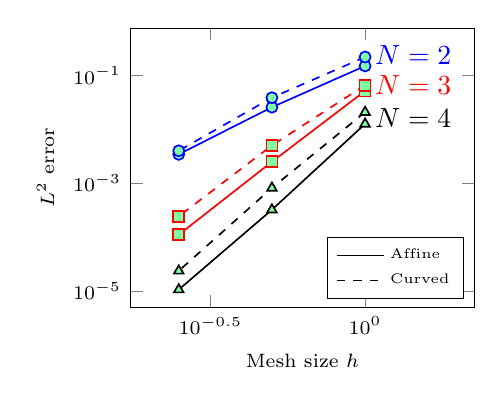
\begin{tikzpicture}
\begin{loglogaxis}[
    legend cell align=left,
    legend style={legend pos=south east, font=\tiny},
    width=.49\textwidth,    
    xlabel={Mesh size $h$},
    ylabel={$L^2$ error}, 
     ymin=5e-6, ymax=.75,    
     xmin=1.75e-1, xmax=2.25,         
    grid style=dashed,
    legend entries={Affine,Curved}
] 
\addlegendimage{no markers,black}
\addlegendimage{no markers,dashed,black}

\addplot[color=blue,mark=*,semithick, mark options={solid,fill=markercolor}]
coordinates{(1,0.149639)(0.5,0.025693)(0.25,0.00342827)} [yshift=4pt] node[right, pos=0, color=blue] {$N = 2$};
\addplot[color=blue,mark=*,dashed,semithick, mark options={solid,fill=markercolor}]
coordinates{(1,0.219501)(0.5,0.0385896)(0.25,0.0039906)};
\logLogSlopeTriangleFlip{0.285}{0.15}{0.6}{3}{blue}


\addplot[color=red,mark=square*,semithick, mark options={solid,fill=markercolor}]
coordinates{(1,0.0516053)(0.5,0.00249425)(0.25,0.000110618)}[yshift=2pt] node[right, pos=0, color=red] {$N = 3$};
\addplot[color=red,mark=square*,dashed,semithick, mark options={solid,fill=markercolor}]
coordinates{(1,0.0657418)(0.5,0.00501536)(0.25,0.000243005)};
\logLogSlopeTriangleFlip{0.285}{0.15}{0.36}{4}{red}

\addplot[color=black,mark=triangle*,semithick, mark options={solid,fill=markercolor}]
coordinates{(1,0.0125714)(0.5,0.000321559)(0.25,1.06097e-05)} [yshift=2pt] node[right, pos=0, color=black] {$N = 4$};
\addplot[color=black,mark=triangle*,dashed,semithick, mark options={solid,fill=markercolor}]
coordinates{(1,0.0207604)(0.5,0.000816006)(0.25,2.36102e-05)};
\logLogSlopeTriangle{0.31}{0.15}{0.05}{5}{black}

%\legend{$L^2$ projection,Weight-adjusted,Difference}
%\legend{Uniform, Optimal, Smoothed}
\end{loglogaxis}
\end{tikzpicture}}
\hspace{.5em}
\subfloat[3D results]{
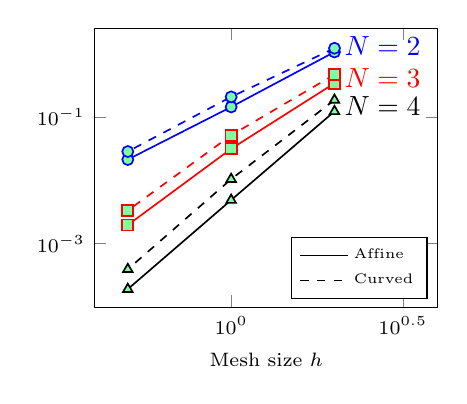
\begin{tikzpicture}
\begin{loglogaxis}[
    legend cell align=left,
    legend style={legend pos=south east, font=\tiny},
    width=.49\textwidth,    
    xlabel={Mesh size $h$},
%    ylabel={$L^2$ error}, 
     ymin=1e-4, ymax=2.5,    
     xmin=4e-1, xmax=4,         
    grid style=dashed,
    legend entries={Affine,Curved}
] 
\addlegendimage{no markers,black}
\addlegendimage{no markers,dashed,black}

\addplot[color=blue,mark=*,semithick, mark options={solid,fill=markercolor}]
coordinates{(2,1.05519)(1,0.143515)(0.5,0.0212682)}[yshift=2pt] node[right, pos=.0, color=blue] {$N = 2$};
\addplot[color=blue,mark=*,dashed,semithick, mark options={solid,fill=markercolor}]
coordinates{(2,1.20915)(1,0.2069)(0.5,0.0284505)};
\logLogSlopeTriangleFlip{0.25}{0.125}{0.6}{3}{blue}

\addplot[color=red,mark=square*,semithick, mark options={solid,fill=markercolor}]
coordinates{(2,0.339318)(1,0.0314342)(0.5,0.00197699)}[yshift=2pt] node[right, pos=0, color=red] {$N = 3$};
\addplot[color=red,mark=square*,dashed,semithick, mark options={solid,fill=markercolor}]
coordinates{(2,0.464613)(1,0.0513369)(0.5,0.00334595)};
\logLogSlopeTriangleFlip{0.25}{0.125}{0.39}{4}{red}

\addplot[color=black,mark=triangle*,semithick, mark options={solid,fill=markercolor}]
coordinates{(2,0.122229)(1,0.00488434)(0.5,0.000192453)}[yshift=2pt] node[right, pos=0, color=black] {$N = 4$};
\addplot[color=black,mark=triangle*,dashed,semithick, mark options={solid,fill=markercolor}]
coordinates{(2,0.184547)(1,0.0104361)(.5,0.0003960681)};
\logLogSlopeTriangle{0.25}{0.125}{0.05}{5}{black}

%\legend{$L^2$ projection,Weight-adjusted,Difference}
%\legend{Uniform, Optimal, Smoothed}
\end{loglogaxis}
\end{tikzpicture}}


\caption*{$L^2$ errors for 2D/3D isentropic vortex at $T=5$ on affine, curved meshes.}
}
\end{figure}
\only<1>{
\vspace{-.5em}
\begin{itemize}
\item Entropy stability: needs discrete geometric conservation law (GCL).
\item Generalized ``weight-adjusted'' mass lumping for curved meshes.
\item Modify $\tilde{\bm{u}} = \bm{u}\LRp{\tilde{\bm{v}}}$, $\tilde{\bm{v}} = \tilde{P}_N^k\bm{v}(\bm{u}_h)$ using weight-adjusted projection $\tilde{P}^k_N$.
\end{itemize}
}

\let\thefootnote\relax\footnotetext{\tiny Visbal and Gaitonde (2002).  On the Use of Higher-Order Finite-Difference
Schemes on Curvilinear and Deforming Meshes.}
\let\thefootnote\relax\footnotetext{\tiny Kopriva (2006).  Metric identities and the discontinuous spectral element method on curvilinear meshes.}
\let\thefootnote\relax\footnotetext{\tiny Chan, Hewett, and Warburton (2016). \textit{Weight-adjusted discontinuous Galerkin methods: curvilinear meshes}.}
%\let\thefootnote\relax\footnotetext{\tiny Chan, Wilcox (2018). \textit{On discretely entropy stable weight-adjusted DG methods: curvilinear meshes}.}
}

%\frame{
%\frametitle{2D curved meshes: conservation of entropy}
%
%\begin{figure}
%\centering
%\subfloat[With weight-adjusted projection]{
%\begin{tikzpicture}
%\begin{semilogyaxis}[
%    legend cell align=left,
%    legend style={legend pos=south east, font=\tiny},
%    width=.48\textwidth,    
%    xlabel={Time $t$},
%    ylabel={Change in entropy $\Delta U(\bm{u})$}, 
%     ymin=1e-9, ymax=5e-4,    
%    grid style=dashed,
%] 
%
%\addplot[color=blue,mark=*,semithick, mark options={solid,fill=markercolor}]
%coordinates{(0.025641,0)(0.128205,1.81455e-05)(0.230769,1.84993e-05)(0.333333,1.81016e-05)(0.435897,2.38212e-05)(0.538462,3.43804e-05)(0.641026,3.75077e-05)(0.74359,3.80509e-05)(0.846154,4.02406e-05)(0.948718,4.57864e-05)(1.05128,5.21023e-05)(1.15385,5.52339e-05)(1.25641,5.93653e-05)(1.35897,6.53204e-05)(1.46154,7.10508e-05)(1.5641,7.58692e-05)(1.66667,8.21148e-05)(1.76923,8.86933e-05)(1.87179,9.52306e-05)(1.97436,0.000102832)};
%%\addplot[color=blue,dashed,semithick, mark options={solid,fill=markercolor}]
%%coordinates{(0.025641,9.95731e-16)(0.128205,4.11303e-15)(0.230769,1.09496e-14)(0.333333,1.86934e-14)(0.435897,1.8624e-14)(0.538462,4.82253e-14)(0.641026,2.80886e-14)(0.74359,3.34073e-14)(0.846154,3.41116e-14)(0.948718,1.12826e-14)(1.05128,1.02106e-14)(1.15385,7.27543e-15)(1.25641,3.21965e-15)(1.35897,2.70617e-15)(1.46154,2.28116e-15)(1.5641,1.01134e-14)(1.66667,9.05179e-15)(1.76923,8.96852e-15)(1.87179,2.69368e-14)(1.97436,1.20043e-15)};
%\addplot[color=red,mark=square*,semithick, mark options={solid,fill=markercolor}]
%coordinates{(0.0129032,0)(0.116129,9.54018e-07)(0.219355,8.64409e-07)(0.322581,7.28292e-07)(0.425806,1.00547e-06)(0.529032,1.54507e-06)(0.632258,1.58376e-06)(0.735484,1.48926e-06)(0.83871,1.52599e-06)(0.941935,1.77263e-06)(1.04516,2.04306e-06)(1.14839,2.10785e-06)(1.25161,2.25231e-06)(1.35484,2.49471e-06)(1.45806,2.7075e-06)(1.56129,2.86391e-06)(1.66452,3.11015e-06)(1.76774,3.35711e-06)(1.87097,3.6045e-06)(1.97419,3.88568e-06)};
%%\addplot[color=red,dotted,semithick, mark options={solid,fill=markercolor}]
%%coordinates{(0.0129032,1.00787e-15)(0.116129,2.48065e-16)(0.219355,8.43769e-15)(0.322581,1.07483e-14)(0.425806,6.18255e-15)(0.529032,4.95159e-14)(0.632258,1.19835e-14)(0.735484,3.68837e-14)(0.83871,2.35957e-14)(0.941935,1.19904e-14)(1.04516,1.73785e-14)(1.14839,7.88952e-15)(1.25161,2.44249e-14)(1.35484,6.38031e-15)(1.45806,1.78781e-14)(1.56129,5.72459e-16)(1.66452,4.02456e-15)(1.76774,1.7316e-14)(1.87097,2.50425e-14)(1.97419,3.55375e-14)};
%\addplot[color=black,mark=pentagon*,semithick, mark options={solid,fill=markercolor}]
%coordinates{(0.00647249,0)(0.110032,5.38994e-08)(0.213592,4.43651e-08)(0.317152,3.18878e-08)(0.420712,4.65967e-08)(0.524272,7.64772e-08)(0.627832,7.36288e-08)(0.731392,6.33475e-08)(0.834951,6.22881e-08)(0.938511,7.43794e-08)(1.04207,8.71374e-08)(1.14563,8.67872e-08)(1.24919,9.19998e-08)(1.35275,1.02781e-07)(1.45631,1.11204e-07)(1.55987,1.16121e-07)(1.66343,1.26634e-07)(1.76699,1.36562e-07)(1.87055,1.46567e-07)(1.97411,1.57581e-07)};
%%\addplot[color=black,dashdotted,semithick, mark options={solid,fill=markercolor}]
%%coordinates{(0.00647249,2.19226e-16)(0.110032,5.88071e-15)(0.213592,1.34059e-14)(0.317152,2.30337e-14)(0.420712,8.23647e-15)(0.524272,2.68709e-14)(0.627832,2.53304e-14)(0.731392,2.95527e-14)(0.834951,2.5948e-14)(0.938511,4.56579e-15)(1.04207,2.28428e-14)(1.14563,8.22259e-15)(1.24919,1.51094e-14)(1.35275,7.86871e-15)(1.45631,1.11508e-14)(1.55987,1.57721e-14)(1.66343,6.95624e-15)(1.76699,2.07681e-14)(1.87055,2.72421e-14)(1.97411,1.7028e-14)};
%
%% % N = 4, K= 8, dt = .25
% % N = 4, K= 8, dt = .125
% % N = 4, K= 8, dt = .0625
%
%%\legend{${\rm CFL} = .25$,${\rm CFL} = .125$,${\rm CFL} = .0625$ }
%%\legend{Uniform, Optimal, Smoothed}
%\end{semilogyaxis}
%\end{tikzpicture}
%}
%\subfloat[Without weight-adjusted projection]{
%\begin{tikzpicture}
%\begin{semilogyaxis}[
%    legend cell align=left,
%    legend style={legend pos=south east, font=\tiny},
%    width=.48\textwidth,
%    xlabel={Time $t$},
%%         ymin=1e-10, ymax=1e-1,    
%%     ymin=1e-7, ymax=1e1,
%     ymin=1e-9, ymax=5e-4,    
%%    ylabel={$L^2$ error}, 
%    grid style=dashed,
%] 
%
%\addplot[color=blue,mark=*,semithick, mark options={solid,fill=markercolor}]
%coordinates{(0.025641,0)(0.128205,4.45681e-05)(0.230769,6.82313e-05)(0.333333,0.000131517)(0.435897,0.000108761)(0.538462,8.51562e-05)(0.641026,2.94791e-05)(0.74359,3.62904e-05)(0.846154,2.97564e-05)(0.948718,9.87886e-05)(1.05128,0.000136806)(1.15385,7.64601e-05)(1.25641,0.000111044)(1.35897,5.72761e-05)(1.46154,4.27e-05)(1.5641,5.03819e-05)(1.66667,4.99789e-05)(1.76923,5.07438e-05)(1.87179,4.26361e-05)(1.97436,2.48694e-05)};
%%\addplot[color=blue,dashed,semithick, mark options={solid,fill=markercolor}]
%%coordinates{(0.025641,5.11743e-16)(0.128205,1.16547e-14)(0.230769,7.91034e-15)(0.333333,1.28231e-14)(0.435897,4.79131e-15)(0.538462,3.44134e-14)(0.641026,6.92502e-15)(0.74359,2.28047e-14)(0.846154,2.15314e-14)(0.948718,4.36456e-15)(1.05128,2.09416e-14)(1.15385,4.86763e-15)(1.25641,3.59088e-15)(1.35897,3.43475e-16)(1.46154,1.03632e-14)(1.5641,1.03598e-14)(1.66667,1.83881e-16)(1.76923,5.94663e-15)(1.87179,3.18252e-14)(1.97436,1.88495e-14)};
%\addplot[color=red,mark=square*,semithick, mark options={solid,fill=markercolor}]
%coordinates{(0.0129032,0)(0.116129,6.48664e-05)(0.219355,8.24474e-05)(0.322581,0.000152373)(0.425806,0.000138342)(0.529032,0.000126709)(0.632258,1.85501e-05)(0.735484,6.98555e-05)(0.83871,7.53129e-05)(0.941935,0.00013915)(1.04516,0.000196476)(1.14839,0.000133645)(1.25161,0.000173751)(1.35484,0.000126668)(1.45806,0.000116008)(1.56129,0.000127919)(1.66452,0.0001343)(1.76774,0.000140992)(1.87097,0.00013971)(1.97419,0.0001291)};
%%\addplot[color=red,dotted,semithick, mark options={solid,fill=markercolor}]
%%coordinates{(0.0129032,3.00107e-16)(0.116129,6.93196e-15)(0.219355,1.00198e-14)(0.322581,7.79932e-15)(0.425806,2.48759e-15)(0.529032,3.46181e-14)(0.632258,1.7205e-14)(0.735484,2.30718e-14)(0.83871,3.0146e-14)(0.941935,9.4369e-15)(1.04516,1.07969e-14)(1.14839,5.59275e-15)(1.25161,5.34295e-15)(1.35484,5.7801e-15)(1.45806,8.74648e-15)(1.56129,1.24137e-14)(1.66452,2.95597e-15)(1.76774,2.64441e-14)(1.87097,2.58023e-14)(1.97419,6.984e-15)};
%\addplot[color=black,mark=pentagon*,semithick, mark options={solid,fill=markercolor}]
%coordinates{(0.00647249,0)(0.110032,6.52844e-05)(0.213592,8.08628e-05)(0.317152,0.000153077)(0.420712,0.000141625)(0.524272,0.000130883)(0.627832,2.58046e-05)(0.731392,6.81127e-05)(0.834951,7.92926e-05)(0.938511,0.000137768)(1.04207,0.000201777)(1.14563,0.000136705)(1.24919,0.000177364)(1.35275,0.000131153)(1.45631,0.000119851)(1.55987,0.000131686)(1.66343,0.000138676)(1.76699,0.00014539)(1.87055,0.000144608)(1.97411,0.000134142)};
%%\addplot[color=black,dashdotted,semithick, mark options={solid,fill=markercolor}]
%%coordinates{(0.00647249,7.31403e-16)(0.110032,1.05055e-14)(0.213592,2.58127e-15)(0.317152,1.04916e-14)(0.420712,5.12437e-15)(0.524272,4.40203e-14)(0.627832,1.147e-14)(0.731392,2.81025e-14)(0.834951,3.01946e-14)(0.938511,4.51028e-15)(1.04207,1.096e-14)(1.14563,6.11317e-15)(1.24919,3.69843e-15)(1.35275,6.47399e-15)(1.45631,9.41608e-15)(1.55987,1.58901e-15)(1.66343,6.39766e-15)(1.76699,1.56819e-14)(1.87055,2.11949e-14)(1.97411,1.12063e-14)};
%
%%\legend{Geo-$(N+1)$, $h^{N+2}$, Geo-$N$, $h^{N+1}$}
%\legend{${\rm CFL} = .25$,${\rm CFL} = .125$,${\rm CFL} = .0625$ }
%\end{semilogyaxis}
%\end{tikzpicture}
%}
%%\subfloat[Convergence of $\Delta S(\bm{u})$]{
%%\begin{tikzpicture}
%%\begin{loglogaxis}[
%%    legend cell align=left,
%%    legend style={legend pos=south east, font=\tiny},
%%    width=.475\textwidth,    
%%    xlabel={Mesh size $h$},
%%    ylabel={$L^2$ error}, 
%%     ymin=5e-6, ymax=2,    
%%     xmin=1e-1, xmax=2.5,         
%%    grid style=dashed,
%%    legend entries={Affine,Curved}
%%] 
%%\addlegendimage{no markers,black}
%%\addlegendimage{no markers,dashed,black}
%%
%%\addplot[color=blue,mark=*,semithick, mark options={solid,fill=markercolor}]
%%coordinates{(2,1.06717)(1,0.149639)(0.5,0.025693)(0.25,0.00342827)} [yshift=4pt] node[left, pos=1.05, color=blue] {$N = 2$};
%%\logLogSlopeTriangleFlip{0.45}{0.15}{0.575}{3}{blue}
%%
%%
%%%\legend{$L^2$ projection,Weight-adjusted,Difference}
%%%\legend{Uniform, Optimal, Smoothed}
%%\end{loglogaxis}
%%\end{tikzpicture}
%%}
%\caption{Change in entropy under an entropy conservative flux with $N=4$.  In both cases, the spatial formulation tested with $\tilde{\bm{v}} = P_N\bm{v}(\bm{u})$ is $O\LRp{10^{-14}}$. }
%%\label{fig:dSconverge}
%\end{figure}
%}

%\frame{
%\frametitle{3D isentropic vortex} 
%\begin{figure}
%\centering
%\subfloat[Affine mesh for $h = 1/2$]{\raisebox{2em}{\includegraphics[width=.425\textwidth]{figs/periodicCube3.png}}\label{subfig:mesh3d}}
%\subfloat[$L^2$ errors]{\begin{tikzpicture}
%\begin{loglogaxis}[
%    legend cell align=left,
%    legend style={legend pos=south east, font=\tiny},
%    width=.55\textwidth,    
%    xlabel={Mesh size $h$},
%    ylabel={$L^2$ error}, 
%     ymin=1e-4, ymax=2,    
%     xmin=4e-1, xmax=4,         
%    grid style=dashed,
%    legend entries={Affine,Curved}
%] 
%\addlegendimage{no markers,black}
%\addlegendimage{no markers,dashed,black}
%
%\addplot[color=blue,mark=*,semithick, mark options={solid,fill=markercolor}]
%coordinates{(2,1.05519)(1,0.143515)(0.5,0.0212682)}[yshift=2pt] node[right, pos=.0, color=blue] {$N = 2$};
%\addplot[color=blue,mark=*,dashed,semithick, mark options={solid,fill=markercolor}]
%coordinates{(2,1.20915)(1,0.2069)(0.5,0.0284505)};
%\logLogSlopeTriangle{0.25}{0.125}{0.525}{3}{blue}
%
%\addplot[color=red,mark=square*,semithick, mark options={solid,fill=markercolor}]
%coordinates{(2,0.339318)(1,0.0314342)(0.5,0.00197699)}[yshift=2pt] node[right, pos=0, color=red] {$N = 3$};
%\addplot[color=red,mark=square*,dashed,semithick, mark options={solid,fill=markercolor}]
%coordinates{(2,0.464613)(1,0.0513369)(0.5,0.00334595)};
%\logLogSlopeTriangle{0.25}{0.125}{0.3}{4}{red}
%
%\addplot[color=black,mark=triangle*,semithick, mark options={solid,fill=markercolor}]
%coordinates{(2,0.122229)(1,0.00488434)(0.5,0.000192453)}[yshift=2pt] node[right, pos=0, color=black] {$N = 4$};
%\addplot[color=black,mark=triangle*,dashed,semithick, mark options={solid,fill=markercolor}]
%coordinates{(2,0.184547)(1,0.0104361)(.5,0.0003960681)};
%\logLogSlopeTriangle{0.25}{0.125}{0.05}{5}{black}
%
%%\legend{$L^2$ projection,Weight-adjusted,Difference}
%%\legend{Uniform, Optimal, Smoothed}
%\end{loglogaxis}
%\end{tikzpicture}}
%\caption{$L^2$ errors at $T=5$ for the 3D isentropic vortex on affine, curved meshes.}
%\label{fig:converge3d}
%\end{figure}
%}
\frame{
\frametitle{2D Riemann problem}
\setcounter{subfigure}{0}

\begin{itemize}
\item Uniform $64\times 64$ mesh: $N=3$, CFL $.125$, Lax-Friedrichs stabilization.
\item No limiting or artificial viscosity required to maintain stability!
\item Periodic on larger domain (``natural'' boundary conditions unstable).
\end{itemize}
\vspace{-1em}
\begin{figure}
\centering
\subfloat[$\Omega = \LRs{-1,1}^2$]{\includegraphics[width=.425\textwidth]{figs/riemannBig.png}}
\hspace{2em}
\subfloat[$\Omega =\LRs{-.5,.5}^2$, $32\times 32$ elements]{\includegraphics[width=.425\textwidth]{figs/riemannSmall.png}}
\end{figure}
}


\frame{
\frametitle{Inviscid Taylor-Green vortex} 
%\vspace{-1em}
\begin{figure}
\centering
\includegraphics[width=.65\textwidth]{figs/taylorgreen.png}
\caption{Isocontours of $z$-vorticity for Taylor-Green at $t = 0, 10$ seconds.}
\end{figure}
%\vspace{-.5em}
\begin{itemize}
\item Simple turbulence-like behavior (generation of small scales).
%\vspace{.25em}
\item Inviscid Taylor-Green: tests robustness w.r.t.\ under-resolved solutions.
\end{itemize}
\let\thefootnote\relax\footnotetext{\tiny \url{https://how4.cenaero.be/content/bs1-dns-taylor-green-vortex-re1600}.}
}

\frame{
\frametitle{Taylor-Green vortex: kinetic energy dissipation rate} 
%\vspace{-.5em}
\begin{figure}
%\centering
%\only<1>{
%\subfloat[Kinetic energy ]{
%\begin{tikzpicture}
%\begin{axis}[
%        scaled ticks=false, 
%        tick label style={/pgf/number format/fixed},
%	legend cell align=left,
%	legend style={font=\tiny},
%	width=.475\textwidth,
%    xlabel={Time $t$},
%    ylabel={$\kappa(t)$},
%%    xmin=.005, xmax=1,
%%    ymin=1e-10, ymax=1e-1,
%    legend pos=north east,
%    xmajorgrids=true,
%    ymajorgrids=true,
%    grid style=dashed,
%%    ytick={0,.001, .005, .01, .015},
%%    yticklabels={$0$,$\frac{\pi}{2}$,$\pi$,$\frac{3\pi}{2}$},
%] 
%\addplot[color=blue,,semithick, mark options={fill=markercolor}]
%coordinates{(0,0.125)(0.178731,0.125)(0.357462,0.125002)(0.536193,0.125005)(0.714924,0.125009)(0.893655,0.125014)(1.07239,0.125018)(1.25112,0.125023)(1.42985,0.125027)(1.60858,0.125031)(1.78731,0.125034)(1.96604,0.125037)(2.14477,0.125039)(2.3235,0.12504)(2.50223,0.125039)(2.68097,0.125037)(2.8597,0.125032)(3.03843,0.125023)(3.21716,0.125008)(3.39589,0.124984)(3.57462,0.124942)(3.75335,0.124872)(3.93208,0.124756)(4.11081,0.124577)(4.28954,0.124315)(4.46828,0.123948)(4.64701,0.123461)(4.82574,0.122861)(5.00447,0.122182)(5.1832,0.12146)(5.36193,0.120701)(5.54066,0.119905)(5.71939,0.119069)(5.89812,0.118168)(6.07685,0.117182)(6.25558,0.1161)(6.43432,0.1149)(6.61305,0.113564)(6.79178,0.112093)(6.97051,0.110495)(7.14924,0.108768)(7.32797,0.106898)(7.5067,0.104859)(7.68543,0.10263)(7.86416,0.100247)(8.04289,0.0977593)(8.22163,0.0952161)(8.40036,0.092669)(8.57909,0.0901535)(8.75782,0.0876812)(8.93655,0.0852575)(9.11528,0.0828687)(9.29401,0.0804991)(9.47274,0.0781493)(9.65147,0.0758373)(9.83021,0.0735985)(10.0089,0.0714455)(10.1877,0.0693647)(10.3664,0.0673466)(10.5451,0.0653915)(10.7239,0.063496)(10.9026,0.0616565)(11.0813,0.0598745)(11.2601,0.0581523)(11.4388,0.0564894)(11.6175,0.0548814)(11.7962,0.0533217)(11.975,0.0518057)(12.1537,0.0503292)(12.3324,0.0488935)(12.5112,0.0475009)(12.6899,0.0461529)(12.8686,0.0448499)(13.0474,0.0435915)(13.2261,0.0423768)(13.4048,0.0412054)(13.5836,0.0400793)(13.7623,0.0390016)(13.941,0.0379701)(14.1197,0.0369793)(14.2985,0.0360246)(14.4772,0.0351027)(14.6559,0.0342115)(14.8347,0.0333479)(15.0134,0.032511)(15.1921,0.0317027)(15.3709,0.0309235)(15.5496,0.0301727)(15.7283,0.0294487)(15.9071,0.0287493)(16.0858,0.0280732)(16.2645,0.027421)(16.4433,0.0267929)(16.622,0.0261868)(16.8007,0.0256001)(16.9794,0.025031)(17.1582,0.0244798)(17.3369,0.023947)(17.5156,0.0234321)(17.6944,0.0229344)(17.8731,0.0224536)(18.0518,0.0219896)(18.2306,0.0215416)(18.4093,0.0211082)(18.588,0.0206882)(18.7668,0.02028)(18.9455,0.0198829)(19.1242,0.0194966)(19.3029,0.0191212)(19.4817,0.0187558)(19.6604,0.0184)(19.8391,0.0180542)};
%
%\addplot[color=red,dashed,semithick, mark options={fill=markercolor}]
%coordinates{(0,0.125)(0.18796,0.125)(0.37592,0.125002)(0.563879,0.125006)(0.751839,0.125009)(0.939799,0.125014)(1.12776,0.125019)(1.31572,0.125024)(1.50368,0.125028)(1.69164,0.125032)(1.8796,0.125035)(2.06756,0.125037)(2.25552,0.125038)(2.44348,0.125036)(2.63144,0.125032)(2.8194,0.125023)(3.00736,0.125009)(3.19532,0.124985)(3.38328,0.124947)(3.57124,0.124884)(3.7592,0.124781)(3.94716,0.124621)(4.13512,0.124379)(4.32308,0.124027)(4.51104,0.123541)(4.699,0.122909)(4.88696,0.122149)(5.07491,0.121302)(5.26288,0.120396)(5.45083,0.11944)(5.6388,0.118433)(5.82676,0.11736)(6.01471,0.116193)(6.20267,0.114912)(6.39063,0.113497)(6.57859,0.11193)(6.76655,0.110204)(6.95451,0.108334)(7.14247,0.106322)(7.33043,0.104189)(7.51839,0.101934)(7.70635,0.0995426)(7.89431,0.0970654)(8.08227,0.0945369)(8.27023,0.0919787)(8.45819,0.0894304)(8.64615,0.0868905)(8.83411,0.0843671)(9.02207,0.0818692)(9.21003,0.0794052)(9.39799,0.0769825)(9.58595,0.0746288)(9.77391,0.0723431)(9.96187,0.0701295)(10.1498,0.0679956)(10.3378,0.0659364)(10.5258,0.0639473)(10.7137,0.0620322)(10.9017,0.0601792)(11.0896,0.0583829)(11.2776,0.0566368)(11.4656,0.0549345)(11.6535,0.053277)(11.8415,0.0516697)(12.0294,0.0501198)(12.2174,0.0486301)(12.4053,0.047197)(12.5933,0.0458163)(12.7813,0.0444834)(12.9692,0.0431979)(13.1572,0.0419597)(13.3451,0.0407697)(13.5331,0.0396274)(13.7211,0.038527)(13.909,0.0374678)(14.097,0.0364487)(14.2849,0.0354663)(14.4729,0.034518)(14.6609,0.0336038)(14.8488,0.0327232)(15.0368,0.0318737)(15.2247,0.0310535)(15.4127,0.0302625)(15.6007,0.0295011)(15.7886,0.0287685)(15.9766,0.0280626)(16.1645,0.0273818)(16.3525,0.0267242)(16.5405,0.0260884)(16.7284,0.0254745)(16.9164,0.0248826)(17.1043,0.0243113)(17.2923,0.0237595)(17.4803,0.0232271)(17.6682,0.0227134)(17.8562,0.0222159)(18.0441,0.0217324)(18.2321,0.0212626)(18.4201,0.0208084)(18.608,0.0203709)(18.796,0.019949)(18.9839,0.0195411)(19.1719,0.0191457)(19.3599,0.0187618)(19.5478,0.0183882)(19.7358,0.0180246)(19.9237,0.0176713)};
%
%\legend{Affine, Curved}
%\end{axis}\end{tikzpicture}
%}
%\hspace{.25em}
%\subfloat[KE dissipation rate]{% ($N=3$, $h = {\pi}/ {8}$)]{
%\begin{tikzpicture}
%\begin{axis}[
%        scaled ticks=false, 
%        tick label style={/pgf/number format/fixed},
%	legend cell align=left,
%	legend style={font=\tiny},
%	width=.475\textwidth,
%    xlabel={Time $t$},
%    ylabel={$-\pd{\kappa}{t}$},
%%    xmin=.005, xmax=1,
%%    ymin=1e-10, ymax=1e-1,
%ymin=-.0025, ymax=.017,
%    legend pos=north east,
%    xmajorgrids=true,
%    ymajorgrids=true,
%    grid style=dashed,
%    ytick={0, .005, .01, .015},
%    yticklabels={0, .005, .01, .015}    
%] 
%\addplot[color=blue,semithick, mark options={fill=markercolor}]
%coordinates{(0.007149,-0)(0.207328,-1.12783e-05)(0.407507,-1.46618e-05)(0.607685,-2.53763e-05)(0.807864,-2.98876e-05)(1.00804,-2.65041e-05)(1.20822,-3.15793e-05)(1.4084,-2.48123e-05)(1.60858,-1.97371e-05)(1.80876,-2.42484e-05)(2.00894,-2.0301e-05)(2.20912,-1.40979e-05)(2.40929,-6.767e-06)(2.60947,1.12783e-05)(2.80965,2.98876e-05)(3.00983,6.31587e-05)(3.21001,0.000110528)(3.41019,0.000181581)(3.61037,0.000329891)(3.81054,0.00058027)(4.01072,0.000940613)(4.2109,0.00144081)(4.41108,0.00207803)(4.61126,0.00279816)(4.81144,0.00343031)(5.01162,0.00381377)(5.2118,0.00407881)(5.41197,0.00431791)(5.61215,0.00455532)(5.81233,0.00493822)(6.01251,0.00546492)(6.21269,0.00609087)(6.41287,0.00687415)(6.61305,0.00773299)(6.81323,0.00853827)(7.0134,0.00933057)(7.21358,0.010159)(7.41376,0.0111904)(7.61394,0.0123673)(7.81412,0.0132419)(8.0143,0.013865)(8.21448,0.0140928)(8.41466,0.0139739)(8.61483,0.0137714)(8.81501,0.0135272)(9.01519,0.0133541)(9.21537,0.0133011)(9.41555,0.0131477)(9.61573,0.0127451)(9.81591,0.012215)(10.0161,0.0117295)(10.2163,0.0113731)(10.4164,0.0110065)(10.6166,0.0106795)(10.8168,0.0103857)(11.017,0.0100281)(11.2172,0.00961873)(11.4173,0.00931591)(11.6175,0.00903677)(11.8177,0.0087441)(12.0179,0.00844409)(12.2181,0.00816101)(12.4182,0.0078689)(12.6184,0.00757115)(12.8186,0.00726438)(13.0188,0.00696776)(13.2189,0.00667621)(13.4191,0.00640158)(13.6193,0.00614162)(13.8195,0.0058918)(14.0197,0.00565214)(14.2198,0.00541755)(14.42,0.00519085)(14.6202,0.0049839)(14.8204,0.00477863)(15.0206,0.0045728)(15.2207,0.00437148)(15.4209,0.00419272)(15.6211,0.00402693)(15.8213,0.00386339)(16.0214,0.00371678)(16.2216,0.00359948)(16.4218,0.00349347)(16.622,0.00337222)(16.8222,0.00324083)(17.0223,0.00311451)(17.2225,0.00299835)(17.4227,0.00289571)(17.6229,0.00280323)(17.8231,0.00270906)(18.0232,0.00261432)(18.2234,0.00252071)(18.4236,0.00243612)(18.6238,0.00235717)(18.8239,0.00227371)(19.0241,0.00218913)(19.2243,0.00211187)(19.4245,0.00204025)(19.6247,0.00197089)(19.8248,0.00190548)};
%
%\addplot[color=red, dashed,semithick, mark options={fill=markercolor}]
%coordinates{(0.00662,-0)(0.20523,-1.01505e-05)(0.40384,-1.24062e-05)(0.60245,-2.31206e-05)(0.801059,-2.59402e-05)(0.999669,-2.31206e-05)(1.19828,-2.81958e-05)(1.39689,-2.19928e-05)(1.5955,-1.80453e-05)(1.79411,-2.14288e-05)(1.99272,-1.86093e-05)(2.19133,-1.63536e-05)(2.38994,-8.45875e-06)(2.58855,5.07525e-06)(2.78716,2.0301e-05)(2.98577,4.96247e-05)(3.18438,9.4738e-05)(3.38299,0.000160152)(3.5816,0.000283086)(3.78021,0.000504706)(3.97881,0.000825574)(4.17743,0.00126543)(4.37603,0.00183499)(4.57464,0.00247672)(4.77325,0.0030897)(4.97186,0.00349741)(5.17047,0.00375061)(5.36908,0.00398971)(5.56769,0.00419893)(5.7663,0.00449555)(5.96491,0.00496811)(6.16352,0.00551849)(6.36213,0.00618335)(6.56074,0.00695535)(6.75935,0.00776796)(6.95796,0.00847567)(7.15657,0.00922568)(7.35518,0.0102655)(7.55379,0.0113212)(7.7524,0.0122049)(7.95101,0.0127772)(8.14962,0.0130801)(8.34823,0.0132329)(8.54684,0.0131302)(8.74545,0.012815)(8.94406,0.0124564)(9.14267,0.0121327)(9.34128,0.0117836)(9.53989,0.0115276)(9.7385,0.0112761)(9.93711,0.0109236)(10.1357,0.0105819)(10.3343,0.0102689)(10.5329,0.0100225)(10.7315,0.00976309)(10.9302,0.00945689)(11.1288,0.00915857)(11.3274,0.00887436)(11.526,0.00861327)(11.7246,0.00831947)(11.9232,0.00802623)(12.1218,0.00775273)(12.3204,0.00746513)(12.519,0.00717584)(12.7176,0.00690742)(12.9163,0.00662038)(13.1149,0.00633448)(13.3135,0.00608184)(13.5121,0.00583767)(13.7107,0.00559631)(13.9093,0.00538653)(14.1079,0.00517958)(14.3065,0.00497093)(14.5051,0.00477976)(14.7037,0.00457393)(14.9024,0.00436246)(15.101,0.00417242)(15.2996,0.00400832)(15.4982,0.00385719)(15.6968,0.00370663)(15.8954,0.00355042)(16.094,0.00340831)(16.2926,0.00329102)(16.4912,0.00318557)(16.6898,0.00307729)(16.8884,0.00296056)(17.0871,0.00284214)(17.2857,0.00272597)(17.4843,0.00261714)(17.6829,0.00252353)(17.8815,0.00243725)(18.0801,0.00234984)(18.2787,0.00226413)(18.4773,0.00218349)(18.6759,0.0021051)(18.8745,0.00202954)(19.0732,0.00195848)(19.2718,0.00189589)(19.4704,0.00184288)(19.669,0.00179438)(19.8676,0.00174476)};
%
%\legend{Affine, Curved}
%\end{axis}\end{tikzpicture}
%}
%}
\only<1>{
%\subfloat[KE dissipation rate from Gassner, Winters, Kopriva (2016) ]{
%\includegraphics[width=.4\textwidth]{figs/gassner_dkedt.png}
%}
%\hspace{.25em}
%\subfloat[KE dissipation rate]{
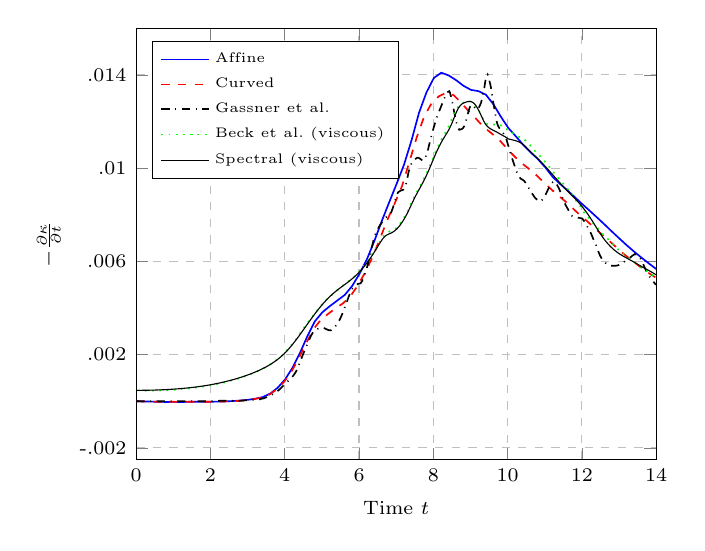
\begin{tikzpicture}
\begin{axis}[
        scaled ticks=false, 
        tick label style={/pgf/number format/fixed},
    legend pos=north west, 
    	legend cell align=left,
	legend style={font=\tiny},        
	width=.675\textwidth,
    xlabel={Time $t$},
    ylabel={$-\pd{\kappa}{t}$},
    xmin=0, xmax=14,
%    ymin=1e-10, ymax=1e-1,
ymin=-.0025, ymax=.016,
    xmajorgrids=true,
    ymajorgrids=true,
    grid style=dashed,
    ytick={-.002,  .002, .006,.01, .014},
    yticklabels={-.002,  .002, .006,.01,   .014}    
] 
\addplot[color=blue,semithick, mark options={fill=markercolor}]
coordinates{(0.007149,-0)(0.207328,-1.12783e-05)(0.407507,-1.46618e-05)(0.607685,-2.53763e-05)(0.807864,-2.98876e-05)(1.00804,-2.65041e-05)(1.20822,-3.15793e-05)(1.4084,-2.48123e-05)(1.60858,-1.97371e-05)(1.80876,-2.42484e-05)(2.00894,-2.0301e-05)(2.20912,-1.40979e-05)(2.40929,-6.767e-06)(2.60947,1.12783e-05)(2.80965,2.98876e-05)(3.00983,6.31587e-05)(3.21001,0.000110528)(3.41019,0.000181581)(3.61037,0.000329891)(3.81054,0.00058027)(4.01072,0.000940613)(4.2109,0.00144081)(4.41108,0.00207803)(4.61126,0.00279816)(4.81144,0.00343031)(5.01162,0.00381377)(5.2118,0.00407881)(5.41197,0.00431791)(5.61215,0.00455532)(5.81233,0.00493822)(6.01251,0.00546492)(6.21269,0.00609087)(6.41287,0.00687415)(6.61305,0.00773299)(6.81323,0.00853827)(7.0134,0.00933057)(7.21358,0.010159)(7.41376,0.0111904)(7.61394,0.0123673)(7.81412,0.0132419)(8.0143,0.013865)(8.21448,0.0140928)(8.41466,0.0139739)(8.61483,0.0137714)(8.81501,0.0135272)(9.01519,0.0133541)(9.21537,0.0133011)(9.41555,0.0131477)(9.61573,0.0127451)(9.81591,0.012215)(10.0161,0.0117295)(10.2163,0.0113731)(10.4164,0.0110065)(10.6166,0.0106795)(10.8168,0.0103857)(11.017,0.0100281)(11.2172,0.00961873)(11.4173,0.00931591)(11.6175,0.00903677)(11.8177,0.0087441)(12.0179,0.00844409)(12.2181,0.00816101)(12.4182,0.0078689)(12.6184,0.00757115)(12.8186,0.00726438)(13.0188,0.00696776)(13.2189,0.00667621)(13.4191,0.00640158)(13.6193,0.00614162)(13.8195,0.0058918)(14.0197,0.00565214)(14.2198,0.00541755)(14.42,0.00519085)(14.6202,0.0049839)(14.8204,0.00477863)(15.0206,0.0045728)(15.2207,0.00437148)(15.4209,0.00419272)(15.6211,0.00402693)(15.8213,0.00386339)(16.0214,0.00371678)(16.2216,0.00359948)(16.4218,0.00349347)(16.622,0.00337222)(16.8222,0.00324083)(17.0223,0.00311451)(17.2225,0.00299835)(17.4227,0.00289571)(17.6229,0.00280323)(17.8231,0.00270906)(18.0232,0.00261432)(18.2234,0.00252071)(18.4236,0.00243612)(18.6238,0.00235717)(18.8239,0.00227371)(19.0241,0.00218913)(19.2243,0.00211187)(19.4245,0.00204025)(19.6247,0.00197089)(19.8248,0.00190548)};

\addplot[color=red, dashed,semithick, mark options={fill=markercolor}]
coordinates{(0.00662,-0)(0.20523,-1.01505e-05)(0.40384,-1.24062e-05)(0.60245,-2.31206e-05)(0.801059,-2.59402e-05)(0.999669,-2.31206e-05)(1.19828,-2.81958e-05)(1.39689,-2.19928e-05)(1.5955,-1.80453e-05)(1.79411,-2.14288e-05)(1.99272,-1.86093e-05)(2.19133,-1.63536e-05)(2.38994,-8.45875e-06)(2.58855,5.07525e-06)(2.78716,2.0301e-05)(2.98577,4.96247e-05)(3.18438,9.4738e-05)(3.38299,0.000160152)(3.5816,0.000283086)(3.78021,0.000504706)(3.97881,0.000825574)(4.17743,0.00126543)(4.37603,0.00183499)(4.57464,0.00247672)(4.77325,0.0030897)(4.97186,0.00349741)(5.17047,0.00375061)(5.36908,0.00398971)(5.56769,0.00419893)(5.7663,0.00449555)(5.96491,0.00496811)(6.16352,0.00551849)(6.36213,0.00618335)(6.56074,0.00695535)(6.75935,0.00776796)(6.95796,0.00847567)(7.15657,0.00922568)(7.35518,0.0102655)(7.55379,0.0113212)(7.7524,0.0122049)(7.95101,0.0127772)(8.14962,0.0130801)(8.34823,0.0132329)(8.54684,0.0131302)(8.74545,0.012815)(8.94406,0.0124564)(9.14267,0.0121327)(9.34128,0.0117836)(9.53989,0.0115276)(9.7385,0.0112761)(9.93711,0.0109236)(10.1357,0.0105819)(10.3343,0.0102689)(10.5329,0.0100225)(10.7315,0.00976309)(10.9302,0.00945689)(11.1288,0.00915857)(11.3274,0.00887436)(11.526,0.00861327)(11.7246,0.00831947)(11.9232,0.00802623)(12.1218,0.00775273)(12.3204,0.00746513)(12.519,0.00717584)(12.7176,0.00690742)(12.9163,0.00662038)(13.1149,0.00633448)(13.3135,0.00608184)(13.5121,0.00583767)(13.7107,0.00559631)(13.9093,0.00538653)(14.1079,0.00517958)(14.3065,0.00497093)(14.5051,0.00477976)(14.7037,0.00457393)(14.9024,0.00436246)(15.101,0.00417242)(15.2996,0.00400832)(15.4982,0.00385719)(15.6968,0.00370663)(15.8954,0.00355042)(16.094,0.00340831)(16.2926,0.00329102)(16.4912,0.00318557)(16.6898,0.00307729)(16.8884,0.00296056)(17.0871,0.00284214)(17.2857,0.00272597)(17.4843,0.00261714)(17.6829,0.00252353)(17.8815,0.00243725)(18.0801,0.00234984)(18.2787,0.00226413)(18.4773,0.00218349)(18.6759,0.0021051)(18.8745,0.00202954)(19.0732,0.00195848)(19.2718,0.00189589)(19.4704,0.00184288)(19.669,0.00179438)(19.8676,0.00174476)};

\addplot[smooth,color=black,dashdotted,semithick, mark options={solid,fill=markercolor}]
  coordinates{(0.0,0) (0.28719,0) (0.53378,0) (0.78906,0) (1.04434,0) (1.29963,0) (1.54041,0) (1.80439,0) (2.05097,6.28e-06) (2.29755,2.197e-05) (2.54994,2.51e-05) (2.79942,2.51e-05) (3.0518,5.334e-05) (3.30709,7.845e-05) (3.54206,0.00019141) (3.80025,0.00042989) (4.04112,0.00079443) (4.28761,0.00123005) (4.53129,0.00216199) (4.76046,0.00295274) (5.00705,0.0031567) (5.25073,0.00304373) (5.4857,0.00352069) (5.73518,0.0045405) (5.75839,0.00465815) (5.82703,0.0048383) (5.90054,0.00495156) (5.97306,0.00503628) (6.03978,0.00505511) (6.08399,0.0051618) (6.20804,0.00570151) (6.43722,0.00715434) (6.7041,0.0078635) (6.82884,0.00798902) (6.91587,0.00831222) (7.04932,0.00895862) (7.18856,0.00906844) (7.25238,0.00924417) (7.2988,0.00955481) (7.33941,0.00986546) (7.40033,0.01016356) (7.57149,0.01044911) (7.73394,0.01032987) (7.83838,0.01067503) (7.88479,0.01098255) (7.93701,0.01129633) (7.98632,0.01160384) (8.10816,0.01222828) (8.33444,0.01312257) (8.42884,0.01330112) (8.46259,0.0131414) (8.49792,0.0129375) (8.61293,0.01200549) (8.68835,0.01169798) (8.70286,0.01164464) (8.8305,0.01179212) (9.01027,0.01269896) (9.1776,0.01250441) (9.28595,0.01280565) (9.32366,0.01310688) (9.37298,0.01343008) (9.40199,0.0137376) (9.46291,0.01401373) (9.49482,0.01383173) (9.54414,0.01352108) (9.59055,0.0130504) (9.65727,0.0124291) (9.7385,0.01182663) (9.92706,0.01139674) (9.99668,0.01108296) (10.08661,0.01059345) (10.20845,0.01000981) (10.23746,0.00986233) (10.3448,0.00955795) (10.43763,0.00946695) (10.50435,0.0093132) (10.67261,0.00888017) (10.73063,0.00874211) (10.88438,0.00856952) (11.02362,0.00886135) (11.11935,0.00918141) (11.2528,0.0094293) (11.37754,0.00914689) (11.45006,0.00885507) (11.52549,0.00853501) (11.62122,0.00824946) (11.73436,0.00795136) (11.84169,0.00787919) (12.00995,0.0078384) (12.11148,0.00757796) (12.21881,0.00729555) (12.30004,0.00698804) (12.38417,0.00668994) (12.45379,0.00638243) (12.54372,0.00609688) (12.72068,0.00583644) (12.97596,0.00583016) (13.20514,0.00605609) (13.2963,0.0061533) (13.42754,0.00631269) (13.54745,0.00619729) (13.64608,0.00590233) (13.73021,0.00559796) (13.84045,0.00530928) (13.97389,0.00503314) (13.9913,0.00499504)};

\addplot[smooth,color=green,dotted,semithick, mark options={solid,fill=markercolor}]
  coordinates{(0.0431,0.00046572) (0.14512,0.00046378) (0.24274,0.00044948) (0.34477,0.00046966) (0.44855,0.00045406) (0.52595,0.00046448) (0.61302,0.00045994) (0.73087,0.00048012) (0.8241,0.00046777) (0.9657,0.00049706) (1.02463,0.00049186) (1.15303,0.000514) (1.34213,0.00054719) (1.42304,0.0005498) (1.75814,0.00062335) (1.81091,0.00063311) (1.92612,0.0006767) (1.98945,0.00068387) (2.09587,0.00072876) (2.17326,0.00073267) (2.29903,0.00080164) (2.37643,0.00080555) (2.50308,0.00087776) (2.57432,0.00089208) (2.69921,0.00096105) (2.76605,0.00097471) (2.86895,0.00105928) (2.91996,0.00106189) (3.03166,0.00113736) (3.08531,0.00115883) (3.17326,0.00122909) (3.26209,0.00128569) (3.3905,0.00138717) (3.49428,0.00146459) (3.62093,0.00158754) (3.67898,0.00164348) (3.79595,0.0017918) (3.94283,0.001985) (4.13105,0.00230569) (4.1759,0.0023987) (4.3219,0.00269532) (4.36588,0.00281045) (4.53914,0.00320139) (4.79683,0.00374584) (5.07124,0.00427923) (5.13369,0.0043677) (5.19349,0.00447178) (5.27792,0.00457976) (5.31223,0.00463375) (5.3518,0.00470075) (5.41425,0.0047632) (5.48373,0.00486143) (5.54793,0.00494144) (5.58751,0.00498242) (5.70888,0.00512293) (5.77221,0.00521725) (5.85048,0.00530117) (5.86719,0.00533565) (6.03782,0.00559909) (6.10202,0.00572919) (6.16535,0.00587555) (6.20668,0.00595686) (6.24626,0.00603752) (6.3905,0.00639072) (6.44239,0.00651041) (6.58047,0.00690329) (6.66315,0.00708803) (6.76253,0.00723374) (6.82498,0.00728513) (6.90853,0.00733913) (6.99648,0.00742499) (7.04925,0.00751151) (7.15567,0.00774178) (7.23659,0.00795123) (7.31838,0.00815873) (7.36148,0.00831744) (7.4591,0.00867129) (7.56714,0.0090099) (7.5932,0.0090783) (7.63173,0.00918556) (7.65326,0.0092493) (7.67025,0.00930682) (7.68612,0.00935579) (7.69858,0.00939465) (7.71558,0.00944984) (7.73144,0.00950813) (7.75751,0.00958119) (7.78244,0.00965737) (7.80057,0.00972421) (7.82663,0.00980039) (7.84476,0.00987034) (7.87082,0.00996361) (7.89122,0.01003979) (7.91388,0.01011907) (7.93541,0.01021156) (7.95921,0.01030095) (7.97847,0.01037246) (7.99773,0.01044008) (8.01133,0.01049372) (8.0238,0.01054812) (8.04873,0.01064218) (8.06912,0.0107269) (8.08272,0.01077587) (8.10198,0.01085126) (8.13598,0.01096241) (8.15071,0.01102071) (8.17224,0.01109222) (8.19603,0.01117072) (8.2255,0.01125389) (8.24929,0.01132151) (8.27195,0.01138525) (8.30142,0.01146453) (8.32861,0.01153837) (8.35921,0.01162309) (8.38414,0.01169849) (8.42153,0.01181819) (8.45666,0.01195032) (8.48725,0.01206458) (8.51445,0.01217029) (8.54958,0.01232342) (8.5779,0.01242446) (8.60397,0.01249753) (8.64249,0.01257836) (8.66742,0.01262111) (8.69008,0.01265997) (8.71955,0.01270116) (8.74334,0.01273148) (8.77507,0.01276956) (8.8068,0.0128022) (8.83853,0.01282785) (8.86232,0.01284728) (8.88725,0.01287137) (8.91445,0.01288458) (8.94958,0.01287603) (8.96884,0.0128667) (8.99943,0.01285892) (9.0289,0.01284104) (9.04929,0.01281461) (9.06176,0.01278274) (9.08782,0.01273532) (9.11388,0.01269178) (9.13428,0.01265836) (9.15581,0.01263115) (9.17734,0.01259073) (9.1932,0.01255108) (9.20793,0.01250988) (9.22153,0.01247257) (9.23739,0.01243059) (9.24873,0.0123894) (9.26346,0.01235208) (9.27705,0.01231011) (9.29518,0.01225803) (9.31218,0.01219895) (9.33258,0.01214065) (9.35297,0.01207613) (9.37224,0.01201628) (9.3983,0.01195486) (9.4255,0.01191056) (9.45156,0.01188179) (9.48102,0.01187324) (9.50935,0.01187012) (9.54561,0.01186468) (9.58074,0.01186545) (9.62946,0.011867) (9.65892,0.01187632) (9.70198,0.01189031) (9.73598,0.01188953) (9.77677,0.01186854) (9.82323,0.01183277) (9.86289,0.01179313) (9.89688,0.01175892) (9.92408,0.01172705) (9.94788,0.01169517) (9.99773,0.01165242) (10.04193,0.01162132) (10.08385,0.01158245) (10.10878,0.01154436) (10.14731,0.0115016) (10.16884,0.01147206) (10.19943,0.01143863) (10.23796,0.01140443) (10.28442,0.01136245) (10.31161,0.01133446) (10.35014,0.01130492) (10.38754,0.01128315) (10.41926,0.0112606) (10.44873,0.01123261) (10.46686,0.01120541) (10.49405,0.01116032) (10.51671,0.01112145) (10.54278,0.01108025) (10.56544,0.01104605) (10.58584,0.01101573) (10.59943,0.01099474) (10.60963,0.01097764) (10.6153,0.01095743) (10.63796,0.01092633) (10.66969,0.01086648) (10.69575,0.01081595) (10.71955,0.01076853) (10.74674,0.010718) (10.77734,0.01066903) (10.8136,0.01061461) (10.84193,0.01056408) (10.86912,0.01051822) (10.89972,0.01046147) (10.93371,0.01039695) (10.96431,0.01034098) (11.00963,0.01026791) (11.05269,0.01018784) (11.09915,0.01010311) (11.13768,0.01002615) (11.17847,0.00993753) (11.25552,0.00978206) (11.30085,0.00968956) (11.36317,0.00957529) (11.41643,0.00948045) (11.45609,0.00940815) (11.50255,0.00932342) (11.53994,0.00925735) (11.57394,0.00919516) (11.61133,0.00912442) (11.63399,0.009077) (11.66006,0.00902336) (11.66799,0.00900782) (11.80739,0.00867511) (11.95163,0.00838308) (12.05453,0.00810211) (12.13896,0.00796553) (12.24802,0.00773984) (12.34477,0.00756098) (12.57608,0.00714733) (12.65523,0.00703417) (12.80563,0.00678897) (12.90853,0.00661532) (13.02287,0.00643646) (13.11346,0.00632785) (13.28672,0.00612104) (13.40193,0.00598316) (13.49164,0.0058739) (13.65611,0.00568594) (13.84345,0.00548173) (14.1803,0.00508566) (14.26825,0.00500827) (14.40018,0.00484437) (14.62533,0.00464667) (14.81266,0.00451401) (14.98065,0.0043976) (15.09587,0.00432412) (15.17766,0.00427664) (15.36763,0.00416414) (15.54705,0.00404188) (15.65699,0.00395799) (15.81354,0.00383768) (15.96658,0.00372388) (16.09499,0.00361852) (16.21548,0.00352487) (16.45471,0.00333498) (16.60158,0.00325239) (16.70449,0.00317761) (16.84521,0.00309307) (17.04837,0.00296496) (17.33773,0.00278547) (17.62885,0.00262876) (17.83729,0.00251886) (18.10378,0.00237515) (18.37467,0.00222558) (18.68074,0.00208513) (19.01583,0.00195118) (19.2788,0.00186731) (19.7124,0.00175289) (19.99033,0.00170024)};
 
 \addplot[smooth,color=black,thin, mark options={solid,fill=markercolor}]
  coordinates{( 0.0 , 0.00046874284 ) ( 0.01 , 0.00046873893 ) ( 0.02 , 0.000468736 ) ( 0.03 , 0.000468742835 ) ( 0.04 , 0.000468759425 ) ( 0.05 , 0.000468785775 ) ( 0.06 , 0.000468821895 ) ( 0.07 , 0.000468867775 ) ( 0.08 , 0.000468923425 ) ( 0.09 , 0.00046898885 ) ( 0.1 , 0.000469064045 ) ( 0.11 , 0.00046914902 ) ( 0.12 , 0.000469243785 ) ( 0.13 , 0.000469348355001 ) ( 0.14 , 0.000469462715 ) ( 0.15 , 0.00046958689 ) ( 0.16 , 0.00046972089 ) ( 0.17 , 0.000469864715 ) ( 0.18 , 0.000470018395 ) ( 0.19 , 0.000470181925 ) ( 0.2 , 0.000470355319999 ) ( 0.21 , 0.000470538605001 ) ( 0.22 , 0.00047073179 ) ( 0.23 , 0.000470934885 ) ( 0.24 , 0.00047114791 ) ( 0.25 , 0.000471370885 ) ( 0.26 , 0.00047160383 ) ( 0.27 , 0.000471846755 ) ( 0.28 , 0.000472099685 ) ( 0.29 , 0.00047236265 ) ( 0.3 , 0.000472635655 ) ( 0.31 , 0.00047291873 ) ( 0.32 , 0.0004732119 ) ( 0.33 , 0.00047351519 ) ( 0.34 , 0.00047382862 ) ( 0.35 , 0.000474152215 ) ( 0.36 , 0.00047448601 ) ( 0.37 , 0.000474830025 ) ( 0.38 , 0.000475184285 ) ( 0.39 , 0.000475548825 ) ( 0.4 , 0.000475923674999 ) ( 0.41 , 0.00047630886 ) ( 0.42 , 0.000476704415 ) ( 0.43 , 0.000477110375 ) ( 0.44 , 0.00047752676 ) ( 0.45 , 0.000477953609999 ) ( 0.46 , 0.00047839097 ) ( 0.47 , 0.000478838865 ) ( 0.48 , 0.000479297325 ) ( 0.49 , 0.000479766395 ) ( 0.5 , 0.00048024611 ) ( 0.51 , 0.0004807365 ) ( 0.52 , 0.00048123762 ) ( 0.53 , 0.0004817495 ) ( 0.54 , 0.00048227217 ) ( 0.55 , 0.000482805685 ) ( 0.56 , 0.000483350085 ) ( 0.57 , 0.000483905405 ) ( 0.58 , 0.000484471689999 ) ( 0.59 , 0.000485048985 ) ( 0.6 , 0.000485637335 ) ( 0.61 , 0.000486236784999 ) ( 0.62 , 0.00048684738 ) ( 0.63 , 0.00048746916 ) ( 0.64 , 0.000488102175 ) ( 0.65 , 0.000488746475 ) ( 0.66 , 0.00048940211 ) ( 0.67 , 0.00049006913 ) ( 0.68 , 0.00049074757 ) ( 0.69 , 0.000491437495 ) ( 0.7 , 0.000492138955 ) ( 0.71 , 0.00049285199 ) ( 0.72 , 0.00049357666 ) ( 0.73 , 0.000494313015 ) ( 0.74 , 0.000495061115 ) ( 0.75 , 0.00049582101 ) ( 0.76 , 0.00049659275 ) ( 0.77 , 0.00049737639 ) ( 0.78 , 0.000498171995 ) ( 0.79 , 0.00049897961 ) ( 0.8 , 0.000499799295 ) ( 0.81 , 0.000500631115 ) ( 0.82 , 0.00050147512 ) ( 0.83 , 0.00050233137 ) ( 0.84 , 0.000503199925 ) ( 0.85 , 0.00050408085 ) ( 0.86 , 0.000504974195 ) ( 0.87 , 0.000505880025 ) ( 0.88 , 0.00050679841 ) ( 0.89 , 0.0005077294 ) ( 0.9 , 0.000508673065 ) ( 0.91 , 0.000509629465 ) ( 0.92 , 0.000510598665 ) ( 0.93 , 0.000511580735 ) ( 0.94 , 0.00051257573 ) ( 0.95 , 0.00051358372 ) ( 0.96 , 0.00051460477 ) ( 0.97 , 0.00051563895 ) ( 0.98 , 0.000516686325 ) ( 0.99 , 0.000517746965 ) ( 1.0 , 0.000518820935 ) ( 1.01 , 0.0005199083 ) ( 1.02 , 0.000521009145 ) ( 1.03 , 0.000522123525 ) ( 1.04 , 0.00052325151 ) ( 1.05 , 0.00052439319 ) ( 1.06 , 0.000525548615 ) ( 1.07 , 0.000526717860001 ) ( 1.08 , 0.00052790101 ) ( 1.09 , 0.00052909813 ) ( 1.1 , 0.00053030929 ) ( 1.11 , 0.000531534575 ) ( 1.12 , 0.000532774055 ) ( 1.13 , 0.0005340278 ) ( 1.14 , 0.00053529589 ) ( 1.15 , 0.000536578405 ) ( 1.16 , 0.00053787542 ) ( 1.17 , 0.00053918701 ) ( 1.18 , 0.00054051325 ) ( 1.19 , 0.000541854225 ) ( 1.2 , 0.000543210015001 ) ( 1.21 , 0.00054458069 ) ( 1.22 , 0.000545966339999 ) ( 1.23 , 0.000547367045 ) ( 1.24 , 0.000548782880001 ) ( 1.25 , 0.00055021393 ) ( 1.26 , 0.000551660279999 ) ( 1.27 , 0.000553122005 ) ( 1.28 , 0.00055459919 ) ( 1.29 , 0.000556091925 ) ( 1.3 , 0.000557600295 ) ( 1.31 , 0.000559124375 ) ( 1.32 , 0.000560664255 ) ( 1.33 , 0.00056222002 ) ( 1.34 , 0.00056379176 ) ( 1.35 , 0.00056537956 ) ( 1.36 , 0.000566983505 ) ( 1.37 , 0.000568603685 ) ( 1.38 , 0.00057024018 ) ( 1.39 , 0.00057189309 ) ( 1.4 , 0.000573562505 ) ( 1.41 , 0.000575248505 ) ( 1.42 , 0.000576951179999 ) ( 1.43 , 0.00057867063 ) ( 1.44 , 0.00058040694 ) ( 1.45 , 0.000582160205 ) ( 1.46 , 0.000583930515 ) ( 1.47 , 0.000585717955 ) ( 1.48 , 0.000587522635 ) ( 1.49 , 0.000589344635 ) ( 1.5 , 0.00059118405 ) ( 1.51 , 0.00059304098 ) ( 1.52 , 0.000594915515 ) ( 1.53 , 0.000596807755 ) ( 1.54 , 0.000598717795 ) ( 1.55 , 0.000600645725 ) ( 1.56 , 0.000602591645001 ) ( 1.57 , 0.00060455566 ) ( 1.58 , 0.000606537849999 ) ( 1.59 , 0.00060853833 ) ( 1.6 , 0.000610557195 ) ( 1.61 , 0.000612594535 ) ( 1.62 , 0.00061465046 ) ( 1.63 , 0.00061672506 ) ( 1.64 , 0.00061881844 ) ( 1.65 , 0.000620930705 ) ( 1.66 , 0.00062306195 ) ( 1.67 , 0.000625212275 ) ( 1.68 , 0.00062738179 ) ( 1.69 , 0.000629570589999 ) ( 1.7 , 0.000631778775 ) ( 1.71 , 0.000634006455 ) ( 1.72 , 0.00063625373 ) ( 1.73 , 0.000638520705 ) ( 1.74 , 0.000640807485 ) ( 1.75 , 0.00064311417 ) ( 1.76 , 0.000645440865 ) ( 1.77 , 0.00064778768 ) ( 1.78 , 0.00065015472 ) ( 1.79 , 0.00065254209 ) ( 1.8 , 0.00065494989 ) ( 1.81 , 0.00065737823 ) ( 1.82 , 0.000659827225 ) ( 1.83 , 0.000662296975 ) ( 1.84 , 0.000664787585 ) ( 1.85 , 0.000667299165 ) ( 1.86 , 0.000669831825 ) ( 1.87 , 0.00067238567 ) ( 1.88 , 0.000674960815 ) ( 1.89 , 0.000677557365 ) ( 1.9 , 0.000680175425 ) ( 1.91 , 0.00068281511 ) ( 1.92 , 0.000685476525 ) ( 1.93 , 0.00068815979 ) ( 1.94 , 0.000690865005 ) ( 1.95 , 0.00069359228 ) ( 1.96 , 0.00069634174 ) ( 1.97 , 0.00069911348 ) ( 1.98 , 0.000701907610001 ) ( 1.99 , 0.000704724260001 ) ( 2.0 , 0.00070756353 ) ( 2.01 , 0.000710425525 ) ( 2.02 , 0.000713310365 ) ( 2.03 , 0.000716218165 ) ( 2.04 , 0.000719149035 ) ( 2.05 , 0.000722103085 ) ( 2.06 , 0.000725080429999 ) ( 2.07 , 0.00072808118 ) ( 2.08 , 0.000731105455 ) ( 2.09 , 0.000734153369999 ) ( 2.1 , 0.00073722503 ) ( 2.11 , 0.000740320545 ) ( 2.12 , 0.00074344004 ) ( 2.13 , 0.00074658363 ) ( 2.14 , 0.000749751425001 ) ( 2.15 , 0.00075294354 ) ( 2.16 , 0.000756160085 ) ( 2.17 , 0.000759401180001 ) ( 2.18 , 0.00076266694 ) ( 2.19 , 0.00076595748 ) ( 2.2 , 0.000769272915 ) ( 2.21 , 0.000772613365 ) ( 2.22 , 0.00077597894 ) ( 2.23 , 0.00077936975 ) ( 2.24 , 0.00078278593 ) ( 2.25 , 0.000786227585 ) ( 2.26 , 0.00078969482 ) ( 2.27 , 0.000793187774999 ) ( 2.28 , 0.000796706555 ) ( 2.29 , 0.000800251275 ) ( 2.3 , 0.000803822065 ) ( 2.31 , 0.00080741903 ) ( 2.32 , 0.000811042285 ) ( 2.33 , 0.000814691965 ) ( 2.34 , 0.00081836818 ) ( 2.35 , 0.000822071044999 ) ( 2.36 , 0.00082580069 ) ( 2.37 , 0.000829557225 ) ( 2.38 , 0.00083334077 ) ( 2.39 , 0.00083715146 ) ( 2.4 , 0.000840989405 ) ( 2.41 , 0.000844854725 ) ( 2.42 , 0.00084874755 ) ( 2.43 , 0.000852667995 ) ( 2.44 , 0.000856616189999 ) ( 2.45 , 0.00086059226 ) ( 2.46 , 0.00086459633 ) ( 2.47 , 0.00086862852 ) ( 2.48 , 0.00087268896 ) ( 2.49 , 0.000876777775 ) ( 2.5 , 0.0008808951 ) ( 2.51 , 0.000885041065 ) ( 2.52 , 0.00088921579 ) ( 2.53 , 0.00089341941 ) ( 2.54 , 0.000897652065 ) ( 2.55 , 0.000901913885 ) ( 2.56 , 0.000906205005 ) ( 2.57 , 0.000910525565 ) ( 2.58 , 0.000914875695 ) ( 2.59 , 0.00091925554 ) ( 2.6 , 0.00092366524 ) ( 2.61 , 0.000928104945 ) ( 2.62 , 0.000932574795 ) ( 2.63 , 0.00093707493 ) ( 2.64 , 0.000941605515 ) ( 2.65 , 0.00094616669 ) ( 2.66 , 0.00095075861 ) ( 2.67 , 0.000955381435 ) ( 2.68 , 0.000960035325 ) ( 2.69 , 0.00096472044 ) ( 2.7 , 0.00096943694 ) ( 2.71 , 0.000974185 ) ( 2.72 , 0.000978964785 ) ( 2.73 , 0.00098377647 ) ( 2.74 , 0.00098862024 ) ( 2.75 , 0.00099349627 ) ( 2.76 , 0.00099840475 ) ( 2.77 , 0.001003345865 ) ( 2.78 , 0.00100831981 ) ( 2.79 , 0.001013326785 ) ( 2.8 , 0.001018366995 ) ( 2.81 , 0.001023440645 ) ( 2.82 , 0.00102854795 ) ( 2.83 , 0.001033689135 ) ( 2.84 , 0.00103886441 ) ( 2.85 , 0.00104407402 ) ( 2.86 , 0.0010493182 ) ( 2.87 , 0.00105459719 ) ( 2.88 , 0.00105991124 ) ( 2.89 , 0.001065260605 ) ( 2.9 , 0.00107064556 ) ( 2.91 , 0.00107606637 ) ( 2.92 , 0.00108152332 ) ( 2.93 , 0.0010870167 ) ( 2.94 , 0.001092546805 ) ( 2.95 , 0.00109811395 ) ( 2.96 , 0.001103718445 ) ( 2.97 , 0.00110936062 ) ( 2.98 , 0.00111504081 ) ( 2.99 , 0.00112075937 ) ( 3.0 , 0.001126516665 ) ( 3.01 , 0.001132313055 ) ( 3.02 , 0.00113814893 ) ( 3.03 , 0.00114402469 ) ( 3.04 , 0.00114994074 ) ( 3.05 , 0.00115589751 ) ( 3.06 , 0.001161895435 ) ( 3.07 , 0.00116793497 ) ( 3.08 , 0.00117401659 ) ( 3.09 , 0.00118014078 ) ( 3.1 , 0.00118630803 ) ( 3.11 , 0.00119251887 ) ( 3.12 , 0.001198773845 ) ( 3.13 , 0.001205073495 ) ( 3.14 , 0.00121141841 ) ( 3.15 , 0.00121780918 ) ( 3.16 , 0.001224246425 ) ( 3.17 , 0.00123073078 ) ( 3.18 , 0.00123726291 ) ( 3.19 , 0.001243843505 ) ( 3.2 , 0.00125047326 ) ( 3.21 , 0.00125715292 ) ( 3.22 , 0.00126388324 ) ( 3.23 , 0.00127066501 ) ( 3.24 , 0.00127749904 ) ( 3.25 , 0.00128438617 ) ( 3.26 , 0.001291327275 ) ( 3.27 , 0.00129832326 ) ( 3.28 , 0.001305375055 ) ( 3.29 , 0.001312483625 ) ( 3.3 , 0.001319649965 ) ( 3.31 , 0.001326875105 ) ( 3.32 , 0.00133416013 ) ( 3.33 , 0.00134150613 ) ( 3.34 , 0.001348914245 ) ( 3.35 , 0.00135638566 ) ( 3.36 , 0.00136392159 ) ( 3.37 , 0.001371523295 ) ( 3.38 , 0.00137919208 ) ( 3.39 , 0.001386929275 ) ( 3.4 , 0.00139473627 ) ( 3.41 , 0.001402614495 ) ( 3.42 , 0.00141056541 ) ( 3.43 , 0.00141859055 ) ( 3.44 , 0.001426691465 ) ( 3.45 , 0.001434869765 ) ( 3.46 , 0.001443127115 ) ( 3.47 , 0.00145146521 ) ( 3.48 , 0.0014598858 ) ( 3.49 , 0.001468390685 ) ( 3.5 , 0.00147698172 ) ( 3.51 , 0.00148566079 ) ( 3.52 , 0.001494429845 ) ( 3.53 , 0.001503290875 ) ( 3.54 , 0.001512245905 ) ( 3.55 , 0.001521297035 ) ( 3.56 , 0.00153044639 ) ( 3.57 , 0.001539696135 ) ( 3.58 , 0.001549048495 ) ( 3.59 , 0.001558505725 ) ( 3.6 , 0.00156807013 ) ( 3.61 , 0.00157774404 ) ( 3.62 , 0.00158752982 ) ( 3.63 , 0.00159742989 ) ( 3.64 , 0.001607446685 ) ( 3.65 , 0.001617582665 ) ( 3.66 , 0.001627840315 ) ( 3.67 , 0.001638222155 ) ( 3.68 , 0.00164873071 ) ( 3.69 , 0.00165936852 ) ( 3.7 , 0.001670138145 ) ( 3.71 , 0.001681042135 ) ( 3.72 , 0.001692083055 ) ( 3.73 , 0.001703263465 ) ( 3.74 , 0.00171458591 ) ( 3.75 , 0.001726052925 ) ( 3.76 , 0.001737667025 ) ( 3.77 , 0.00174943071 ) ( 3.78 , 0.001761346445 ) ( 3.79 , 0.001773416655 ) ( 3.8 , 0.00178564374 ) ( 3.81 , 0.00179803005 ) ( 3.82 , 0.00181057788 ) ( 3.83 , 0.001823289465 ) ( 3.84 , 0.001836166985 ) ( 3.85 , 0.00184921257 ) ( 3.86 , 0.00186242825 ) ( 3.87 , 0.00187581598 ) ( 3.88 , 0.00188937766 ) ( 3.89 , 0.00190311508 ) ( 3.9 , 0.001917029925 ) ( 3.91 , 0.001931123815 ) ( 3.92 , 0.001945398255 ) ( 3.93 , 0.00195985462 ) ( 3.94 , 0.001974494205 ) ( 3.95 , 0.00198931819 ) ( 3.96 , 0.00200432762 ) ( 3.97 , 0.00201952342 ) ( 3.98 , 0.0020349064 ) ( 3.99 , 0.00205047724 ) ( 4.0 , 0.002066236485 ) ( 4.01 , 0.00208218456 ) ( 4.02 , 0.002098321745 ) ( 4.03 , 0.00211464818 ) ( 4.04 , 0.00213116388 ) ( 4.05 , 0.002147868715 ) ( 4.06 , 0.00216476241 ) ( 4.07 , 0.00218184456 ) ( 4.08 , 0.002199114605 ) ( 4.09 , 0.00221657185 ) ( 4.1 , 0.002234215455 ) ( 4.11 , 0.00225204441 ) ( 4.12 , 0.00227005758 ) ( 4.13 , 0.002288253665 ) ( 4.14 , 0.002306631205 ) ( 4.15 , 0.00232518859 ) ( 4.16 , 0.002343924025 ) ( 4.17 , 0.00236283556 ) ( 4.18 , 0.002381921055 ) ( 4.19 , 0.002401178185 ) ( 4.2 , 0.002420604445 ) ( 4.21 , 0.0024401971 ) ( 4.22 , 0.00245995322 ) ( 4.23 , 0.002479869675 ) ( 4.24 , 0.002499943075 ) ( 4.25 , 0.002520169815 ) ( 4.26 , 0.002540546055 ) ( 4.27 , 0.0025610677 ) ( 4.28 , 0.00258173044 ) ( 4.29 , 0.0026025297 ) ( 4.3 , 0.00262346068 ) ( 4.31 , 0.00264451838 ) ( 4.32 , 0.002665697575 ) ( 4.33 , 0.002686992855 ) ( 4.34 , 0.002708398645 ) ( 4.35 , 0.00272990925 ) ( 4.36 , 0.002751518855 ) ( 4.37 , 0.002773221565 ) ( 4.38 , 0.002795011455 ) ( 4.39 , 0.00281688258 ) ( 4.4 , 0.00283882902 ) ( 4.41 , 0.00286084491 ) ( 4.42 , 0.002882924455 ) ( 4.43 , 0.002905061975 ) ( 4.44 , 0.002927251905 ) ( 4.45 , 0.00294948882 ) ( 4.46 , 0.002971767465 ) ( 4.47 , 0.00299408272 ) ( 4.48 , 0.00301642965 ) ( 4.49 , 0.003038803505 ) ( 4.5 , 0.00306119969 ) ( 4.51 , 0.00308361379 ) ( 4.52 , 0.003106041565 ) ( 4.53 , 0.003128478925 ) ( 4.54 , 0.003150921965 ) ( 4.55 , 0.003173366915 ) ( 4.56 , 0.00319581014 ) ( 4.57 , 0.00321824815 ) ( 4.58 , 0.003240677555 ) ( 4.59 , 0.003263095075 ) ( 4.6 , 0.00328549752 ) ( 4.61 , 0.00330788175 ) ( 4.62 , 0.003330244675 ) ( 4.63 , 0.003352583235 ) ( 4.64 , 0.003374894345 ) ( 4.65 , 0.003397174915 ) ( 4.66 , 0.0034194218 ) ( 4.67 , 0.003441631775 ) ( 4.68 , 0.00346380153 ) ( 4.69 , 0.003485927625 ) ( 4.7 , 0.003508006495 ) ( 4.71 , 0.003530034425 ) ( 4.72 , 0.003552007545 ) ( 4.73 , 0.00357392181 ) ( 4.74 , 0.003595773025 ) ( 4.75 , 0.00361755683 ) ( 4.76 , 0.003639268705 ) ( 4.77 , 0.00366090401 ) ( 4.78 , 0.003682457995 ) ( 4.79 , 0.00370392583 ) ( 4.8 , 0.003725302615 ) ( 4.81 , 0.00374658344 ) ( 4.82 , 0.003767763415 ) ( 4.83 , 0.003788837705 ) ( 4.84 , 0.003809801555 ) ( 4.85 , 0.003830650345 ) ( 4.86 , 0.00385137962 ) ( 4.87 , 0.003871985095 ) ( 4.88 , 0.00389246272 ) ( 4.89 , 0.003912808685 ) ( 4.9 , 0.003933019415 ) ( 4.91 , 0.003953091615 ) ( 4.92 , 0.00397302226 ) ( 4.93 , 0.003992808605 ) ( 4.94 , 0.00401244818 ) ( 4.95 , 0.004031938765 ) ( 4.96 , 0.00405127843 ) ( 4.97 , 0.00407046548 ) ( 4.98 , 0.004089498435 ) ( 4.99 , 0.004108376065 ) ( 5.0 , 0.004127097335 ) ( 5.01 , 0.00414566138 ) ( 5.02 , 0.004164067515 ) ( 5.03 , 0.00418231521 ) ( 5.04 , 0.004200404045 ) ( 5.05 , 0.004218333735 ) ( 5.06 , 0.00423610409 ) ( 5.07 , 0.00425371499 ) ( 5.08 , 0.00427116641 ) ( 5.09 , 0.00428845837 ) ( 5.1 , 0.004305590935 ) ( 5.11 , 0.00432256423 ) ( 5.12 , 0.00433937841 ) ( 5.13 , 0.004356033665 ) ( 5.14 , 0.004372530225 ) ( 5.15 , 0.004388868365 ) ( 5.16 , 0.004405048395 ) ( 5.17 , 0.00442107067 ) ( 5.18 , 0.00443693562 ) ( 5.19 , 0.00445264374 ) ( 5.2 , 0.0044681956 ) ( 5.21 , 0.004483591865 ) ( 5.22 , 0.00449883332 ) ( 5.23 , 0.004513920865 ) ( 5.24 , 0.00452885553 ) ( 5.25 , 0.004543638515 ) ( 5.26 , 0.00455827117 ) ( 5.27 , 0.004572755035 ) ( 5.28 , 0.004587091845 ) ( 5.29 , 0.004601283515 ) ( 5.3 , 0.004615332195 ) ( 5.31 , 0.004629240255 ) ( 5.32 , 0.00464301028 ) ( 5.33 , 0.004656645075 ) ( 5.34 , 0.004670147705 ) ( 5.35 , 0.004683521455 ) ( 5.36 , 0.004696769825 ) ( 5.37 , 0.004709896565 ) ( 5.38 , 0.004722905635 ) ( 5.39 , 0.004735801205 ) ( 5.4 , 0.00474858766 ) ( 5.41 , 0.004761269585 ) ( 5.42 , 0.004773851735 ) ( 5.43 , 0.00478633905 ) ( 5.44 , 0.00479873663 ) ( 5.45 , 0.004811049725 ) ( 5.46 , 0.004823283725 ) ( 5.47 , 0.004835444135 ) ( 5.48 , 0.004847536575 ) ( 5.49 , 0.004859566765 ) ( 5.5 , 0.00487154051 ) ( 5.51 , 0.004883463695 ) ( 5.52 , 0.004895342265 ) ( 5.53 , 0.00490718222 ) ( 5.54 , 0.00491898962 ) ( 5.55 , 0.004930770545 ) ( 5.56 , 0.004942531105 ) ( 5.57 , 0.004954277445 ) ( 5.58 , 0.00496601573 ) ( 5.59 , 0.004977752125 ) ( 5.6 , 0.0049894928 ) ( 5.61 , 0.00500124394 ) ( 5.62 , 0.00501301173 ) ( 5.63 , 0.005024802335 ) ( 5.64 , 0.005036621925 ) ( 5.65 , 0.00504847666 ) ( 5.66 , 0.00506037268 ) ( 5.67 , 0.005072316125 ) ( 5.68 , 0.00508431311 ) ( 5.69 , 0.00509636974 ) ( 5.7 , 0.005108492105 ) ( 5.71 , 0.00512068626 ) ( 5.72 , 0.00513295826 ) ( 5.73 , 0.00514531413 ) ( 5.74 , 0.005157759865 ) ( 5.75 , 0.00517030144 ) ( 5.76 , 0.00518294479 ) ( 5.77 , 0.00519569583 ) ( 5.78 , 0.00520856042 ) ( 5.79 , 0.005221544365 ) ( 5.8 , 0.00523465344 ) ( 5.81 , 0.005247893335 ) ( 5.82 , 0.00526126967 ) ( 5.83 , 0.005274787985 ) ( 5.84 , 0.00528845372 ) ( 5.85 , 0.005302272195 ) ( 5.86 , 0.005316248615 ) ( 5.87 , 0.005330388045 ) ( 5.88 , 0.005344695385 ) ( 5.89 , 0.00535917537 ) ( 5.9 , 0.00537383254 ) ( 5.91 , 0.005388671245 ) ( 5.92 , 0.005403695595 ) ( 5.93 , 0.00541890949 ) ( 5.94 , 0.005434316575 ) ( 5.95 , 0.00544992023 ) ( 5.96 , 0.00546572357 ) ( 5.97 , 0.00548172943 ) ( 5.98 , 0.00549794038 ) ( 5.99 , 0.00551435868 ) ( 6.0 , 0.005530986305 ) ( 6.01 , 0.00554782495 ) ( 6.02 , 0.00556487601 ) ( 6.03 , 0.00558214061 ) ( 6.04 , 0.0055996196 ) ( 6.05 , 0.00561731356 ) ( 6.06 , 0.00563522282 ) ( 6.07 , 0.00565334749 ) ( 6.08 , 0.00567168744 ) ( 6.09 , 0.005690242345 ) ( 6.1 , 0.005709011715 ) ( 6.11 , 0.005727994885 ) ( 6.12 , 0.005747191055 ) ( 6.13 , 0.005766599325 ) ( 6.14 , 0.0057862187 ) ( 6.15 , 0.005806048125 ) ( 6.16 , 0.00582608652 ) ( 6.17 , 0.00584633276 ) ( 6.18 , 0.00586678576 ) ( 6.19 , 0.005887444475 ) ( 6.2 , 0.00590830788 ) ( 6.21 , 0.005929375045 ) ( 6.22 , 0.005950645145 ) ( 6.23 , 0.005972117425 ) ( 6.24 , 0.005993791255 ) ( 6.25 , 0.006015666125 ) ( 6.26 , 0.006037741635 ) ( 6.27 , 0.006060017505 ) ( 6.28 , 0.006082493545 ) ( 6.29 , 0.006105169655 ) ( 6.3 , 0.0061280458 ) ( 6.31 , 0.00615112195 ) ( 6.32 , 0.00617439808 ) ( 6.33 , 0.00619787411 ) ( 6.34 , 0.00622154982 ) ( 6.35 , 0.006245424795 ) ( 6.36 , 0.006269498355 ) ( 6.37 , 0.006293769435 ) ( 6.38 , 0.00631823647 ) ( 6.39 , 0.00634289727 ) ( 6.4 , 0.006367748845 ) ( 6.41 , 0.00639278724 ) ( 6.42 , 0.006418007295 ) ( 6.43 , 0.006443402425 ) ( 6.44 , 0.00646896433 ) ( 6.45 , 0.006494682675 ) ( 6.46 , 0.00652054474 ) ( 6.47 , 0.006546535035 ) ( 6.48 , 0.00657263486 ) ( 6.49 , 0.006598821845 ) ( 6.5 , 0.00662506948 ) ( 6.51 , 0.00665134659 ) ( 6.52 , 0.006677616855 ) ( 6.53 , 0.006703838315 ) ( 6.54 , 0.00672996293 ) ( 6.55 , 0.006755936275 ) ( 6.56 , 0.006781697295 ) ( 6.57 , 0.00680717826 ) ( 6.58 , 0.006832305 ) ( 6.59 , 0.00685699741 ) ( 6.6 , 0.0068811703 ) ( 6.61 , 0.006904734715 ) ( 6.62 , 0.00692759973 ) ( 6.63 , 0.00694967469 ) ( 6.64 , 0.006970871955 ) ( 6.65 , 0.006991110025 ) ( 6.66 , 0.007010316875 ) ( 6.67 , 0.007028433375 ) ( 6.68 , 0.00704541653 ) ( 6.69 , 0.007061242215 ) ( 6.7 , 0.007075907245 ) ( 6.71 , 0.007089430475 ) ( 6.72 , 0.00710185279 ) ( 6.73 , 0.00711323606 ) ( 6.74 , 0.00712366098 ) ( 6.75 , 0.00713322404 ) ( 6.76 , 0.00714203388 ) ( 6.77 , 0.007150207245 ) ( 6.78 , 0.00715786496 ) ( 6.79 , 0.00716512807 ) ( 6.8 , 0.00717211445 ) ( 6.81 , 0.007178936015 ) ( 6.82 , 0.00718569661 ) ( 6.83 , 0.00719249068 ) ( 6.84 , 0.007199402555 ) ( 6.85 , 0.00720650637 ) ( 6.86 , 0.0072138665 ) ( 6.87 , 0.00722153835 ) ( 6.88 , 0.00722956939 ) ( 6.89 , 0.00723800036 ) ( 6.9 , 0.007246866445 ) ( 6.91 , 0.007256198345 ) ( 6.92 , 0.007266023215 ) ( 6.93 , 0.007276365305 ) ( 6.94 , 0.007287246395 ) ( 6.95 , 0.007298685975 ) ( 6.96 , 0.00731070122 ) ( 6.97 , 0.007323306795 ) ( 6.98 , 0.00733651465 ) ( 6.99 , 0.007350333815 ) ( 7.0 , 0.00736477023 ) ( 7.01 , 0.007379826755 ) ( 7.02 , 0.007395503305 ) ( 7.03 , 0.00741179715 ) ( 7.04 , 0.007428703315 ) ( 7.05 , 0.00744621515 ) ( 7.06 , 0.00746432492 ) ( 7.07 , 0.007483024455 ) ( 7.08 , 0.007502305735 ) ( 7.09 , 0.007522161405 ) ( 7.1 , 0.00754258521 ) ( 7.11 , 0.00756357225 ) ( 7.12 , 0.00758511912 ) ( 7.13 , 0.007607223875 ) ( 7.14 , 0.007629885865 ) ( 7.15 , 0.007653105475 ) ( 7.16 , 0.00767688379 ) ( 7.17 , 0.007701222165 ) ( 7.18 , 0.007726121845 ) ( 7.19 , 0.00775158358 ) ( 7.2 , 0.00777760721 ) ( 7.21 , 0.007804191395 ) ( 7.22 , 0.007831333325 ) ( 7.23 , 0.00785902846 ) ( 7.24 , 0.007887270365 ) ( 7.25 , 0.007916050475 ) ( 7.26 , 0.00794535792 ) ( 7.27 , 0.00797517933 ) ( 7.28 , 0.008005498615 ) ( 7.29 , 0.008036296745 ) ( 7.3 , 0.008067551525 ) ( 7.31 , 0.008099237415 ) ( 7.32 , 0.00813132538 ) ( 7.33 , 0.0081637828 ) ( 7.34 , 0.008196573535 ) ( 7.35 , 0.008229658055 ) ( 7.36 , 0.008262993695 ) ( 7.37 , 0.00829653511 ) ( 7.38 , 0.00833023476 ) ( 7.39 , 0.008364043585 ) ( 7.4 , 0.008397911765 ) ( 7.41 , 0.008431789515 ) ( 7.42 , 0.00846562795 ) ( 7.43 , 0.008499379965 ) ( 7.44 , 0.008533001065 ) ( 7.45 , 0.00856645016 ) ( 7.46 , 0.00859969024 ) ( 7.47 , 0.008632688975 ) ( 7.48 , 0.00866541917 ) ( 7.49 , 0.00869785904 ) ( 7.5 , 0.00872999235 ) ( 7.51 , 0.008761808395 ) ( 7.52 , 0.008793301885 ) ( 7.53 , 0.00882447266 ) ( 7.54 , 0.0088553254 ) ( 7.55 , 0.008885869285 ) ( 7.56 , 0.008916117605 ) ( 7.57 , 0.008946087415 ) ( 7.58 , 0.00897579922 ) ( 7.59 , 0.009005276715 ) ( 7.6 , 0.009034546555 ) ( 7.61 , 0.00906363818 ) ( 7.62 , 0.00909258364 ) ( 7.63 , 0.009121417475 ) ( 7.64 , 0.00915017656 ) ( 7.65 , 0.00917889992 ) ( 7.66 , 0.00920762856 ) ( 7.67 , 0.00923640524 ) ( 7.68 , 0.009265274195 ) ( 7.69 , 0.009294280745 ) ( 7.7 , 0.00932347079 ) ( 7.71 , 0.00935289018 ) ( 7.72 , 0.009382584 ) ( 7.73 , 0.0094125957 ) ( 7.74 , 0.00944296618 ) ( 7.75 , 0.00947373286 ) ( 7.76 , 0.00950492879 ) ( 7.77 , 0.00953658182 ) ( 7.78 , 0.009568713935 ) ( 7.79 , 0.009601340805 ) ( 7.8 , 0.009634471545 ) ( 7.81 , 0.0096681087 ) ( 7.82 , 0.0097022485025 ) ( 7.83 , 0.009736881304 ) ( 7.84 , 0.0097719920765 ) ( 7.85 , 0.0098075610195 ) ( 7.86 , 0.0098435641265 ) ( 7.87 , 0.0098799736865 ) ( 7.88 , 0.009916758703 ) ( 7.89 , 0.0099538852245 ) ( 7.9 , 0.009991316604 ) ( 7.91 , 0.0100290137115 ) ( 7.92 , 0.0100669351365 ) ( 7.93 , 0.0101050374175 ) ( 7.94 , 0.0101432753 ) ( 7.95 , 0.010181602072 ) ( 7.96 , 0.010219970013 ) ( 7.97 , 0.010258330907 ) ( 7.98 , 0.01029663664 ) ( 7.99 , 0.0103348399265 ) ( 8.0 , 0.010372895103 ) ( 8.01 , 0.0104107588805 ) ( 8.02 , 0.0104483910325 ) ( 8.03 , 0.010485754978 ) ( 8.04 , 0.0105228181725 ) ( 8.05 , 0.0105595523025 ) ( 8.06 , 0.010595933284 ) ( 8.07 , 0.0106319410575 ) ( 8.08 , 0.0106675592055 ) ( 8.09 , 0.010702774403 ) ( 8.1 , 0.010737575741 ) ( 8.11 , 0.0107719540175 ) ( 8.12 , 0.010805901068 ) ( 8.13 , 0.010839409127 ) ( 8.14 , 0.0108724702085 ) ( 8.15 , 0.0109050755445 ) ( 8.16 , 0.0109372152115 ) ( 8.17 , 0.0109688780435 ) ( 8.18 , 0.0110000518795 ) ( 8.19 , 0.0110307242025 ) ( 8.2 , 0.011060883216 ) ( 8.21 , 0.011090519369 ) ( 8.22 , 0.011119627202 ) ( 8.23 , 0.0111482072965 ) ( 8.24 , 0.0111762680965 ) ( 8.25 , 0.011203827412 ) ( 8.26 , 0.0112309133995 ) ( 8.27 , 0.011257564868 ) ( 8.28 , 0.011283830902 ) ( 8.29 , 0.0113097699055 ) ( 8.3 , 0.011335448249 ) ( 8.31 , 0.01136093871 ) ( 8.32 , 0.011386318941 ) ( 8.33 , 0.011411670215 ) ( 8.34 , 0.011437076574 ) ( 8.35 , 0.011462624393 ) ( 8.36 , 0.011488402275 ) ( 8.37 , 0.011514501114 ) ( 8.38 , 0.0115410140645 ) ( 8.39 , 0.0115680360465 ) ( 8.4 , 0.011595662465 ) ( 8.41 , 0.0116239869835 ) ( 8.42 , 0.011653098452 ) ( 8.43 , 0.011683077287 ) ( 8.44 , 0.011713991738 ) ( 8.45 , 0.011745894477 ) ( 8.46 , 0.011778819842 ) ( 8.47 , 0.011812781937 ) ( 8.48 , 0.011847773588 ) ( 8.49 , 0.0118837658685 ) ( 8.5 , 0.01192070771 ) ( 8.51 , 0.0119585252965 ) ( 8.52 , 0.011997121309 ) ( 8.53 , 0.012036374418 ) ( 8.54 , 0.012076139644 ) ( 8.55 , 0.012116250161 ) ( 8.56 , 0.0121565206555 ) ( 8.57 , 0.012196751848 ) ( 8.58 , 0.0122367356035 ) ( 8.59 , 0.012276260106 ) ( 8.6 , 0.0123151147875 ) ( 8.61 , 0.012353094922 ) ( 8.62 , 0.0123900058835 ) ( 8.63 , 0.0124256671315 ) ( 8.64 , 0.0124599159805 ) ( 8.65 , 0.0124926111225 ) ( 8.66 , 0.012523635736 ) ( 8.67 , 0.012552899925 ) ( 8.68 , 0.0125803422775 ) ( 8.69 , 0.0126059304145 ) ( 8.7 , 0.0126296604275 ) ( 8.71 , 0.01265155517 ) ( 8.72 , 0.012671661452 ) ( 8.73 , 0.012690046244 ) ( 8.74 , 0.0127067921375 ) ( 8.75 , 0.0127219926535 ) ( 8.76 , 0.0127357482375 ) ( 8.77 , 0.01274816369 ) ( 8.78 , 0.0127593473645 ) ( 8.79 , 0.0127694118485 ) ( 8.8 , 0.012778475423 ) ( 8.81 , 0.012786662719 ) ( 8.82 , 0.0127941026135 ) ( 8.83 , 0.0128009232155 ) ( 8.84 , 0.0128072450805 ) ( 8.85 , 0.012813173638 ) ( 8.86 , 0.012818791931 ) ( 8.87 , 0.012824154604 ) ( 8.88 , 0.0128292843175 ) ( 8.89 , 0.012834171971 ) ( 8.9 , 0.0128387807505 ) ( 8.91 , 0.0128430527155 ) ( 8.92 , 0.0128469165785 ) ( 8.93 , 0.012850295521 ) ( 8.94 , 0.0128531138315 ) ( 8.95 , 0.012855301093 ) ( 8.96 , 0.012856792911 ) ( 8.97 , 0.012857528187 ) ( 8.98 , 0.012857444413 ) ( 8.99 , 0.0128564733805 ) ( 9.0 , 0.012854539499 ) ( 9.01 , 0.012851561649 ) ( 9.02 , 0.0128474578905 ) ( 9.03 , 0.012842151261 ) ( 9.04 , 0.012835574741 ) ( 9.05 , 0.012827674167 ) ( 9.06 , 0.012818408914 ) ( 9.07 , 0.0128077508475 ) ( 9.08 , 0.012795682342 ) ( 9.09 , 0.012782194187 ) ( 9.1 , 0.012767283803 ) ( 9.11 , 0.012750953992 ) ( 9.12 , 0.012733212356 ) ( 9.13 , 0.0127140711915 ) ( 9.14 , 0.012693547592 ) ( 9.15 , 0.0126716635795 ) ( 9.16 , 0.012648446051 ) ( 9.17 , 0.0126239265645 ) ( 9.18 , 0.0125981411615 ) ( 9.19 , 0.01257113033 ) ( 9.2 , 0.012542939243 ) ( 9.21 , 0.0125136185435 ) ( 9.22 , 0.0124832259165 ) ( 9.23 , 0.012451828334 ) ( 9.24 , 0.0124195048205 ) ( 9.25 , 0.0123863496355 ) ( 9.26 , 0.0123524755135 ) ( 9.27 , 0.012318016246 ) ( 9.28 , 0.0122831278205 ) ( 9.29 , 0.012247987613 ) ( 9.3 , 0.012212791552 ) ( 9.31 , 0.012177749535 ) ( 9.32 , 0.0121430794635 ) ( 9.33 , 0.012109000292 ) ( 9.34 , 0.0120757244635 ) ( 9.35 , 0.012043450182 ) ( 9.36 , 0.012012354308 ) ( 9.37 , 0.011982586876 ) ( 9.38 , 0.0119542677065 ) ( 9.39 , 0.011927484624 ) ( 9.4 , 0.0119022925545 ) ( 9.41 , 0.01187871325 ) ( 9.42 , 0.011856735917 ) ( 9.43 , 0.011836319201 ) ( 9.44 , 0.011817394743 ) ( 9.45 , 0.011799872147 ) ( 9.46 , 0.011783644904 ) ( 9.47 , 0.011768596691 ) ( 9.48 , 0.0117546074495 ) ( 9.49 , 0.0117415586795 ) ( 9.5 , 0.0117293374665 ) ( 9.51 , 0.0117178390465 ) ( 9.52 , 0.0117069680005 ) ( 9.53 , 0.011696638428 ) ( 9.54 , 0.011686773564 ) ( 9.55 , 0.0116773050515 ) ( 9.56 , 0.0116681719735 ) ( 9.57 , 0.011659319891 ) ( 9.58 , 0.011650699975 ) ( 9.59 , 0.011642268056 ) ( 9.6 , 0.0116339838215 ) ( 9.61 , 0.011625810418 ) ( 9.62 , 0.0116177141285 ) ( 9.63 , 0.011609664119 ) ( 9.64 , 0.0116016324245 ) ( 9.65 , 0.0115935939495 ) ( 9.66 , 0.0115855263765 ) ( 9.67 , 0.011577410053 ) ( 9.68 , 0.011569227726 ) ( 9.69 , 0.011560964101 ) ( 9.7 , 0.0115526055145 ) ( 9.71 , 0.0115441398765 ) ( 9.72 , 0.011535556856 ) ( 9.73 , 0.011526848246 ) ( 9.74 , 0.011518008631 ) ( 9.75 , 0.0115090363335 ) ( 9.76 , 0.011499934337 ) ( 9.77 , 0.011490711161 ) ( 9.78 , 0.011481381703 ) ( 9.79 , 0.0114719678805 ) ( 9.8 , 0.011462498804 ) ( 9.81 , 0.0114530102325 ) ( 9.82 , 0.0114435431445 ) ( 9.83 , 0.011434141151 ) ( 9.84 , 0.0114248465675 ) ( 9.85 , 0.0114156955405 ) ( 9.86 , 0.0114067130835 ) ( 9.87 , 0.011397908552 ) ( 9.88 , 0.0113892711 ) ( 9.89 , 0.0113807641775 ) ( 9.9 , 0.0113723194505 ) ( 9.91 , 0.011363832826 ) ( 9.92 , 0.011355166383 ) ( 9.93 , 0.011346159572 ) ( 9.94 , 0.011336653324 ) ( 9.95 , 0.011326531882 ) ( 9.96 , 0.011315782124 ) ( 9.97 , 0.0113045539745 ) ( 9.98 , 0.011293188527 ) ( 9.99 , 0.0112821790395 ) ( 10.0 , 0.011272054483 ) ( 10.01 , 0.0112632226585 ) ( 10.02 , 0.011255848859 ) ( 10.03 , 0.01124983416 ) ( 10.04 , 0.01124489332 ) ( 10.05 , 0.011240674595 ) ( 10.06 , 0.011236860611 ) ( 10.07 , 0.0112332213345 ) ( 10.08 , 0.0112296206595 ) ( 10.09 , 0.0112259949675 ) ( 10.1 , 0.0112223236405 ) ( 10.11 , 0.011218604138 ) ( 10.12 , 0.0112148371705 ) ( 10.13 , 0.011211021514 ) ( 10.14 , 0.011207153368 ) ( 10.15 , 0.011203226234 ) ( 10.16 , 0.0111992309485 ) ( 10.17 , 0.0111951558635 ) ( 10.18 , 0.0111909867545 ) ( 10.19 , 0.0111867069655 ) ( 10.2 , 0.0111822978545 ) ( 10.21 , 0.011177738687 ) ( 10.22 , 0.0111730062115 ) ( 10.23 , 0.0111680749145 ) ( 10.24 , 0.0111629178365 ) ( 10.25 , 0.01115750726 ) ( 10.26 , 0.011151815243 ) ( 10.27 , 0.01114581429 ) ( 10.28 , 0.0111394780885 ) ( 10.29 , 0.011132782078 ) ( 10.3 , 0.011125703837 ) ( 10.31 , 0.01111822339 ) ( 10.32 , 0.0111103234475 ) ( 10.33 , 0.0111019895355 ) ( 10.34 , 0.011093209994 ) ( 10.35 , 0.011083975884 ) ( 10.36 , 0.0110742808755 ) ( 10.37 , 0.0110641211475 ) ( 10.38 , 0.011053495314 ) ( 10.39 , 0.011042404408 ) ( 10.4 , 0.0110308519265 ) ( 10.41 , 0.0110188439285 ) ( 10.42 , 0.0110063891735 ) ( 10.43 , 0.010993499262 ) ( 10.44 , 0.0109801887435 ) ( 10.45 , 0.0109664751875 ) ( 10.46 , 0.0109523791945 ) ( 10.47 , 0.01093792434 ) ( 10.48 , 0.010923137075 ) ( 10.49 , 0.010908046574 ) ( 10.5 , 0.0108926845245 ) ( 10.51 , 0.0108770848155 ) ( 10.52 , 0.010861283086 ) ( 10.53 , 0.010845316109 ) ( 10.54 , 0.0108292210135 ) ( 10.55 , 0.0108130343945 ) ( 10.56 , 0.0107967914005 ) ( 10.57 , 0.0107805249095 ) ( 10.58 , 0.010764264894 ) ( 10.59 , 0.0107480380385 ) ( 10.6 , 0.0107318676055 ) ( 10.61 , 0.0107157734805 ) ( 10.62 , 0.010699772284 ) ( 10.63 , 0.0106838774605 ) ( 10.64 , 0.010668099271 ) ( 10.65 , 0.010652444691 ) ( 10.66 , 0.010636917224 ) ( 10.67 , 0.0106215166625 ) ( 10.68 , 0.0106062388475 ) ( 10.69 , 0.0105910754665 ) ( 10.7 , 0.010576013948 ) ( 10.71 , 0.010561037488 ) ( 10.72 , 0.0105461252735 ) ( 10.73 , 0.0105312529445 ) ( 10.74 , 0.010516393326 ) ( 10.75 , 0.0105015174275 ) ( 10.76 , 0.0104865956755 ) ( 10.77 , 0.010471599349 ) ( 10.78 , 0.010456502118 ) ( 10.79 , 0.010441281559 ) ( 10.8 , 0.0104259205245 ) ( 10.81 , 0.0104104082025 ) ( 10.82 , 0.010394740732 ) ( 10.83 , 0.0103789212645 ) ( 10.84 , 0.01036295938 ) ( 10.85 , 0.010346869871 ) ( 10.86 , 0.010330671004 ) ( 10.87 , 0.010314382443 ) ( 10.88 , 0.0102980230995 ) ( 10.89 , 0.010281609204 ) ( 10.9 , 0.0102651528355 ) ( 10.91 , 0.010248661081 ) ( 10.92 , 0.0102321358735 ) ( 10.93 , 0.010215574445 ) ( 10.94 , 0.0101989702355 ) ( 10.95 , 0.010182314058 ) ( 10.96 , 0.010165595348 ) ( 10.97 , 0.0101488033505 ) ( 10.98 , 0.0101319281915 ) ( 10.99 , 0.0101149617875 ) ( 11.0 , 0.010097898541 ) ( 11.01 , 0.010080735759 ) ( 11.02 , 0.010063473716 ) ( 11.03 , 0.01004611534 ) ( 11.04 , 0.0100286655725 ) ( 11.05 , 0.0100111305285 ) ( 11.06 , 0.00999351666 ) ( 11.07 , 0.009975830101 ) ( 11.08 , 0.009958076327 ) ( 11.09 , 0.0099402601835 ) ( 11.1 , 0.0099223862295 ) ( 11.11 , 0.00990445927 ) ( 11.12 , 0.0098864849005 ) ( 11.13 , 0.009868469888 ) ( 11.14 , 0.009850422251 ) ( 11.15 , 0.0098323509795 ) ( 11.16 , 0.00981426545 ) ( 11.17 , 0.0097961746615 ) ( 11.18 , 0.009778086459 ) ( 11.19 , 0.0097600069245 ) ( 11.2 , 0.009741940037 ) ( 11.21 , 0.009723887653 ) ( 11.22 , 0.009705849773 ) ( 11.23 , 0.009687825004 ) ( 11.24 , 0.009669811117 ) ( 11.25 , 0.009651805601 ) ( 11.26 , 0.0096338061295 ) ( 11.27 , 0.009615810906 ) ( 11.28 , 0.0095978188785 ) ( 11.29 , 0.0095798298285 ) ( 11.3 , 0.009561844372 ) ( 11.31 , 0.0095438638945 ) ( 11.32 , 0.0095258904545 ) ( 11.33 , 0.0095079266815 ) ( 11.34 , 0.009489975679 ) ( 11.35 , 0.009472040936 ) ( 11.36 , 0.009454126258 ) ( 11.37 , 0.009436235711 ) ( 11.38 , 0.0094183735715 ) ( 11.39 , 0.009400544275 ) ( 11.4 , 0.009382752368 ) ( 11.41 , 0.0093650024535 ) ( 11.42 , 0.0093472991285 ) ( 11.43 , 0.0093296469225 ) ( 11.44 , 0.0093120502245 ) ( 11.45 , 0.009294513217 ) ( 11.46 , 0.0092770398115 ) ( 11.47 , 0.0092596335835 ) ( 11.48 , 0.0092422977135 ) ( 11.49 , 0.0092250349325 ) ( 11.5 , 0.0092078474785 ) ( 11.51 , 0.0091907370535 ) ( 11.52 , 0.009173704791 ) ( 11.53 , 0.0091567512355 ) ( 11.54 , 0.009139876322 ) ( 11.55 , 0.0091230793715 ) ( 11.56 , 0.009106359089 ) ( 11.57 , 0.009089713574 ) ( 11.58 , 0.009073140339 ) ( 11.59 , 0.0090566363355 ) ( 11.6 , 0.0090401979895 ) ( 11.61 , 0.0090238212425 ) ( 11.62 , 0.0090075015955 ) ( 11.63 , 0.0089912341575 ) ( 11.64 , 0.0089750136955 ) ( 11.65 , 0.008958834676 ) ( 11.66 , 0.0089426913085 ) ( 11.67 , 0.0089265775775 ) ( 11.68 , 0.0089104872645 ) ( 11.69 , 0.0088944139605 ) ( 11.7 , 0.0088783510745 ) ( 11.71 , 0.008862291828 ) ( 11.72 , 0.008846229245 ) ( 11.73 , 0.0088301561375 ) ( 11.74 , 0.00881406508 ) ( 11.75 , 0.008797948385 ) ( 11.76 , 0.008781798077 ) ( 11.77 , 0.0087656058685 ) ( 11.78 , 0.0087493631415 ) ( 11.79 , 0.008733060935 ) ( 11.8 , 0.008716689951 ) ( 11.81 , 0.008700240574 ) ( 11.82 , 0.008683702913 ) ( 11.83 , 0.008667066866 ) ( 11.84 , 0.008650322206 ) ( 11.85 , 0.008633458701 ) ( 11.86 , 0.008616466249 ) ( 11.87 , 0.008599335031 ) ( 11.88 , 0.008582055675 ) ( 11.89 , 0.008564619417 ) ( 11.9 , 0.008547018255 ) ( 11.91 , 0.0085292450835 ) ( 11.92 , 0.008511293801 ) ( 11.93 , 0.0084931593755 ) ( 11.94 , 0.0084748378705 ) ( 11.95 , 0.0084563264355 ) ( 11.96 , 0.0084376232425 ) ( 11.97 , 0.0084187273895 ) ( 11.98 , 0.008399638767 ) ( 11.99 , 0.0083803578955 ) ( 12.0 , 0.0083608857475 ) ( 12.01 , 0.0083412235575 ) ( 12.02 , 0.008321372631 ) ( 12.03 , 0.008301334164 ) ( 12.04 , 0.0082811090785 ) ( 12.05 , 0.0082606978875 ) ( 12.06 , 0.008240100591 ) ( 12.07 , 0.0082193166095 ) ( 12.08 , 0.0081983447635 ) ( 12.09 , 0.008177183287 ) ( 12.1 , 0.008155829888 ) ( 12.11 , 0.008134281849 ) ( 12.12 , 0.0081125361545 ) ( 12.13 , 0.0080905896485 ) ( 12.14 , 0.00806843921 ) ( 12.15 , 0.008046081934 ) ( 12.16 , 0.0080235153155 ) ( 12.17 , 0.0080007374205 ) ( 12.18 , 0.007977747046 ) ( 12.19 , 0.0079545438525 ) ( 12.2 , 0.007931128473 ) ( 12.21 , 0.0079075025995 ) ( 12.22 , 0.007883669045 ) ( 12.23 , 0.007859631786 ) ( 12.24 , 0.007835395991 ) ( 12.25 , 0.0078109680425 ) ( 12.26 , 0.0077863555505 ) ( 12.27 , 0.007761567372 ) ( 12.28 , 0.007736613623 ) ( 12.29 , 0.0077115056905 ) ( 12.3 , 0.0076862562375 ) ( 12.31 , 0.007660879197 ) ( 12.32 , 0.007635389748 ) ( 12.33 , 0.007609804266 ) ( 12.34 , 0.007584140254 ) ( 12.35 , 0.0075584162345 ) ( 12.36 , 0.007532651621 ) ( 12.37 , 0.0075068665645 ) ( 12.38 , 0.0074810817765 ) ( 12.39 , 0.0074553183475 ) ( 12.4 , 0.0074295975665 ) ( 12.41 , 0.0074039407435 ) ( 12.42 , 0.0073783690435 ) ( 12.43 , 0.007352903344 ) ( 12.44 , 0.0073275641075 ) ( 12.45 , 0.0073023712695 ) ( 12.46 , 0.0072773441415 ) ( 12.47 , 0.0072525013155 ) ( 12.48 , 0.0072278605685 ) ( 12.49 , 0.007203438766 ) ( 12.5 , 0.0071792517595 ) ( 12.51 , 0.007155314282 ) ( 12.52 , 0.0071316398435 ) ( 12.53 , 0.0071082406265 ) ( 12.54 , 0.0070851274065 ) ( 12.55 , 0.00706230949 ) ( 12.56 , 0.007039794679 ) ( 12.57 , 0.0070175892755 ) ( 12.58 , 0.0069956981185 ) ( 12.59 , 0.006974124658 ) ( 12.6 , 0.006952871063 ) ( 12.61 , 0.0069319383525 ) ( 12.62 , 0.006911326545 ) ( 12.63 , 0.0068910348195 ) ( 12.64 , 0.006871061674 ) ( 12.65 , 0.0068514050725 ) ( 12.66 , 0.0068320625785 ) ( 12.67 , 0.00681303147 ) ( 12.68 , 0.006794308827 ) ( 12.69 , 0.0067758915955 ) ( 12.7 , 0.0067577766305 ) ( 12.71 , 0.006739960715 ) ( 12.72 , 0.0067224405625 ) ( 12.73 , 0.0067052128105 ) ( 12.74 , 0.006688274001 ) ( 12.75 , 0.0066716205615 ) ( 12.76 , 0.006655248786 ) ( 12.77 , 0.006639154823 ) ( 12.78 , 0.006623334671 ) ( 12.79 , 0.006607784176 ) ( 12.8 , 0.0065924990485 ) ( 12.81 , 0.006577474887 ) ( 12.82 , 0.0065627072045 ) ( 12.83 , 0.006548191468 ) ( 12.84 , 0.006533923145 ) ( 12.85 , 0.0065198977465 ) ( 12.86 , 0.0065061108725 ) ( 12.87 , 0.006492558259 ) ( 12.88 , 0.006479235812 ) ( 12.89 , 0.0064661396385 ) ( 12.9 , 0.0064532660615 ) ( 12.91 , 0.0064406116215 ) ( 12.92 , 0.006428173062 ) ( 12.93 , 0.006415947293 ) ( 12.94 , 0.006403931335 ) ( 12.95 , 0.006392122241 ) ( 12.96 , 0.0063805169995 ) ( 12.97 , 0.0063691124225 ) ( 12.98 , 0.0063579050305 ) ( 12.99 , 0.006346890933 ) ( 13.0 , 0.0063360657195 ) ( 13.01 , 0.0063254243725 ) ( 13.02 , 0.006314961204 ) ( 13.03 , 0.006304669824 ) ( 13.04 , 0.0062945431425 ) ( 13.05 , 0.0062845734095 ) ( 13.06 , 0.0062747522785 ) ( 13.07 , 0.0062650708985 ) ( 13.08 , 0.0062555200315 ) ( 13.09 , 0.006246090173 ) ( 13.1 , 0.006236771682 ) ( 13.11 , 0.006227554906 ) ( 13.12 , 0.0062184302925 ) ( 13.13 , 0.00620938848 ) ( 13.14 , 0.0062004203685 ) ( 13.15 , 0.006191517168 ) ( 13.16 , 0.0061826704155 ) ( 13.17 , 0.00617387198 ) ( 13.18 , 0.0061651140555 ) ( 13.19 , 0.0061563891425 ) ( 13.2 , 0.0061476900325 ) ( 13.21 , 0.0061390097955 ) ( 13.22 , 0.0061303417795 ) ( 13.23 , 0.006121679613 ) ( 13.24 , 0.006113017219 ) ( 13.25 , 0.006104348837 ) ( 13.26 , 0.006095669044 ) ( 13.27 , 0.006086972788 ) ( 13.28 , 0.0060782554145 ) ( 13.29 , 0.0060695126975 ) ( 13.3 , 0.006060740873 ) ( 13.31 , 0.0060519366725 ) ( 13.32 , 0.0060430973595 ) ( 13.33 , 0.0060342207635 ) ( 13.34 , 0.006025305323 ) ( 13.35 , 0.006016350122 ) ( 13.36 , 0.00600735492 ) ( 13.37 , 0.0059983201835 ) ( 13.38 , 0.0059892470965 ) ( 13.39 , 0.005980137555 ) ( 13.4 , 0.0059709941435 ) ( 13.41 , 0.0059618200835 ) ( 13.42 , 0.005952619157 ) ( 13.43 , 0.0059433956075 ) ( 13.44 , 0.005934154026 ) ( 13.45 , 0.005924899223 ) ( 13.46 , 0.0059156361005 ) ( 13.47 , 0.0059063695325 ) ( 13.48 , 0.0058971042555 ) ( 13.49 , 0.005887844777 ) ( 13.5 , 0.0058785953055 ) ( 13.51 , 0.0058693596995 ) ( 13.52 , 0.005860141429 ) ( 13.53 , 0.005850943554 ) ( 13.54 , 0.0058417687155 ) ( 13.55 , 0.005832619127 ) ( 13.56 , 0.005823496574 ) ( 13.57 , 0.005814402418 ) ( 13.58 , 0.005805337598 ) ( 13.59 , 0.0057963026355 ) ( 13.6 , 0.0057872976415 ) ( 13.61 , 0.005778322322 ) ( 13.62 , 0.005769375989 ) ( 13.63 , 0.0057604575715 ) ( 13.64 , 0.005751565631 ) ( 13.65 , 0.005742698377 ) ( 13.66 , 0.005733853688 ) ( 13.67 , 0.0057250291365 ) ( 13.68 , 0.0057162220145 ) ( 13.69 , 0.005707429364 ) ( 13.7 , 0.0056986480085 ) ( 13.71 , 0.005689874584 ) ( 13.72 , 0.0056811055765 ) ( 13.73 , 0.005672337356 ) ( 13.74 , 0.0056635662095 ) ( 13.75 , 0.0056547883795 ) ( 13.76 , 0.0056460000965 ) ( 13.77 , 0.005637197609 ) ( 13.78 , 0.0056283772155 ) ( 13.79 , 0.005619535292 ) ( 13.8 , 0.0056106683155 ) ( 13.81 , 0.005601772885 ) ( 13.82 , 0.0055928457395 ) ( 13.83 , 0.005583883774 ) ( 13.84 , 0.0055748840465 ) ( 13.85 , 0.00556584379 ) ( 13.86 , 0.005556760416 ) ( 13.87 , 0.005547631515 ) ( 13.88 , 0.005538454859 ) ( 13.89 , 0.005529228397 ) ( 13.9 , 0.005519950255 ) ( 13.91 , 0.0055106187305 ) ( 13.92 , 0.0055012322865 ) ( 13.93 , 0.005491789551 ) ( 13.94 , 0.0054822893115 ) ( 13.95 , 0.0054727305085 ) ( 13.96 , 0.005463112236 ) ( 13.97 , 0.005453433739 ) ( 13.98 , 0.005443694409 ) ( 13.99 , 0.0054339234645 ) ( 14.0 , 0.005424061226 ) ( 14.01 , 0.005414107527 ) ( 14.02 , 0.0054041217065 ) ( 14.03 , 0.0053940742 ) ( 14.04 , 0.005383965272 ) ( 14.05 , 0.0053737953315 ) ( 14.06 , 0.005363564932 ) ( 14.07 , 0.005353274769 ) ( 14.08 , 0.005342925674 ) ( 14.09 , 0.005332518615 ) ( 14.1 , 0.0053220546855 ) ( 14.11 , 0.0053115350935 ) ( 14.12 , 0.005300961151 ) ( 14.13 , 0.005290334257 ) ( 14.14 , 0.0052796558785 ) ( 14.15 , 0.00526892753 ) ( 14.16 , 0.0052581507525 ) ( 14.17 , 0.005247327092 ) ( 14.18 , 0.0052364580805 ) ( 14.19 , 0.005225545216 ) ( 14.2 , 0.0052145899465 ) ( 14.21 , 0.005203593662 ) ( 14.22 , 0.0051925576865 ) ( 14.23 , 0.0051814832755 ) ( 14.24 , 0.005170371618 ) ( 14.25 , 0.005159223843 ) ( 14.26 , 0.005148041033 ) ( 14.27 , 0.005136824236 ) ( 14.28 , 0.005125574483 ) ( 14.29 , 0.005114292808 ) ( 14.3 , 0.005102980268 ) ( 14.31 , 0.005091637964 ) ( 14.32 , 0.005080267063 ) ( 14.33 , 0.0050688688145 ) ( 14.34 , 0.00505744457 ) ( 14.35 , 0.0050459957975 ) ( 14.36 , 0.0050345240925 ) ( 14.37 , 0.005023031188 ) ( 14.38 , 0.0050115189595 ) ( 14.39 , 0.004999989424 ) ( 14.4 , 0.004988444739 ) ( 14.41 , 0.0049768872 ) ( 14.42 , 0.004965319225 ) ( 14.43 , 0.0049537433445 ) ( 14.44 , 0.0049421621855 ) ( 14.45 , 0.0049305784545 ) ( 14.46 , 0.004918994914 ) ( 14.47 , 0.00490741436 ) ( 14.48 , 0.0048958396025 ) ( 14.49 , 0.004884273436 ) ( 14.5 , 0.004872718618 ) ( 14.51 , 0.004861177847 ) ( 14.52 , 0.0048496537385 ) ( 14.53 , 0.004838148808 ) ( 14.54 , 0.0048266654505 ) ( 14.55 , 0.0048152059285 ) ( 14.56 , 0.0048037723615 ) ( 14.57 , 0.004792366713 ) ( 14.58 , 0.0047809907885 ) ( 14.59 , 0.00476964623 ) ( 14.6 , 0.0047583345135 ) ( 14.61 , 0.0047470569495 ) ( 14.62 , 0.0047358146825 ) ( 14.63 , 0.0047246086915 ) ( 14.64 , 0.0047134397905 ) ( 14.65 , 0.0047023086315 ) ( 14.66 , 0.004691215699 ) ( 14.67 , 0.0046801613115 ) ( 14.68 , 0.004669145619 ) ( 14.69 , 0.004658168598 ) ( 14.7 , 0.0046472300505 ) ( 14.71 , 0.004636329597 ) ( 14.72 , 0.0046254666765 ) ( 14.73 , 0.0046146405435 ) ( 14.74 , 0.0046038502685 ) ( 14.75 , 0.004593094745 ) ( 14.76 , 0.0045823726935 ) ( 14.77 , 0.004571682677 ) ( 14.78 , 0.004561023123 ) ( 14.79 , 0.004550392345 ) ( 14.8 , 0.004539788576 ) ( 14.81 , 0.004529210007 ) ( 14.82 , 0.004518654832 ) ( 14.83 , 0.004508121298 ) ( 14.84 , 0.004497607756 ) ( 14.85 , 0.0044871127175 ) ( 14.86 , 0.0044766349105 ) ( 14.87 , 0.004466173331 ) ( 14.88 , 0.0044557272905 ) ( 14.89 , 0.004445296456 ) ( 14.9 , 0.0044348808845 ) ( 14.91 , 0.0044244810405 ) ( 14.92 , 0.0044140978015 ) ( 14.93 , 0.0044037324575 ) ( 14.94 , 0.0043933866885 ) ( 14.95 , 0.004383062533 ) ( 14.96 , 0.004372762348 ) ( 14.97 , 0.0043624887565 ) ( 14.98 , 0.00435224459 ) ( 14.99 , 0.004342032829 ) ( 15.0 , 0.004331856538 ) ( 15.01 , 0.0043217188075 ) ( 15.02 , 0.0043116226985 ) ( 15.03 , 0.004301571188 ) ( 15.04 , 0.0042915671305 ) ( 15.05 , 0.0042816132225 ) ( 15.06 , 0.004271711973 ) ( 15.07 , 0.0042618656855 ) ( 15.08 , 0.004252076451 ) ( 15.09 , 0.00424234614 ) ( 15.1 , 0.004232676403 ) ( 15.11 , 0.0042230686785 ) ( 15.12 , 0.004213524202 ) ( 15.13 , 0.004204044016 ) ( 15.14 , 0.0041946289825 ) ( 15.15 , 0.004185279798 ) ( 15.16 , 0.0041759970055 ) ( 15.17 , 0.0041667810095 ) ( 15.18 , 0.004157632088 ) ( 15.19 , 0.0041485504025 ) ( 15.2 , 0.004139536013 ) ( 15.21 , 0.0041305888875 ) ( 15.22 , 0.0041217089115 ) ( 15.23 , 0.0041128958985 ) ( 15.24 , 0.0041041495985 ) ( 15.25 , 0.004095469709 ) ( 15.26 , 0.004086855882 ) ( 15.27 , 0.004078307735 ) ( 15.28 , 0.0040698248585 ) ( 15.29 , 0.004061406824 ) ( 15.3 , 0.004053053196 ) ( 15.31 , 0.004044763536 ) ( 15.32 , 0.004036537414 ) ( 15.33 , 0.0040283744165 ) ( 15.34 , 0.004020274151 ) ( 15.35 , 0.004012236256 ) ( 15.36 , 0.0040042604065 ) ( 15.37 , 0.0039963463185 ) ( 15.38 , 0.003988493755 ) ( 15.39 , 0.003980702529 ) ( 15.4 , 0.003972972505 ) ( 15.41 , 0.003965303602 ) ( 15.42 , 0.0039576957945 ) ( 15.43 , 0.0039501491095 ) ( 15.44 , 0.003942663626 ) ( 15.45 , 0.003935239473 ) ( 15.46 , 0.0039278768225 ) ( 15.47 , 0.0039205758885 ) ( 15.48 , 0.0039133369195 ) ( 15.49 , 0.0039061601905 ) ( 15.5 , 0.0038990460005 ) ( 15.51 , 0.003891994663 ) ( 15.52 , 0.003885006497 ) ( 15.53 , 0.0038780818245 ) ( 15.54 , 0.003871220961 ) ( 15.55 , 0.003864424208 ) ( 15.56 , 0.0038576918485 ) ( 15.57 , 0.0038510241415 ) ( 15.58 , 0.003844421318 ) ( 15.59 , 0.0038378835725 ) ( 15.6 , 0.003831411062 ) ( 15.61 , 0.0038250039055 ) ( 15.62 , 0.0038186621745 ) ( 15.63 , 0.003812385895 ) ( 15.64 , 0.0038061750455 ) ( 15.65 , 0.0038000295505 ) ( 15.66 , 0.003793949284 ) ( 15.67 , 0.003787934064 ) ( 15.68 , 0.0037819836525 ) ( 15.69 , 0.003776097755 ) ( 15.7 , 0.0037702760155 ) ( 15.71 , 0.003764518021 ) ( 15.72 , 0.003758823298 ) ( 15.73 , 0.0037531913115 ) ( 15.74 , 0.0037476214685 ) ( 15.75 , 0.003742113118 ) ( 15.76 , 0.003736665553 ) ( 15.77 , 0.0037312780135 ) ( 15.78 , 0.00372594969 ) ( 15.79 , 0.003720679728 ) ( 15.8 , 0.0037154672345 ) ( 15.81 , 0.0037103112795 ) ( 15.82 , 0.003705210906 ) ( 15.83 , 0.003700165135 ) ( 15.84 , 0.00369517297 ) ( 15.85 , 0.0036902334055 ) ( 15.86 , 0.0036853454315 ) ( 15.87 , 0.003680508038 ) ( 15.88 , 0.00367572022 ) ( 15.89 , 0.0036709809815 ) ( 15.9 , 0.0036662893355 ) ( 15.91 , 0.00366164431 ) ( 15.92 , 0.0036570449445 ) ( 15.93 , 0.0036524902895 ) ( 15.94 , 0.00364797941 ) ( 15.95 , 0.0036435113765 ) ( 15.96 , 0.003639085267 ) ( 15.97 , 0.0036347001635 ) ( 15.98 , 0.003630355145 ) ( 15.99 , 0.0036260492875 ) ( 16.0 , 0.003621781658 ) ( 16.01 , 0.0036175513115 ) ( 16.02 , 0.003613357288 ) ( 16.03 , 0.0036091986095 ) ( 16.04 , 0.0036050742755 ) ( 16.05 , 0.003600983265 ) ( 16.06 , 0.003596924531 ) ( 16.07 , 0.003592897001 ) ( 16.08 , 0.003588899579 ) ( 16.09 , 0.0035849311405 ) ( 16.1 , 0.003580990538 ) ( 16.11 , 0.003577076602 ) ( 16.12 , 0.003573188139 ) ( 16.13 , 0.0035693239355 ) ( 16.14 , 0.0035654827615 ) ( 16.15 , 0.003561663371 ) ( 16.16 , 0.0035578645045 ) ( 16.17 , 0.0035540848935 ) ( 16.18 , 0.0035503232625 ) ( 16.19 , 0.003546578331 ) ( 16.2 , 0.0035428488165 ) ( 16.21 , 0.0035391334385 ) ( 16.22 , 0.003535430922 ) ( 16.23 , 0.003531739996 ) ( 16.24 , 0.003528059401 ) ( 16.25 , 0.00352438789 ) ( 16.26 , 0.00352072423 ) ( 16.27 , 0.0035170672055 ) ( 16.28 , 0.00351341562 ) ( 16.29 , 0.0035097683005 ) ( 16.3 , 0.0035061240965 ) ( 16.31 , 0.003502481884 ) ( 16.32 , 0.0034988405685 ) ( 16.33 , 0.0034951990845 ) ( 16.34 , 0.003491556398 ) ( 16.35 , 0.0034879115095 ) ( 16.36 , 0.003484263455 ) ( 16.37 , 0.003480611306 ) ( 16.38 , 0.003476954172 ) ( 16.39 , 0.0034732912025 ) ( 16.4 , 0.003469621586 ) ( 16.41 , 0.0034659445525 ) ( 16.42 , 0.003462259374 ) ( 16.43 , 0.003458565364 ) ( 16.44 , 0.0034548618795 ) ( 16.45 , 0.0034511483195 ) ( 16.46 , 0.003447424128 ) ( 16.47 , 0.0034436887905 ) ( 16.48 , 0.003439941835 ) ( 16.49 , 0.003436182835 ) ( 16.5 , 0.003432411404 ) ( 16.51 , 0.003428627197 ) ( 16.52 , 0.0034248299115 ) ( 16.53 , 0.0034210192845 ) ( 16.54 , 0.003417195092 ) ( 16.55 , 0.003413357148 ) ( 16.56 , 0.0034095053035 ) ( 16.57 , 0.0034056394465 ) ( 16.58 , 0.003401759497 ) ( 16.59 , 0.0033978654085 ) ( 16.6 , 0.0033939571665 ) ( 16.61 , 0.003390034784 ) ( 16.62 , 0.003386098304 ) ( 16.63 , 0.0033821477935 ) ( 16.64 , 0.0033781833425 ) ( 16.65 , 0.0033742050655 ) ( 16.66 , 0.0033702130955 ) ( 16.67 , 0.0033662075815 ) ( 16.68 , 0.0033621886905 ) ( 16.69 , 0.0033581566035 ) ( 16.7 , 0.0033541115105 ) ( 16.71 , 0.003350053612 ) ( 16.72 , 0.003345983117 ) ( 16.73 , 0.0033419002385 ) ( 16.74 , 0.0033378051935 ) ( 16.75 , 0.003333698201 ) ( 16.76 , 0.0033295794785 ) ( 16.77 , 0.003325449243 ) ( 16.78 , 0.003321307707 ) ( 16.79 , 0.0033171550775 ) ( 16.8 , 0.003312991557 ) ( 16.81 , 0.003308817339 ) ( 16.82 , 0.003304632609 ) ( 16.83 , 0.0033004375435 ) ( 16.84 , 0.003296232307 ) ( 16.85 , 0.0032920170545 ) ( 16.86 , 0.0032877919295 ) ( 16.87 , 0.003283557063 ) ( 16.88 , 0.0032793125765 ) ( 16.89 , 0.003275058577 ) ( 16.9 , 0.003270795161 ) ( 16.91 , 0.003266522415 ) ( 16.92 , 0.0032622404115 ) ( 16.93 , 0.003257949215 ) ( 16.94 , 0.003253648879 ) ( 16.95 , 0.0032493394485 ) ( 16.96 , 0.00324502096 ) ( 16.97 , 0.003240693441 ) ( 16.98 , 0.003236356914 ) ( 16.99 , 0.0032320113945 ) ( 17.0 , 0.003227656893 ) ( 17.01 , 0.003223293417 ) ( 17.02 , 0.0032189209705 ) ( 17.03 , 0.0032145395545 ) ( 17.04 , 0.003210149169 ) ( 17.05 , 0.0032057498135 ) ( 17.06 , 0.0032013414885 ) ( 17.07 , 0.003196924195 ) ( 17.08 , 0.0031924979355 ) ( 17.09 , 0.0031880627155 ) ( 17.1 , 0.003183618543 ) ( 17.11 , 0.00317916543 ) ( 17.12 , 0.003174703392 ) ( 17.13 , 0.0031702324485 ) ( 17.14 , 0.003165752623 ) ( 17.15 , 0.003161263944 ) ( 17.16 , 0.003156766445 ) ( 17.17 , 0.0031522601615 ) ( 17.18 , 0.0031477451345 ) ( 17.19 , 0.003143221408 ) ( 17.2 , 0.003138689029 ) ( 17.21 , 0.003134148047 ) ( 17.22 , 0.003129598513 ) ( 17.23 , 0.003125040479 ) ( 17.24 , 0.0031204739965 ) ( 17.25 , 0.003115899118 ) ( 17.26 , 0.0031113158925 ) ( 17.27 , 0.003106724367 ) ( 17.28 , 0.0031021245855 ) ( 17.29 , 0.0030975165875 ) ( 17.3 , 0.003092900407 ) ( 17.31 , 0.0030882760725 ) ( 17.32 , 0.003083643606 ) ( 17.33 , 0.0030790030215 ) ( 17.34 , 0.003074354326 ) ( 17.35 , 0.0030696975185 ) ( 17.36 , 0.0030650325885 ) ( 17.37 , 0.0030603595175 ) ( 17.38 , 0.003055678279 ) ( 17.39 , 0.0030509888375 ) ( 17.4 , 0.0030462911495 ) ( 17.41 , 0.003041585165 ) ( 17.42 , 0.0030368708255 ) ( 17.43 , 0.003032148066 ) ( 17.44 , 0.0030274168175 ) ( 17.45 , 0.003022677006 ) ( 17.46 , 0.0030179285535 ) ( 17.47 , 0.0030131713805 ) ( 17.48 , 0.003008405406 ) ( 17.49 , 0.0030036305485 ) ( 17.5 , 0.002998846727 ) ( 17.51 , 0.0029940538635 ) ( 17.52 , 0.002989251884 ) ( 17.53 , 0.002984440719 ) ( 17.54 , 0.002979620303 ) ( 17.55 , 0.002974790578 ) ( 17.56 , 0.002969951494 ) ( 17.57 , 0.002965103008 ) ( 17.58 , 0.0029602450875 ) ( 17.59 , 0.0029553777085 ) ( 17.6 , 0.002950500857 ) ( 17.61 , 0.0029456145315 ) ( 17.62 , 0.00294071874 ) ( 17.63 , 0.0029358135015 ) ( 17.64 , 0.0029308988475 ) ( 17.65 , 0.00292597482 ) ( 17.66 , 0.0029210414725 ) ( 17.67 , 0.0029160988705 ) ( 17.68 , 0.0029111470895 ) ( 17.69 , 0.002906186216 ) ( 17.7 , 0.0029012163465 ) ( 17.71 , 0.002896237587 ) ( 17.72 , 0.002891250054 ) ( 17.73 , 0.002886253872 ) ( 17.74 , 0.002881249174 ) ( 17.75 , 0.0028762361 ) ( 17.76 , 0.0028712147975 ) ( 17.77 , 0.0028661854205 ) ( 17.78 , 0.0028611481285 ) ( 17.79 , 0.002856103087 ) ( 17.8 , 0.002851050466 ) ( 17.81 , 0.0028459904395 ) ( 17.82 , 0.002840923186 ) ( 17.83 , 0.0028358488865 ) ( 17.84 , 0.0028307677245 ) ( 17.85 , 0.002825679888 ) ( 17.86 , 0.002820585566 ) ( 17.87 , 0.002815484949 ) ( 17.88 , 0.0028103782305 ) ( 17.89 , 0.002805265604 ) ( 17.9 , 0.002800147265 ) ( 17.91 , 0.0027950234105 ) ( 17.92 , 0.002789894239 ) ( 17.93 , 0.0027847599485 ) ( 17.94 , 0.0027796207375 ) ( 17.95 , 0.0027744768075 ) ( 17.96 , 0.0027693283585 ) ( 17.97 , 0.0027641755915 ) ( 17.98 , 0.002759018709 ) ( 17.99 , 0.002753857914 ) ( 18.0 , 0.0027486934095 ) ( 18.01 , 0.0027435253985 ) ( 18.02 , 0.0027383540855 ) ( 18.03 , 0.002733179675 ) ( 18.04 , 0.002728002372 ) ( 18.05 , 0.002722822383 ) ( 18.06 , 0.002717639914 ) ( 18.07 , 0.002712455171 ) ( 18.08 , 0.0027072683625 ) ( 18.09 , 0.0027020796955 ) ( 18.1 , 0.002696889379 ) ( 18.11 , 0.0026916976225 ) ( 18.12 , 0.0026865046345 ) ( 18.13 , 0.0026813106265 ) ( 18.14 , 0.002676115809 ) ( 18.15 , 0.002670920393 ) ( 18.16 , 0.0026657245915 ) ( 18.17 , 0.0026605286175 ) ( 18.18 , 0.0026553326845 ) ( 18.19 , 0.002650137007 ) ( 18.2 , 0.002644941799 ) ( 18.21 , 0.002639747277 ) ( 18.22 , 0.0026345536585 ) ( 18.23 , 0.0026293611595 ) ( 18.24 , 0.0026241699975 ) ( 18.25 , 0.002618980392 ) ( 18.26 , 0.002613792562 ) ( 18.27 , 0.002608606728 ) ( 18.28 , 0.0026034231115 ) ( 18.29 , 0.002598241932 ) ( 18.3 , 0.002593063412 ) ( 18.31 , 0.0025878877755 ) ( 18.32 , 0.002582715245 ) ( 18.33 , 0.0025775460435 ) ( 18.34 , 0.0025723803965 ) ( 18.35 , 0.002567218528 ) ( 18.36 , 0.002562060662 ) ( 18.37 , 0.0025569070255 ) ( 18.38 , 0.002551757843 ) ( 18.39 , 0.0025466133395 ) ( 18.4 , 0.0025414737405 ) ( 18.41 , 0.0025363392715 ) ( 18.42 , 0.0025312101575 ) ( 18.43 , 0.002526086622 ) ( 18.44 , 0.00252096889 ) ( 18.45 , 0.0025158571845 ) ( 18.46 , 0.0025107517265 ) ( 18.47 , 0.0025056527385 ) ( 18.48 , 0.0025005604405 ) ( 18.49 , 0.00249547505 ) ( 18.5 , 0.0024903967845 ) ( 18.51 , 0.0024853258585 ) ( 18.52 , 0.002480262485 ) ( 18.53 , 0.002475206876 ) ( 18.54 , 0.002470159239 ) ( 18.55 , 0.0024651197795 ) ( 18.56 , 0.0024600887015 ) ( 18.57 , 0.002455066204 ) ( 18.58 , 0.0024500524835 ) ( 18.59 , 0.0024450477345 ) ( 18.6 , 0.002440052147 ) ( 18.61 , 0.0024350659055 ) ( 18.62 , 0.002430089193 ) ( 18.63 , 0.0024251221875 ) ( 18.64 , 0.002420165063 ) ( 18.65 , 0.00241521799 ) ( 18.66 , 0.002410281132 ) ( 18.67 , 0.0024053546495 ) ( 18.68 , 0.0024004387 ) ( 18.69 , 0.0023955334345 ) ( 18.7 , 0.0023906389985 ) ( 18.71 , 0.0023857555335 ) ( 18.72 , 0.0023808831775 ) ( 18.73 , 0.0023760220625 ) ( 18.74 , 0.002371172314 ) ( 18.75 , 0.0023663340565 ) ( 18.76 , 0.0023615074065 ) ( 18.77 , 0.002356692477 ) ( 18.78 , 0.0023518893775 ) ( 18.79 , 0.00234709821 ) ( 18.8 , 0.0023423190745 ) ( 18.81 , 0.002337552067 ) ( 18.82 , 0.0023327972775 ) ( 18.83 , 0.0023280547935 ) ( 18.84 , 0.0023233246975 ) ( 18.85 , 0.0023186070685 ) ( 18.86 , 0.002313901983 ) ( 18.87 , 0.0023092095125 ) ( 18.88 , 0.002304529726 ) ( 18.89 , 0.0022998626905 ) ( 18.9 , 0.0022952084685 ) ( 18.91 , 0.00229056712 ) ( 18.92 , 0.0022859387035 ) ( 18.93 , 0.002281323275 ) ( 18.94 , 0.002276720888 ) ( 18.95 , 0.0022721315935 ) ( 18.96 , 0.0022675554415 ) ( 18.97 , 0.00226299248 ) ( 18.98 , 0.002258442756 ) ( 18.99 , 0.0022539063145 ) ( 19.0 , 0.0022493831995 ) ( 19.01 , 0.002244873454 ) ( 19.02 , 0.0022403771195 ) ( 19.03 , 0.0022358942375 ) ( 19.04 , 0.002231424848 ) ( 19.05 , 0.00222696899 ) ( 19.06 , 0.0022225267035 ) ( 19.07 , 0.0022180980255 ) ( 19.08 , 0.0022136829945 ) ( 19.09 , 0.002209281648 ) ( 19.1 , 0.0022048940215 ) ( 19.11 , 0.002200520153 ) ( 19.12 , 0.002196160079 ) ( 19.13 , 0.002191813835 ) ( 19.14 , 0.002187481457 ) ( 19.15 , 0.002183162981 ) ( 19.16 , 0.0021788584425 ) ( 19.17 , 0.002174567878 ) ( 19.18 , 0.002170291324 ) ( 19.19 , 0.0021660288155 ) ( 19.2 , 0.00216178039 ) ( 19.21 , 0.0021575460845 ) ( 19.22 , 0.0021533259355 ) ( 19.23 , 0.0021491199815 ) ( 19.24 , 0.0021449282615 ) ( 19.25 , 0.0021407508135 ) ( 19.26 , 0.0021365876775 ) ( 19.27 , 0.0021324388945 ) ( 19.28 , 0.002128304505 ) ( 19.29 , 0.0021241845515 ) ( 19.3 , 0.0021200790775 ) ( 19.31 , 0.0021159881255 ) ( 19.32 , 0.0021119117395 ) ( 19.33 , 0.002107849965 ) ( 19.34 , 0.0021038028475 ) ( 19.35 , 0.0020997704335 ) ( 19.36 , 0.002095752768 ) ( 19.37 , 0.002091749898 ) ( 19.38 , 0.0020877618705 ) ( 19.39 , 0.002083788733 ) ( 19.4 , 0.0020798305315 ) ( 19.41 , 0.0020758873115 ) ( 19.42 , 0.0020719591195 ) ( 19.43 , 0.0020680460015 ) ( 19.44 , 0.002064148001 ) ( 19.45 , 0.0020602651615 ) ( 19.46 , 0.0020563975255 ) ( 19.47 , 0.002052545134 ) ( 19.48 , 0.002048708028 ) ( 19.49 , 0.002044886244 ) ( 19.5 , 0.002041079819 ) ( 19.51 , 0.002037288789 ) ( 19.52 , 0.0020335131855 ) ( 19.53 , 0.002029753039 ) ( 19.54 , 0.00202600838 ) ( 19.55 , 0.002022279235 ) ( 19.56 , 0.0020185656275 ) ( 19.57 , 0.0020148675795 ) ( 19.58 , 0.002011185111 ) ( 19.59 , 0.00200751824 ) ( 19.6 , 0.0020038669805 ) ( 19.61 , 0.0020002313445 ) ( 19.62 , 0.0019966113425 ) ( 19.63 , 0.001993006981 ) ( 19.64 , 0.0019894182645 ) ( 19.65 , 0.0019858451945 ) ( 19.66 , 0.00198228777 ) ( 19.67 , 0.0019787459875 ) ( 19.68 , 0.0019752198405 ) ( 19.69 , 0.001971709319 ) ( 19.7 , 0.0019682144115 ) ( 19.71 , 0.0019647351025 ) ( 19.72 , 0.0019612713745 ) ( 19.73 , 0.0019578232075 ) ( 19.74 , 0.001954390576 ) ( 19.75 , 0.0019509734555 ) ( 19.76 , 0.001947571816 ) ( 19.77 , 0.001944185625 ) ( 19.78 , 0.0019408148475 ) ( 19.79 , 0.0019374594455 ) ( 19.8 , 0.001934119379 ) ( 19.81 , 0.0019307946025 ) ( 19.82 , 0.0019274850705 ) ( 19.83 , 0.001924190733 ) ( 19.84 , 0.001920911537 ) ( 19.85 , 0.0019176474285 ) ( 19.86 , 0.0019143983485 ) ( 19.87 , 0.0019111642355 ) ( 19.88 , 0.001907945026 ) ( 19.89 , 0.001904740654 ) ( 19.9 , 0.0019015510495 ) ( 19.91 , 0.0018983761405 ) ( 19.92 , 0.0018952158525 ) ( 19.93 , 0.001892070108 ) ( 19.94 , 0.0018889388265 ) ( 19.95 , 0.0018858219255 ) ( 19.96 , 0.0018827193205 ) ( 19.97 , 0.0018796309235 ) ( 19.98 , 0.001876556645 ) ( 19.99 , 0.001873496392 )};
 
\legend{Affine, Curved, Gassner et al.\ , Beck et al.\ (viscous), Spectral (viscous)}
\end{axis}\end{tikzpicture}
%}
}
\caption{Evolution of kinetic energy $\kappa(t)$ and kinetic energy dissipation rate $-\pd{\kappa}{t}$ for $N=3, h = \pi/8, \text{CFL} = .25$ on affine and curved meshes.}
\end{figure}

}

\subsection{Quadrilateral and hexahedral meshes}

\frame[noframenumbering]{
\frametitle{Talk outline}
\tableofcontents[currentsection,currentsubsection]
}


\frame{
\frametitle{Entropy stable Gauss collocation: main steps}
\begin{columns}
\hspace{-.5em}
\begin{column}{.49\textwidth}
\vspace{-.5em}
\begin{figure}
\centering
\begin{overlayarea}{.75\textwidth}{.425\textheight}
\only<1>{\includegraphics[height=.425\textheight]{figs/gsbp1.png}}
\only<2>{\includegraphics[height=.425\textheight]{figs/gsbp2.png}}
\only<3>{\includegraphics[height=.425\textheight]{figs/gsbp3.png}}
\only<4>{\includegraphics[height=.425\textheight]{figs/gsbp4.png}}
%\includegraphics[height=.45\textheight]{figs/gsbp4.png}
\end{overlayarea}
\end{figure}
\end{column}
%\vspace{-2.5em}
\hspace{3em}
\begin{column}{.51\textwidth}
\[
\only<1>{
\LRp{\underbrace{\begin{bmatrix}
\bm{A} & \bm{B}\\
-\bm{B}^T & \bm{C}
\end{bmatrix}}_{\bm{Q}_N^i} \circ
\underbrace{\begin{bmatrix}
\bm{F}^{vv}_S & \bm{F}^{vf}_S\\
\bm{F}^{fv}_S & \bm{F}^{ff}_S
\end{bmatrix}}_{\bm{F}_S} } \bm{1}
}
\only<2>{
\LRp{\underbrace{\begin{bmatrix}
\note{\bm{A}} & \bm{B}\\
-\bm{B}^T & \bm{C}
\end{bmatrix}}_{\bm{Q}_N^i} \circ
\underbrace{\begin{bmatrix}
\note{\bm{F}^{vv}_S} & \bm{F}^{vf}_S\\
\bm{F}^{fv}_S & \bm{F}^{ff}_S
\end{bmatrix}}_{\bm{F}_S} } \bm{1}
}
\only<3>{
\LRp{\underbrace{\begin{bmatrix}
\bm{A} & \bm{B}\\
-\bm{B}^T & \note{\bm{C}}
\end{bmatrix}}_{\bm{Q}_N^i} \circ
\underbrace{\begin{bmatrix}
\bm{F}^{vv}_S & \bm{F}^{vf}_S\\
\bm{F}^{fv}_S & \note{\bm{F}^{ff}_S}
\end{bmatrix}}_{\bm{F}_S} } \bm{1}
}
\only<4>{
\LRp{\underbrace{\begin{bmatrix}
\bm{A} & \note{\bm{B}}\\
\note{-\bm{B}^T} & \bm{C}
\end{bmatrix}}_{\bm{Q}_N^i} \circ
\underbrace{\begin{bmatrix}
\bm{F}^{vv}_S & \note{\bm{F}^{vf}_S}\\
\note{\bm{F}^{fv}_S} & \bm{F}^{ff}_S
\end{bmatrix}}_{\bm{F}_S} } \bm{1}
}
\]
\end{column}
\end{columns}
\vspace{.5em}
\begin{itemize}
\item $(N+1)$-point Gauss quadrature \note{reduces to a collocation scheme}.  
\vspace{.5em}
\item Advantage over tetrahedral elements: tensor product structure.
\vspace{.5em}
\item Reduces computational costs from $O(N^6)$ to $O(N^4)$ in 3D.
\vspace{.5em}
\end{itemize} 
}


\frame{
\frametitle{Gauss quadrature improves errors on curved meshes}

\begin{figure}
\centering
\begin{overlayarea}{\textwidth}{.55\textheight}
\only<1>{
\raisebox{3.5em}{\includegraphics[width=.475\textwidth]{figs/warp2d_a0312.png}}
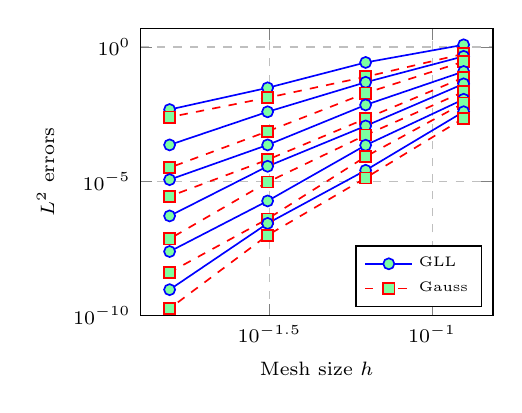
\begin{tikzpicture}
\begin{loglogaxis}[
    width=.5\textwidth,
    xlabel={Mesh size $h$},
    ylabel={$L^2$ errors}, 
%    xmin=.0125, 
    ymin=1e-10, ymax=5,
    legend pos=south east, legend cell align=left, legend style={font=\tiny},	
    xmajorgrids=true, ymajorgrids=true, grid style=dashed,
    legend entries={GLL, Gauss}    
]
\pgfplotsset{
cycle list={{blue, mark=*}, {red, dashed ,mark=square*}}
}
\addplot+[semithick, mark options={solid, fill=markercolor}]
coordinates{(0.125,1.2082)(0.0625,0.265357)(0.03125,0.0301118)(0.015625,0.00467693)};
\addplot+[semithick, mark options={solid, fill=markercolor}]
coordinates{(0.125,0.555586)(0.0625,0.0773534)(0.03125,0.0129171)(0.015625,0.0024363)};
\addplot+[semithick, mark options={solid, fill=markercolor}]
coordinates{(0.125,0.448878)(0.0625,0.0485323)(0.03125,0.00385418)(0.015625,0.000225396)};
\addplot+[semithick, mark options={solid, fill=markercolor}]
coordinates{(0.125,0.287685)(0.0625,0.0190431)(0.03125,0.000721055)(0.015625,3.19095e-05)};
\addplot+[semithick, mark options={solid, fill=markercolor}]
coordinates{(0.125,0.122081)(0.0625,0.00694351)(0.03125,0.000224524)(0.015625,1.14555e-05)};
\addplot+[semithick, mark options={solid, fill=markercolor}]
coordinates{(0.125,0.0731583)(0.0625,0.00213914)(0.03125,6.32128e-05)(0.015625,2.73037e-06)};
\addplot+[semithick, mark options={solid, fill=markercolor}]
coordinates{(0.125,0.0424351)(0.0625,0.00114569)(0.03125,3.59697e-05)(0.015625,5.09643e-07)};
\addplot+[semithick, mark options={solid, fill=markercolor}]
coordinates{(0.125,0.0215298)(0.0625,0.000523714)(0.03125,9.27521e-06)(0.015625,7.14031e-08)};
\addplot+[semithick, mark options={solid, fill=markercolor}]
coordinates{(0.125,0.0112838)(0.0625,0.000219049)(0.03125,1.84304e-06)(0.015625,2.40402e-08)};
\addplot+[semithick, mark options={solid, fill=markercolor}]
coordinates{(0.125,0.00809138)(0.0625,8.23415e-05)(0.03125,3.95565e-07)(0.015625,4.01268e-09)};
\addplot+[semithick, mark options={solid, fill=markercolor}]
coordinates{(0.125,0.00388316)(0.0625,2.55074e-05)(0.03125,2.68102e-07)(0.015625,9.13754e-10)};
\addplot+[semithick, mark options={solid, fill=markercolor}]
coordinates{(0.125,0.00222029)(0.0625,1.33111e-05)(0.03125,9.72405e-08)(0.015625,1.81386e-10)};

\end{loglogaxis}
\end{tikzpicture}
}
\only<2>{
\raisebox{3.5em}{\includegraphics[width=.475\textwidth]{figs/warp2d_a125.png}}
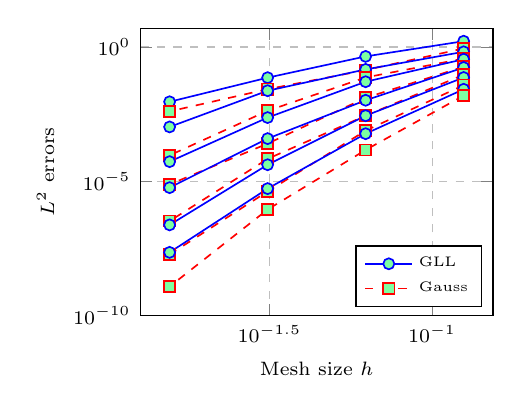
\begin{tikzpicture}
\begin{loglogaxis}[
    width=.5\textwidth,
    xlabel={Mesh size $h$},
    ylabel={$L^2$ errors}, 
%    xmin=.0125,
    ymin=1e-10, ymax=5,
    legend pos=south east, legend cell align=left, legend style={font=\tiny},	
    xmajorgrids=true, ymajorgrids=true, grid style=dashed,
    legend entries={GLL, Gauss}    
]
\pgfplotsset{
cycle list={{blue, mark=*}, {red, dashed ,mark=square*}}
}
\addplot+[semithick, mark options={solid, fill=markercolor}]
coordinates{(0.125,1.64274)(0.0625,0.445945)(0.03125,0.0720148)(0.015625,0.0091066)};
\addplot+[semithick, mark options={solid, fill=markercolor}]
coordinates{(0.125,0.882247)(0.0625,0.138116)(0.03125,0.0268145)(0.015625,0.0039945)};
\addplot+[semithick, mark options={solid, fill=markercolor}]
coordinates{(0.125,0.662165)(0.0625,0.146131)(0.03125,0.0234934)(0.015625,0.00105368)};
\addplot+[semithick, mark options={solid, fill=markercolor}]
coordinates{(0.125,0.368084)(0.0625,0.0734059)(0.03125,0.00420438)(0.015625,9.19378e-05)};
\addplot+[semithick, mark options={solid, fill=markercolor}]
coordinates{(0.125,0.349184)(0.0625,0.0508268)(0.03125,0.00234785)(0.015625,5.36192e-05)};
\addplot+[semithick, mark options={solid, fill=markercolor}]
coordinates{(0.125,0.183472)(0.0625,0.0127617)(0.03125,0.000251929)(0.015625,7.6013e-06)};
\addplot+[semithick, mark options={solid, fill=markercolor}]
coordinates{(0.125,0.171986)(0.0625,0.0103578)(0.03125,0.000386834)(0.015625,5.76284e-06)};
\addplot+[semithick, mark options={solid, fill=markercolor}]
coordinates{(0.125,0.0924215)(0.0625,0.00276519)(0.03125,6.80528e-05)(0.015625,3.27246e-07)};
\addplot+[semithick, mark options={solid, fill=markercolor}]
coordinates{(0.125,0.0729963)(0.0625,0.00276104)(0.03125,4.11305e-05)(0.015625,2.36125e-07)};
\addplot+[semithick, mark options={solid, fill=markercolor}]
coordinates{(0.125,0.0378013)(0.0625,0.0007649)(0.03125,4.15848e-06)(0.015625,1.8685e-08)};
\addplot+[semithick, mark options={solid, fill=markercolor}]
coordinates{(0.125,0.026577)(0.0625,0.000589552)(0.03125,5.3039e-06)(0.015625,2.23719e-08)};
\addplot+[semithick, mark options={solid, fill=markercolor}]
coordinates{(0.125,0.0154563)(0.0625,0.000146207)(0.03125,8.83156e-07)(0.015625,1.18829e-09)};

\end{loglogaxis}
\end{tikzpicture}
}
\only<3>{
\raisebox{3.5em}{\includegraphics[width=.475\textwidth]{figs/warp2d_a25.png}}
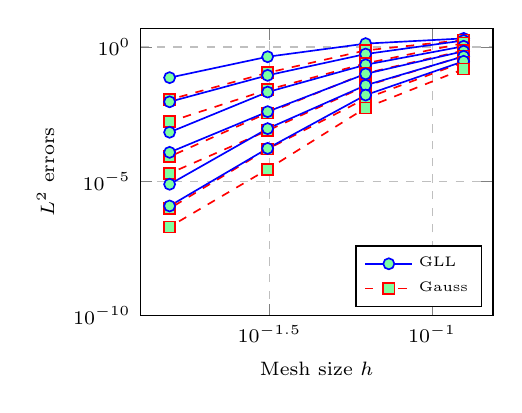
\begin{tikzpicture}
\begin{loglogaxis}[
    width=.5\textwidth,
    xlabel={Mesh size $h$},
    ylabel={$L^2$ errors}, 
%    xmin=.0125,
    ymin=1e-10, ymax=5,
    legend pos=south east, legend cell align=left, legend style={font=\tiny},	
    xmajorgrids=true, ymajorgrids=true, grid style=dashed,
    legend entries={GLL, Gauss}    
]
\pgfplotsset{
cycle list={{blue, mark=*}, {red, dashed ,mark=square*}}
}
\addplot+[semithick, mark options={solid, fill=markercolor}]
coordinates{(0.125,2.08578)(0.0625,1.33668)(0.03125,0.433653)(0.015625,0.0721002)};
\addplot+[semithick, mark options={solid, fill=markercolor}]
coordinates{(0.125,1.82833)(0.0625,0.746283)(0.03125,0.11006)(0.015625,0.0110115)};
\addplot+[semithick, mark options={solid, fill=markercolor}]
coordinates{(0.125,1.74649)(0.0625,0.546097)(0.03125,0.0879841)(0.015625,0.0090851)};
\addplot+[semithick, mark options={solid, fill=markercolor}]
coordinates{(0.125,1.39268)(0.0625,0.245852)(0.03125,0.0255562)(0.015625,0.00165226)};
\addplot+[semithick, mark options={solid, fill=markercolor}]
coordinates{(0.125,1.06289)(0.0625,0.218361)(0.03125,0.0209471)(0.015625,0.000665425)};
\addplot+[semithick, mark options={solid, fill=markercolor}]
coordinates{(0.125,0.740071)(0.0625,0.105075)(0.03125,0.003505)(0.015625,8.26421e-05)};
\addplot+[semithick, mark options={solid, fill=markercolor}]
coordinates{(0.125,0.695283)(0.0625,0.0996971)(0.03125,0.00390099)(0.015625,0.000118992)};
\addplot+[semithick, mark options={solid, fill=markercolor}]
coordinates{(0.125,0.457324)(0.0625,0.0354479)(0.03125,0.000767746)(0.015625,1.95823e-05)};
\addplot+[semithick, mark options={solid, fill=markercolor}]
coordinates{(0.125,0.449493)(0.0625,0.0374955)(0.03125,0.000909834)(0.015625,7.70064e-06)};
\addplot+[semithick, mark options={solid, fill=markercolor}]
coordinates{(0.125,0.274721)(0.0625,0.0120499)(0.03125,0.000157175)(0.015625,9.61243e-07)};
\addplot+[semithick, mark options={solid, fill=markercolor}]
coordinates{(0.125,0.294238)(0.0625,0.0162153)(0.03125,0.000166829)(.015625,1.19661e-06)};
\addplot+[semithick, mark options={solid, fill=markercolor}]
coordinates{(0.125,0.150916)(0.0625,0.00538908)(0.03125,2.79182e-05)(.015625,1.98845e-07)};
\end{loglogaxis}
\end{tikzpicture}
}
\end{overlayarea}
\caption{$L^2$ errors for the 2D isentropic vortex at time $T=5$ for degree $N = 2,\ldots,7$ GLL and Gauss collocation schemes (similar behavior in 3D).}
\end{figure}
}

\frame{
\frametitle{Shock vortex interaction}
\vspace{-.5em}
\begin{figure}
\centering
\begin{overlayarea}{\textwidth}{.45\textheight}
\only<1>{
\subfloat[Entropy conservative flux, $T = .3$]{\includegraphics[width=.49\textwidth]{figs/shockVortexTp3_EC.png}}
\hspace{.05em}
\subfloat[Entropy conservative flux, $T = .7$]{\includegraphics[width=.49\textwidth]{figs/shockVortexTp7_EC.png}}
}
\only<2>{
\subfloat[Lax-Friedrichs flux, $T = .3$]{\includegraphics[width=.49\textwidth]{figs/shockVortexTp3_LF.png}}
\hspace{.05em}
\subfloat[Lax-Friedrichs flux, $T = .7$]{\includegraphics[width=.49\textwidth]{figs/shockVortexTp7_LF.png}}\
}
\only<3>{
\subfloat[Matrix dissipation flux, $T = .3$]{\includegraphics[width=.49\textwidth]{figs/shockVortexTp3.png}}
\hspace{.05em}
\subfloat[Matrix dissipation flux, $T = .7$]{\includegraphics[width=.49\textwidth]{figs/shockVortexTp7.png}}
}
\only<4>{
\subfloat[Matrix dissipation flux, $T = .3$]{\includegraphics[width=.485\textwidth]{figs/shockVortexT3.png}}
\hspace{.05em}
\subfloat[Matrix dissipation flux, $T = .7$]{\includegraphics[width=.49\textwidth]{figs/shockVortexT7.png}}
}
\end{overlayarea}
\caption{Shock vortex interaction problem using high order entropy stable Gauss collocation schemes with $N=4, h = 1/100$.  }
\label{fig:shockvort}
\end{figure}


\let\thefootnote\relax\footnotetext{\tiny Winters, Derigs, Gassner, and Walch (2017). \textit{A uniquely defined entropy stable matrix dissipation operator for high Mach number ideal MHD and compressible Euler simulations.}}
}


\subsection{Hybrid and non-conforming meshes}
\frame[noframenumbering]{
\frametitle{Talk outline}
\tableofcontents[currentsection,currentsubsection]
}


\frame{
\frametitle{Mixed quadrilateral-triangle meshes}

\vspace{-1em}
\begin{figure}
\centering
\subfloat[No SBP (tri.\ under-integrated)]{\includegraphics[width=.425\textwidth]{figs/hybrid2D.png}}
\hspace{1em}
\subfloat[No SBP (quad.\ under-integrated)]{\includegraphics[width=.425\textwidth]{figs/hybrid2D_GQ.png}}
\end{figure}

\begin{itemize}
\item SBP property requires \note{sufficiently accurate quadrature}.
\item \note{Skew-symmetric formulation} relaxes requirements on quadrature accuracy for entropy stability:
\end{itemize}
\[
\bm{M}\td{\hat{\bm{u}}}{t} + \sum_{i=1}^d\LRs{\begin{array}{c}
\bm{V}_q \\ \bm{V}_f\end{array}}^T \LRp{\LRp{\bm{Q}^i_N-\LRp{\bm{Q}^i_N}^T} \circ \bm{F}^i_S}\bm{1} + \bm{V}_f^T\bm{B}_i \bm{f}^i_S(\tilde{\bm{u}}^+,\tilde{\bm{u}}) = 0.
\]
}

\frame{
\frametitle{Numerical results: mixed triangle-quadrilateral meshes}
\setcounter{subfigure}{0}
\begin{figure}
\centering
\subfloat[Coarse hybrid mesh]{\raisebox{2.25em}{\includegraphics[width=.45\textwidth]{figs/hybrid_mesh.png}}}
\hspace{.25em}
\subfloat[Convergence for $N = 1,2,3,4$]{
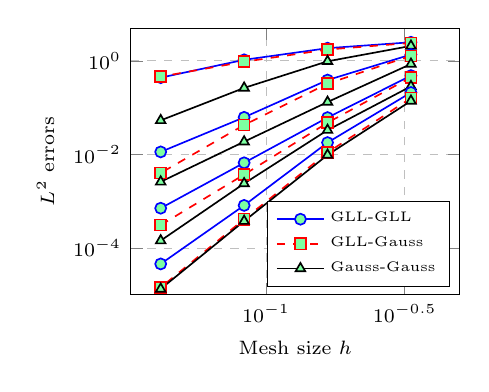
\begin{tikzpicture}
\begin{loglogaxis}[
    width=.475\textwidth,
    xlabel={Mesh size $h$},
    ylabel={$L^2$ errors}, 
    xmax=.5,
    ymin=1e-5, ymax=5,
    legend pos=south east, legend cell align=left, legend style={font=\tiny},	
    xmajorgrids=true, ymajorgrids=true, grid style=dashed,
    legend entries={GLL-GLL, GLL-Gauss, Gauss-Gauss} 
]
\pgfplotsset{
cycle list={{blue, mark=*}, {red, dashed ,mark=square*},{black ,mark=triangle*}}
}
\addplot+[semithick, mark options={solid, fill=markercolor}]
coordinates{(0.333333,2.50656)(0.166667,1.874)(0.0833333,1.05647)(0.0416667,0.438926)};
\addplot+[semithick, mark options={solid, fill=markercolor}]
coordinates{(0.333333,2.42633)(0.166667,1.75142)(0.0833333,0.958902)(0.0416667,0.462137)};
\addplot+[semithick, mark options={solid, fill=markercolor}]
coordinates{(0.333333,2.09363)(0.166667,0.981664)(0.0833333,0.264928)(0.0416667,0.0536376)};
\addplot+[semithick, mark options={solid, fill=markercolor}]
coordinates{(0.333333,1.36947)(0.166667,0.390076)(0.0833333,0.0623387)(0.0416667,0.011361)};
\addplot+[semithick, mark options={solid, fill=markercolor}]
coordinates{(0.333333,1.28187)(0.166667,0.326338)(0.0833333,0.0427717)(0.0416667,0.00402484)};
\addplot+[semithick, mark options={solid, fill=markercolor}]
coordinates{(0.333333,0.859449)(0.166667,0.132239)(0.0833333,0.0187852)(0.0416667,0.0026063)};
\addplot+[semithick, mark options={solid, fill=markercolor}]
coordinates{(0.333333,0.48545)(0.166667,0.0615538)(0.0833333,0.00665061)(0.0416667,0.000711264)};
\addplot+[semithick, mark options={solid, fill=markercolor}]
coordinates{(0.333333,0.446407)(0.166667,0.0477486)(0.0833333,0.00372164)(0.0416667,0.000309705)};
\addplot+[semithick, mark options={solid, fill=markercolor}]
coordinates{(0.333333,0.286258)(0.166667,0.0331728)(0.0833333,0.00239593)(0.0416667,0.000144346)};
\addplot+[semithick, mark options={solid, fill=markercolor}]
coordinates{(0.333333,0.211329)(0.166667,0.0179798)(0.0833333,0.000816429)(0.0416667, 4.583068530777824e-05)};
\addplot+[semithick, mark options={solid, fill=markercolor}]
coordinates{(0.333333,0.160937)(0.166667,0.0110045)(0.0833333,0.00041413)(0.0416667, 1.438708299584088e-05)};
\addplot+[semithick, mark options={solid, fill=markercolor}]
coordinates{(0.333333,0.13975)(0.166667,0.00977304)(0.0833333,0.00037731)(0.0416667, 1.337566281886131e-05)};
%\node at (axis cs:.55,2.5) {$N = 1$};
%\node at (axis cs:.55,.82) {$N = 2$};
%\node at (axis cs:.55,.25) {$N = 3$};
%\node at (axis cs:.55,.08) {$N = 4$};
\end{loglogaxis}
\end{tikzpicture}
}
\end{figure}

\begin{center}
The skew-symmetric formulation guarantees entropy stability for all combinations of GLL and Gauss volume and surface quadratures.
\end{center}

}


\frame{
\frametitle{Meshes with non-conforming interfaces}

%\begin{overlayarea}{\textwidth}{\textheight}

\only<1>{
\vspace{-.5em}
\begin{figure}
\centering
\subfloat[Conforming surface nodes]{\includegraphics[height=.375\textheight]{figs/mortar1.png}}
\hspace{.5em}
\subfloat[Non-conforming surface nodes]{\includegraphics[height=.375\textheight]{figs/mortar2.png}}
\end{figure}
}% only

\only<2-3>{
\begin{columns}

\column{0.45\textwidth}
\begin{figure}
\centering
\begin{overlayarea}{\textwidth}{.375\textheight}
\only<2>{\includegraphics[width=\textwidth]{figs/mortar.png}}
\only<3>{\includegraphics[width=\textwidth]{figs/mortar_coupling.png}}
\end{overlayarea}
\end{figure}

\column{0.475\textwidth}
%\setlength\arraycolsep{2em}
\begin{equation*}
%\bm{M}\td{\bm{u}_N}{t} + \begin{bmatrix} \bm{V}_q \\ \bm{V}_f \\ \bm{V}_m \end{bmatrix}^T
%\LRp{
\underbrace{\begin{bmatrix}
\bm{Q}_i-\bm{Q}_i^T & \bm{E}^T\bm{B}_i &\\
-\bm{B}_i\bm{E} &  & \bm{B}_i\tilde{\bm{E}}_m \\
& -\tilde{\bm{B}}_i{\bm{E}}_m & 
\end{bmatrix}}_{\text{modified skew operator } \bm{Q}^i_N- \LRp{\bm{Q}^i_N}^T}
%\circ \bm{F}_S}\bm{1} + \bm{V}_m^T\tilde{\bm{B}}_i\bm{f}_i^* = 0.  
%\label{eq:mortar}
\end{equation*}

\end{columns}
\vspace{.5em}
}% only


\begin{itemize}
\item<1-> Volume/surface nodes interact through $\bm{f}_S(\bm{u}_i,\bm{u}_j)$ and \note{interpolation}.
\vspace{.25em}
\item<2-> Weakly couple volume nodes to non-conforming surface nodes by adding conforming ``mortar'' (via additional blocks in $\bm{Q}_N$).
\vspace{.25em}
\item<2-> Can reformulate as an entropy stable correction to standard mortar.  
\end{itemize}

%\end{overlayarea}
}

\frame{
\frametitle{Numerical results: non-conforming meshes}

\begin{figure}
\centering
\subfloat[Coarse non-conforming mesh]{\raisebox{3em}{\includegraphics[width=.425\textwidth]{figs/noncon_mesh.png}}}
\hspace{.25em}
\subfloat[Sub-optimal rates if under-integrated]{
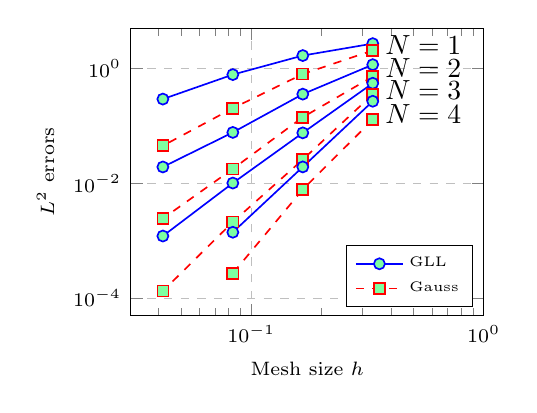
\begin{tikzpicture}
\begin{loglogaxis}[
    width=.5\textwidth,
    xlabel={Mesh size $h$},
    ylabel={$L^2$ errors}, 
    xmax=1,
    ymin=5e-5, ymax=5,
    legend pos=south east, legend cell align=left, legend style={font=\tiny},	
    xmajorgrids=true, ymajorgrids=true, grid style=dashed,
    legend entries={GLL, Gauss}    
]
\pgfplotsset{
cycle list={{blue, mark=*}, {red, dashed ,mark=square*}}
}
\addplot+[semithick, mark options={solid, fill=markercolor}]
coordinates{(0.333333,2.6993)(0.166667,1.6718)(0.0833333,0.7792)(0.0416667,0.29211)};
\addplot+[semithick, mark options={solid, fill=markercolor}]
coordinates{(0.333333,2.0534)(0.166667,0.7966)(0.0833333,0.2022)(0.0416667,0.0449413)};
\addplot+[semithick, mark options={solid, fill=markercolor}]
coordinates{(0.333333,1.1609)(0.166667,0.3562)(0.0833333,0.0768)(0.0416667,0.0192197)};
\addplot+[semithick, mark options={solid, fill=markercolor}]
coordinates{(0.333333,0.7191)(0.166667,0.141)(0.0833333,0.0178)(0.0416667,0.00243087)};
\addplot+[semithick, mark options={solid, fill=markercolor}]
coordinates{(0.333333,0.551145)(0.166667,0.0754237)(0.0833333,0.0100808)(0.0416667,0.00120633)};
\addplot+[semithick, mark options={solid, fill=markercolor}]
coordinates{(0.333333,0.352706)(0.166667,0.0258415)(0.0833333,0.00211953)(0.0416667,0.000132969)};
\addplot+[semithick, mark options={solid, fill=markercolor}]
coordinates{(0.333333,0.267668)(0.166667,0.0192603)(0.0833333,0.00140341)};
\addplot+[semithick, mark options={solid, fill=markercolor}]
coordinates{(0.333333,0.128217)(0.166667,0.00779943)(0.0833333,0.000270803)};
\node at (axis cs:.55,2.5) {$N = 1$};
\node at (axis cs:.55,1.0) {$N = 2$};
\node at (axis cs:.55,.42) {$N = 3$};
\node at (axis cs:.55,.16) {$N = 4$};
\end{loglogaxis}
\end{tikzpicture}
}
\end{figure}

\begin{center}
The skew-symmetric formulation guarantees entropy stability for both GLL and Gauss quadratures, but Gauss is more accurate.
\end{center}
}



%% =================================================

\frame{
\frametitle{Summary and future work}

\begin{itemize}
\item Entropy stable high order discontinuous Galerkin methods: semi-discrete stability, improved robustness.
\vspace{.25em}
\item Additional work required for strong shocks, positivity preservation.  
\vspace{.25em}
\item Current work: hybrid and non-conforming meshes, multi-GPU.
\vspace{.25em}
\item This work is supported by DMS-1719818 and DMS-1712639. 
\end{itemize}
\vspace{.25em}
\begin{center}
Thank you!  Questions?
\vspace{.25em}

{\includegraphics[width=.15\textwidth]{figs/nsf.jpg}}
\end{center}

%\let\thefootnote\relax\footnotetext{\tiny Extra slides on GPU efficiency available!}
\let\thefootnote\relax\footnotetext{\tiny Chan, Del Rey Fernandez, Carpenter (2018). \textit{Efficient entropy stable Gauss collocation methods}.}
\let\thefootnote\relax\footnotetext{\tiny Chan, Wilcox (2018). \textit{On discretely entropy stable weight-adjusted DG methods: curvilinear meshes}.}
\let\thefootnote\relax\footnotetext{\tiny Chan, Hewett, and Warburton (2016). \textit{Weight-adjusted discontinuous Galerkin methods: curvilinear meshes}.}
\let\thefootnote\relax\footnotetext{\tiny Chan (2017). \textit{On discretely entropy conservative and entropy stable discontinuous Galerkin methods.}}

}

%% =================================================


\begin{frame}[noframenumbering]
\frametitle{Additional slides }
\end{frame}


\frame[noframenumbering]{
\frametitle{Over-integration is ineffective without $L^2$ projection}

\begin{figure}[!h]
\centering
\begingroup
\captionsetup[subfigure]{width=.5\textwidth}
\subfloat[$(N+1)$ points]{\includegraphics[width=.45\textwidth]{figs/sbpGLL.png}}
\hspace{1em}
\subfloat[$(N+4)$ points]{\includegraphics[width=.45\textwidth]{figs/sbpGLLNp4.png}}
\endgroup
%\subfloat[$(N+4)$ point GLL]{\includegraphics[width=.32\textwidth]{figs/dsbpGLLNp4.png}}
\caption{Numerical results for the Sod shock tube for $N=4$ and $K=32$ elements.  Over-integrating by increasing the number of quadrature points does not improve solution quality.  }
\label{fig:sbpq}
\end{figure}
}

\frame[noframenumbering]{
\frametitle{On CFL restrictions}

\begin{itemize}
\item For GLL-$(N+1)$ quadrature, $\tilde{\bm{u}} = \bm{u}\LRp{P_N \bm{v}} = \bm{u}$ at GLL points.
\item For GQ-$(N+2)$, discrepancy between $L^2$ projection and interpolation.
\item Still need \note{positivity} of thermodynamic quantities for stability!
\end{itemize}
\vspace{-1em}
\begin{figure}
\centering
\subfloat[${v}_3(x), \LRp{P_N v_3}(x)$]{\includegraphics[width=.45\textwidth]{figs/sineShockQ3Compare.png}}
\hspace{1em}
\subfloat[$\rho(x), \rho\LRp{\LRp{P_N \bm{v}}(x)}$]{\includegraphics[width=.44\textwidth]{figs/sineShockDensityCompare.png}}
\end{figure}
}


%
%\frame[noframenumbering]{
%\frametitle{Asymptotically non-affine geometric mappings}
%
%%\only<1-2>{
%%Comparison with $L^2$ projection and Low-Storage Curvilinear DG
%%\[
%%\tilde{\phi}_i = \frac{\phi_i}{\sqrt{J}}, \qquad \bm{M}_{ij} = \int_{D^k} \tilde{\phi}_j\tilde{\phi}_i J = \int_{\widehat{D}} \phi_j\phi_i = \widehat{\bm{M}}_{ij}.
%%\]
%%\vspace{-2em}
%%}
%
%\begin{figure}
%\begin{overlayarea}{\textwidth}{.6\textheight}
%\centering
%\only<1>{
%\vspace{-2em}
%Similar rate of convergence for both $L^2$ projection and WADG.
%\vspace{1em}
%
%\subfloat{
%\includegraphics[width=.37\textwidth]{figs/randunif1.png}
%}
%\subfloat{
%\begin{tikzpicture}
%\begin{loglogaxis}[
%	legend cell align=left,
%	        legend style={font=\tiny},
%	width=.49\textwidth,
%    xlabel={Mesh size $h$},
%    ylabel={$L^2$ error},
%    xmin=.005, xmax=1,
%    ymin=1e-10, ymax=1e-1,
%    legend pos=south east,
%    xmajorgrids=true,
%    ymajorgrids=true,
%    grid style=dashed,
%] 
%\addplot[color=blue,mark=*,mark size=3,semithick, mark options={fill=markercolor}]
%coordinates{(0.5,0.00943375)(0.25,0.00276313)(0.125,0.000415615)(0.0625,6.56974e-05)(0.03125,8.95162e-06)(0.015625,1.14109e-06)};
%%\addplot[color=black,mark=diamond*,mark size=4,semithick, mark options={fill=markercolor}]
%%coordinates{(0.5,0.0134065)(0.25,0.012209)(0.125,0.004612)(0.0625,0.00163555)(0.03125,0.000458367)(0.015625,0.00011822)};
%\addplot[color=red,mark=square*,mark size=3,semithick, mark options={fill=markercolor}]
%coordinates{(0.5,0.00990795)(0.25,0.00389737)(0.125,0.00064227)(0.0625,0.000123078)(0.03125,1.80455e-05)(0.015625,2.28866e-06)};
%\logLogSlopeTriangleFlip{0.325}{0.125}{0.525}{3}{red};
%\logLogSlopeTriangle{0.325}{0.125}{0.375}{3}{blue};
%
%%\legend{$L^2$ projection, LSC-DG, WADG}
%\legend{$L^2$ projection, WADG}
%\end{loglogaxis}
%\end{tikzpicture}
%}
%\caption{Curvilinear element constructed through random perturbation for $N = 3$.}
%}
%\only<2>{
%\vspace{-2em}
%High order convergence \textcolor{red}{slowed} by growth of $\nor{J}_{W^{N+1,\infty}} = O(h)$.
%\vspace{1em}
%
%\subfloat{
%\includegraphics[width=.37\textwidth]{figs/arnoldmesh1.png}
%}
%\subfloat{
%\begin{tikzpicture}
%\begin{loglogaxis}[
%	legend cell align=left,
%	        legend style={font=\tiny},	
%	width=.49\textwidth,
%    xlabel={Mesh size $h$},
%    ylabel={$L^2$ error},
%    xmin=.005, xmax=1,
%    ymin=1e-10, ymax=1e-1,
%    legend pos=south east,
%    xmajorgrids=true,
%    ymajorgrids=true,
%    grid style=dashed,
%] 
%% adding this 2x because pgfplots dashes the line for some reason...
%\addplot[color=blue,mark=*,mark size=3,semithick, mark options={fill=markercolor}]
%coordinates{(0.5,0.00145465)(0.25,0.000140693)(0.125,1.17949e-05)(0.0625,8.58138e-07)(0.03125,5.78543e-08)(0.015625,3.75483e-09)};
%%\addplot[color=black,mark=diamond*,mark size=4,semithick, mark options={fill=markercolor}]
%%coordinates{(0.5,0.00159198)(0.25,0.000658818)(0.125,0.000619747)(0.0625,0.000677173)(0.03125,0.00073964)(0.015625,0.000782687)};
%\addplot[color=red,mark=square*,mark size=3,semithick, mark options={fill=markercolor}]
%coordinates{(0.5,0.00148852)(0.25,0.000176325)(0.125,2.60169e-05)(0.0625,3.94602e-06)(0.03125,5.58752e-07)(0.015625,7.47639e-08)};
%\logLogSlopeTriangleFlip{0.325}{0.125}{0.37}{3}{red};
%\logLogSlopeTriangle{0.35}{0.125}{0.12}{4}{blue};
%
%%\legend{$L^2$ projection, LSC-DG, WADG}
%\legend{$L^2$ projection, WADG}
%\end{loglogaxis}
%\end{tikzpicture}
%}
%\caption{Arnold-type element with $\nor{J}_{W^{N+1,\infty}} = O(h^{-1})$ for $N = 3$.}
%}
%\only<3>{
%\vspace{-2em}
%High order convergence \textcolor{red}{slowed} by growth of $\nor{J}_{W^{N+1,\infty}} = O(h^{-N})$.
%\vspace{1em}
%
%\subfloat{
%\includegraphics[width=.37\textwidth]{figs/curvarnold2ref.png}
%}
%\subfloat{
%\begin{tikzpicture}
%\begin{loglogaxis}[
%legend style={font=\tiny},
%	legend cell align=left,
%	width=.49\textwidth,
%    xlabel={Mesh size $h$},
%    ylabel={$L^2$ error},
%    xmin=.0025, xmax=1,
%    ymin=1e-7, ymax=1e-0,
%    legend pos=south east,
%    xmajorgrids=true,
%    ymajorgrids=true,
%    grid style=dashed,
%] 
%% adding this 2x because pgfplots dashes the line for some reason...
%\addplot[color=blue,mark=*,mark size=3,semithick, mark options={fill=markercolor}]
%coordinates{(0.5,0.0149174)(0.25,0.00576658)(0.125,0.00165616)(0.0625,0.000433839)(0.03125,0.000110389)(0.015625,2.78024e-05)};
%%\addplot[color=black,mark=diamond*,mark size=4,semithick, mark options={fill=markercolor}]
%%coordinates{(0.5,0.018737)(0.25,0.0147278)(0.125,0.0117761)(0.0625,0.0110991)(0.03125,0.0112431)(0.015625,0.0114663)};
%\addplot[color=red,mark=square*,mark size=3,semithick, mark options={fill=markercolor}]
%coordinates{(0.5,0.0165783)(0.25,0.00872368)(0.125,0.00464969)(0.0625,0.00253621)(0.03125,0.00134518)(0.015625,0.000695124)};
%\logLogSlopeTriangleFlip{0.41}{0.15}{0.6}{1}{red};
%\logLogSlopeTriangle{0.41}{0.15}{0.25}{2}{blue};
%
%%\node at (axis cs:.03,2.1e-07) {$a = 10^{-1}$};
%
%%\legend{$L^2$ proj, LSC-DG, WADG}
%\legend{$L^2$ proj, WADG}
%\end{loglogaxis}
%\end{tikzpicture}
%}
%\caption{Moderately warped curved Arnold-type element for $N = 3$.}
%}
%\only<4>{
%\vspace{-2em}
%High order convergence is \textcolor{red}{stalled} by growth of $\nor{J}_{W^{N+1,\infty}} = O(h^{-(N+1)})$.
%\vspace{1em}
%
%\subfloat{
%\includegraphics[width=.37\textwidth]{figs/curvarnold1ref.png}
%}
%\subfloat{
%\begin{tikzpicture}
%\begin{loglogaxis}[
%legend style={font=\tiny},
%	legend cell align=left,
%	width=.49\textwidth,
%    xlabel={Mesh size $h$},
%    ylabel={$L^2$ error},
%    xmin=.0025, xmax=1,
%    ymin=1e-7, ymax=1e-0,
%    legend pos=south east,
%    xmajorgrids=true,
%    ymajorgrids=true,
%    grid style=dashed,
%] 
%\addplot[color=blue,mark=*,mark size=3,semithick, mark options={fill=markercolor}]
%coordinates{(0.5,0.038232)(0.25,0.0144542)(0.125,0.00400233)(0.0625,0.000991275)(0.03125,0.000234827)(0.015625,5.4896e-05)};
%%\addplot[color=black,mark=diamond*,mark size=4,semithick, mark options={fill=markercolor}]
%%coordinates{(0.5,0.0579895)(0.25,0.052133)(0.125,0.0462352)(0.0625,0.0434683)(0.03125,0.0394193)(0.015625,0.032696)};
%\addplot[color=red,mark=square*,mark size=3,semithick, mark options={fill=markercolor}]
%coordinates{(0.5,0.0681969)(0.25,0.0751338)(0.125,0.0744307)(0.0625,0.0695447)(0.03125,0.0656228)(0.015625,0.0653247)};
%%\logLogSlopeTriangleFlip{0.3}{0.125}{0.475}{1}{red};
%\logLogSlopeTriangleFlip{0.425}{0.15}{0.45}{2}{blue};
%
%%\node at (axis cs:.03,2.1e-07) {$a = 10^{-1}$};
%
%%\legend{$L^2$ proj, LSC-DG, WADG}
%\legend{$L^2$ proj, WADG}
%\end{loglogaxis}
%\end{tikzpicture}
%}
%\caption{Heavily warped curved Arnold-type element for $N = 3$.}
%}
%
%\end{overlayarea}
%
%\end{figure}
%}
%
%\frame[noframenumbering]{
%\frametitle{Weight-adjusted DG: local conservation}
%
%\begin{itemize}
%\item \textcolor{red}{Con:} loss of local conservation for $w(x) \not\in P^N$!
%\vspace{1em}
%\item \textcolor{blue}{Pro:} superconvergence of conservation error
%\begin{align*}
%&\LRb{\int_{\widehat{D}} w p(\bm{x},t) - \int_{\widehat{D}} T_{1/w}^{-1} p(\bm{x},t)} \\
%\text{Conservation error}
%&\leq C \textcolor{red}{h^{2N+2}} \nor{w}_{W^{N+1,\infty}}\nor{p}_{W^{N+1,2}}
%\end{align*}
%where $C$ depends on mesh quality and max/min values of $w$.
%\vspace{1em}
%\item \textcolor{blue}{Pro:} can restore local conservation with rank-1 update (Shermann-Morrison).
%\end{itemize}
%}
%
%
%\frame[noframenumbering]{
%\frametitle{Effect of conservation on shock speeds}
%
%\begin{itemize}
%\item Weighted Burgers' equation, $w(x)$ curves characteristic lines.
%\[
%w(x)\pd{u}{t}{} + \frac{1}{2}\pd{u^2}{x}{} = 0.
%\]
%\item WADG yields high order convergence, correct shock speed for both $w(x)$ smooth, discontinuous (within an element).
%\end{itemize}
%%\vspace{-1em}
%\begin{overlayarea}{\textwidth}{.55\textheight}
%\only<1>{
%\begin{figure}
%\centering
%\subfloat[Smooth solution]{\includegraphics[width=.4\textwidth]{figs/burgersSmooth2.png}}
%\hspace{1em}
%\subfloat[Shock solution]{\includegraphics[width=.39\textwidth]{figs/burgersShock2.png}}
%\end{figure}
%}
%\only<2>{
%\vspace{2em}
%\begin{center}
%Best guess: {where} and {what} is locally conserved matters;\\ non-conservation of \textit{nonlinear flux} results in incorrect shock speeds.  
%\end{center}
%}
%\end{overlayarea}
%}

\frame[noframenumbering]{
\frametitle{High order DG on many-core (GPU) architectures}
\vspace{-1em}
\begin{figure}
\begin{overlayarea}{\textwidth}{.6\textheight}
\only<1>{
\centering
\includegraphics[width=.675\textwidth]{figs/gpu.pdf}
\caption{NVIDIA Maxwell GM204 GPU: 16 cores, 4 SIMD clusters of 32 units.}
}
\only<2->{
\centering
\includegraphics[width=.525\textwidth]{figs/dggpu001.png}
\caption{Thread blocks process elements, threads process degrees of freedom.}
}
%\only<3->{
%\centering
%\includegraphics[height=.25\textheight]{figs/airplane_DG.pdf}
%\includegraphics[height=.25\textheight]{figs/helicopter.png}
%\includegraphics[height=.25\textheight]{figs/airplane.png}\\
%\includegraphics[height=.25\textheight]{figs/trifoil.png}
%\includegraphics[height=.25\textheight]{figs/car.png}
%\includegraphics[height=.25\textheight]{figs/wingflow.png}
%\caption{GPU-accelerated simulations of scattering and compressible flow.}
%}
\end{overlayarea}
\end{figure}
\vspace{-.5em}
\begin{itemize}
\item<1-> Thousands of processing units organized in synchronized groups.  
\item<3-> No free lunch: \note{memory} costs (accesses, transfer, latency, storage).
\end{itemize}
\let\thefootnote\relax\footnotetext{\tiny Klockner, Warburton, Bridge, Hesthaven 2009, Nodal discontinuous Galerkin methods on graphics processors.}
}

\frame[noframenumbering]{
\frametitle{Implementing high order entropy stable DG on GPUs}

\begin{itemize}
\item ``FLOPS are free, \textbf{\emph{but}} \ldots''
\begin{center}
(bytes are expensive) / (memory is dear) /
\note{(postage is extra)}
\end{center}
\vspace{.5em}
\item Standard considerations: minimize CPU-GPU transfers, structured data layouts, reduce global memory accesses, maximize data reuse.  
\vspace{.5em}
\item Arithmetic vs memory latency: need roughly \note{$O(10)$ operations per byte} of memory accessed (high arithmetic intensity).
\vspace{.5em}
\item Standard mat-vec: \note{only $1/10 - 1/2$} FLOPS per byte!  
\end{itemize}
%\end{column}
%\end{columns}
}

\frame[noframenumbering]{
\frametitle{GPUs and flux differencing: when FLOPS are free}
\begin{figure}
\centering
\includegraphics[width=.85\textwidth]{figs/esdg_gpu.png}
\end{figure}
\vspace{-1em}
\begin{itemize}
\item High arithmetic intensity: compute while waiting for global memory.
\item On GPUs, extra operations don't increase runtime until $N \geq 9$!
\end{itemize}

\let\thefootnote\relax\footnotetext{\tiny Wintermeyer, Winters, Gassner, Warburton (2018).  \emph{An entropy stable discontinuous Galerkin method for the shallow water equations on curvilinear meshes with wet/dry fronts accelerated by GPUs}.}
}



\bibliographystyle{plain}
{\scriptsize
\bibliography{pyramids}
}

\end{document}
